\documentclass[]{book}
\usepackage{lmodern}
\usepackage{amssymb,amsmath}
\usepackage{ifxetex,ifluatex}
\usepackage{fixltx2e} % provides \textsubscript
\ifnum 0\ifxetex 1\fi\ifluatex 1\fi=0 % if pdftex
  \usepackage[T1]{fontenc}
  \usepackage[utf8]{inputenc}
\else % if luatex or xelatex
  \ifxetex
    \usepackage{mathspec}
  \else
    \usepackage{fontspec}
  \fi
  \defaultfontfeatures{Ligatures=TeX,Scale=MatchLowercase}
    \setmainfont[]{NanumGothic}
\fi
% use upquote if available, for straight quotes in verbatim environments
\IfFileExists{upquote.sty}{\usepackage{upquote}}{}
% use microtype if available
\IfFileExists{microtype.sty}{%
\usepackage{microtype}
\UseMicrotypeSet[protrusion]{basicmath} % disable protrusion for tt fonts
}{}
\usepackage[margin=1in]{geometry}
\usepackage{hyperref}
\PassOptionsToPackage{usenames,dvipsnames}{color} % color is loaded by hyperref
\hypersetup{unicode=true,
            pdftitle={Basic Statistics and Data Analysis: Korean Version},
            pdfauthor={Sanghoon Park},
            colorlinks=true,
            linkcolor=Maroon,
            citecolor=Blue,
            urlcolor=blue,
            breaklinks=true}
\urlstyle{same}  % don't use monospace font for urls
\usepackage{natbib}
\bibliographystyle{apalike}
\usepackage{color}
\usepackage{fancyvrb}
\newcommand{\VerbBar}{|}
\newcommand{\VERB}{\Verb[commandchars=\\\{\}]}
\DefineVerbatimEnvironment{Highlighting}{Verbatim}{commandchars=\\\{\}}
% Add ',fontsize=\small' for more characters per line
\usepackage{framed}
\definecolor{shadecolor}{RGB}{248,248,248}
\newenvironment{Shaded}{\begin{snugshade}}{\end{snugshade}}
\newcommand{\AlertTok}[1]{\textcolor[rgb]{0.94,0.16,0.16}{#1}}
\newcommand{\AnnotationTok}[1]{\textcolor[rgb]{0.56,0.35,0.01}{\textbf{\textit{#1}}}}
\newcommand{\AttributeTok}[1]{\textcolor[rgb]{0.77,0.63,0.00}{#1}}
\newcommand{\BaseNTok}[1]{\textcolor[rgb]{0.00,0.00,0.81}{#1}}
\newcommand{\BuiltInTok}[1]{#1}
\newcommand{\CharTok}[1]{\textcolor[rgb]{0.31,0.60,0.02}{#1}}
\newcommand{\CommentTok}[1]{\textcolor[rgb]{0.56,0.35,0.01}{\textit{#1}}}
\newcommand{\CommentVarTok}[1]{\textcolor[rgb]{0.56,0.35,0.01}{\textbf{\textit{#1}}}}
\newcommand{\ConstantTok}[1]{\textcolor[rgb]{0.00,0.00,0.00}{#1}}
\newcommand{\ControlFlowTok}[1]{\textcolor[rgb]{0.13,0.29,0.53}{\textbf{#1}}}
\newcommand{\DataTypeTok}[1]{\textcolor[rgb]{0.13,0.29,0.53}{#1}}
\newcommand{\DecValTok}[1]{\textcolor[rgb]{0.00,0.00,0.81}{#1}}
\newcommand{\DocumentationTok}[1]{\textcolor[rgb]{0.56,0.35,0.01}{\textbf{\textit{#1}}}}
\newcommand{\ErrorTok}[1]{\textcolor[rgb]{0.64,0.00,0.00}{\textbf{#1}}}
\newcommand{\ExtensionTok}[1]{#1}
\newcommand{\FloatTok}[1]{\textcolor[rgb]{0.00,0.00,0.81}{#1}}
\newcommand{\FunctionTok}[1]{\textcolor[rgb]{0.00,0.00,0.00}{#1}}
\newcommand{\ImportTok}[1]{#1}
\newcommand{\InformationTok}[1]{\textcolor[rgb]{0.56,0.35,0.01}{\textbf{\textit{#1}}}}
\newcommand{\KeywordTok}[1]{\textcolor[rgb]{0.13,0.29,0.53}{\textbf{#1}}}
\newcommand{\NormalTok}[1]{#1}
\newcommand{\OperatorTok}[1]{\textcolor[rgb]{0.81,0.36,0.00}{\textbf{#1}}}
\newcommand{\OtherTok}[1]{\textcolor[rgb]{0.56,0.35,0.01}{#1}}
\newcommand{\PreprocessorTok}[1]{\textcolor[rgb]{0.56,0.35,0.01}{\textit{#1}}}
\newcommand{\RegionMarkerTok}[1]{#1}
\newcommand{\SpecialCharTok}[1]{\textcolor[rgb]{0.00,0.00,0.00}{#1}}
\newcommand{\SpecialStringTok}[1]{\textcolor[rgb]{0.31,0.60,0.02}{#1}}
\newcommand{\StringTok}[1]{\textcolor[rgb]{0.31,0.60,0.02}{#1}}
\newcommand{\VariableTok}[1]{\textcolor[rgb]{0.00,0.00,0.00}{#1}}
\newcommand{\VerbatimStringTok}[1]{\textcolor[rgb]{0.31,0.60,0.02}{#1}}
\newcommand{\WarningTok}[1]{\textcolor[rgb]{0.56,0.35,0.01}{\textbf{\textit{#1}}}}
\usepackage{longtable,booktabs}
\usepackage{graphicx,grffile}
\makeatletter
\def\maxwidth{\ifdim\Gin@nat@width>\linewidth\linewidth\else\Gin@nat@width\fi}
\def\maxheight{\ifdim\Gin@nat@height>\textheight\textheight\else\Gin@nat@height\fi}
\makeatother
% Scale images if necessary, so that they will not overflow the page
% margins by default, and it is still possible to overwrite the defaults
% using explicit options in \includegraphics[width, height, ...]{}
\setkeys{Gin}{width=\maxwidth,height=\maxheight,keepaspectratio}
\IfFileExists{parskip.sty}{%
\usepackage{parskip}
}{% else
\setlength{\parindent}{0pt}
\setlength{\parskip}{6pt plus 2pt minus 1pt}
}
\setlength{\emergencystretch}{3em}  % prevent overfull lines
\providecommand{\tightlist}{%
  \setlength{\itemsep}{0pt}\setlength{\parskip}{0pt}}
\setcounter{secnumdepth}{5}
% Redefines (sub)paragraphs to behave more like sections
\ifx\paragraph\undefined\else
\let\oldparagraph\paragraph
\renewcommand{\paragraph}[1]{\oldparagraph{#1}\mbox{}}
\fi
\ifx\subparagraph\undefined\else
\let\oldsubparagraph\subparagraph
\renewcommand{\subparagraph}[1]{\oldsubparagraph{#1}\mbox{}}
\fi

%%% Use protect on footnotes to avoid problems with footnotes in titles
\let\rmarkdownfootnote\footnote%
\def\footnote{\protect\rmarkdownfootnote}

%%% Change title format to be more compact
\usepackage{titling}

% Create subtitle command for use in maketitle
\providecommand{\subtitle}[1]{
  \posttitle{
    \begin{center}\large#1\end{center}
    }
}

\setlength{\droptitle}{-2em}

  \title{Basic Statistics and Data Analysis: Korean Version}
    \pretitle{\vspace{\droptitle}\centering\huge}
  \posttitle{\par}
  \subtitle{기초 통계와 데이터 관리: 한글판}
  \author{Sanghoon Park}
    \preauthor{\centering\large\emph}
  \postauthor{\par}
      \predate{\centering\large\emph}
  \postdate{\par}
    \date{2019-11-01}

\usepackage{booktabs}
\usepackage{amsthm}
\makeatletter
\def\thm@space@setup{%
  \thm@preskip=8pt plus 2pt minus 4pt
  \thm@postskip=\thm@preskip
}
\makeatother
\usepackage{booktabs}
\usepackage{longtable}
\usepackage{array}
\usepackage{multirow}
\usepackage{wrapfig}
\usepackage{float}
\usepackage{colortbl}
\usepackage{pdflscape}
\usepackage{tabu}
\usepackage{threeparttable}
\usepackage{threeparttablex}
\usepackage[normalem]{ulem}
\usepackage{makecell}
\usepackage{xcolor}

\usepackage{kotex}
\usepackage{mathspec}
\usepackage{amsmath,amsthm}
\usepackage{graphicx}

\begin{document}
\maketitle

{
\hypersetup{linkcolor=black}
\setcounter{tocdepth}{1}
\tableofcontents
}
\hypertarget{prerequisites}{%
\chapter{Prerequisites}\label{prerequisites}}

원래 저 같은 경우에는 통계분석을 할 때 주력 툴(tool)로 STATA를 써왔습니다. 하지만 한국에서 STATA로 대학원생이 연구를 수행하는 데 있어서 한 가지 걸림돌이 되는 문제는 바로 'Copyrights'에 있습니다.

STATA는 유저들 사이에서 온라인/오프라인 등을 통하여 여러가지 매뉴얼들과 피드백이 이루어져 강력한 이점을 지닌 도구인 것은 사실이지만 그 가격이 만만치가 않습니다. 적어도 제가 석사까지 마쳤던 학교에서는 STATA를 설치하는 데 있어서 학교 차원의 지원 등은 없었기 때문에 높은 가격을 감수하고 구매하던가 혹은 어떻게든(?) 구해서 사용하는 방법밖에는 없었습니다.

그에 비해서 \textbf{R}은 오픈소스라 어느 정도 자유롭게 접근할 수 있습니다. 또한 STATA 못지 않게 폭넓게 유저들 간의 소통을 통해 매뉴얼이 제공되며, 피드백이 이루어지는 강력한 통계패키지입니다.\footnote{피드백이 잘 이루어진다는 것은 실제 연구분석에 적용되는 패키지의 활용에 대해 커뮤니티에서의 소통이 용이하고, 분석에 필요한 새로운 패키지들에 대한 접근성이 높다는 것을 의미합니다.}

정치학을 공부하는 입장에서 STATA에서 R로 갈아타는 데 가장 어려웠던 점은 초입의 진입장벽이었다고 할 수 있습니다. 일종의 Trade-offs 관계로까지 느껴졌던 것이 \textbf{R}의 유연함은 곧 어떠한 결과를 얻기 위해서는 하나하나의 요소를 유저가 직접 조합할 수 있어야 하고, 각 요소의 특성을 파악해야 한다는 것이었습니다. 예를 들어, STATA에서는 변수의 특성 등 통계학에서 일반적으로 고려하는 부분들에 집중하면 되었지만 \textbf{R}에서는 객체(objects)의 특성들(List인지, Character인지, Factor인지, Vector인지 등)을 살펴보아야 했습니다. 만약 객체 특성을 고려하지 않을 경우에 결과가 크게 달라질 수 있기 때문입니다. 이러한 진입장벽의 문제가 종종 \textbf{R}을 시작하자마자 포기하게끔 만드는 결과로 이어지는 경우를 종종 보았습니다.

이 Git은 데이터 분석의 기본을 소개하는 데 목적을 가지고 있습니다. Git에 올라오는 자료들을 이해하는 데 있어서 수학적인 배경지식은 거의 요구되지 않지만 간단한 응용수학들에 대해서는 다루게 됩니다. 이 Git의 자료들은 통계분석을 수행하는 데 필수적인 개념적 지식들을 익숙하게 하는 것에 있습니다. 또한 \textbf{R}을 이용하여 데이터 관리 및 가시화(visualization)에 필요한 실용적인 기법들을 익히는 것을 기대합니다. 나아가 정량연구(quantitative research)에서 요구되는 재현가능성(replicability)와 투명성(transparency)을 제고할 수 있는 일련의 작업환경들을 만드는 훈련을 같이 합니다. 이 Git의 내용은 어디까지나 기본적인 내용들을 담고 있기 때문에 정량연구방법을 마스터하는 첫 걸음으로써는 적절한 내용들을 담고 있을 것이라고 기대합니다. 정리하면, 이 Git의 자료들을 통해 기대되는 성과는 다음과 같습니다.

\begin{itemize}
\tightlist
\item
  데이터에서 변수들의 관계를 서술하고 평가하는 데 필요한 통계방법을 이용하고 사용할 수 있을 것입니다.
\item
  데이터를 보여주기 위해 유용한 그래픽을 활용할 수 있게 될 것입니다.
\item
  데이터 접근성과 연구 투명성 원칙들을 자신의 연구에 충분히 적용할 수 있게 될 것입니다.
\item
  \textbf{R}을 이용하여 데이터를 관리 및 분석할 수 있게 될 것입니다.
\item
  \emph{LaTex}를 이용하여 과학적 연구의 결과를 페이퍼와 발표자료 등으로 구성해낼 수 있을 것입니다.
\end{itemize}

이 Git의 주요 자료들은 다음과 같은 자료에 기초하여 작성되었습니다.

\begin{itemize}
\tightlist
\item
  Diez, David D., Christopher D. Barr, and Mine Çetinkaya-Rundel. 2019. \emph{OpenIntro Statistics. Fourth Edition}. 무료로 \href{https://www.openintro.org/stat/textbook.php?stat_book=os}{여기}에 공개되어 있습니다.
\item
  Lander, Jared P. 2013. \emph{R for Everyone: Advanced Analytics and Graphics}. ISBN-13: 978-0321888037
\end{itemize}

이외에도 추가로 다음과 같은 홈페이지의 코스들로부터 도움을 받으실 수 있습니다.

\begin{itemize}
\tightlist
\item
  통계분석에 필요한 수학적 지식의 기본적인 내용들을 다시 복습하시기에 좋은 자료입니다: \href{https://projects.iq.harvard.edu/prefresher}{Havard's Math Prefresher}
\item
  주제별로 \textbf{R}을 활용한 분석에 대한 다양한 자료를 제공합니다: \href{https://www.datacamp.com/courses/free-introduction-to-r}{DataCamp}
\end{itemize}

\textbf{R}은 일단 하나의 언어라고 생각할 수 있습니다. \textbf{R} 자체로도 함수들을 이용해 우리가 원하는 분석을 할 수 있겠지만, 굉장히 편리하고 유용한 플랫폼을 통해서 보다 용이하게, 편리하게 \textbf{R}을 사용할 수 있습니다. 바로 \emph{RStudio}입니다. \emph{RStudio}는 Graphical User Interface(GUI)로 \textbf{R}을 좀 더 직관적으로 사용하는 데 도움을 줍니다.

\begin{itemize}
\tightlist
\item
  \textbf{R}을 다운로드 하시려면 \href{https://cloud.r-project.org/}{여기}
\item
  \textbf{R}을 설치하고 나서 플랫폼으로 설치할 \href{https://www.rstudio.com/products/rstudio/download/\#download}{RStudio}
\end{itemize}

\hypertarget{intro}{%
\chapter{\texorpdfstring{Introduction to \textbf{R}}{Introduction to R}}\label{intro}}

\textbf{R}은 프로그래밍 언어에 가까운데 통계분석에도 꽤나 특화되어 있습니다. 요즘 \emph{Python} 등도 주목받고 있지만 사회과학적 정량연구에 적용하는 정도로 통계분석을 수행하는 유관 학과들에서는 \textbf{R}을 많이 사용하는 것 같습니다. \textbf{R}은 단순하지만 동시에 복합적인 조합을 통해서 여러가지 분석을 수행할 수 있기 때문입니다.\footnote{그에 관련된 포스팅은 \href{https://blog.revolutionanalytics.com/2012/07/a-big-list-of-the-things-r-can-do.html}{링크}를 참조하시기 바랍니다.}

다음 포스팅에서는 \emph{RStudio}를 이용한 \textbf{R}의 기본적인 요소들을 소개할 것입니다. \emph{RStudio}에 대한 간략한 소개는 \href{http://sphweb.bumc.bu.edu/otlt/MPH-Modules/QuantCore/PH717-R-Basics/PH717-R-Basics3.html}{다음}의 \emph{RStudio} 공식 링크에서 살펴볼 수 있습니다.

\hypertarget{uxae30uxbcf8-uxb3d9uxc791uxc5d0-uxad00uxd55c-uxc18cuxac1c}{%
\section{기본 동작에 관한 소개}\label{uxae30uxbcf8-uxb3d9uxc791uxc5d0-uxad00uxd55c-uxc18cuxac1c}}

일단 \textbf{R}에서 일반적으로 사용하는 코드를 제외하고 코멘트를 달고 싶을 때에는 \texttt{\#} 를 사용합니다. \texttt{\#} 기호 뒤에 쓴 글들은 \textbf{RStudio}에서 작동되지 않스니다. 코멘트를 작성하는 습관을 들여놓는 게 좋은데, 본인이 만들어놓은 코드와 데이터셋 이름을 까먹어서 고생하지 않도록 해주고 다른 사람이 코드를 읽을 때에도 꽤나 유용하기 때문입니다.

\begin{itemize}
\item
  작동코드를 작성하기 전에 쓰는 설명은 보통 \texttt{\#\#}로, 작동코드 옆에 병기하는 인라인 코드(in-line code)는 \texttt{\#}로 구분하여 코멘트를 작성해줍니다.

  \begin{itemize}
  \tightlist
  \item
    즉, \texttt{\#\#}은 한 줄이 아예 전체 코멘트일 때, \texttt{\#}은 \textbf{R} 코드 옆에 해당 코드의 내용에 대해 코멘트할 때 사용합니다.
  \end{itemize}
\item
  예를 들면, 아래와 같은 코드에서 첫 번째 줄은 단순히 어떠한 분석을 수행할지 알려주는 역할만 하고, 아래의 코드가 실제로 작동될 것입니다.

\begin{Shaded}
\begin{Highlighting}[]
\CommentTok{## 1+1을 계산해봅시다.}
\DecValTok{1} \OperatorTok{+}\StringTok{ }\DecValTok{1}  \CommentTok{# 답은 2}
\end{Highlighting}
\end{Shaded}

\begin{verbatim}
## [1] 2
\end{verbatim}
\end{itemize}

\textbf{R}을 배우면 배울수록, 여러가지 노하우가 체화되고 보다 효율적인 코딩을 시도하게 되는데, 일단 간단한 팁들은 \href{https://google.github.io/styleguide/Rguide.xml}{여기}에서 살펴볼 수 있습니다. 이러한 팁과 노하우들에 익숙해지면 코드를 읽고, 공유하고, 짜는 게 조금 더 쉬워질 것이라고 생각합니다.

\hypertarget{ruxc758-uxc5f0uxc0b0uxc790operations}{%
\section{\texorpdfstring{\textbf{R}의 연산자(operations)}{R의 연산자(operations)}}\label{ruxc758-uxc5f0uxc0b0uxc790operations}}

일단 사회과학을 연구하고자 하는 입장에서 \textbf{R}을 사용하고자 하니, \textbf{R}이 가진 단순한 수학연산자들이 어떻게 기능하는지를 살펴볼 필요가 있습니다.

\begin{itemize}
\item
  \textbf{R} 안에서 어떠한 수학연산자들이 있는지 살펴보고 싶다면 \emph{RStudio} 좌측 하단 콘솔에 \texttt{?"*"}라고 입력해보면 됩니다.
\item
  사실 코드블럭의 왼쪽 기호는 몰랐을 수도 있는데, 오른쪽의 의미를 모를 것이라고는 생각하지 않습니다. 따라서 자세한 설명은 넘어가고\ldots{} 이 중에서 마지막 기호는 조금 익숙해질 필요는 있습니다. 저도 아직 연구에서 변수 조작(manipulation)할 때 사용해본 적은 없는 기호입니다만, 평소에는 크게 쓸 일이 없기 때문에 까먹지 않도록 하는 것이 중요할 것 같습니다.
\item
  마지막 기호를 이용해서 할 수 있는 대표적인 작업이 루프에서 특정 변수가 홀수인지 짝수인지 구분하게 하는 것 등입니다. 만약 2로 나누어 나머지가 남으면 홀수, 남지 않으면 짝수라고 생각해볼 수 있습니다.

\begin{Shaded}
\begin{Highlighting}[]
\CommentTok{## 제곱해보기: a^b라고 할 때, a를 b만큼 곱해주는 것}
\DecValTok{3}\OperatorTok{^}\DecValTok{2} \CommentTok{#9}
\end{Highlighting}
\end{Shaded}

\begin{verbatim}
## [1] 9
\end{verbatim}

\begin{Shaded}
\begin{Highlighting}[]
\DecValTok{2}\OperatorTok{^}\DecValTok{3} \CommentTok{#8}
\end{Highlighting}
\end{Shaded}

\begin{verbatim}
## [1] 8
\end{verbatim}

\begin{Shaded}
\begin{Highlighting}[]
\CommentTok{## 나머지 구하기 : a%%b라고 할 때, a를 b로 나누고 몫이 아닌 나머지를 보여줍니다.}
\DecValTok{27} \OperatorTok\StringTok{ }\DecValTok{7} \CommentTok{#6}
\end{Highlighting}
\end{Shaded}

\begin{verbatim}
## [1] 6
\end{verbatim}

\begin{Shaded}
\begin{Highlighting}[]
\CommentTok{## 마지막으로 연산자를 가지고 계산할 때, 그리고 연산자 뿐 아니라 코딩 전체에 있어서}
\CommentTok{## 순서를 잘 고려하여 코딩해야 합니다. 아래 두 계산은 완전히 결과가 다릅니다.}
\DecValTok{3} \OperatorTok{+}\StringTok{ }\DecValTok{4} \OperatorTok{/}\StringTok{ }\DecValTok{7}
\end{Highlighting}
\end{Shaded}

\begin{verbatim}
## [1] 3.571429
\end{verbatim}

\begin{Shaded}
\begin{Highlighting}[]
\NormalTok{(}\DecValTok{3} \OperatorTok{+}\StringTok{ }\DecValTok{4}\NormalTok{) }\OperatorTok{/}\StringTok{ }\DecValTok{7}
\end{Highlighting}
\end{Shaded}

\begin{verbatim}
## [1] 1
\end{verbatim}
\end{itemize}

\hypertarget{ruxc758-uxae30uxbcf8uxc801uxc778-uxc790uxb8cc-uxc720uxd615}{%
\section{\texorpdfstring{\textbf{R}의 기본적인 자료 유형}{R의 기본적인 자료 유형}}\label{ruxc758-uxae30uxbcf8uxc801uxc778-uxc790uxb8cc-uxc720uxd615}}

\textbf{R}은 여러 가지 자료 유형을 제공합니다. 예를 들어 바로 위에서 계산할 때 사용하였던 숫자는 말 그대로 \textbf{R}에서 숫자형(numeric)으로 간주됩니다. 기본적으로 반드시 알아두어야 할 자료 유형은 다음과 같습니다.

\begin{itemize}
\tightlist
\item
  숫자형(numeric): 1.111 같이 소수점 값을 가지는 자료 유형입니다.
\item
  정수형(integer): 2와 같은 자연수를 말하는 데, 소수점 값을 갖지 않는 것. 숫자형이랑 비슷합니다.
\item
  논리형(logical): 부울리안 값(Boolean values), 참(TRUE)/거짓(FALSE)을 가지는 자료 유형입니다.
\item
  문자형(character): 문자열(text or string)의 값을 지니는 것으로 인용자("")를 사용하여 입력합니다.
\end{itemize}

자료 유형을 살펴보았으니, 잠깐 변수 배정(variable assignment)에 대해 얘기해보겠습니다. 뭐랄까, 걍 어떤 변수를 만드는 거라고 생각하면 됩니다. 변수는 통계학에서 가장 기본적인 개념 중 하나이니 따로 설명할 필요는 없을 것 같습니다.

\textbf{R}에서 우리는 어떤 값(values)을 객체(object)에 저장합니다. 이때 객체는 함수(functions)일 수도 있고 그래프(plots)이거나 혹은 데이터셋(datasets)일 수도 있습니다. 즉, 그냥 콘솔에다가 2를 치면 결과 창에 2가 나오기는 하겠지만 그거 자체를 바로 분석에 사용할 수는 없고, 사용한다고 하더라도 지속적이지 않습니다. 계속 그 값을 써먹으려면 우리도 그 값에 이름을 붙여줘야 합니다. 그 값의 성격에 따라서 그것이 저장된 용기(container)의 이름도 바뀐다고 생각하시면 편합니다. 어떤 식 자체를 저장했다면 함수의 형태로, 혹은 숫자만 넣어놨다면 걍 숫자 하나가 담긴 객체가 될 것입니다. \textbf{R}에서 변수를 배정하기 위해서는 \textless{}- 나 =의 기호를 사용하여야 한다. 사용해본 경험으로는 \textless{}-를 더 추천합니다.\footnote{참고로 R은 한글로 변수를 입력하는 기능을 제공하지 않습니다.}

\begin{Shaded}
\begin{Highlighting}[]
\CommentTok{## 사과라는 변수에다가 값을 집어넣어 보겠습니다}
\NormalTok{apples <-}\StringTok{ }\DecValTok{4}
\CommentTok{## 사과에 담긴 값을 출력합니다.}
\NormalTok{apples}
\end{Highlighting}
\end{Shaded}

\begin{verbatim}
## [1] 4
\end{verbatim}

이제는 객체/변수와 연산자를 같이 사용하여 계산을 해보겠습니다.

\begin{Shaded}
\begin{Highlighting}[]
\CommentTok{## 오렌지라는 변수에다가 값을 집어넣어 보겠습니다.}
\NormalTok{oranges <-}\StringTok{ }\DecValTok{6} 
\CommentTok{## 오렌지에는 6이 들어가 있고 사과에는 4가 들어가 있습니다. 두 개를 더해 보겠습니다.}
\NormalTok{apples }\OperatorTok{+}\StringTok{ }\NormalTok{oranges}
\end{Highlighting}
\end{Shaded}

\begin{verbatim}
## [1] 10
\end{verbatim}

다음으로는 숫자가 아니라 다른 형태의 자료를 담아보겠습니다. 주의할 점은 자료 형태가 서로 다른 변수들 끼리는 연산자를 통해 계산할 수 없다는 점입니다.

\begin{Shaded}
\begin{Highlighting}[]
\CommentTok{## 오렌지 객체에 문자열 자료를 다시 저장해봅니다.}
\NormalTok{oranges <-}\StringTok{ "six"} 
\CommentTok{## 오렌지와 사과를 더해 보겠습니다.}
\NormalTok{apples }\OperatorTok{+}\StringTok{ }\NormalTok{oranges }\CommentTok{# 에러메세지를 확인할 수 있습니다.}
\end{Highlighting}
\end{Shaded}

\begin{verbatim}
## Error in apples + oranges: non-numeric argument to binary operator
\end{verbatim}

\hypertarget{uxb17cuxb9acuxd615-uxc5f0uxc0b0uxc790-logical-operators}{%
\subsection{논리형 연산자 (Logical operators)}\label{uxb17cuxb9acuxd615-uxc5f0uxc0b0uxc790-logical-operators}}

앞서 수학연산자를 간단하게 살펴보았는데, 이번에는 논리형 연산자를 한 번 살펴 보겠습니다. 논리형 연산자는 부울리안 값(\texttt{TRUE} or \texttt{FALSE})을 나타냅니다. 논리형 연산자는 아래와 같고, 좀 더 구체적인 내용은 \href{https://www.statmethods.net/management/operators.html}{여기}에서 확인할 수 있습니다.

\begin{Shaded}
\begin{Highlighting}[]
\NormalTok{a }\OperatorTok{<}\StringTok{ }\NormalTok{b   }\CommentTok{# a가 b보다 작다는 것을 보여줍니다.}
\NormalTok{a }\OperatorTok{<=}\StringTok{ }\NormalTok{b  }\CommentTok{# a가 b보다 작거나 같다는 것을 보여줍니다.}
\NormalTok{a }\OperatorTok{>}\StringTok{ }\NormalTok{b   }\CommentTok{# a가 b보다 크다는 것을 보여줍니다.}
\NormalTok{a }\OperatorTok{>=}\StringTok{ }\NormalTok{b  }\CommentTok{# a가 b보다 크거나 같다는 것을 보여줍니다.}
\NormalTok{a }\OperatorTok{==}\StringTok{ }\NormalTok{b  }\CommentTok{# a와 b가 같다/동일하다는 것을 보여줍니다.}
\OperatorTok{!}\NormalTok{a      }\CommentTok{# a가 아니라는 의미입니다.}
\end{Highlighting}
\end{Shaded}

위의 연산자를 가지고 아래의 연습을 해보겠습니다.

\begin{Shaded}
\begin{Highlighting}[]
\CommentTok{## 1이 2보다 작을까?}
\DecValTok{1} \OperatorTok{<}\StringTok{ }\DecValTok{2} \CommentTok{# TRUE, 사실이라는 결과를 얻을 것입니다.}
\end{Highlighting}
\end{Shaded}

\begin{verbatim}
## [1] TRUE
\end{verbatim}

\begin{Shaded}
\begin{Highlighting}[]
\CommentTok{## 1 더하기 1이 3일까?}
\DecValTok{1} \OperatorTok{+}\StringTok{ }\DecValTok{1} \OperatorTok{==}\StringTok{ }\DecValTok{3} \CommentTok{# FALSE, 거짓이라는 결과를 얻을 것입니다.}
\end{Highlighting}
\end{Shaded}

\begin{verbatim}
## [1] FALSE
\end{verbatim}

\textbf{R}에서 \texttt{TRUE}는 1과 같고, \texttt{FALSE}는 0과 같습니다. 그렇다면 다음의 연습을 해보겠습니다.

\begin{Shaded}
\begin{Highlighting}[]
\NormalTok{apples <-}\StringTok{ }\DecValTok{4} 
\NormalTok{oranges <-}\StringTok{ }\OtherTok{TRUE} 
\NormalTok{apples }\OperatorTok{+}\StringTok{ }\NormalTok{oranges}
\end{Highlighting}
\end{Shaded}

\begin{verbatim}
## [1] 5
\end{verbatim}

\textbf{R}은 매우 까다롭습니다. 하나라도 다르면 기대한대로 결과가 나오지 않거나 작동하지 않고 에러메세지를 띄우기도 다반사입니다. 아래의 경우를 살펴보겠습니다.

\begin{Shaded}
\begin{Highlighting}[]
\CommentTok{## 대문자와 소문자를 가리는 R}
\NormalTok{oranges <-}\StringTok{ "six"} 
\NormalTok{Oranges <-}\StringTok{ "Six"} 
\NormalTok{oranges }\OperatorTok{==}\StringTok{ }\NormalTok{Oranges }\CommentTok{# six와 Six는 앞의 문자가 하나 다르기 때문에 }
\end{Highlighting}
\end{Shaded}

\begin{verbatim}
## [1] FALSE
\end{verbatim}

\begin{Shaded}
\begin{Highlighting}[]
                   \CommentTok{# FALSE라는 결과를 얻을 것입니다.}
\end{Highlighting}
\end{Shaded}

\hypertarget{uxbca1uxd130-vectors}{%
\section{벡터 (Vectors)}\label{uxbca1uxd130-vectors}}

앞서 변수에 대해서 얘기했는데, 이번에는 벡터에 대해서 살펴볼 것입니다. 벡터는 원하는 만큼 많은 데이터를 일차원(one-dimension)에 배열할 수 있는 형태의 자료로, \textbf{R}에서 벡터를 만들기 위해서는 \texttt{c()} 형태의 함수를 이용합니다. 이 함수의 괄호 내부에 원하는 요소들을 콤마(\texttt{,})를 이용해 배열하면 하나의 벡터에 담을 수 있습니다.

\begin{Shaded}
\begin{Highlighting}[]
\CommentTok{## 숫자형 자료들이 담긴 벡터를 만들어 보겠습니다.}
\NormalTok{num_vec <-}\StringTok{ }\KeywordTok{c}\NormalTok{(}\DecValTok{1}\NormalTok{, }\DecValTok{2}\NormalTok{, }\DecValTok{3}\NormalTok{)}
\end{Highlighting}
\end{Shaded}

이번에는 문자형 자료가 담긴 벡터와 논리형(부울리안) 값을 가진 벡터를 만들어 보겠습니다. 만들고 난 이후에 \texttt{class()}나 \texttt{typeof()} 함수를 이용하여 벡터에 어떠한 형태의 자료가 담겼는지를 확인할 수 있습니다.

\begin{Shaded}
\begin{Highlighting}[]
\CommentTok{## 여러 자료 유형을 이용하여 벡터를 만들어 보겠습니다.}
\NormalTok{mix_vec <-}\StringTok{ }\KeywordTok{c}\NormalTok{(}\DecValTok{1}\NormalTok{, }\StringTok{"Hi"}\NormalTok{, }\OtherTok{TRUE}\NormalTok{)}
\KeywordTok{class}\NormalTok{(mix_vec)  }\CommentTok{# Character라는 답을 얻게 됩니다.}
\end{Highlighting}
\end{Shaded}

\begin{verbatim}
## [1] "character"
\end{verbatim}

\begin{Shaded}
\begin{Highlighting}[]
\KeywordTok{typeof}\NormalTok{(mix_vec)}
\end{Highlighting}
\end{Shaded}

\begin{verbatim}
## [1] "character"
\end{verbatim}

하나라도 다른 유형의 자료가 벡터 안에 포함되면 기대한 결과를 얻지 못할 수 있기 때문에 항상 \texttt{class()} 함수로 확인해주는 것이 필요합니다. 그리고 벡터도 수학연산자들을 이용해 일종의 계산이 가능한데, 단, \textbf{R}은 굉장히 '까다롭다'는 것을 기억하셔야 합니다. 벡터의 경우에는 요소 하나하나를 구별해서 인식하기 때문입니다. 다음의 예를 살펴 보겠습니다.

\begin{Shaded}
\begin{Highlighting}[]
\KeywordTok{c}\NormalTok{(}\DecValTok{1}\NormalTok{, }\DecValTok{2}\NormalTok{, }\DecValTok{3}\NormalTok{) }\OperatorTok{+}\StringTok{ }\KeywordTok{c}\NormalTok{(}\DecValTok{4}\NormalTok{, }\DecValTok{5}\NormalTok{, }\DecValTok{6}\NormalTok{) }
\end{Highlighting}
\end{Shaded}

\begin{verbatim}
## [1] 5 7 9
\end{verbatim}

\begin{Shaded}
\begin{Highlighting}[]
\KeywordTok{c}\NormalTok{(}\DecValTok{1} \OperatorTok{+}\StringTok{ }\DecValTok{4}\NormalTok{, }\DecValTok{2} \OperatorTok{+}\StringTok{ }\DecValTok{5}\NormalTok{, }\DecValTok{3} \OperatorTok{+}\StringTok{ }\DecValTok{6}\NormalTok{)}
\end{Highlighting}
\end{Shaded}

\begin{verbatim}
## [1] 5 7 9
\end{verbatim}

위의 두 결과는 동일합니다. 정확히는 위의 식을 아래와 같은 식으로 \textbf{R}이 계산하여 결과를 보여준다고 하는 것이 맞을 것입니다. 다른 연산자들은 어떨까요? 그리고 만약 벡터의 요소 개수가 서로 다르면(보통 길이가 다르다고 한다) 어떻게 될까요? 다음 코드를 통해 한 번 살펴 보겠습니다.

\begin{Shaded}
\begin{Highlighting}[]
\KeywordTok{c}\NormalTok{(}\DecValTok{1}\NormalTok{, }\DecValTok{2}\NormalTok{, }\DecValTok{3}\NormalTok{) }\OperatorTok{*}\StringTok{ }\KeywordTok{c}\NormalTok{(}\DecValTok{4}\NormalTok{, }\DecValTok{5}\NormalTok{, }\DecValTok{6}\NormalTok{)     }\CommentTok{# 4, 10, 18의 결과값을 얻게 될 것입니다}
\end{Highlighting}
\end{Shaded}

\begin{verbatim}
## [1]  4 10 18
\end{verbatim}

\begin{Shaded}
\begin{Highlighting}[]
\KeywordTok{c}\NormalTok{(}\DecValTok{1}\NormalTok{, }\DecValTok{2}\NormalTok{) }\OperatorTok{+}\StringTok{ }\KeywordTok{c}\NormalTok{(}\DecValTok{4}\NormalTok{, }\DecValTok{5}\NormalTok{, }\DecValTok{6}\NormalTok{, }\DecValTok{7}\NormalTok{, }\DecValTok{8}\NormalTok{)  }\CommentTok{# 5, 7, 7, 9, 9의 결과를 얻게 되고, 두 벡터의 길이가}
\end{Highlighting}
\end{Shaded}

\begin{verbatim}
## Warning in c(1, 2) + c(4, 5, 6, 7, 8): longer object length is not a
## multiple of shorter object length
\end{verbatim}

\begin{verbatim}
## [1] 5 7 7 9 9
\end{verbatim}

\begin{Shaded}
\begin{Highlighting}[]
                            \CommentTok{# 다르다는 경고 메시지를 보게 될 것입니다.}
\KeywordTok{c}\NormalTok{(}\DecValTok{1}\NormalTok{, }\DecValTok{2}\NormalTok{) }\OperatorTok{*}\StringTok{ }\KeywordTok{c}\NormalTok{(}\DecValTok{4}\NormalTok{, }\DecValTok{5}\NormalTok{, }\DecValTok{6}\NormalTok{, }\DecValTok{7}\NormalTok{, }\DecValTok{8}\NormalTok{)  }\CommentTok{# 4, 10, 6, 14, 8}
\end{Highlighting}
\end{Shaded}

\begin{verbatim}
## Warning in c(1, 2) * c(4, 5, 6, 7, 8): longer object length is not a
## multiple of shorter object length
\end{verbatim}

\begin{verbatim}
## [1]  4 10  6 14  8
\end{verbatim}

아래의 두 코드를 살펴보면 짧은 길이의 벡터가 긴 길이의 벡터에 반복해서 계산되는 것을 알 수 있습니다. 벡터는 여러 개의 요소 값(element value)을 가질 수 있는데, 그 중에서 하나의 값을 원할 경우에는 대괄호를 이용합니다.

\begin{Shaded}
\begin{Highlighting}[]
\NormalTok{num_vec <-}\StringTok{ }\KeywordTok{c}\NormalTok{(}\DecValTok{11}\NormalTok{, }\DecValTok{21}\NormalTok{, }\DecValTok{63}\NormalTok{, }\DecValTok{44}\NormalTok{, }\DecValTok{95}\NormalTok{, }\DecValTok{86}\NormalTok{)}
\NormalTok{num_vec[}\DecValTok{3}\NormalTok{]        }\CommentTok{# 63이라는 값, 벡터의 세 번째 값을 얻게 됩니다.}
\end{Highlighting}
\end{Shaded}

\begin{verbatim}
## [1] 63
\end{verbatim}

\begin{Shaded}
\begin{Highlighting}[]
\NormalTok{num_vec[}\KeywordTok{c}\NormalTok{(}\DecValTok{1}\NormalTok{,}\DecValTok{4}\NormalTok{)]   }\CommentTok{# c(1, 4)는 첫 번째와 네 번째의 값을 산출하라는 뜻으로 11, 44라는}
\end{Highlighting}
\end{Shaded}

\begin{verbatim}
## [1] 11 44
\end{verbatim}

\begin{Shaded}
\begin{Highlighting}[]
                  \CommentTok{# 결과를 얻게될 것입니다.}
\end{Highlighting}
\end{Shaded}

\hypertarget{uxb9e4uxd2b8uxb9aduxc2a4-matrices}{%
\section{매트릭스 (Matrices)}\label{uxb9e4uxd2b8uxb9aduxc2a4-matrices}}

이번에는 매트릭스를 살펴보겠습니다. 매트릭스는 일정한 수의 열과 행으로 이루어진 두 차원(two dimension)의 집합이라고 할 수 있습니다. 이때, 매트릭스를 이루는 요소들은 같은 유형의 자료들이어야 합니다. 매트릭스는 다음과 같은 함수를 통해 만들어볼 수 있습니다.

\begin{Shaded}
\begin{Highlighting}[]
\KeywordTok{matrix}\NormalTok{(}\DecValTok{1}\OperatorTok{:}\DecValTok{12}\NormalTok{, }\DataTypeTok{byrow=}\OtherTok{TRUE}\NormalTok{, }\DataTypeTok{nrow=}\DecValTok{3}\NormalTok{)}
\end{Highlighting}
\end{Shaded}

\begin{verbatim}
##      [,1] [,2] [,3] [,4]
## [1,]    1    2    3    4
## [2,]    5    6    7    8
## [3,]    9   10   11   12
\end{verbatim}

매트릭스 함수를 이용하지 않고서라도 벡터들을 \texttt{cbind()}, 즉 열(column) 결합 또는 \texttt{rbind()}, 행(row) 결합 함수를 이용하여 합쳐 매트릭스를 만들 수 있습니다.

\begin{Shaded}
\begin{Highlighting}[]
\NormalTok{c1 <-}\StringTok{ }\DecValTok{1}\OperatorTok{:}\DecValTok{3}  \CommentTok{# 1, 2, 3}
\NormalTok{c2 <-}\StringTok{ }\DecValTok{4}\OperatorTok{:}\DecValTok{6}  \CommentTok{# 4, 5, 6}
\NormalTok{c3 <-}\StringTok{ }\DecValTok{7}\OperatorTok{:}\DecValTok{9}  \CommentTok{# 7, 8, 9}
\KeywordTok{cbind}\NormalTok{(c1,c2,c3)}
\end{Highlighting}
\end{Shaded}

\begin{verbatim}
##      c1 c2 c3
## [1,]  1  4  7
## [2,]  2  5  8
## [3,]  3  6  9
\end{verbatim}

\begin{Shaded}
\begin{Highlighting}[]
\KeywordTok{rbind}\NormalTok{(c1,c2,c3)}
\end{Highlighting}
\end{Shaded}

\begin{verbatim}
##    [,1] [,2] [,3]
## c1    1    2    3
## c2    4    5    6
## c3    7    8    9
\end{verbatim}

매트릭스를 구성하는 요소 중 하나만 선택하기 위해서 우리는 대괄호(square brackets)를 사용합니다. 대괄호라고 하지만 이 과정은 \textbf{R} 프로그래밍에서 인덱싱(indexing)이라고 하는 것입니다. 즉, 행과 열의 목록에서 필요한 요소만을 지정해서 꺼낼 수 있도록 하는 기능입니다. 매트릭스는 두 차원으로 이루어져 있기 때문에, 특정 요소 하나만을 뽑아내기 위해서는 각각 차원에 배정된 숫자, 열 번호와 행 번호가 모두 필요합니다.

\begin{Shaded}
\begin{Highlighting}[]
\NormalTok{matrix <-}\StringTok{ }\KeywordTok{matrix}\NormalTok{(}\DecValTok{1}\OperatorTok{:}\DecValTok{12}\NormalTok{, }\DataTypeTok{byrow=}\OtherTok{TRUE}\NormalTok{, }\DataTypeTok{nrow=}\DecValTok{3}\NormalTok{) }\CommentTok{# matrix라는 객체에 결과를 저장합니다.}
\NormalTok{matrix[}\DecValTok{1}\NormalTok{, }\DecValTok{2}\NormalTok{]}
\end{Highlighting}
\end{Shaded}

\begin{verbatim}
## [1] 2
\end{verbatim}

\begin{Shaded}
\begin{Highlighting}[]
\NormalTok{matrix[}\DecValTok{1}\OperatorTok{:}\DecValTok{2}\NormalTok{, }\DecValTok{2}\OperatorTok{:}\DecValTok{3}\NormalTok{]  }\CommentTok{# 더 작은 형태의 매트릭스로 추출되는 것을 확인할 수 있습니다.}
\end{Highlighting}
\end{Shaded}

\begin{verbatim}
##      [,1] [,2]
## [1,]    2    3
## [2,]    6    7
\end{verbatim}

기본적인 수학연산자를 이용하여 매트릭스도 요소들 간 계산을 할 수 있습니다.

\begin{Shaded}
\begin{Highlighting}[]
\DecValTok{11} \OperatorTok{+}\StringTok{ }\NormalTok{matrix }\CommentTok{#아까 저장해 둔 matrix 객체에 11을 더하면 모든 요소에 11이 더해집니다.}
\end{Highlighting}
\end{Shaded}

\begin{verbatim}
##      [,1] [,2] [,3] [,4]
## [1,]   12   13   14   15
## [2,]   16   17   18   19
## [3,]   20   21   22   23
\end{verbatim}

매트릭스를 이용한 계산을 자세하게 알고 싶다면 다음의 \href{https://www.statmethods.net/advstats/matrix.html}{링크}를 참조하면 좋을 듯합니다.

\hypertarget{uxb370uxc774uxd130uxd504uxb808uxc784-data-frame}{%
\section{데이터프레임 (Data frame)}\label{uxb370uxc774uxd130uxd504uxb808uxc784-data-frame}}

아마 사회과학 연구를 하게 되면 가장 많이 다루게 되는 자료 유형 중 하나일 것입니다. 일반적으로 우리가 사용하는 데이터셋은 거의 데이터 프레임 형태로 불러오게 됩니다. 데이터셋하면 일반적으로 행과 열이 있는 엑셀이 생각나 매트릭스랑 뭐가 다르지? 할 수 있는데, 아까도 말했다시피 매트릭스의 모든 요소는 동일한 유형의 자료여야 합니다. 정치학에서 많이 쓰는 자료 중 COW 데이터를 예로 들어보자면 COW 국가 코드(ccode)는 숫자형인 반면에, 국가 이름(cname)은 문자형입니다. 하나의 데이터셋에 서로 다른 유형의 자료가 담기게 되는 것입니다.

\begin{itemize}
\tightlist
\item
  국가명: 문자형
\item
  국가의 GDP: 숫자형
\item
  어떤 국가가 민주주의인지 여부: 논리형
\end{itemize}

데이터 프레임은 다양한 유형의 자료를 열과 행의 틀 안에서 저장할 수 있도록 돕습니다.

\begin{Shaded}
\begin{Highlighting}[]
\CommentTok{# R에 내장되어 있는 데이터 프레임을 불러들여 보겠습니다}
\NormalTok{mtcars}
\end{Highlighting}
\end{Shaded}

\begin{verbatim}
##                      mpg cyl  disp  hp drat    wt  qsec vs am gear carb
## Mazda RX4           21.0   6 160.0 110 3.90 2.620 16.46  0  1    4    4
## Mazda RX4 Wag       21.0   6 160.0 110 3.90 2.875 17.02  0  1    4    4
## Datsun 710          22.8   4 108.0  93 3.85 2.320 18.61  1  1    4    1
## Hornet 4 Drive      21.4   6 258.0 110 3.08 3.215 19.44  1  0    3    1
## Hornet Sportabout   18.7   8 360.0 175 3.15 3.440 17.02  0  0    3    2
## Valiant             18.1   6 225.0 105 2.76 3.460 20.22  1  0    3    1
## Duster 360          14.3   8 360.0 245 3.21 3.570 15.84  0  0    3    4
## Merc 240D           24.4   4 146.7  62 3.69 3.190 20.00  1  0    4    2
## Merc 230            22.8   4 140.8  95 3.92 3.150 22.90  1  0    4    2
## Merc 280            19.2   6 167.6 123 3.92 3.440 18.30  1  0    4    4
## Merc 280C           17.8   6 167.6 123 3.92 3.440 18.90  1  0    4    4
## Merc 450SE          16.4   8 275.8 180 3.07 4.070 17.40  0  0    3    3
## Merc 450SL          17.3   8 275.8 180 3.07 3.730 17.60  0  0    3    3
## Merc 450SLC         15.2   8 275.8 180 3.07 3.780 18.00  0  0    3    3
## Cadillac Fleetwood  10.4   8 472.0 205 2.93 5.250 17.98  0  0    3    4
## Lincoln Continental 10.4   8 460.0 215 3.00 5.424 17.82  0  0    3    4
## Chrysler Imperial   14.7   8 440.0 230 3.23 5.345 17.42  0  0    3    4
## Fiat 128            32.4   4  78.7  66 4.08 2.200 19.47  1  1    4    1
## Honda Civic         30.4   4  75.7  52 4.93 1.615 18.52  1  1    4    2
## Toyota Corolla      33.9   4  71.1  65 4.22 1.835 19.90  1  1    4    1
## Toyota Corona       21.5   4 120.1  97 3.70 2.465 20.01  1  0    3    1
## Dodge Challenger    15.5   8 318.0 150 2.76 3.520 16.87  0  0    3    2
## AMC Javelin         15.2   8 304.0 150 3.15 3.435 17.30  0  0    3    2
## Camaro Z28          13.3   8 350.0 245 3.73 3.840 15.41  0  0    3    4
## Pontiac Firebird    19.2   8 400.0 175 3.08 3.845 17.05  0  0    3    2
## Fiat X1-9           27.3   4  79.0  66 4.08 1.935 18.90  1  1    4    1
## Porsche 914-2       26.0   4 120.3  91 4.43 2.140 16.70  0  1    5    2
## Lotus Europa        30.4   4  95.1 113 3.77 1.513 16.90  1  1    5    2
## Ford Pantera L      15.8   8 351.0 264 4.22 3.170 14.50  0  1    5    4
## Ferrari Dino        19.7   6 145.0 175 3.62 2.770 15.50  0  1    5    6
## Maserati Bora       15.0   8 301.0 335 3.54 3.570 14.60  0  1    5    8
## Volvo 142E          21.4   4 121.0 109 4.11 2.780 18.60  1  1    4    2
\end{verbatim}

데이터 프레임을 분석하는 데에는 여러 가지 이용가능한 함수들이 있습니다. 대표적인 것은 데이터셋의 상위 행 일부로 자료를 간략하게 보여주는 \texttt{head()}, 반대로 아래의 행들을 보여주는 \texttt{tail()}, 데이터셋이 몇개의 관측치(obs.)와 변수들로 이루어져 있는지 그 구조(structure)를 보여주는 \texttt{str()}, 요약통계치들을 제시하는 \texttt{summary()} 등이 대표적입니다.

만약 어떤 함수였는지, 어떤 자료 유형이었는지 헷갈린다면 \textbf{R} 콘솔 창에다가 물음표 뒤에 함수 이름을 쳐보면 자세한 정보를 확인할 수 있습니다.

그러나 데이터 프레임보다 자료를 불러올 때, \texttt{tidyverse} 패키지에 속한 티블 유형으로 불러올 것을 추천합니다.

\hypertarget{uxd2f0uxbe14-tibbles}{%
\section{티블 (Tibbles)}\label{uxd2f0uxbe14-tibbles}}

티블은 \texttt{tidyverse} 패키지의 속한 함수로 티블로 저장한 자료의 유형은 데이터프레임과는 약간 차이가 있습니다. 우선 티블의 장점은 더 유저 친화적이라는 것입니다. 예를 들어, 티블은 \textbf{R} 콘솔창에서 한 눈에 확인할 수 있을 정도로 데이터의 구조를 출력해주고, 각 열의 변수들이 가지는 자료 유형이 어떤 것인지를 보여줍니다. 종종 데이터프레임으로 구성된 자료 유형을 티블로 강제 변환해야 할 경우가 있는데, 이때는 \texttt{as\_tibble()} 함수를 사용하면 된다.

일단 \texttt{tidyverse} 패키지는 \textbf{R}에 내장된 것이 아니라 Hadley Wickham이 개발한 것이기 때문에 별도로 불러와야 합니다. 패키지를 설치할 때는 \texttt{install.packages()}, 설치된 패키지를 불러올 때는 \texttt{library()} 혹은 \texttt{require()} 함수를 사용합니다.

\begin{Shaded}
\begin{Highlighting}[]
\CommentTok{## install.packages("tidyverse") # 저는 이미 설치되어 있는 상태라 코멘트 처리합니다.}
\KeywordTok{library}\NormalTok{(tidyverse)}
\end{Highlighting}
\end{Shaded}

\begin{verbatim}
## -- Attaching packages ------------- tidyverse 1.2.1 --
\end{verbatim}

\begin{verbatim}
## v ggplot2 3.2.1     v purrr   0.3.2
## v tibble  2.1.3     v dplyr   0.8.3
## v tidyr   1.0.0     v stringr 1.4.0
## v readr   1.3.1     v forcats 0.4.0
\end{verbatim}

\begin{verbatim}
## -- Conflicts ---------------- tidyverse_conflicts() --
## x dplyr::filter() masks stats::filter()
## x dplyr::lag()    masks stats::lag()
\end{verbatim}

\begin{Shaded}
\begin{Highlighting}[]
\NormalTok{mtcars <-}\StringTok{ }\KeywordTok{as_tibble}\NormalTok{(mtcars)}
\NormalTok{mtcars}
\end{Highlighting}
\end{Shaded}

\begin{verbatim}
## # A tibble: 32 x 11
##      mpg   cyl  disp    hp  drat    wt  qsec    vs    am  gear  carb
##    <dbl> <dbl> <dbl> <dbl> <dbl> <dbl> <dbl> <dbl> <dbl> <dbl> <dbl>
##  1  21       6  160    110  3.9   2.62  16.5     0     1     4     4
##  2  21       6  160    110  3.9   2.88  17.0     0     1     4     4
##  3  22.8     4  108     93  3.85  2.32  18.6     1     1     4     1
##  4  21.4     6  258    110  3.08  3.22  19.4     1     0     3     1
##  5  18.7     8  360    175  3.15  3.44  17.0     0     0     3     2
##  6  18.1     6  225    105  2.76  3.46  20.2     1     0     3     1
##  7  14.3     8  360    245  3.21  3.57  15.8     0     0     3     4
##  8  24.4     4  147.    62  3.69  3.19  20       1     0     4     2
##  9  22.8     4  141.    95  3.92  3.15  22.9     1     0     4     2
## 10  19.2     6  168.   123  3.92  3.44  18.3     1     0     4     4
## # ... with 22 more rows
\end{verbatim}

\hypertarget{uxd328uxd0a4uxc9c0-packages}{%
\section{패키지 (Packages)}\label{uxd328uxd0a4uxc9c0-packages}}

위의 \texttt{tidyverse} 패키지에 대한 설명이 사실 여기 들어와야 하는데, 티블을 설명하느라 조금 당겨서 적었습니다. 이 섹션에서 패키지에 대한 내용을 조금 더 자세하게 들여다 보도록 하겠습니다.

\textbf{R}의 패키지는 함수와 객체의 모음(collection of functions and objects)이라고 할 수 있습니다. \emph{RStudio}나 \textbf{R}을 열때마다, 여러 개의 패키지들이 자동으로 로드(load)됩니다. 어떤 패키지들이 로드되어 있는지 확인하고 싶으면 \texttt{sessionInfo()} 라는 함수를 사용하면 됩니다.

좀 더 복잡한 문제를 해결하기 위해서는 \textbf{R}에 기본적으로 탑재된 함수/패키지 이외에 추가적인 패키지를 필요로 할 때가 있습니다. 이 경우에는 다음과 같은 함수를 사용합니다.: \texttt{install.package()}

그리고 \textbf{R}에서는 패키지의 설치와 사용은 별개의 작업으로 설치된 패키지를 사용하기 위해서는 그 패키지를 로딩해야 하는데 이때는 \texttt{library()} 함수를 사용하시면 됩니다. 한 번 패키지를 설치하면 다시 설치할 필요는 없지만 새로운 \textbf{R} 세션을 시작할 때마다 매번 \texttt{library()} 함수를 이용해서 로딩을 해주어야 합니다.

\begin{Shaded}
\begin{Highlighting}[]
\CommentTok{## R 패키지 설치 예시}
\CommentTok{## foreign 함수는 version 12 이하의 STATA 파일(.dta)을 로딩할 수 있게 도와줍니다.}
\CommentTok{## install.packages("foreign")}
\CommentTok{## plyr 함수는 좀 더 복잡하고 고급스러운 자료 조작(manipulation)을 가능하게 합니다.}
\CommentTok{## install.packages("plyr")}
\CommentTok{## ggplot2 함수는 함수 가시화(visualization)를 돕습니다.}
\CommentTok{## install.packages("ggplot2")}

\CommentTok{# 설치한 패키지들을 사용하기 위하여 라이브러리(libraries)를 로드한다.}
\KeywordTok{library}\NormalTok{(foreign)}
\KeywordTok{library}\NormalTok{(plyr)}
\KeywordTok{library}\NormalTok{(ggplot2)}
\end{Highlighting}
\end{Shaded}

이렇게 로드된 패키지들의 상태와 작업창을 한 번에 저장하고 다음에 불러오고 싶을 때, 다음과 같은 패키지를 사용해 패키지들을 관리할 수도 있습니다.

\begin{Shaded}
\begin{Highlighting}[]
\CommentTok{## install.packages("session")}
\KeywordTok{library}\NormalTok{(session)}
\KeywordTok{save.session}\NormalTok{(}\DataTypeTok{file=}\StringTok{"test.Rda"}\NormalTok{) }\CommentTok{# 현재까지 불러온 패키지와 객체들이 R 스크립트가 저장된}
                              \CommentTok{# 디렉토리에 test.Rda라는 이름으로 저장됩니다.}
\CommentTok{## 나중에 Rstudio 종료 후 다시 켰을 때,}
\KeywordTok{restore.session}\NormalTok{(}\DataTypeTok{file=}\StringTok{"test.Rda"}\NormalTok{) }\CommentTok{# 기존에 저장되었던 test.Rda를 불러옵니다.}
\CommentTok{## 이때, 주의해야할 점은 R 스크립트가 저장된 디렉토리가 세션 정보를 담은 Rda가 저장된}
\CommentTok{## 디렉토리와 같아야 한다는 점입니다. 만약 다르다면 file="다른 디렉토리/file.Rda"로 }
\CommentTok{## 별도로 지정해주어야 합니다.}
\end{Highlighting}
\end{Shaded}

패키지들에 대한 더 자세한 내용을 알고 싶다면 다음의 \href{https://www.datacamp.com/community/tutorials/r-packages-guide}{링크}를 참고하면 좋습니다.

그리고 \textbf{R}이 여러 패키지를 설치하는 데 제약이 없다고는 하지만 로드는 개별 패키지별로 해야합니다. 마지막으로 한 번에 여러 개의 패키지들을 설치 및 로드할 수 있게 도와주는 패키지(패키지의 패키지\ldots{})가 있는데, 그건 \href{https://gist.github.com/stevenworthington/3178163}{여기}에서 살펴볼 수 있습니다.\footnote{Github는 알아두면 굉장히 유용한데, 이 내용은 나중에 차차 업로드하도록 하겠습니다.}

\hypertarget{uxb514uxb809uxd1a0uxb9ac-uxc0dduxc131-uxcf54uxb4dc}{%
\section{디렉토리 생성 코드}\label{uxb514uxb809uxd1a0uxb9ac-uxc0dduxc131-uxcf54uxb4dc}}

\textbf{R} 스크립트의 작성을 시작하기에 앞서, 디렉토리 생성 코드를 살펴보는 이유는 코딩하는 데 있어서 깔끔한 파일 구조를 설정하는 법을 숙지해야 효율적인 작업이 가능하기 때문입니다. 논문을 쓰는 입장이기 때문에 제 경우는 다음과 같이 폴더 구조를 정리합니다.

\begin{itemize}
\tightlist
\item
  \texttt{Main\ project} directory \(\leftarrow\) 예를 들어, {[}\texttt{2018\_FALL\_Regime\_Growth}{]}

  \begin{itemize}
  \tightlist
  \item
    폴더명 \texttt{code} subdirectory \(\leftarrow\) \textbf{R} 스크립트를 여기다 저장합니다.
  \item
    폴더명 \texttt{tables} subdirectory \(\leftarrow\) \textbf{R}에서 만든 표를 저장합니다.
  \item
    폴더명 \texttt{figures} subdirectory \(\leftarrow\) \textbf{R}에서 만든 그래프 등을 저장합니다.
  \item
    폴더명 \texttt{tex\ file} subdirectory \(\leftarrow\) 논문 본문을 작성하는 \texttt{tex} 파일을 저장합니다.\footnote{\texttt{.tex}의 확장자를 갖는 \texttt{LaTex} 혹은 \texttt{knitr} 패키지와 같은 맥락으로 문서작업에 유용한 \texttt{Rmarkdown} 등에 관한 정보는 나중에 따로 업로드하도록 하겠습니다.}
  \end{itemize}
\end{itemize}

하나 하나 윈도우 폴더 탐색기에서 만들 수도 있는데, \textbf{R}을 가지고도 편하게 만들 수 있습니다. 사실 익숙해져야 편하고 익숙해지기 전에는 약간 노가다 느낌나서 뭐하러 이짓하나 싶기도 합니다. 근데 익숙해지면 구조화된 폴더 트리 속에서 규칙적으로 네이밍되는 각 가지들로 이름만 바꾸면 되기 때문에 굉장히 편하다는 것을 알게 되실 겁니다.

\begin{itemize}
\tightlist
\item
  예를 들어서, 원래 하던 프로젝트가 \texttt{Main}이라는 폴더의 \texttt{P1}이라면 그 다음은 \texttt{P2}니까 \texttt{P1}의 \textbf{R} 스크립트에서 디렉토리를 \texttt{P2}로 주소를 바꾸기만 하면 됩니다.
\end{itemize}

\begin{Shaded}
\begin{Highlighting}[]
\CommentTok{## 현재 R 콘솔에 저장된 모든 값, 모델 등을 제거하는 코드}
\KeywordTok{rm}\NormalTok{(}\DataTypeTok{list=}\KeywordTok{ls}\NormalTok{())}

\CommentTok{## 현재 작업중인 디렉토리가 어딘지 확인하는 코드}
\KeywordTok{getwd}\NormalTok{()}

\CommentTok{## 새롭게 작업 디렉토리를 설정하는 코드}
\CommentTok{## 작업하고자 하는 폴더 우클릭 후 경로보기 하면 나옴}
\KeywordTok{setwd}\NormalTok{(}\StringTok{"/Users/Documents"}\NormalTok{)}

\CommentTok{## 표와 그래프를 위한 폴더를 만들기}
\KeywordTok{dir.create}\NormalTok{(}\StringTok{"./tables"}\NormalTok{)}
\KeywordTok{dir.create}\NormalTok{(}\StringTok{"./figures"}\NormalTok{)}
\end{Highlighting}
\end{Shaded}

\hypertarget{uxc6a9uxb840-a-working-example}{%
\section{용례 (A working example)}\label{uxc6a9uxb840-a-working-example}}

아래는 실제로 코딩을 이용해서 자료를 요약하거나 가시화하는 사례들입니다. 앞으로는 다음과 같은 내용들을 차근차근 다루어볼 것입니다.

\begin{Shaded}
\begin{Highlighting}[]
\CommentTok{## 먼저 깔끔하게 R-콘솔 창을 정리합니다.}
\KeywordTok{rm}\NormalTok{(}\DataTypeTok{list =} \KeywordTok{ls}\NormalTok{())}

\CommentTok{## diamonds라는 데이터셋을 로드합니다. 이 데이터셋을 불러오려면 먼저 ggplot2를 설치하고}
\CommentTok{## 로드해야 합니다. ggplot2라는 패키지에 포함된 예제 데이터셋이기 때문입니다.}
\CommentTok{## install.packages("ggplot2") # 저는 이미 설치되어 있습니다.}
\KeywordTok{library}\NormalTok{(ggplot2)}
\KeywordTok{data}\NormalTok{(diamonds)}
\KeywordTok{names}\NormalTok{(diamonds) }\CommentTok{# 데이터셋에 포함된 변수들의 이름을 확인할 수 있습니다.}
\end{Highlighting}
\end{Shaded}

\begin{verbatim}
##  [1] "carat"   "cut"     "color"   "clarity" "depth"   "table"   "price"  
##  [8] "x"       "y"       "z"
\end{verbatim}

\begin{Shaded}
\begin{Highlighting}[]
\KeywordTok{head}\NormalTok{(diamonds) }\CommentTok{# 맨 위 몇 개 행의 특성을 간략하게 보여줍니다.}
\end{Highlighting}
\end{Shaded}

\begin{verbatim}
## # A tibble: 6 x 10
##   carat cut       color clarity depth table price     x     y     z
##   <dbl> <ord>     <ord> <ord>   <dbl> <dbl> <int> <dbl> <dbl> <dbl>
## 1 0.23  Ideal     E     SI2      61.5    55   326  3.95  3.98  2.43
## 2 0.21  Premium   E     SI1      59.8    61   326  3.89  3.84  2.31
## 3 0.23  Good      E     VS1      56.9    65   327  4.05  4.07  2.31
## 4 0.290 Premium   I     VS2      62.4    58   334  4.2   4.23  2.63
## 5 0.31  Good      J     SI2      63.3    58   335  4.34  4.35  2.75
## 6 0.24  Very Good J     VVS2     62.8    57   336  3.94  3.96  2.48
\end{verbatim}

\begin{Shaded}
\begin{Highlighting}[]
\KeywordTok{str}\NormalTok{(diamonds) }\CommentTok{# 데이터셋의 구조(관측치의 수, 변수의 수, 자료유형 등)를 보여줍니다.}
\end{Highlighting}
\end{Shaded}

\begin{verbatim}
## Classes 'tbl_df', 'tbl' and 'data.frame':    53940 obs. of  10 variables:
##  $ carat  : num  0.23 0.21 0.23 0.29 0.31 0.24 0.24 0.26 0.22 0.23 ...
##  $ cut    : Ord.factor w/ 5 levels "Fair"<"Good"<..: 5 4 2 4 2 3 3 3 1 3 ...
##  $ color  : Ord.factor w/ 7 levels "D"<"E"<"F"<"G"<..: 2 2 2 6 7 7 6 5 2 5 ...
##  $ clarity: Ord.factor w/ 8 levels "I1"<"SI2"<"SI1"<..: 2 3 5 4 2 6 7 3 4 5 ...
##  $ depth  : num  61.5 59.8 56.9 62.4 63.3 62.8 62.3 61.9 65.1 59.4 ...
##  $ table  : num  55 61 65 58 58 57 57 55 61 61 ...
##  $ price  : int  326 326 327 334 335 336 336 337 337 338 ...
##  $ x      : num  3.95 3.89 4.05 4.2 4.34 3.94 3.95 4.07 3.87 4 ...
##  $ y      : num  3.98 3.84 4.07 4.23 4.35 3.96 3.98 4.11 3.78 4.05 ...
##  $ z      : num  2.43 2.31 2.31 2.63 2.75 2.48 2.47 2.53 2.49 2.39 ...
\end{verbatim}

\begin{Shaded}
\begin{Highlighting}[]
\KeywordTok{summary}\NormalTok{(diamonds) }\CommentTok{# 데이터셋의 요약통계치(평균, 중간값, 분위수 등)를 보여줍니다.}
\end{Highlighting}
\end{Shaded}

\begin{verbatim}
##      carat               cut        color        clarity     
##  Min.   :0.2000   Fair     : 1610   D: 6775   SI1    :13065  
##  1st Qu.:0.4000   Good     : 4906   E: 9797   VS2    :12258  
##  Median :0.7000   Very Good:12082   F: 9542   SI2    : 9194  
##  Mean   :0.7979   Premium  :13791   G:11292   VS1    : 8171  
##  3rd Qu.:1.0400   Ideal    :21551   H: 8304   VVS2   : 5066  
##  Max.   :5.0100                     I: 5422   VVS1   : 3655  
##                                     J: 2808   (Other): 2531  
##      depth           table           price             x         
##  Min.   :43.00   Min.   :43.00   Min.   :  326   Min.   : 0.000  
##  1st Qu.:61.00   1st Qu.:56.00   1st Qu.:  950   1st Qu.: 4.710  
##  Median :61.80   Median :57.00   Median : 2401   Median : 5.700  
##  Mean   :61.75   Mean   :57.46   Mean   : 3933   Mean   : 5.731  
##  3rd Qu.:62.50   3rd Qu.:59.00   3rd Qu.: 5324   3rd Qu.: 6.540  
##  Max.   :79.00   Max.   :95.00   Max.   :18823   Max.   :10.740  
##                                                                  
##        y                z         
##  Min.   : 0.000   Min.   : 0.000  
##  1st Qu.: 4.720   1st Qu.: 2.910  
##  Median : 5.710   Median : 3.530  
##  Mean   : 5.735   Mean   : 3.539  
##  3rd Qu.: 6.540   3rd Qu.: 4.040  
##  Max.   :58.900   Max.   :31.800  
## 
\end{verbatim}

\begin{Shaded}
\begin{Highlighting}[]
\CommentTok{## 라벨을 포함한 R 히스토그램}
\KeywordTok{hist}\NormalTok{(diamonds}\OperatorTok{$}\NormalTok{carat, }\DataTypeTok{main =} \StringTok{"Carat Histogram"}\NormalTok{, }\DataTypeTok{xlab =} \StringTok{"Carat"}\NormalTok{)}
\end{Highlighting}
\end{Shaded}

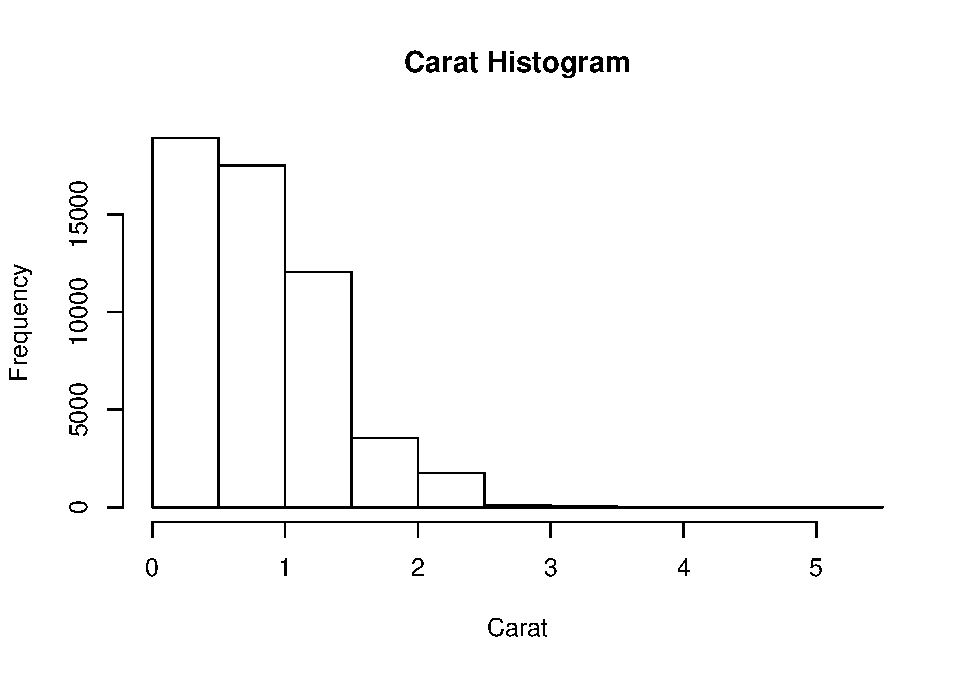
\includegraphics{Kor_BasicStats_files/figure-latex/unnamed-chunk-24-1.pdf}

\begin{Shaded}
\begin{Highlighting}[]
\CommentTok{## R애 내장된 기본 함수가 아니라 ggplot2를 이용해서 똑같은 히스토그램 만들어 보겠습니다.}
\KeywordTok{ggplot}\NormalTok{(}\DataTypeTok{data =}\NormalTok{ diamonds) }\OperatorTok{+}\StringTok{ }\KeywordTok{geom_histogram}\NormalTok{(}\KeywordTok{aes}\NormalTok{(}\DataTypeTok{x =}\NormalTok{ carat))}
\end{Highlighting}
\end{Shaded}

\begin{verbatim}
## `stat_bin()` using `bins = 30`. Pick better value with `binwidth`.
\end{verbatim}

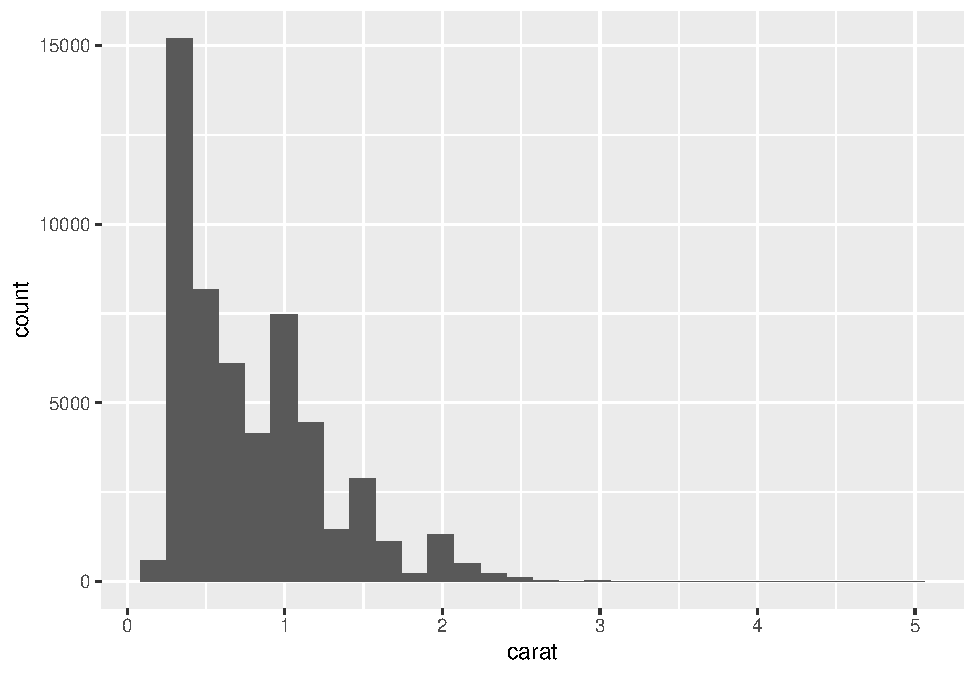
\includegraphics{Kor_BasicStats_files/figure-latex/unnamed-chunk-24-2.pdf}

\begin{Shaded}
\begin{Highlighting}[]
\CommentTok{## ggplot2는 "+"를 이용해서 다양한 형태의 추가적인 정보를 레이어 형식으로 더할 수 있습니다.}
\KeywordTok{ggplot}\NormalTok{(}\DataTypeTok{data =}\NormalTok{ diamonds) }\OperatorTok{+}\StringTok{ }
\StringTok{  }\KeywordTok{geom_histogram}\NormalTok{(}\KeywordTok{aes}\NormalTok{(}\DataTypeTok{x =}\NormalTok{ carat), }\DataTypeTok{fill =} \StringTok{"grey50"}\NormalTok{) }\OperatorTok{+}\StringTok{ }\CommentTok{# 히스토그램 막대색 변경}
\StringTok{  }\KeywordTok{ylab}\NormalTok{(}\StringTok{"Frequency"}\NormalTok{) }\OperatorTok{+}\StringTok{ }\KeywordTok{xlab}\NormalTok{(}\StringTok{"Carots"}\NormalTok{) }\OperatorTok{+}
\StringTok{  }\KeywordTok{ggtitle}\NormalTok{(}\StringTok{"Count of diamonds by size"}\NormalTok{) }\OperatorTok{+}
\StringTok{  }\KeywordTok{theme_bw}\NormalTok{() }\CommentTok{# 그래프 배경색 변경}
\end{Highlighting}
\end{Shaded}

\begin{verbatim}
## `stat_bin()` using `bins = 30`. Pick better value with `binwidth`.
\end{verbatim}

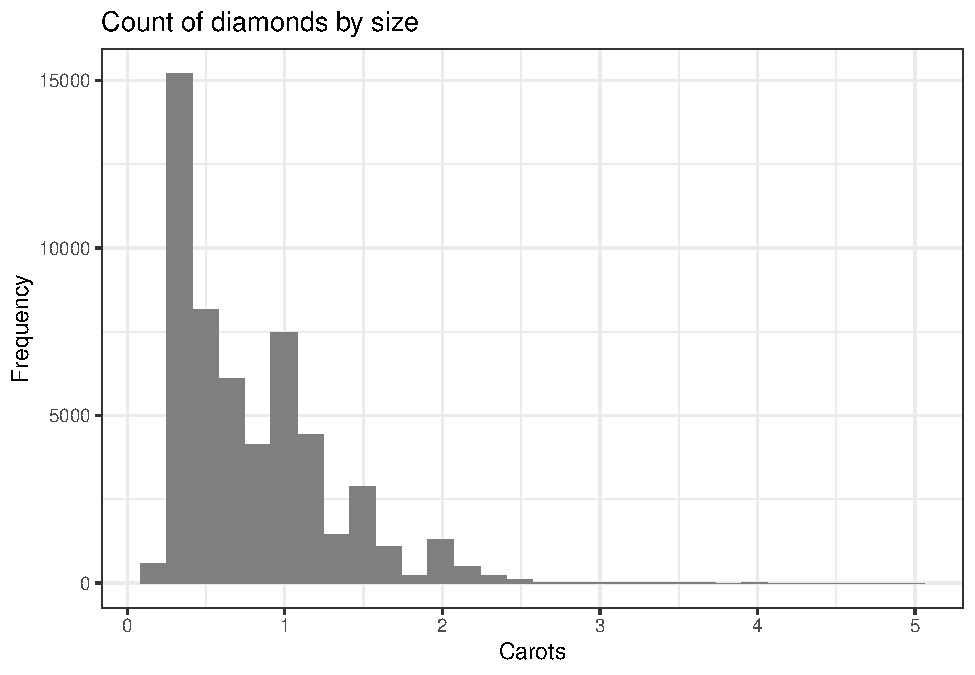
\includegraphics{Kor_BasicStats_files/figure-latex/unnamed-chunk-24-3.pdf}

\begin{Shaded}
\begin{Highlighting}[]
\CommentTok{## 아까 만들었던 그래프 폴더에 그래프를 저장할 수 있습니다.}
\CommentTok{# ggsave(file="./figures/figure1.pdf", width=6.5, height=5)}
\CommentTok{# ggsave(file="./figures/figure1a.png", width=6.5, height=5, device = "png")}
\end{Highlighting}
\end{Shaded}

\begin{Shaded}
\begin{Highlighting}[]
\CommentTok{## 표 폴더 만든 것에다가 요약통계표를 저장하기}
\KeywordTok{library}\NormalTok{(stargazer) }\CommentTok{# 통계표를 작성하는 데 특화된 패키지입니다.}

\CommentTok{## 세 가지 변수에 대해 요약통계치를 확인하기}
\NormalTok{diamonds <-}\StringTok{ }\KeywordTok{subset}\NormalTok{(diamonds, }\DataTypeTok{select =} \KeywordTok{c}\NormalTok{(}\StringTok{"carat"}\NormalTok{, }\StringTok{"depth"}\NormalTok{, }\StringTok{"price"}\NormalTok{))}
\CommentTok{## 몇몇 R 예제 데이터들은 티블로 저장되어 있지 않을 수 있습니다. }
\CommentTok{## 이 경우에는 자료를 먼저 티블 유형으로 바꿔주고 시작하는 게 좋습니다.}
\CommentTok{## 자료 유형을 확인하는 함수는 class(), 혹은 typeof()입니다.}
\CommentTok{## library(tidyverse) # 아까 불러왔지만, 여기서는 로드하지 않았다고 가정합시다.}
\KeywordTok{class}\NormalTok{(diamonds)}
\NormalTok{diamonds <-}\StringTok{ }\KeywordTok{as_tibble}\NormalTok{(diamonds)}
\NormalTok{sum.table1 <-}\StringTok{ }\KeywordTok{stargazer}\NormalTok{(diamonds, }
                      \DataTypeTok{covariate.labels=}\KeywordTok{c}\NormalTok{(}\StringTok{"Size (carats)"}\NormalTok{, }
                                         \StringTok{"Cut"}\NormalTok{, }\StringTok{"Color"}\NormalTok{, }
                                         \StringTok{"Clarity"}\NormalTok{), }
                                         \DataTypeTok{title =} \StringTok{"Summary stats for diamond data"}\NormalTok{, }
                                         \DataTypeTok{label =} \StringTok{"table:summary1"}\NormalTok{)}
\CommentTok{# write(x=sum.table1, file="./tables/Summary1.tex") # LaTex로 열고 편집할 수 있습니다.}
\end{Highlighting}
\end{Shaded}

\hypertarget{uxae30uxd0c0-uxcc38uxace0uxc790uxb8cc}{%
\section{기타 참고자료}\label{uxae30uxd0c0-uxcc38uxace0uxc790uxb8cc}}

여기서 정리한 \texttt{Introduction\ to\ R}의 내용은 모두 \href{https://www.datacamp.com/}{DataCamp}와 \texttt{R\ for\ Everyone}이라는 자료의 내용을 요약, 정리한 것입니다. 책(\texttt{R\ for\ Everyone;\ R4E1})이야 구매할 수밖에 없지만 \texttt{DataCamp} 사이트의 강의들 중에는 무료강의가 많으니까 한 번쯤 확인해보는 것도 큰 도움이 될 거라고 생각합니다.

RStudio 홈페이지도 두 개의 기초강의를 제공하는데, \href{https://rstudio.cloud/}{RStudio Cloud}에 가입하여 \texttt{Primers}를 클릭하면 됩니다. \texttt{Primers}에서 \texttt{Basics}를 선택하면 두 개 강의를 볼 수 있는데, \texttt{R-coding}에 도움이 되는 건 \texttt{Programming\ Basics\ Course}입니다.

\hypertarget{ch3}{%
\chapter{Introduction to Data}\label{ch3}}

여기에서는 자료를 관리하고 다루는 방법들에 대해 간단한 소개를 하고자 합니다. 구체적으로 다룰 내용들은 다음과 같습니다.

\begin{itemize}
\tightlist
\item
  무작위 추출 (Random draws)
\item
  루프 (Loops)
\item
  히스토그램 (Histograms)
\item
  표 (Tables)
\item
  벡터에서 요소들을 만들고, 계산하고, 추출하는 법 (Creating, summing, pulling elements from vectors)
\item
  분포와 확률에 따라 사고하는 법
\end{itemize}

먼저, 시작하기에 앞서서 작업 디렉토리 (Working Directory)를 설정할 필요가 있습니다.

\hypertarget{uxc791uxc5c5-uxb514uxb809uxd1a0uxb9ac-uxc124uxc815}{%
\section{작업 디렉토리 설정}\label{uxc791uxc5c5-uxb514uxb809uxd1a0uxb9ac-uxc124uxc815}}

기본적으로 \textbf{R}은 설치할 때, 기본 설정된 폴더에 이어서 작업을 진행합니다. 이 경우 기존에 만들어놓은 \texttt{R.data} (\textbf{R} 파일 확장자)들을 불러들여서 Global Environment에 사용하지 않을 데이터들이 쌓이게 됩니다. 그러면 현재 작업하여 저장한 새로운 객체들과 기존 디렉토리에 상존하는 데이터들이 혼재되어 헷갈릴 수 있습니다.

그리고 어차피 연구를 진행하면 해당 프로젝트에 따르는 폴더들을 만들어서 별개로 진행해야할 필요가 있기 때문에, 애초에 연구에 필요한 R.data를 만들 때 그 폴더에 만들고 작업 디렉토리도 설정하는 게 마음 편합니다.

그럼 일단 작업 디렉토리를 확인하고, 변경하는 코드를 살펴보겠습니다.

\begin{Shaded}
\begin{Highlighting}[]
\KeywordTok{getwd}\NormalTok{() }\CommentTok{#현재 R이 인식하고 있는 작업 디렉토리가 어딘지 알려준다.}
\KeywordTok{setwd}\NormalTok{(}\StringTok{"C:/Users/phere"}\NormalTok{) }\CommentTok{#원하는 장소로 디렉토리를 변경한다.}
\end{Highlighting}
\end{Shaded}

기서 주의해야 할 것은, 디렉토리 주소를 적을 때에는 반드시 \texttt{""} 기호를 사용해야 한다는 것입니다. 그리고 아마 윈도우 PC는 \texttt{/}로 디렉토리를 구분하는 반면에 MAC OS의 경우는 \texttt{\textbackslash{}}(back slash)를 사용하는 것으로 알고 있습니다.

나중에 한 번 다루긴 하겠지만 몇 가지 함수들의 경우에는 MAC에서는 오류가 안 생기는데 윈도우에서는 오류가 발생하는 것들이 있습니다. 그런 경우가 조금 번거로울 때가 있기는 한데, 그 이외에는 뭐 다 같은 컴퓨터에 같은 \textbf{R}이니 큰 불편함은 없다고 할 수 있습니다 (하지만 MAC 구매 뽐뿌가 오는 것은 사실입니다).

\begin{Shaded}
\begin{Highlighting}[]
\KeywordTok{dir.create}\NormalTok{(}\DataTypeTok{path=} \StringTok{"figures"}\NormalTok{)}
\KeywordTok{dir.create}\NormalTok{(}\DataTypeTok{path=} \StringTok{"tables"}\NormalTok{)}
\KeywordTok{dir.create}\NormalTok{(}\DataTypeTok{path=} \StringTok{"datasets"}\NormalTok{)}
\KeywordTok{dir.create}\NormalTok{(}\DataTypeTok{path=} \StringTok{"references"}\NormalTok{)}
\KeywordTok{dir.create}\NormalTok{(}\DataTypeTok{path=} \StringTok{"tex"}\NormalTok{)}
\end{Highlighting}
\end{Shaded}

저 같은 경우에는 어떤 연구 프로젝트를 시작할 때, 제일 먼저 R-script 빈 것을 만들어두고 작업 디렉토리를 설정합니다.

\begin{itemize}
\tightlist
\item
  이후에 위의 코드와 같이 세부 폴더들을 만듭니다.
\item
  \textbf{R}로 만든 그래프들을 저장할 \texttt{figures}, 표를 저장할 \texttt{tables}, 기타 다운받은 데이터들을 저장할 \texttt{datasets}, 그리고 참고문헌을 저장할 \texttt{references}와 본문 작성을 위한 \texttt{tex} 폴더로 구성됩니다.
\end{itemize}

\hypertarget{uxbb34uxc791uxc704-uxcd94uxcd9crandom-draws}{%
\section{무작위 추출(Random Draws)}\label{uxbb34uxc791uxc704-uxcd94uxcd9crandom-draws}}

무작위 추출을 실제로 해보기 위해서 한 가지 시뮬레이션을 돌려 보겠습니다. 어떤 사업장에서 사람을 승진시키는 데 있어서 성차별(gender discrimination)이 있을 수 있다고 가정하는 것입니다. 간단하게 100명의 승진 후보자들이 있다고 가정하고, 남녀가 동일한 비율로 나뉘어져 있다고 생각해 보겠습니다. 그리고 일반적으로 승진할 확률은 70\% (0.7)라고 가정합니다. R-code로 남녀 각각 50명을 대상으로, 승진할 경우 1로 코딩하고 승진하지 못할 경우를 0으로 코딩하는 일종의 더미변수를 만들겠습니다. 그리고 승진 확률은 70\%로 설정합니다.

\begin{itemize}
\item
  즉, 무작위로 추출한 50명 중 승진확률이 그대로 반영된다면 우리는 35개의 1과 15개의 0을 확인할 수 있을 것입니다.
\item
  그러나 표본추출과 무작위화의 본연의 속성 상, 항상 확률대로 정확하게 그러한 비율의 결과를 갖는 것은 불가능합니다.
\item
  따라서 우리는 무작위로 추출할 때마다 약 70\% 승진확률에 근거한 그 언저리의 값들을 얻게 될 것입니다.

\begin{Shaded}
\begin{Highlighting}[]
\NormalTok{MP <-}\StringTok{ }\KeywordTok{rbinom}\NormalTok{(}\DecValTok{50}\NormalTok{, }\DecValTok{1}\NormalTok{, }\FloatTok{.7}\NormalTok{) }\CommentTok{#70%의 승진확률로 무작위로 추출한 50명의 남성}
\NormalTok{WP <-}\StringTok{ }\KeywordTok{rbinom}\NormalTok{(}\DecValTok{50}\NormalTok{, }\DecValTok{1}\NormalTok{, }\FloatTok{.7}\NormalTok{) }\CommentTok{#70%의 승진확률로 무작위로 추출한 50명의 여성}
\KeywordTok{sum}\NormalTok{(MP) }\CommentTok{#총 승진한 남성의 수}
\end{Highlighting}
\end{Shaded}

\begin{verbatim}
## [1] 35
\end{verbatim}

\begin{Shaded}
\begin{Highlighting}[]
\KeywordTok{sum}\NormalTok{(WP) }\CommentTok{#총 승진한 여성의 수}
\end{Highlighting}
\end{Shaded}

\begin{verbatim}
## [1] 37
\end{verbatim}

\begin{Shaded}
\begin{Highlighting}[]
\KeywordTok{sum}\NormalTok{(MP)}\OperatorTok{/}\DecValTok{50} \CommentTok{#전체 남성 승진후보자에 대한 승진한 남성의 비율}
\end{Highlighting}
\end{Shaded}

\begin{verbatim}
## [1] 0.7
\end{verbatim}

\begin{Shaded}
\begin{Highlighting}[]
\KeywordTok{sum}\NormalTok{(WP)}\OperatorTok{/}\DecValTok{50} \CommentTok{#전체 여성 승진후보자에 대한 승진한 여성의 비율}
\end{Highlighting}
\end{Shaded}

\begin{verbatim}
## [1] 0.74
\end{verbatim}
\end{itemize}

\texttt{MP}와 \texttt{WP}는 각각 Mem Promotion과 Women Promotion의 약자입니다. \texttt{rbinom()}은 randomly draw as binomial로 이해하면 됩니다. 따라서 이 함수의 뜻은 ``50개의 이항변수를 만드는 데 1의 값을 가질 확률을 0.7로 해서 추출해라''고 할 수 있겠습니다.\footnote{자세한 내용은 Kachitvichyanukul, V. and Schmeiser, B. W. (1988) ``Binomial random variate generation.'' \emph{Communications of the ACM}, 31, 216--222.를 참조. \texttt{?rbinom}이라고 R-console에 입력하면 우측 하단의 창에서 함수들에 대한 자세한 설명을 볼 수 있습니다.}

이렇게 만든 \texttt{MP}와 \texttt{WP}에 1, 즉 승진자가 각각 몇명인지 살펴보려면 단순하게 \texttt{sum()}, 합계를 나타내는 함수를 이용하면 됩니다. \texttt{MP}와 \texttt{WP}는 각각 벡터 자료로 값을 가지는데, \texttt{sum()}을 이용하면 이 벡터 자료의 각 요소들(elements)의 합을 계산할 수 있습니다. 만약 실제로 관측된 50명 각각에 대한 승진확률을 구하려면 그 집단의 총 인원수로 나누면 됩니다.

우리가 알고 싶은 것은 과연 이 사업장에서 승진하는 데 남녀의 성차별이 있느냐는 것입니다.

\begin{itemize}
\tightlist
\item
  다시 말하면 남자와 여자의 승진 결과에 있어서 어떤 차이가 나타날 수는 있는데, 과연 그 차이가 진짜로 차별이 있어서 나타나는지를 확인하자는 것입니다.
\item
  이를 위해서 우리는 주어진 표본(남녀 각 50명, 총 100명에 있어서의)에서의 승진자 수의 차이를 계산해야 합니다.
\end{itemize}

\begin{Shaded}
\begin{Highlighting}[]
\NormalTok{DP <-}\StringTok{ }\KeywordTok{sum}\NormalTok{(MP) }\OperatorTok{-}\StringTok{ }\KeywordTok{sum}\NormalTok{(WP) }\CommentTok{#DP는 Difference in Promotion, 승진자 수의 차이입니다.}
\end{Highlighting}
\end{Shaded}

\texttt{DP}의 값이 양수(positive)라면 남성 승진자의 수가 더 많다는 의미일 것이고, 음수(negative)라면 여성 승진자의 수가 더 많다고 볼 수 있습니다. 만약 \texttt{DP}가 0이면 두 성별에서의 승진자의 수가 동일하다는 것입니다다. 우리는 \textbf{R}을 이용하여 이와 같은 표집(sampling)을 여러 번 시뮬레이션 해볼 수 있습니다.

앞선 100명(남50 여50)을 추출한 것을 말 그대로 여러 번 반복할 수 있다는 것인데, 50명에 대한 확률은 0.7로 동일하더라도 무작위 추출이기 때문에 매번 추출할 때마다 그 결과는 달라질 것입니다.

\begin{itemize}
\tightlist
\item
  우리가 알고 싶은 것은 이렇게 여러 번 추출해서 돌리더라도 만약 성차별이 실제로 존재한다면 꾸준하게, 그리고 일정한 차이로 \texttt{DP}가 나타날 것이라는 점입니다.
\item
  만약 \texttt{DP}가 있다가 없다가 한다면 통계적 관점으로 ``평균적으로'' (on average) 그 효과는 체계적이지 않을(non-systematic) 가능성이 높습니다.
\end{itemize}

먼저, 10개의 결측치를 가진 벡터를 만들어보겠습니다. 이게 무슨 말이냐면 아무 값도 들어있지 않은 10개 열자리 1개 행의 표를 만들라는 얘기로 이해할 수 있습니다. 완전 같은 말은 아닌데, 뭐 이렇게 이해하면 편할 거 같습니다. 그리고 그 각각의 칸에 이제부터 총 10번 시뮬레이팅하여 남50 여50에 대한 승진자 수의 차이 값 10개를 채워넣겠습니다.

\begin{Shaded}
\begin{Highlighting}[]
\NormalTok{trial.size <-}\StringTok{ }\DecValTok{10} \CommentTok{#시뮬레이션을 시도할 횟수}
\NormalTok{Test10 <-}\StringTok{ }\KeywordTok{rep}\NormalTok{(}\OtherTok{NA}\NormalTok{, trial.size) }\CommentTok{##rep는 replicate, 즉 반복하라는 함수입니다.}
                              \CommentTok{##즉, 이 함수는 trial.size의 수만큼 NA를 반복해서}
                              \CommentTok{##Test10이라는 벡터에 담으라는 의미입니다.}
\NormalTok{Test10 }\CommentTok{#위의 함수를 통해 얻게 되는 Test10 벡터의 값은 아래와 같습니다.}
\end{Highlighting}
\end{Shaded}

\begin{verbatim}
##  [1] NA NA NA NA NA NA NA NA NA NA
\end{verbatim}

그리고 나서 우리는 이 10칸의 NA, 결측치(missing values)에 10번에 시뮬레이션을 통해 얻은 승진자 수의 차이(총 10개의 차이)를 담을 것입니다. 귀찮게 함수를 10번 반복할 수도 있겠지만, 만약 시뮬레이션을 해야 하는 수가 10번이 아니라 100만 번이라면 그 짓하다가 하루? 일주일이 다 갈 것이기 때문에 여기서부터 루프 (Loops)를 알아봅시다.

\hypertarget{uxb8e8uxd504-uxbc18uxbcf5loops}{%
\section{루프-반복(Loops)}\label{uxb8e8uxd504-uxbc18uxbcf5loops}}

자, 10번 반복하기를 해보겠습니다. 함수는 아래와 같습니다.

\begin{Shaded}
\begin{Highlighting}[]
\ControlFlowTok{for}\NormalTok{ (a }\ControlFlowTok{in} \DecValTok{1}\OperatorTok{:}\NormalTok{trial.size) \{ }\CommentTok{# a라는 벡터에 1부터 trial.size까지의 수를 넣으라는 명령}
\NormalTok{  MP <-}\StringTok{ }\KeywordTok{rbinom}\NormalTok{(}\DecValTok{50}\NormalTok{, }\DecValTok{1}\NormalTok{, }\FloatTok{.7}\NormalTok{) }\CommentTok{# MP를 계산하라, 총 50명이 0.7의 확률로 1을 가질 것}
\NormalTok{  WP <-}\StringTok{ }\KeywordTok{rbinom}\NormalTok{(}\DecValTok{50}\NormalTok{, }\DecValTok{1}\NormalTok{, }\FloatTok{.7}\NormalTok{) }\CommentTok{# WP를 계산하라, 총 50명이 0.7의 확률로 1을 가질 것}
\NormalTok{  Test10[a] <-}\StringTok{ }\NormalTok{(}\KeywordTok{sum}\NormalTok{(MP) }\OperatorTok{-}\StringTok{ }\KeywordTok{sum}\NormalTok{(WP))}\OperatorTok{/}\DecValTok{50}
\NormalTok{\}}
\end{Highlighting}
\end{Shaded}

위의 함수를 통해서 우리는 총 10개의 \texttt{DP}값을 50으로 나눈, 승진자 수의 차이가 한 개 집단에(남 or 녀) 대해 비율로 계산된 벡터의 형식으로 \texttt{Test10}에 가지게 됩니다. \texttt{Test10{[}1{]}}은 첫 번째 시뮬레이션의 \texttt{DP} 확률이고 \texttt{Test10{[}4{]}}는 네 번째 시뮬레이션의 \texttt{DP} 확률을 가지게 될 것입니다. 벡터 자료 뒤에 \texttt{{[}n{]}}는 그 벡터의 \texttt{n}번째 요소를 보여달라는 명령입니다.

\begin{Shaded}
\begin{Highlighting}[]
\KeywordTok{hist}\NormalTok{(Test10)}
\end{Highlighting}
\end{Shaded}

\begin{center}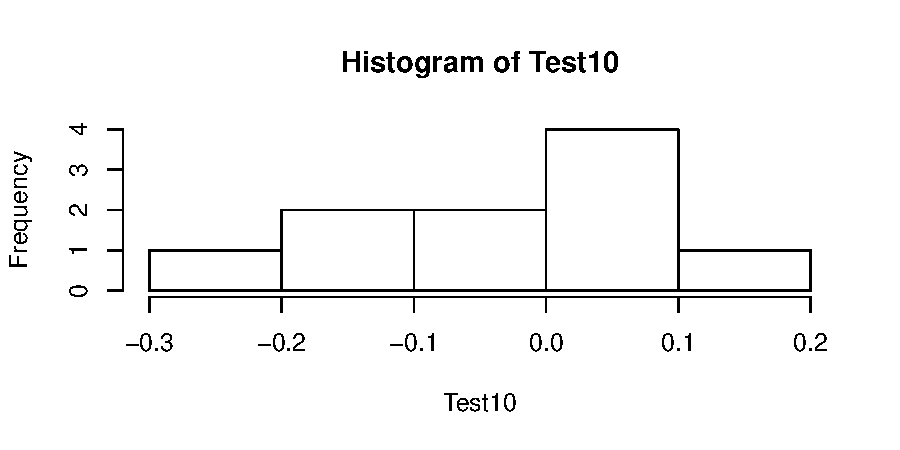
\includegraphics{Kor_BasicStats_files/figure-latex/unnamed-chunk-33-1} \end{center}

총 10개의 \texttt{Test10}의 값을 구해 히스토그램을 구한 것입니다. 즉, 10개 \texttt{DP} 확률의 분포를 나타낸 것이라고 할 수 있습니다. 10개의 표본으로는 뚜렷한 경향을 보기가 힘듭니다. 한 번 백 개의 시뮬레이션을 진행해보겠습니다. 진행과정은 10번의 시뮬레이션이랑 동일합니다. 단지 \texttt{trial.size}가 100으로 늘어났다는 것과 반복횟수가 \texttt{b}로 \texttt{a}랑 구분한다는 것만 다릅니다.

\begin{Shaded}
\begin{Highlighting}[]
\NormalTok{trial.size <-}\StringTok{ }\DecValTok{100}
\NormalTok{Test100 <-}\StringTok{ }\KeywordTok{rep}\NormalTok{(}\OtherTok{NA}\NormalTok{, trial.size)}
\ControlFlowTok{for}\NormalTok{ (b }\ControlFlowTok{in} \DecValTok{1}\OperatorTok{:}\NormalTok{trial.size) \{}
\NormalTok{  MP <-}\StringTok{ }\KeywordTok{rbinom}\NormalTok{(}\DecValTok{50}\NormalTok{, }\DecValTok{1}\NormalTok{, }\FloatTok{.7}\NormalTok{)}
\NormalTok{  WP <-}\StringTok{ }\KeywordTok{rbinom}\NormalTok{(}\DecValTok{50}\NormalTok{, }\DecValTok{1}\NormalTok{, }\FloatTok{.7}\NormalTok{)}
\NormalTok{  Test100[b] <-}\StringTok{ }\NormalTok{(}\KeywordTok{sum}\NormalTok{(MP) }\OperatorTok{-}\StringTok{ }\KeywordTok{sum}\NormalTok{(WP))}\OperatorTok{/}\DecValTok{50}
\NormalTok{\}}
\KeywordTok{hist}\NormalTok{(Test100)}
\end{Highlighting}
\end{Shaded}

\begin{center}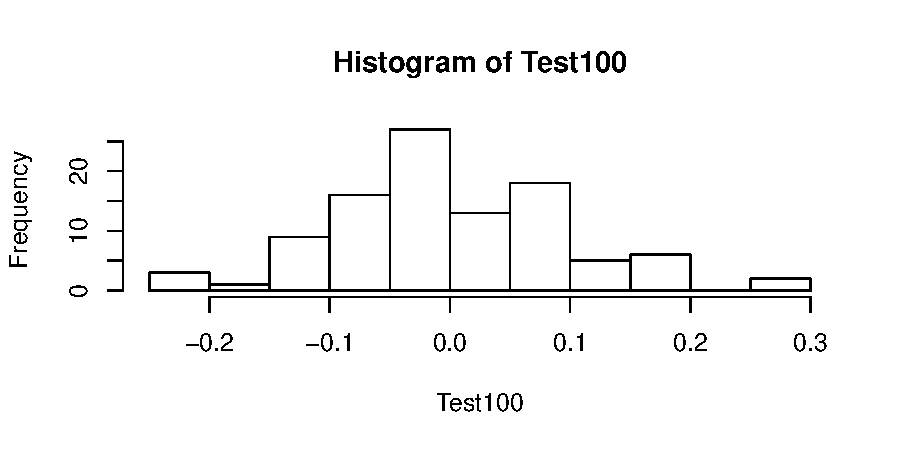
\includegraphics{Kor_BasicStats_files/figure-latex/unnamed-chunk-34-1} \end{center}

매우 눈에 익숙하고 우리가 사랑하는(?) 분포의 형태로 변해가는 것을 볼 수 있습니다. 이제 극단적으로 백 만번의 시뮬레이션을 진행해보겠습니다.

\begin{Shaded}
\begin{Highlighting}[]
\NormalTok{trial.size3 <-}\StringTok{ }\DecValTok{1000000}
\NormalTok{Test1M <-}\StringTok{ }\KeywordTok{rep}\NormalTok{(}\OtherTok{NA}\NormalTok{, trial.size3)}
\ControlFlowTok{for}\NormalTok{ (c }\ControlFlowTok{in} \DecValTok{1}\OperatorTok{:}\NormalTok{trial.size3) \{}
\NormalTok{  MP <-}\StringTok{ }\KeywordTok{rbinom}\NormalTok{(}\DecValTok{50}\NormalTok{, }\DecValTok{1}\NormalTok{, }\FloatTok{.7}\NormalTok{)}
\NormalTok{  WP <-}\StringTok{ }\KeywordTok{rbinom}\NormalTok{(}\DecValTok{50}\NormalTok{, }\DecValTok{1}\NormalTok{, }\FloatTok{.7}\NormalTok{)}
\NormalTok{  Test1M[c] <-}\StringTok{ }\NormalTok{(}\KeywordTok{sum}\NormalTok{(MP) }\OperatorTok{-}\StringTok{ }\KeywordTok{sum}\NormalTok{(WP))}\OperatorTok{/}\DecValTok{50}
\NormalTok{\}}
\KeywordTok{hist}\NormalTok{(Test1M)}
\end{Highlighting}
\end{Shaded}

\begin{center}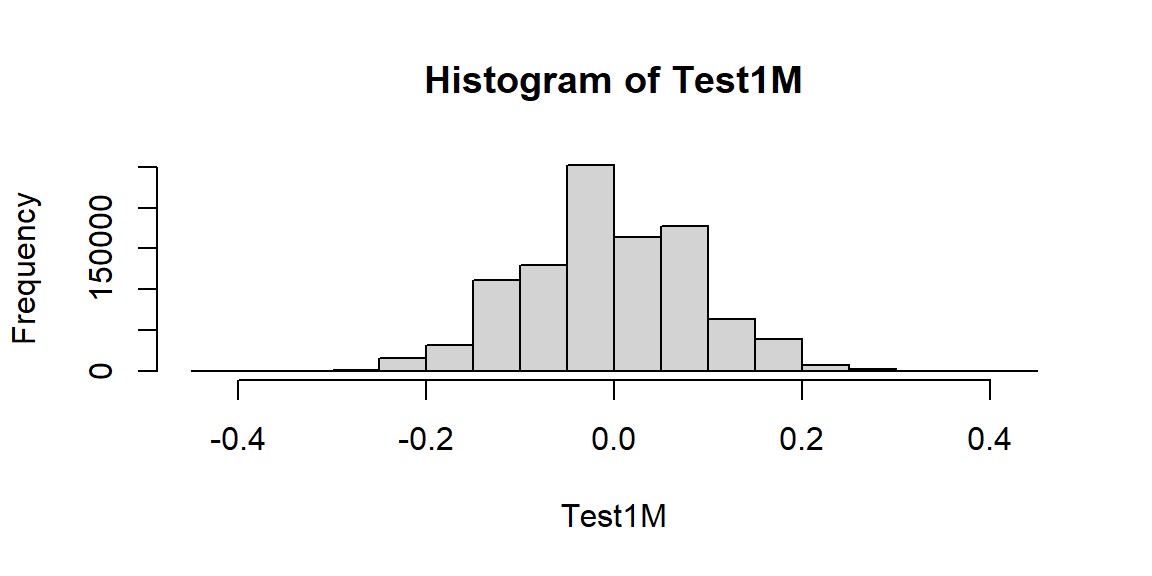
\includegraphics{Kor_BasicStats_files/figure-latex/unnamed-chunk-35-1} \end{center}

여기서 한 가지 알 수 있는 것은 시뮬레이션 시도 횟수가 늘어날수록(무한에 가까워질수록), 우리가 알고 싶어하는 승진에서의 차이(결과)의 진짜 확률(true probabilities)이 드러난다는 것입니다.

\begin{itemize}
\tightlist
\item
  이는 나중에 표집(sampling)과 표집오차(sampling errors), 그리고 중심극한정리(Central Limit Theorem)을 언급할 일이 있을 때 다시 살펴보도록 하겠습니다.
\end{itemize}

위에서 추출한 100만번의 시뮬레이션 결과를 토대로 남성과 여성의 승진에 있어서의 차이가 과연 0.3보다 큰지 살펴보겠습니다.

\begin{itemize}
\item
  조금 더 문제를 단순화하기 위해서 남자가 여성보다 더 승진할 가능성, 승진자 수의 차이가 전체 후보자에 대한 비율에 있어서 +0.3보다 큰지 작은지를 살펴보려는 것입니다.
\item
  먼저 각각(남성과 여성)에 있어서의 승진자 수의 차이를 비율로 구하여 그 비율이 0.3보다 크거나 같은 경우가 전체 시뮬레이션으로 나타난 승진자 수의 차이 비율 전체의 몇 퍼센트를 차지하는지 구합니다.

\begin{Shaded}
\begin{Highlighting}[]
\KeywordTok{length}\NormalTok{(Test1M[Test1M }\OperatorTok{>=}\StringTok{ }\FloatTok{0.3}\NormalTok{]) }\OperatorTok{/}\StringTok{ }\KeywordTok{length}\NormalTok{(Test1M)}
\end{Highlighting}
\end{Shaded}

\begin{verbatim}
## [1] 0.000732
\end{verbatim}
\item
  처음에 R을 할 때 잘 외우지 못했던 함수 중 하나인데, \texttt{length()}는 뭐랄까\ldots{} \texttt{count}라고 이해하면 조금 더 쉬울 것 같습니다.\footnote{나중에 가면 알아볼 \texttt{dplyr} 패키지에는 그룹별 관측치의 개수를 셀 수 있는 \texttt{count()} 함수가 존재합니다.}
\item
  즉, 아래의 함수는 \texttt{Test1M}, 100만개의 승진자 수가 전체 집단에서 차지하는 비율이 0.3보다 큰 경우만을 구해서 그걸 전체 승진차이 확률 100만개에 대한 비율로 구하라는 것입니다.

  \begin{itemize}
  \tightlist
  \item
    남자가 여자에 비해서 30\% 이상 승진을 많이 할 확률이 나타난 것이 총 100만번의 시뮬레이션 가운데 몇 번이었냐는 것입니다.
  \end{itemize}
\item
  아래 함수는 그 결과는 0.000711, 즉 약 0.07\%의 확률로 남자가 여자에 비해 30\% 이상 승진자가 많을 확률이 나타난다는 것을 알 수 있습니다.
\item
  적어도 이 예제에 한하여 해석은 개인의 몫으로 남겨 놓겠습니다.
\end{itemize}

\hypertarget{rplotsuxb97c-uxd30cuxc77cuxc758-uxd615uxd0dcuxb85c-uxc800uxc7a5uxd558uxae30}{%
\section{Rplots를 파일의 형태로 저장하기}\label{rplotsuxb97c-uxd30cuxc77cuxc758-uxd615uxd0dcuxb85c-uxc800uxc7a5uxd558uxae30}}

이번 섹션에는 조금 기술적인(technical) 소개를 하고자 합니다. 바로 위에서 만든 히스토그램 등을 \texttt{pdf}나 \texttt{png}와 같은 형태의 파일로 저장하는 함수입니다. 먼저 \texttt{pdf}로 저장하는 것을 살펴보겠습니다. \texttt{pdf}로 저장하는 것은 추천할만한 방식입니다. \LaTeX를 이용하는 경우에는 이렇게 저장한 pdf를 깔끔하게 \LaTeX로 생산하는 pdf 문서에 삽입할 수 있습니다.

\begin{Shaded}
\begin{Highlighting}[]
\KeywordTok{pdf}\NormalTok{(}\StringTok{"figures/histogram.pdf"}\NormalTok{, }\DataTypeTok{width=}\DecValTok{8}\NormalTok{, }\DataTypeTok{height=}\DecValTok{6}\NormalTok{) }
\CommentTok{## 아까 만든 figures에 histogram.pdf라는 이름으로 저장하게 합니다.}
\KeywordTok{hist}\NormalTok{(Test1M, }\DataTypeTok{xlab =} \StringTok{"Margin"}\NormalTok{, }\DataTypeTok{main =} \OtherTok{NULL}\NormalTok{)  }\CommentTok{#표 전체 제목은 NULL, 없습니다}
\CommentTok{##Test1M, 100만번 시뮬레이팅한 히스토그램 X축에는 Margin이라고 레이블을 달 것입니다.}
\KeywordTok{dev.off}\NormalTok{()}
\end{Highlighting}
\end{Shaded}

\texttt{dev.off}는 \texttt{device\ off}로 위의 함수는 여기서 끝!이라고 이해하시면 되겠습니다다.자세한 내용은 \texttt{?dev.off}로 알아보시길\ldots{} 그리고 pdf로 저장하기 어려운 경우에는 png로 저장할 경우 해상도 자체는 조금 떨어지지만 유용하게 쓸 수 있는 그림파일로 동일한 Rplots를 저장할 수 있습니다. pdf는 인치(Inches)로 저장되는데, png는 픽셀(Pixels)로 저장됩니다. 그래서 아래 코드에서의 너비랑 높이를 지정하는 방법이 조금 다릅니다.

\begin{Shaded}
\begin{Highlighting}[]
\KeywordTok{png}\NormalTok{(}\StringTok{"figures/histogram.png"}\NormalTok{, }\DataTypeTok{width=}\DecValTok{720}\NormalTok{, }\DataTypeTok{height=}\DecValTok{480}\NormalTok{)}
\KeywordTok{hist}\NormalTok{(Test1M, }\DataTypeTok{xlab =} \StringTok{"Margin"}\NormalTok{, }\DataTypeTok{main =} \OtherTok{NULL}\NormalTok{)}
\KeywordTok{dev.off}\NormalTok{()}
\end{Highlighting}
\end{Shaded}

\hypertarget{uxb370uxc774uxd130-uxb2e4uxb8e8uxae30-uxae30uxbcf8}{%
\section{데이터 다루기 기본}\label{uxb370uxc774uxd130-uxb2e4uxb8e8uxae30-uxae30uxbcf8}}

이번 섹션부터는 데이터에 대해 조금 더 깊이 살펴보고자 합니다. 구체적으로는,

\begin{itemize}
\tightlist
\item
  데이터 불러오기 (loading)
\item
  서로 다른 분석수준, 분석단위를 가지고 작업하기 (working with different levels of analysis/units of observation)
\item
  작업 흐름(workflow)
\end{itemize}

순으로 진행하고자 합니다.

먼저 기존에 존재하던 데이터셋을 불러오기에 앞서 개략적으로 데이터라는 것이 어떻게 생겼는지를 살펴볼 필요가 있습니다. 데이터프레임은 열에 변수(variables), 행에 관측치들을 갖는 형태로 이루어져 있습니다. 하지만 앞서 언급했던 바와 같이, 데이터프레임 유형보다는 티블을 사용하는 것이 앞으로 배울 함수들을 적용하기에 좀 더 효율적입니다. 따라서 티블 함수를 이용해 가상의 데이터셋을 직접 만들어 보겠습니다.

\begin{Shaded}
\begin{Highlighting}[]
\KeywordTok{library}\NormalTok{(tidyverse) }\CommentTok{# 티블을 사용하기 위해서는 tidyverse 패키지를 불러와줘야 합니다.}
\NormalTok{data1 <-}\StringTok{ }\KeywordTok{tibble}\NormalTok{(}\DataTypeTok{name =} \KeywordTok{c}\NormalTok{(}\StringTok{"Jane"}\NormalTok{, }\StringTok{"John"}\NormalTok{, }\StringTok{"Jen"}\NormalTok{, }\StringTok{"James"}\NormalTok{),}
                \DataTypeTok{height =} \KeywordTok{c}\NormalTok{(}\DecValTok{60}\NormalTok{, }\DecValTok{70}\NormalTok{, }\DecValTok{65}\NormalTok{, }\DecValTok{68}\NormalTok{),}
                \DataTypeTok{eye.color =} \KeywordTok{c}\NormalTok{(}\StringTok{"blue"}\NormalTok{, }\StringTok{"blue"}\NormalTok{, }\StringTok{"brown"}\NormalTok{, }\StringTok{"brown"}\NormalTok{),}
                \DataTypeTok{gender =} \KeywordTok{c}\NormalTok{(}\StringTok{"female"}\NormalTok{, }\StringTok{"male"}\NormalTok{, }\StringTok{"female"}\NormalTok{, }\StringTok{"male"}\NormalTok{),}
                \DataTypeTok{highest.degree =} \KeywordTok{c}\NormalTok{(}\StringTok{"college"}\NormalTok{, }
                                   \StringTok{"high school"}\NormalTok{, }
                                   \StringTok{"post graduate"}\NormalTok{, }
                                   \StringTok{"college"}\NormalTok{))}
\KeywordTok{glimpse}\NormalTok{(data1)}
\end{Highlighting}
\end{Shaded}

\begin{verbatim}
## Observations: 4
## Variables: 5
## $ name           <chr> "Jane", "John", "Jen", "James"
## $ height         <dbl> 60, 70, 65, 68
## $ eye.color      <chr> "blue", "blue", "brown", "brown"
## $ gender         <chr> "female", "male", "female", "male"
## $ highest.degree <chr> "college", "high school", "post graduate", "col...
\end{verbatim}

만약 티블이 아니라 데이터프레임으로 저장하고 싶으시다면 \texttt{tibble()} 대신 \texttt{data.frame()} 함수를 사용하시면 됩니다. 이렇게 생성된 데이터는 열(column)에 변수를 갖습니다.

\begin{itemize}
\tightlist
\item
  \texttt{data1}에서는 \texttt{name,\ height,\ eye.color,\ gender,\ highest.degree}가 변수명이 됩니다.
\item
  그리고 각 변수의 하위에 행마다 관측치들이 주어집니다다.

  \begin{itemize}
  \tightlist
  \item
    \texttt{name}이라는 변수에는 \texttt{Jane,\ John,\ Jen,\ James} 라는 각 개인을 관측한 결과가 입력됩니다다.
  \item
    \texttt{c()}는 안의 요소들을 벡터의 형태로 묶으라는 것입니다(이전 포스팅에서 벡터에 대한 설명 참조).
  \end{itemize}
\item
  그리고 이렇게 만들어진 데이터의 구조를 확인하기 위해서는 \texttt{glimpse()} 함수를 사용하면 된다.

  \begin{itemize}
  \tightlist
  \item
    \texttt{str()} 함수도 있는데, \texttt{glimpse()}가 좀 더 깔끔하게 데이터의 구조를 보여주는 것 같습니다.
  \end{itemize}
\end{itemize}

\hypertarget{uxb370uxc774uxd130uxc5d0-uxc0c8uxb85cuxc6b4-uxbcc0uxc218-uxb354uxbbf8uxbcc0uxc218-uxb9ccuxb4e4uxae30}{%
\subsection{데이터에 새로운 변수 \& 더미변수 만들기}\label{uxb370uxc774uxd130uxc5d0-uxc0c8uxb85cuxc6b4-uxbcc0uxc218-uxb354uxbbf8uxbcc0uxc218-uxb9ccuxb4e4uxae30}}

기존 데이터에 새로운 변수를 추가하는 방법은 매우 간단합니다. 그냥 새로운 변수명을 \texttt{\$} 표시를 이용해 데이터에 써주고 거기에 배정(assign)을 의미하는 \texttt{\textless{}-} 표시로 넣어주면 됩니다. 백문이 불여일견이니 한 번 해보겠습니다.

\begin{Shaded}
\begin{Highlighting}[]
\NormalTok{data1}\OperatorTok{$}\NormalTok{female <-}\StringTok{ }\OtherTok{NA}
\end{Highlighting}
\end{Shaded}

위의 코드는 \texttt{female}이라는 변수를 새롭게 만들되 \texttt{female}의 모든 관측치는 결측치(missing values)로 생성하라는 것을 의미합니다.우측 항에 단순한 값을 적는다면 데이터의 새로운 변수, 일종의 벡터에는 모두 그 값으로 채워질 것입니다. 반면, 우리가 원하는 체계적인 형태의 변수(\texttt{var}iable)로 대체하고 싶다면 함수(function)를 이용하면 됩니다.

여기서 살펴볼 더미변수란 말 그대로 더미(dummy), 바보 변수입니다. 더미변수는 존부(存否)만을 나타내는 변수인데 \texttt{1}일 경우에는 있음, \texttt{0}일 경우에는 없음을 나타냅니다. 예를 들어, 바로 아래에서 만들 \texttt{female}변수는 여성일 경우에 \texttt{1}, 남성일 경우에 \texttt{0}을 나타낼 것입니다. 아까 만든 데이터(\texttt{data1})의 변수 중 \texttt{gender}는 남성(\texttt{male})과 여성(\texttt{female})이라는 두 문자열 변수로 구성되어 있는데, 이를 숫자형(numerical)으로 바꿔주고자 하는 것입니다.

더미변수는 어떤 점에서는 유용하지만 존부 이외의 자세한 정보를 제공하지 못한다는 점에서 더미라고 불립니다. 일단, 더미변수(숫자형)으로서의 여성(사실상 성별) 변수를 추가해보겠습니다.

\begin{Shaded}
\begin{Highlighting}[]
\NormalTok{data1}\OperatorTok{$}\NormalTok{female <-}\StringTok{ }\KeywordTok{ifelse}\NormalTok{(data1}\OperatorTok{$}\NormalTok{gender }\OperatorTok{==}\StringTok{ "female"}\NormalTok{, }\DecValTok{1}\NormalTok{, }\DecValTok{0}\NormalTok{)}
\CommentTok{## 해석: data1에 female이라는 변수에 우측 함수에 따른 값을 배정하라.}
\CommentTok{##      ifelse(만약 ~ 면, A를, ~가 아니라면, B를) 배정하라.}
\CommentTok{## 따라서 위의 함수는 data1의 gender 변수가 "female"이라는 문자일 경우 새로운 female}
\CommentTok{## 변수에 1을, "female"이 아닌 경우에는 0을 주어라.}
\NormalTok{data1}\OperatorTok{$}\NormalTok{female }\CommentTok{# 더미 변수의 이름을 지을 때에는 기준값(reference value)이 헷갈리지 않게}
\end{Highlighting}
\end{Shaded}

\begin{verbatim}
## [1] 1 0 1 0
\end{verbatim}

\begin{Shaded}
\begin{Highlighting}[]
             \CommentTok{# 1의 값을 갖는 라벨(label)로 변수 이름을 짓는게 좋다 (TIP)}
\NormalTok{data1}\OperatorTok{$}\NormalTok{gender <-}\StringTok{ }\OtherTok{NULL} \CommentTok{# 이제 사용하지 않을 gender 변수는 결측치로 변경.}
\end{Highlighting}
\end{Shaded}

그리고 한 가지 짚고 넘어갈 것은 \textbf{R}에서는 요인형(factor)과 문자형(character) 유형이 다르다는 것입니다. 요인형 자료를 문자형 자료로 변환하거나 혹은 그 역도 가능하지만 요인형에서 문자형으로 변환하는 것은 별로 추천드리고 싶지 않습니다. 일단 기본적으로 이 내용은 일반적인 통계분석을 다루고 있기 때문에 문자형 그 자체를 가지고 뭔가를 분석하는 텍스트 분석이 아닌 이상 문자열은 그저 고유값, 이상도 이하도 아니기 때문입니다. 하나 밖에 없는 값으로 무언가를 일반화하거나 설명하기란 쉽지 않습니다.

\begin{Shaded}
\begin{Highlighting}[]
\NormalTok{data1}\OperatorTok{$}\NormalTok{name <-}\StringTok{ }\KeywordTok{as.character}\NormalTok{(data1}\OperatorTok{$}\NormalTok{name) }
\CommentTok{# name 변수의 자료들은 문자형(STATA에서 string이라고 하는)으로 이루어져 있는데, }
\CommentTok{# 이를 요인형으로 바꾸는 것이다.}
\KeywordTok{glimpse}\NormalTok{(data1)}
\end{Highlighting}
\end{Shaded}

\begin{verbatim}
## Observations: 4
## Variables: 5
## $ name           <chr> "Jane", "John", "Jen", "James"
## $ height         <dbl> 60, 70, 65, 68
## $ eye.color      <chr> "blue", "blue", "brown", "brown"
## $ highest.degree <chr> "college", "high school", "post graduate", "col...
## $ female         <dbl> 1, 0, 1, 0
\end{verbatim}

\begin{Shaded}
\begin{Highlighting}[]
\NormalTok{knitr}\OperatorTok{::}\KeywordTok{kable}\NormalTok{(}\KeywordTok{summary}\NormalTok{(data1))}
\end{Highlighting}
\end{Shaded}

\begin{tabular}{l|l|l|l|l|l}
\hline
  &     name &     height &  eye.color & highest.degree &     female\\
\hline
 & Length:4 & Min.   :60.00 & Length:4 & Length:4 & Min.   :0.0\\
\hline
 & Class :character & 1st Qu.:63.75 & Class :character & Class :character & 1st Qu.:0.0\\
\hline
 & Mode  :character & Median :66.50 & Mode  :character & Mode  :character & Median :0.5\\
\hline
 & NA & Mean   :65.75 & NA & NA & Mean   :0.5\\
\hline
 & NA & 3rd Qu.:68.50 & NA & NA & 3rd Qu.:1.0\\
\hline
 & NA & Max.   :70.00 & NA & NA & Max.   :1.0\\
\hline
\end{tabular}

위에서 요인형을 문자형으로 바꾸는 함수는 바로 \texttt{as.factor()}입니다. 직관적인 함수인데, 괄호 안의 변수를 요인으로써(as factor) 취급하여 다시 저장하라는 의미라고 볼 수 있습니다. 요인을 문자형으로 바꿀 수 있는 것처럼 요인형 변수를 숫자형 변수로 바꿀 수도 있습니다. 요인형 \(\rightarrow\) 숫자형 변환 과정은 두 단계로 이루어집니다. 일단 예제 데이터를 만들어보겠습니다.

\begin{Shaded}
\begin{Highlighting}[]
\NormalTok{GPA <-}\StringTok{ }\KeywordTok{c}\NormalTok{(}\StringTok{"3.0"}\NormalTok{, }\StringTok{"4.0"}\NormalTok{, }\StringTok{"3.8"}\NormalTok{, }\StringTok{"2.2"}\NormalTok{)}
\CommentTok{## 만약 "" 인용부호를 제외하고 벡터로 입력하면 GPA는 숫자형 자료가 될 것입니다.}
\CommentTok{## 기존의 data1 데이터프레임에다가 방금 만든 GPA를 새로운 열로 추가해보겠습니다.}
\NormalTok{data1 <-}\StringTok{ }\KeywordTok{cbind}\NormalTok{(data1, GPA) }\CommentTok{#cbind는 열로 묶으라는 것입니다, 행으로 묶는 것은 rbind()}
\KeywordTok{glimpse}\NormalTok{(data1)}
\end{Highlighting}
\end{Shaded}

\begin{verbatim}
## Observations: 4
## Variables: 6
## $ name           <chr> "Jane", "John", "Jen", "James"
## $ height         <dbl> 60, 70, 65, 68
## $ eye.color      <chr> "blue", "blue", "brown", "brown"
## $ highest.degree <chr> "college", "high school", "post graduate", "col...
## $ female         <dbl> 1, 0, 1, 0
## $ GPA            <fct> 3.0, 4.0, 3.8, 2.2
\end{verbatim}

\begin{Shaded}
\begin{Highlighting}[]
\NormalTok{knitr}\OperatorTok{::}\KeywordTok{kable}\NormalTok{(}\KeywordTok{summary}\NormalTok{(data1))}
\end{Highlighting}
\end{Shaded}

\begin{tabular}{l|l|l|l|l|l|l}
\hline
  &     name &     height &  eye.color & highest.degree &     female &  GPA\\
\hline
 & Length:4 & Min.   :60.00 & Length:4 & Length:4 & Min.   :0.0 & 2.2:1\\
\hline
 & Class :character & 1st Qu.:63.75 & Class :character & Class :character & 1st Qu.:0.0 & 3.0:1\\
\hline
 & Mode  :character & Median :66.50 & Mode  :character & Mode  :character & Median :0.5 & 3.8:1\\
\hline
 & NA & Mean   :65.75 & NA & NA & Mean   :0.5 & 4.0:1\\
\hline
 & NA & 3rd Qu.:68.50 & NA & NA & 3rd Qu.:1.0 & NA\\
\hline
 & NA & Max.   :70.00 & NA & NA & Max.   :1.0 & NA\\
\hline
\end{tabular}

요인형 변수(\texttt{GPA})를 만들고 기존 데이터에 추가했으니, 이제 이 변수를 숫자형으로 바꿔겠습니다. 앞서 언급했다시피 이 과정에는 두 가지 단계가 요구됩니다.

\begin{Shaded}
\begin{Highlighting}[]
\NormalTok{data1}\OperatorTok{$}\NormalTok{GPA <-}\StringTok{ }\KeywordTok{as.numeric}\NormalTok{(}\KeywordTok{as.character}\NormalTok{(data1}\OperatorTok{$}\NormalTok{GPA))}
\KeywordTok{names}\NormalTok{(data1)[}\DecValTok{6}\NormalTok{] <-}\StringTok{ "GPA.num"} \CommentTok{# 기존 요인형 GPA랑 새롭게 만든 숫자형 GPA 비교를 위해}
                             \CommentTok{# .num(numeric 약자)을 붙여 새로운 변수로 만듭니다.}
\KeywordTok{table}\NormalTok{(data1}\OperatorTok{$}\NormalTok{GPA.num)}
\end{Highlighting}
\end{Shaded}

\begin{verbatim}
## 
## 2.2   3 3.8   4 
##   1   1   1   1
\end{verbatim}

\texttt{names(data1){[}6{]}}은 데이터프레임의 여섯 번째 열에 이름을 지어라(names)라는 코드입니다. 그 이름을 \texttt{GPA.num}으로 하기 위해 \texttt{\textless{}-\ "GPA.num"}이 지정되었습니다. 만약 요인변수를 직접적으로 숫자형으로 바꾸고자 시도할 경우에는 문제가 생길 수 있습니다. 아래의 코드를 보겠습니다.

\begin{Shaded}
\begin{Highlighting}[]
\NormalTok{data1 <-}\StringTok{ }\KeywordTok{cbind}\NormalTok{(data1, GPA)}
\NormalTok{data1}\OperatorTok{$}\NormalTok{GPA <-}\StringTok{ }\KeywordTok{as.numeric}\NormalTok{(data1}\OperatorTok{$}\NormalTok{GPA) }\CommentTok{# 이렇게 하면 문제가 생김}
\KeywordTok{glimpse}\NormalTok{(data1}\OperatorTok{$}\NormalTok{GPA)}
\end{Highlighting}
\end{Shaded}

\begin{verbatim}
##  num [1:4] 2 4 3 1
\end{verbatim}

두 방법의 차이를 알시겠나요? \texttt{GPA} 변수의 소수점이 다 사라지고 정수형으로 바뀌어버렸습니다. 이것이 요인형을 숫자형으로 바꾸는 데 두 단계가 필요한 이유입니다.

\hypertarget{uxb2e4uxb978-uxc720uxd615uxc758-uxb370uxc774uxd130-uxbd88uxb7ecuxc624uxae30-loading-data-in-different-formats}{%
\subsection{다른 유형의 데이터 불러오기 (Loading data in different formats)}\label{uxb2e4uxb978-uxc720uxd615uxc758-uxb370uxc774uxd130-uxbd88uxb7ecuxc624uxae30-loading-data-in-different-formats}}

간략한 데이터셋을 직접 만들어보았으니, 이번에는 다른 연구자/기관이 구축한 데이터를 불러오는 방법을 살펴보겠습니다. 이 포스팅에서 사용할 데이터셋은 2016년도 기준으로 측정된 국가 단위의 자료이다. 이 자료의 원출처는 다음의 \href{https://qog.pol.gu.se/data/datadownloads/data-archive}{링크}에서 확인할 수 있으며, 본 포스팅에서 사용할 자료는 미리 분석을 용이하게 하기 위하여 일정 변수들만을 선별한 자료입니다. \textbf{STATA} 파일로 저장된 자료를 사용합니다.

한 가지 말해두자면, \textbf{R}은 여러 가지 과정과 방법들로 동일한 결과를 얻을 수 있기 때문에, 자신에게 보다 효율적인 방법을 찾아가는 것이 중요합니다.

\begin{Shaded}
\begin{Highlighting}[]
\CommentTok{## STATA 파일을 불러오기 위해서는 "foreign" 패키지가 필요합니다.}
\CommentTok{## install.packages("foreign") # 저는 이미 설치가 되어 있습니다.}
\KeywordTok{library}\NormalTok{(foreign) }\CommentTok{# 설치만 해서는 안되고 패키지를 불러와야 합니다.}
\CommentTok{## STATA 파일을 불러와 보겠습니다.}
\NormalTok{here}\OperatorTok{::}\KeywordTok{here}\NormalTok{() }\OperatorTok\StringTok{ }\KeywordTok{setwd}\NormalTok{()}
\NormalTok{QOG <-}\StringTok{ }\KeywordTok{read.dta}\NormalTok{(}\DataTypeTok{file =} \StringTok{"example.data/qog_std_cs_jan19_ver13.dta"}\NormalTok{, }
                \DataTypeTok{convert.underscore =} \OtherTok{TRUE}\NormalTok{)}
\CommentTok{## foreign 함수로는 STATA 버전 13 이전의 자료만 불러들일 수 있습니다. 즉, 아래 코드는 불가.}
\NormalTok{QOG <-}\StringTok{ }\KeywordTok{read.dta}\NormalTok{(}\DataTypeTok{file =} \StringTok{"example.data/qog_std_cs_jan19_ver15.dta"}\NormalTok{, }
                \DataTypeTok{convert.underscore =} \OtherTok{TRUE}\NormalTok{)}
\CommentTok{## 그렇다면 버전 13 이후는 무슨 패키지를 사용해야 할까요?}
\CommentTok{## 버전 13 이후는 "readstata13" 로 불러올 수 있습니다.}
\CommentTok{# install.packages("readstata13")}
\KeywordTok{library}\NormalTok{(readstata13)}
\NormalTok{QOG.v2 <-}\StringTok{ }\KeywordTok{read.dta13}\NormalTok{(}\DataTypeTok{file =} \StringTok{"example.data/qog_std_cs_jan19_ver15.dta"}\NormalTok{, }
                     \DataTypeTok{convert.underscore =} \OtherTok{TRUE}\NormalTok{)}

\CommentTok{## 또 다른 방법이 있다. 바로 "haven" 패키지를 이용하는 것입니다.}
\CommentTok{## install.packages("haven")}
\KeywordTok{library}\NormalTok{(haven)}
\NormalTok{QOG.v3 <-}\StringTok{ }\KeywordTok{read_stata}\NormalTok{(}\StringTok{"example.data/qog_std_cs_jan19_ver15.dta"}\NormalTok{)}

\CommentTok{## 근데 저는 foreign 이나 haven 패키지 모두 안 씁니다.}
\CommentTok{## 더 효율적인 패키지를 찾았거든요. 바로 ezpickr 입니다.}
\CommentTok{## install.packages("ezpickr")}
\KeywordTok{library}\NormalTok{(ezpickr)}
\NormalTok{QOG.v4 <-}\StringTok{ }\KeywordTok{pick}\NormalTok{(}\StringTok{"example.data/qog_std_cs_jan19_ver15.dta"}\NormalTok{)}
\end{Highlighting}
\end{Shaded}

\hypertarget{uxc790uxb8cc-uxba38uxc9d5uxd558uxae30-using-data-merging}{%
\subsection{자료 머징하기 (Using Data Merging)}\label{uxc790uxb8cc-uxba38uxc9d5uxd558uxae30-using-data-merging}}

자료 머지(merge)에도 여러 가지 유형이 있는데, 오늘 간단하게 살펴볼 것은 기존 데이터을 다른 데이터의 변수들을 이용해 확장하는 유형의 머징입니다. 두 국가 간의 인구 차이를 측정하는 국가쌍(dyadic) 변수를 코드하고자 한다고 해보겠습니다. 먼저 \texttt{QOG} 데이터의 하위 셋(subset)을 만듭니다.

\begin{Shaded}
\begin{Highlighting}[]
\CommentTok{## names(QOG) # QOG 데이터프레임의 변수명을 나열하라는 함수입니다.}
\CommentTok{## 변수가 엄청 많습니다.}
\KeywordTok{length}\NormalTok{(}\KeywordTok{names}\NormalTok{(QOG)) }\CommentTok{# 1983개의 변수}
\end{Highlighting}
\end{Shaded}

\begin{verbatim}
## [1] 1983
\end{verbatim}

\begin{Shaded}
\begin{Highlighting}[]
\NormalTok{QOG.tomerge <-}\StringTok{ }\KeywordTok{subset}\NormalTok{(QOG, }\DataTypeTok{select =} \KeywordTok{c}\NormalTok{(ccodecow, wdi.pop))}
\CommentTok{## QOG.tomerge라는 하위 셋을 만들라는 명령입니다.}
\CommentTok{## QOG라는 자료에서 ccodecow와 wdi.pop라는 두 변수만을 선택(select)하여 만듭니다.}
\NormalTok{QOG.tomerge <-}\StringTok{ }\KeywordTok{subset}\NormalTok{(QOG, ccodecow }\OperatorTok{>}\StringTok{ }\DecValTok{100}\NormalTok{, }\DataTypeTok{select =} \KeywordTok{c}\NormalTok{(ccodecow, wdi.pop))}
\CommentTok{## QOG.tomerge라는 하위 셋을 만들어라. 이 경우에는 앞의 QOG.tomerge를 대체(replace)합니다.}
\CommentTok{## QOG라는 자료에서 ccodecode가 100보다 큰 경우에 한하여(조건)}
\CommentTok{## ccodecow와 wdi.pop라는 변수를 선택하여 하위 셋을 만듭니다.}
\CommentTok{## 결과적으로 QOG.tomerge는 cowcode가 100보다 큰 국가들의 세계발전지표 상의 인구}
\CommentTok{## 지표들을 가지게 됩니다.}
\end{Highlighting}
\end{Shaded}

교차사례 데이터 \texttt{QOG.tomerge}를 중복하여 머지해보겠습니다. 이렇게 하면 우리는 총 \texttt{국가1}과 \texttt{국가2}, 그리고 연도에 따른 동일한 변수들을 갖는 결합된 데이터를 갖게 될 것입니다. 각각의 관측치들은 모든 관측치와 매칭(matching)이 되기 때문에 우리는 동일한 국가 쌍의 자료들을 갖게 됩니다. 말이 더 어렵군요\ldots{} 백문이 불여일견.

\begin{Shaded}
\begin{Highlighting}[]
\NormalTok{QOG.dyad <-}\StringTok{ }\KeywordTok{merge}\NormalTok{(}\DataTypeTok{x =}\NormalTok{ QOG.tomerge, }\DataTypeTok{y =}\NormalTok{ QOG.tomerge, }\DataTypeTok{by =} \OtherTok{NULL}\NormalTok{)}
\end{Highlighting}
\end{Shaded}

\begin{figure}
\centering
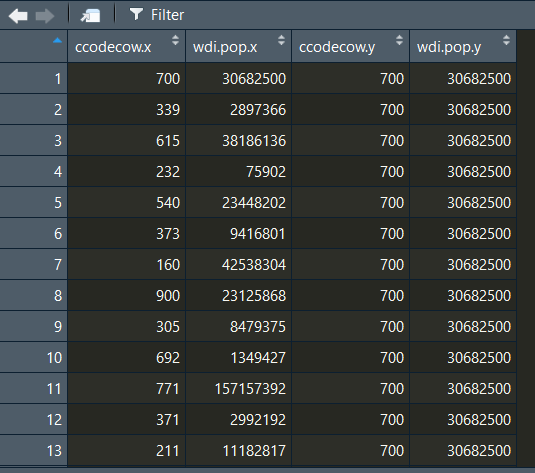
\includegraphics{r.post/merge.png}
\caption{이렇게 머지하면, x 국가군의 cowcode와 인구지표, 그리고 y 국가군의 cowcode를 가지게 됩니다.}
\end{figure}

이 경우에 동일한 국가쌍(self-dyads)은 제거해야 두 국가 간의 관계를 살펴볼 수 있을 것입니다. 동일한 국가의 인구 지표는 차이가 없으니까요!

\begin{Shaded}
\begin{Highlighting}[]
\KeywordTok{names}\NormalTok{(QOG.dyad)}
\end{Highlighting}
\end{Shaded}

\begin{verbatim}
## [1] "ccodecow.x" "wdi.pop.x"  "ccodecow.y" "wdi.pop.y"
\end{verbatim}

\begin{Shaded}
\begin{Highlighting}[]
\NormalTok{QOG.dyad <-}\StringTok{ }\KeywordTok{subset}\NormalTok{(QOG.dyad, ccodecow.x }\OperatorTok{!=}\StringTok{ }\NormalTok{ccodecow.y)}
\CommentTok{## QOG.dyad 자료에서 ccodecow.x가 ccodecow.y와 다른 경우만 다시 저장합니다.}
\NormalTok{QOG.dyad}\OperatorTok{$}\NormalTok{pop.dif <-}\StringTok{ }\NormalTok{QOG.dyad}\OperatorTok{$}\NormalTok{wdi.pop.x }\OperatorTok{-}\StringTok{ }\NormalTok{QOG.dyad}\OperatorTok{$}\NormalTok{wdi.pop.y}
\CommentTok{## QOG.dyad 데이터프레임에 pop.dif, 인구차이라는 변수를 새로 만듭니다.}
\CommentTok{## 인구 차이는 x국가의 wdi.pop.x에서 wdi.pop.y 를 감한 값입니다.}
\CommentTok{## 이 변수는 x국가와 y국가 간 인구 차이, 즉 두 국가 간의 역동적 관계를 보여줍니다.}
\end{Highlighting}
\end{Shaded}

위와 같이 \texttt{wdi.dif}라는 인구 차이 변수는 사실 \texttt{x}에서 \texttt{y}를 빼나 \texttt{y}에서 \texttt{x}를 빼나 부호를 제외하고 그 크기는 동일합니다. 따라서 우리는 따로 방향(direction)을 고려할 필요가 없습니다. 아래의 코드는 방향성을 제거한 국가쌍 자료(non-directed dyads)를 만드는 것입니다.

\begin{Shaded}
\begin{Highlighting}[]
\NormalTok{QOG.nddyad <-}\StringTok{ }\KeywordTok{subset}\NormalTok{(QOG.dyad, ccodecow.x }\OperatorTok{<}\StringTok{ }\NormalTok{ccodecow.y)}
\NormalTok{QOG.nddyad}\OperatorTok{$}\NormalTok{pop.dif.nd <-}\StringTok{ }\KeywordTok{abs}\NormalTok{(QOG.nddyad}\OperatorTok{$}\NormalTok{wdi.pop.x }\OperatorTok{-}\StringTok{ }\NormalTok{QOG.nddyad}\OperatorTok{$}\NormalTok{wdi.pop.y)}
\CommentTok{## abs는 absolute value, 부호를 고려하지 않기 위해서 절대값으로 만들라는 것입니다.}
\end{Highlighting}
\end{Shaded}

이번에는 국가-연도(country-year) 자료를 국가쌍-연도(dyad-year) 자료로 전환하는 사례를 살펴보겠습니다. 이를 위해서 일단 교차사례 시계열 데이터셋을 웹에서 다운받아 열어봅니다(time-series cross-sectional dataset). 이렇게 불러온 데이터셋은 1816년부터 2016년 사이의 국가들의 자료를 구축한 국가-연도를 분석단위로 한 자료입니다.

\begin{Shaded}
\begin{Highlighting}[]
\CommentTok{## COW 국가-연도 목록을 불러왔습니다.}
\NormalTok{stateyear <-}
\StringTok{  }\KeywordTok{read.csv}\NormalTok{(}\StringTok{"http://correlatesofwar.org/data-sets/state-system-membership/system2016"}\NormalTok{,}
                      \DataTypeTok{head =} \OtherTok{TRUE}\NormalTok{, }\DataTypeTok{sep =} \StringTok{","}\NormalTok{)}\CommentTok{# Look at country codes}
\KeywordTok{unique}\NormalTok{(stateyear}\OperatorTok{$}\NormalTok{ccode) }\CommentTok{# 중복되지 않는 국가코드만 보이게 했습니다.}
\end{Highlighting}
\end{Shaded}

\begin{verbatim}
##   [1]   2 200 210 220 225 230 235 245 255 267 269 271 273 275 300 325 327
##  [18] 329 337 365 380 390 640 140 616 350 211  70 100 240 135 155 101 160
##  [35] 332 280 150 600 145 335 130 630 651  41 710 740  90  92 345 360 165
##  [52] 730 800  42 530  91  93  40  95 385 355 339 375 290 310 315 366 367
##  [69] 368 305 700  20  94 212 450 560 790 900 920 712 205 678 670 645 395
##  [86] 652 660 663 840 750 770 666 731 775 780 713 732 850 620 811 812 265
## [103] 816 817 260 625 452 820 438 352 432 433 434 435 436 437 439 461 471
## [120] 475 481 482 483 484 490 520 580 451 510 690  51  52 500 516 517 615
## [137] 501 511 338 551 553 420 552 781 830  53 110 570 571 680 411 572 590
## [154] 950 692 694 696 698 760 771  31  55 404 115 402 403 540 541 581 910
## [171] 591 990 522  54 940  56  57  58  80 935  60 835 223 565 679 359 369
## [188] 370 371 372 373 701 702 703 704 705 983 987 331 344 346 349 221 232
## [205] 316 317 343 531 986 946 955 970 947 860 341 347 626
\end{verbatim}

\begin{Shaded}
\begin{Highlighting}[]
\KeywordTok{table}\NormalTok{(stateyear}\OperatorTok{$}\NormalTok{ccode)  }\CommentTok{# 각 국가코드가 몇 개의 관측치를 가지는지를 보여줍니다.}
\end{Highlighting}
\end{Shaded}

\begin{verbatim}
## 
##   2  20  31  40  41  42  51  52  53  54  55  56  57  58  60  70  80  90 
## 201  97  44 113 140 116  55  55  51  39  43  38  38  36  34 186  36 149 
##  91  92  93  94  95 100 101 110 115 130 135 140 145 150 155 160 165 200 
## 118 142 117  97 114 186 176  51  42 163 178 195 169 166 178 176 135 201 
## 205 210 211 212 220 221 223 225 230 232 235 240 245 255 260 265 267 269 
##  95 197 183  94 200  24  27 201 201  24 201  30  56 157  36  37  56  52 
## 271 273 275 280 290 300 305 310 315 316 317 325 327 329 331 332 335 337 
##  56  51  52  25  94 103  82  99  70  24  24 201  45  46  25  19  10  45 
## 338 339 341 343 344 345 346 347 349 350 352 355 359 360 365 366 367 368 
##  53  99  11  24  25 137  25   9  25 187  57 109  26 139 201  49  49  49 
## 369 370 371 372 373 375 380 385 390 395 402 403 404 411 420 432 433 434 
##  26  26  26  26  26 100 201 108 197  73  42  42  43  49  52  57  57  57 
## 435 436 437 438 439 450 451 452 461 471 475 481 482 483 484 490 500 501 
##  57  57  57  59  57  97  56  60  57  57  57  57  57  57  57  57  55  54 
## 510 511 516 517 520 522 530 531 540 541 551 552 553 560 565 570 571 572 
##  56   2  55  55  57  40 115  24  42  42  53  52  53  97  27  51  51  49 
## 580 581 590 591 600 615 616 620 625 626 630 640 645 651 652 660 663 666 
##  57  42  49  41 127  55 118  66  61   6 162 201  85 108  69  71  71  69 
## 670 678 679 680 690 692 694 696 698 700 701 702 703 704 705 710 712 713 
##  90  65  27  24  56  46  46  46  46  98  26  26  26  26  26 157  96  68 
## 730 731 732 740 750 760 770 771 775 780 781 790 800 811 812 816 817 820 
##  19  69  68 151  70  46  70  46  69  69  52  97 130  64  64  63  22  60 
## 830 835 840 850 860 900 910 920 935 940 946 947 950 955 970 983 986 987 
##  52  33  71  68  15  97  42  97  36  39  18  17  47  18  18  26  23  26 
## 990 
##  41
\end{verbatim}

불러온 목록에서 숫자형으로 저장된 \texttt{COW}국가 코드만 따로 떼어서 볼 수 있고, 코드별로 연도별 자료가 얼마나 관측되어 있는지 확인할 수 있습니다. 이제 여기서 연도와 \texttt{ccode} 변수만 따로 떼어보겠습니다.

\begin{Shaded}
\begin{Highlighting}[]
\NormalTok{stateyear <-}\StringTok{ }\KeywordTok{subset}\NormalTok{(stateyear, }\DataTypeTok{select =} \KeywordTok{c}\NormalTok{(year, ccode))}
\end{Highlighting}
\end{Shaded}

그리고 새로운 패키지, \texttt{countrycode()}를 이용하여 국가 이름 변수를 새롭게 만들어 데이터에 추가해보겠습니다.

\begin{Shaded}
\begin{Highlighting}[]
\CommentTok{## install.packages("countrycode")}
\KeywordTok{library}\NormalTok{(countrycode)}
\NormalTok{stateyear}\OperatorTok{$}\NormalTok{countryname <-}\StringTok{ }\KeywordTok{countrycode}\NormalTok{(stateyear}\OperatorTok{$}\NormalTok{ccode, }\StringTok{"cown"}\NormalTok{, }\StringTok{"country.name"}\NormalTok{)}
\CommentTok{## stateyear 자료에서 ccode 변수를 숫자형("cown")에서 문자형("country.name")으로 변경합니다.}
\CommentTok{## stateyear 자료에 countryname 이라는 새로운 이름 변수를 만들어 바꾼 자료를 배정합니다.}

\CommentTok{## 이 자료에서 결측치(missing values)를 제거해보겠습니다. }
\CommentTok{## complete.cases는 결측치를 제외한 변수들 짝이 완전하게 맞는 사례들만을 선별하라는 옵션입니다.}
\NormalTok{stateyear <-}\StringTok{ }\KeywordTok{subset}\NormalTok{(stateyear, }\KeywordTok{complete.cases}\NormalTok{(stateyear))}
\KeywordTok{head}\NormalTok{(stateyear)}
\end{Highlighting}
\end{Shaded}

\begin{verbatim}
##   year ccode    countryname
## 1 1816     2  United States
## 2 1816   200 United Kingdom
## 3 1816   210    Netherlands
## 4 1816   220         France
## 5 1816   225    Switzerland
## 6 1816   230          Spain
\end{verbatim}

연도 변수를 이용해서 이번에는 다시 국가쌍 자료로 머징해보겠습니다.

\begin{Shaded}
\begin{Highlighting}[]
\NormalTok{dyadyear <-}\StringTok{ }\KeywordTok{merge}\NormalTok{(}\DataTypeTok{x=}\NormalTok{stateyear, }\DataTypeTok{y=}\NormalTok{stateyear, }\DataTypeTok{by.x=}\KeywordTok{c}\NormalTok{(}\StringTok{"year"}\NormalTok{), }\DataTypeTok{by.y=}\KeywordTok{c}\NormalTok{(}\StringTok{"year"}\NormalTok{))}
\KeywordTok{head}\NormalTok{(dyadyear)}
\end{Highlighting}
\end{Shaded}

\begin{verbatim}
##   year ccode.x countryname.x ccode.y  countryname.y
## 1 1816       2 United States       2  United States
## 2 1816       2 United States     200 United Kingdom
## 3 1816       2 United States     210    Netherlands
## 4 1816       2 United States     220         France
## 5 1816       2 United States     225    Switzerland
## 6 1816       2 United States     230          Spain
\end{verbatim}

아까처럼 1행의 자기자신의 쌍을 구성하는 경우를 제거해보겠습니다. 이번에는 \texttt{subset()} 함수가 아니라 조건(condition, if)를 의미하는 대괄호를 이용해보겠습니다.

\begin{Shaded}
\begin{Highlighting}[]
\NormalTok{dyadyear <-}\StringTok{ }\NormalTok{dyadyear[dyadyear}\OperatorTok{$}\NormalTok{countryname.x }\OperatorTok{!=}\StringTok{ }\NormalTok{dyadyear}\OperatorTok{$}\NormalTok{countryname.y, ]}
\KeywordTok{head}\NormalTok{(dyadyear)}
\end{Highlighting}
\end{Shaded}

\begin{verbatim}
##   year ccode.x countryname.x ccode.y  countryname.y
## 2 1816       2 United States     200 United Kingdom
## 3 1816       2 United States     210    Netherlands
## 4 1816       2 United States     220         France
## 5 1816       2 United States     225    Switzerland
## 6 1816       2 United States     230          Spain
## 7 1816       2 United States     235       Portugal
\end{verbatim}

과연 이렇게 만든 게 자기쌍(self-dyads)을 잘 제거했는지 확인해볼 필요가 있습니다. 논리형 연산자(\texttt{==})를 이용하기 때문에 결과는 \texttt{TRUE} 또는 \texttt{FALSE}로 나타날 것입니다.

\begin{Shaded}
\begin{Highlighting}[]
\KeywordTok{table}\NormalTok{(dyadyear}\OperatorTok{$}\NormalTok{countryname.x }\OperatorTok{==}\StringTok{ }\NormalTok{dyadyear}\OperatorTok{$}\NormalTok{countryname.y)}
\end{Highlighting}
\end{Shaded}

\begin{verbatim}
## 
##   FALSE 
## 1881490
\end{verbatim}

이번에는 1980년 이후의 자료들만 가지고 국가쌍의 하위 데이터셋을 구해보겠습니다. 대괄호(\texttt{{[}{]}})와 \texttt{subset()} 함수를 이용한 방법 모두를 살펴보겠습니다.

\begin{Shaded}
\begin{Highlighting}[]
\CommentTok{## 대괄호 [] 를 이용한 방법}
\NormalTok{dyadyearp80 <-}\StringTok{ }\NormalTok{dyadyear[dyadyear}\OperatorTok{$}\NormalTok{year }\OperatorTok{>=}\StringTok{ }\DecValTok{1980}\NormalTok{,] }
\KeywordTok{glimpse}\NormalTok{(dyadyearp80)}
\end{Highlighting}
\end{Shaded}

\begin{verbatim}
## Observations: 1,205,276
## Variables: 5
## $ year          <int> 1980, 1980, 1980, 1980, 1980, 1980, 1980, 1980, ...
## $ ccode.x       <int> 2, 2, 2, 2, 2, 2, 2, 2, 2, 2, 2, 2, 2, 2, 2, 2, ...
## $ countryname.x <chr> "United States", "United States", "United States...
## $ ccode.y       <int> 20, 31, 40, 41, 42, 51, 52, 53, 54, 55, 56, 57, ...
## $ countryname.y <chr> "Canada", "Bahamas", "Cuba", "Haiti", "Dominican...
\end{verbatim}

\begin{Shaded}
\begin{Highlighting}[]
\CommentTok{## subset 함수를 이용한 방법}
\NormalTok{dyadyearp80 <-}\StringTok{ }\KeywordTok{subset}\NormalTok{(dyadyear, dyadyear}\OperatorTok{$}\NormalTok{year }\OperatorTok{>=}\StringTok{ }\DecValTok{1980}\NormalTok{)}
\KeywordTok{glimpse}\NormalTok{(dyadyearp80)}
\end{Highlighting}
\end{Shaded}

\begin{verbatim}
## Observations: 1,205,276
## Variables: 5
## $ year          <int> 1980, 1980, 1980, 1980, 1980, 1980, 1980, 1980, ...
## $ ccode.x       <int> 2, 2, 2, 2, 2, 2, 2, 2, 2, 2, 2, 2, 2, 2, 2, 2, ...
## $ countryname.x <chr> "United States", "United States", "United States...
## $ ccode.y       <int> 20, 31, 40, 41, 42, 51, 52, 53, 54, 55, 56, 57, ...
## $ countryname.y <chr> "Canada", "Bahamas", "Cuba", "Haiti", "Dominican...
\end{verbatim}

이번에는 변수들의 이름을 바꿔보겠습니다. 첫 번째는 기본 함수를 이용하고, 두 번째는 \texttt{plyr} 패키지를 이용해서 동일한 결과를 만들어 보겠습니다.

\begin{Shaded}
\begin{Highlighting}[]
\CommentTok{## 기본 함수를 이용해 변수명 바꾸기}
\CommentTok{## names(dyadyearp80)[변수 순서] <- "바꿀 변수 이름"}
\CommentTok{## 2번째 변수부터 5번째 변수들의 이름을 바꿔보자.}
\KeywordTok{names}\NormalTok{(dyadyearp80)[}\DecValTok{2}\OperatorTok{:}\DecValTok{5}\NormalTok{] <-}\StringTok{ }\KeywordTok{c}\NormalTok{(}\StringTok{"ccode1"}\NormalTok{, }\StringTok{"countryname1"}\NormalTok{, }
                             \StringTok{"ccode2"}\NormalTok{, }\StringTok{"countryname2"}\NormalTok{)}
\KeywordTok{head}\NormalTok{(dyadyearp80)}
\end{Highlighting}
\end{Shaded}

\begin{verbatim}
##        year ccode1  countryname1 ccode2       countryname2
## 685375 1980      2 United States     20             Canada
## 685376 1980      2 United States     31            Bahamas
## 685377 1980      2 United States     40               Cuba
## 685378 1980      2 United States     41              Haiti
## 685379 1980      2 United States     42 Dominican Republic
## 685380 1980      2 United States     51            Jamaica
\end{verbatim}

\begin{Shaded}
\begin{Highlighting}[]
\CommentTok{## install.packages("plyr")}
\KeywordTok{library}\NormalTok{(plyr)}
\NormalTok{dyadyearp80 <-}\StringTok{ }\KeywordTok{rename}\NormalTok{(dyadyearp80, }\KeywordTok{c}\NormalTok{(}\StringTok{"ccode.x"}\NormalTok{ =}\StringTok{ "ccode1"}\NormalTok{, }
                                     \StringTok{"ccode.y"}\NormalTok{ =}\StringTok{ "ccode2"}\NormalTok{,}
                                     \StringTok{"countryname.x"}\NormalTok{ =}\StringTok{ "countryname1"}\NormalTok{,}
                                     \StringTok{"countryname.y"}\NormalTok{ =}\StringTok{ "countryname2"}\NormalTok{))}
\end{Highlighting}
\end{Shaded}

\hypertarget{uxc608uxc81c-correlatesofwar.orguxc5d0uxc11c-capabilities-uxb370uxc774uxd130uxc14buxc744-uxbd88uxb7ecuxc624uxae303-3}{%
\subsection[예제: correlatesofwar.org에서 capabilities 데이터셋을 불러오기]{\texorpdfstring{예제: correlatesofwar.org에서 capabilities 데이터셋을 불러오기\footnote{단, 결측치를 의미하는 -9를 모두 NA로 바꿔서 불러 들여올 것입니다.}}{예제: correlatesofwar.org에서 capabilities 데이터셋을 불러오기}}\label{uxc608uxc81c-correlatesofwar.orguxc5d0uxc11c-capabilities-uxb370uxc774uxd130uxc14buxc744-uxbd88uxb7ecuxc624uxae303-3}}

\begin{Shaded}
\begin{Highlighting}[]
\NormalTok{cinc.link <-}\StringTok{ }
\StringTok{  "http://correlatesofwar.org/data-sets/national-material-capabilities/nmc-v4-data"}
\NormalTok{cinc <-}
\StringTok{  }\KeywordTok{read.csv}\NormalTok{(}\DataTypeTok{file =}\NormalTok{ cinc.link,}
           \DataTypeTok{head =} \OtherTok{TRUE}\NormalTok{,}
           \DataTypeTok{sep =} \StringTok{","}\NormalTok{,}
           \DataTypeTok{na =} \KeywordTok{c}\NormalTok{(}\OperatorTok{-}\DecValTok{9}\NormalTok{))}
\end{Highlighting}
\end{Shaded}

\texttt{COW} 홈페이지에서 \texttt{CINC} 데이터셋을 로드해보겠습니다. \texttt{CINC} (Composite Index of National Capability) Score는 국가-연도 별로 국가의 물질적 능력(national materials capabilities)에 대한 구성요소로서 측정된 여섯 가지 개별 지표들을 종합하여 한 지표로 만든 결과입니다 (Singer, Bremer and Stuckey, 1972).

\begin{itemize}
\tightlist
\item
  \texttt{CINC}는 각 구성요소를 동등하게 가중치를 부여하여 종합한 개별 연도마다의 능력 (capabilities)의 평균을 체계 전체 (total system)에서의 몫(share)으로 나타낸 것이다.
\item
  결과적으로 \texttt{CINC}는 0부터 1 사이의 값을 가지고 0은 해당 년도 체계 내에서 그 국가가 전체의 0\%의 능력을 가지고 있다는 것을 의미합니다.
\item
  반대로 1은 주어진 연도에서의 100\%의 역량을 보여줍니다 (Correlates of War Project National Material Capabilities (NMC) Data Documentation Version 5.0. Codebook 참조)
\end{itemize}

\texttt{CINC} 데이터셋을 \texttt{ID}와 \texttt{CINC\ score}의 두 변수만 갖도록 분할해보겠습니다.

\begin{Shaded}
\begin{Highlighting}[]
\NormalTok{cinc.cut <-}\StringTok{ }\NormalTok{cinc[}\KeywordTok{c}\NormalTok{(}\StringTok{"ccode"}\NormalTok{, }\StringTok{"year"}\NormalTok{, }\StringTok{"cinc"}\NormalTok{)]}
\end{Highlighting}
\end{Shaded}

\texttt{CINC} 값은 주어진 연도에서 국가쌍이 아닌, \textbf{한 국가}의 힘을 측정한 결과입니다. 그러나 우리는 이 \texttt{CINC} score를 이용해서 국가쌍의 변수로 만들 것이기 때문에, 먼저, 첫 번째 국가군 (country1 of \texttt{ccode1})에 대한 CINC 자료들을 머지해보겠습니다.

\begin{Shaded}
\begin{Highlighting}[]
\NormalTok{dyadcap <-}\StringTok{ }\KeywordTok{merge}\NormalTok{(}\DataTypeTok{x =}\NormalTok{ dyadyearp80,}
                 \DataTypeTok{y =}\NormalTok{ cinc.cut,}
                 \DataTypeTok{by.x =} \KeywordTok{c}\NormalTok{(}\StringTok{"ccode1"}\NormalTok{, }\StringTok{"year"}\NormalTok{),}
                 \DataTypeTok{by.y =} \KeywordTok{c}\NormalTok{(}\StringTok{"ccode"}\NormalTok{, }\StringTok{"year"}\NormalTok{))}
\NormalTok{dyadcap <-}\StringTok{ }\KeywordTok{rename}\NormalTok{(dyadcap, }\KeywordTok{c}\NormalTok{(}\StringTok{"cinc"}\NormalTok{ =}\StringTok{ "cinc1"}\NormalTok{))}
\KeywordTok{head}\NormalTok{(dyadcap)}
\end{Highlighting}
\end{Shaded}

\begin{verbatim}
##   ccode1 year countryname1 ccode2 countryname2     cinc1
## 1    100 1980     Colombia    572    Swaziland 0.0036558
## 2    100 1980     Colombia    581      Comoros 0.0036558
## 3    100 1980     Colombia    590    Mauritius 0.0036558
## 4    100 1980     Colombia    591   Seychelles 0.0036558
## 5    100 1980     Colombia    580   Madagascar 0.0036558
## 6    100 1980     Colombia    694        Qatar 0.0036558
\end{verbatim}

국가쌍의 역량을 보여주는 변수(dyad capabilities)라는 의미로 \texttt{dyadcap}이라는 데이터를 만들어았습니다. 머지할 첫 번째 데이터는 이전에 만들어 둔 \texttt{dyadyearp80}이고 두 번째 머지 대상 데이터는 \texttt{cinc.cut}입니다. \texttt{merge()} 함수는 나중에 따로 구체적으로 다루겠지만 아래의 \href{(https://www.rapidinsightinc.com/7-data-cleanup-terms-explained-visually/)}{그림}에서 개념을 개략적으로 파악할 수 있습니다.

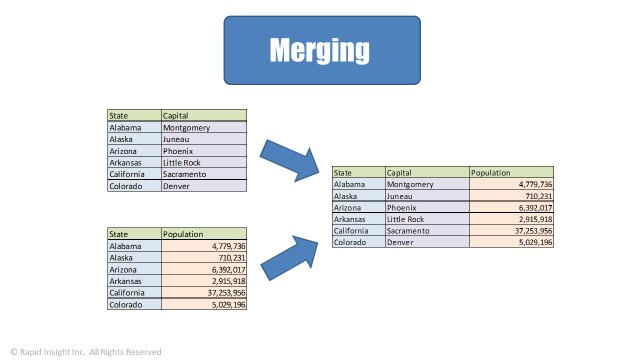
\includegraphics{r.post/Merging.jpg}

그림을 보면 \texttt{State} 변수를 기준으로 같은 \texttt{State}에 \texttt{Capital}과 \texttt{Population}이 묶인 것을 볼 수 있습니다다. 위의 R-code에서는 첫 번째 데이터에서는 \texttt{ccode1}과 \texttt{year} 변수를 기준으로, 두 번째 데이터에서는 \texttt{ccode}와 \texttt{year}를 기준으로 \texttt{dyadyearp80}의 \texttt{ccode1}과 \texttt{year}를 \texttt{cinc.cut}의 \texttt{ccode}와 \texttt{year}를 동일한 것으로 간주하여 두 변수를 하나의 데이터셋 안에 머지하라는 의미입니다.

국가쌍의 \texttt{CINC} 변수를 만든다는 것은 국가1과 국가2의 \texttt{CINC} 변수 두 개가 필요하다는 것입니다. 그렇다면 이후에 또 머지하여 추가될 변수와 기존의 변수가 충돌하지 않기 위해서 이름을 바꾸어줄 필요가 있습니다. 그래서 첫 번째 \texttt{CINC} 변수를 \texttt{CINC1}로 바꾸어주었습니다.

이제 국가2의 \texttt{CINC} score를 머지해보겠습니다. 앞서와의 동일한 과정을 진행하되 \texttt{ccode2}에 대한 \texttt{CINC} score를 머지해야 하니까 기준을 바꿔주면 됩니다.

\begin{Shaded}
\begin{Highlighting}[]
\NormalTok{dyadcap <-}\StringTok{ }\KeywordTok{merge}\NormalTok{(}\DataTypeTok{x =}\NormalTok{ dyadcap, }
                 \DataTypeTok{y =}\NormalTok{ cinc.cut, }
                 \DataTypeTok{by.x =} \KeywordTok{c}\NormalTok{(}\StringTok{"ccode2"}\NormalTok{, }\StringTok{"year"}\NormalTok{), }
                 \DataTypeTok{by.y =} \KeywordTok{c}\NormalTok{(}\StringTok{"ccode"}\NormalTok{, }\StringTok{"year"}\NormalTok{))}
\KeywordTok{head}\NormalTok{(dyadcap)}
\end{Highlighting}
\end{Shaded}

\begin{verbatim}
##   ccode2 year ccode1            countryname1 countryname2      cinc1
## 1    100 1980    541              Mozambique     Colombia 0.00097980
## 2    100 1980    680 Yemen People's Republic     Colombia 0.00035290
## 3    100 1980    490        Congo - Kinshasa     Colombia 0.00238030
## 4    100 1980    900               Australia     Colombia 0.00721210
## 5    100 1980     90               Guatemala     Colombia 0.00061660
## 6    100 1980    403     São Tomé & Príncipe     Colombia 0.00000384
##        cinc
## 1 0.0036558
## 2 0.0036558
## 3 0.0036558
## 4 0.0036558
## 5 0.0036558
## 6 0.0036558
\end{verbatim}

\begin{Shaded}
\begin{Highlighting}[]
\NormalTok{dyadcap <-}\StringTok{ }\KeywordTok{rename}\NormalTok{(dyadcap, }\KeywordTok{c}\NormalTok{(}\StringTok{"cinc"}\NormalTok{ =}\StringTok{ "cinc2"}\NormalTok{))}
\end{Highlighting}
\end{Shaded}

이렇게 만들어진 두 개의 \texttt{CINC} score를 이용하여 국가1과 국가2의 상대적 국력을 측정하는 변수를 새롭게 만들어 보겠습니다.

\begin{Shaded}
\begin{Highlighting}[]
\NormalTok{dyadcap}\OperatorTok{$}\NormalTok{caprat <-}\StringTok{ }\NormalTok{dyadcap}\OperatorTok{$}\NormalTok{cinc1}\OperatorTok{/}\NormalTok{dyadcap}\OperatorTok{$}\NormalTok{cinc2}
\end{Highlighting}
\end{Shaded}

이렇게 만들어진 변수는(데이터는) 방향성을 가진 국가쌍의 분석 수준의 자료입니다. 예를 들어, 이 자료에는 미국-캐나다 간의 국력과 캐나다-미국 간의 국력이 순서만 바뀐 채로 동일한 값 (동일한 \texttt{caprat} 변수값)을 가지고 있습니다.

이 중복된 값은 불필요하기 때문에 방향성을 제거할 필요가 있습니다(non-directed). 아래의 변수는 \texttt{ccode1}이 \texttt{ccode2}보다 작은 경우만을 남기라는 코드입니다. 즉, \texttt{ccode} 값이 2인 미국과 \texttt{ccode} 값이 731(맞나\ldots{}? 이거 쓸 때는 지금 코드북을 안보고 있숩\ldots{} 아마 우리나라 맞을 것인디\ldots{})인 한국의 상대적 국력 변수를 보면,

\begin{Shaded}
\begin{Highlighting}[]
\NormalTok{dyadcap }\OperatorTok\StringTok{ }\KeywordTok{select}\NormalTok{(ccode1, ccode2, year, caprat) }\OperatorTok
\StringTok{  }\NormalTok{dplyr}\OperatorTok{::}\KeywordTok{filter}\NormalTok{(ccode1 }\OperatorTok\StringTok{ }\KeywordTok{c}\NormalTok{(}\DecValTok{2}\NormalTok{, }\DecValTok{731}\NormalTok{), }
\NormalTok{                ccode2 }\OperatorTok\StringTok{ }\KeywordTok{c}\NormalTok{(}\DecValTok{2}\NormalTok{, }\DecValTok{731}\NormalTok{), }
\NormalTok{                year }\OperatorTok{==}\StringTok{ }\DecValTok{2000}\NormalTok{) }\OperatorTok\StringTok{ }
\StringTok{  }\NormalTok{knitr}\OperatorTok{::}\KeywordTok{kable}\NormalTok{()}
\end{Highlighting}
\end{Shaded}

\begin{tabular}{r|r|r|r}
\hline
ccode1 & ccode2 & year & caprat\\
\hline
731 & 2 & 2000 & 0.0712893\\
\hline
2 & 731 & 2000 & 14.0273479\\
\hline
\end{tabular}

로 두 국가 간의 국력비교 변수가 중복되어 있음을 확인할 수 있습니다. 이를

\begin{Shaded}
\begin{Highlighting}[]
\NormalTok{dyadcap }\OperatorTok\StringTok{ }
\StringTok{  }\NormalTok{dplyr}\OperatorTok{::}\KeywordTok{filter}\NormalTok{(ccode1 }\OperatorTok\StringTok{ }\DecValTok{2}\NormalTok{, }
\NormalTok{                ccode2 }\OperatorTok\StringTok{ }\DecValTok{731}\NormalTok{, }
\NormalTok{                year }\OperatorTok{==}\StringTok{ }\DecValTok{2000}\NormalTok{) }\OperatorTok\StringTok{ }\NormalTok{knitr}\OperatorTok{::}\KeywordTok{kable}\NormalTok{()}
\end{Highlighting}
\end{Shaded}

\begin{tabular}{r|r|r|l|l|r|r|r}
\hline
ccode2 & year & ccode1 & countryname1 & countryname2 & cinc1 & cinc2 & caprat\\
\hline
731 & 2000 & 2 & United States & North Korea & 0.1429513 & 0.0101909 & 14.02735\\
\hline
\end{tabular}

의 결과로 바꾸어주는 것입니다.

\begin{Shaded}
\begin{Highlighting}[]
\NormalTok{dyadcapnd <-}\StringTok{ }\NormalTok{dyadcap[dyadcap}\OperatorTok{$}\NormalTok{ccode1 }\OperatorTok{<}\StringTok{ }\NormalTok{dyadcap}\OperatorTok{$}\NormalTok{ccode2,]}
\end{Highlighting}
\end{Shaded}

이번에는 방향성을 제거한 국가쌍의 상대적 국력 지표를 만들어보겠습니다. 두 국가의 국력 중 큰 국력을 작은 국력으로 나누어서 상대적 국력 변수를 만들 것입니다.

\begin{Shaded}
\begin{Highlighting}[]
\NormalTok{dyadcapnd}\OperatorTok{$}\NormalTok{caprat <-}\StringTok{ }\KeywordTok{pmax}\NormalTok{(dyadcapnd}\OperatorTok{$}\NormalTok{cinc1, dyadcapnd}\OperatorTok{$}\NormalTok{cinc2)}\OperatorTok{/}
\StringTok{  }\KeywordTok{pmin}\NormalTok{(dyadcapnd}\OperatorTok{$}\NormalTok{cinc1, dyadcapnd}\OperatorTok{$}\NormalTok{cinc2)}
\KeywordTok{summary}\NormalTok{(dyadcapnd}\OperatorTok{$}\NormalTok{caprat)}
\end{Highlighting}
\end{Shaded}

\begin{verbatim}
##     Min.  1st Qu.   Median     Mean  3rd Qu.     Max. 
##      1.0      2.7      9.1    506.8     52.9 775694.9
\end{verbatim}

상대적 국력 변수라고 이름짓는 이유는 두 \texttt{cinc1}과 \texttt{cinc2}의 값이 같다면(상대적 국력이 같다면) 이 변수는 1의 값을 가질 것이고, 만약 \texttt{cinc1}이 \texttt{cinc2}에 비해 상대적으로 큰 국력을 가진다면 1보다 큰 값을 가질 것이기 때문입니다. 다만 \texttt{pmax()}와 \texttt{pmin()} 함수는 뒤에 포함된 괄호 안의 두 값 중 \texttt{최대값}과 \texttt{최소값}을 뽑아내라는 의미이므로 두 국가쌍의 값은 항상 최대값/최소값을 갖습니다.

만약 이 함수를 이용하지 않았더라면 \texttt{cinc1\ \textless{}\ cinc2} 인 상황에서 \texttt{cinc1/cinc2}로 계산되어, 1보다 작은 분수 값을 가지게 되었을 테지만, \texttt{pmax\ \&\ pmin} 조합을 통해서 우리는 1을 최소값으로 갖는 변수로 상대적 지표를 조작하게 된 것입니다.

\hypertarget{uxc694uxc57duxd1b5uxacc4uxd45cuxb97c-.tex-uxd30cuxc77cuxb85c-uxc800uxc7a5uxd558uxae30}{%
\section{요약통계표를 .tex 파일로 저장하기}\label{uxc694uxc57duxd1b5uxacc4uxd45cuxb97c-.tex-uxd30cuxc77cuxb85c-uxc800uxc7a5uxd558uxae30}}

\begin{Shaded}
\begin{Highlighting}[]
\KeywordTok{library}\NormalTok{(stargazer)}
\NormalTok{dyadcapnd <-}\StringTok{ }\KeywordTok{subset}\NormalTok{(dyadcapnd, }
                    \DataTypeTok{select =} \OperatorTok{-}\KeywordTok{c}\NormalTok{(countryname1, countryname2))}
\KeywordTok{glimpse}\NormalTok{(dyadcapnd)}
\end{Highlighting}
\end{Shaded}

\begin{verbatim}
## Observations: 434,728
## Variables: 6
## $ ccode2 <int> 100, 100, 100, 100, 100, 100, 100, 100, 100, 100, 100, ...
## $ year   <int> 1980, 1980, 1980, 1980, 1980, 1980, 1980, 1980, 1980, 1...
## $ ccode1 <int> 90, 70, 94, 55, 92, 54, 53, 31, 56, 20, 2, 40, 93, 95, ...
## $ cinc1  <dbl> 0.00061660, 0.01232570, 0.00020330, 0.00001250, 0.00048...
## $ cinc2  <dbl> 0.0036558, 0.0036558, 0.0036558, 0.0036558, 0.0036558, ...
## $ caprat <dbl> 5.928965, 3.371547, 17.982292, 292.464000, 7.545511, 10...
\end{verbatim}

\texttt{=\ -c} 표시는 이 기호 뒤의 벡터를 제외한 모든 변수들을 선택하여 하위 데이터셋을 만들라는 명령입니다. 혹은 아래와 같이 포함하고 싶은 변수들을 벡터로 하나하나 다 적어도 됩니다.
\texttt{stargazer()} 함수를 이용해서 요약통계치를 만들 때에는 굳이 국가명이 필요하진 않으니 제외하였습니다.

\begin{Shaded}
\begin{Highlighting}[]
\NormalTok{stat.table <-}\StringTok{ }\KeywordTok{stargazer}\NormalTok{(dyadcapnd, }
                        \DataTypeTok{covariate.labels =} 
                          \KeywordTok{c}\NormalTok{(}\StringTok{"Country code 1"}\NormalTok{, }
                            \StringTok{"Country code 2"}\NormalTok{, }\StringTok{"Year"}\NormalTok{, }
                            \StringTok{"CINC 1"}\NormalTok{, }\StringTok{"CINC 2"}\NormalTok{, }
                            \StringTok{"Capability ratio"}\NormalTok{), }
                        \DataTypeTok{title =} \StringTok{"Summary Statistics"}\NormalTok{,}
                        \DataTypeTok{label =} \StringTok{"stat.table"}\NormalTok{)}
\KeywordTok{write}\NormalTok{(}\DataTypeTok{x =}\NormalTok{ stat.table, }\DataTypeTok{file =} \StringTok{"tables/table1.tex"}\NormalTok{)}
\end{Highlighting}
\end{Shaded}

.tex 파일에 대한 소개는 다른 탭의 포스팅을 통해 진행하도록 하겠습니다. 일단 여기서는 코드만 알아두고 써먹을 일 있으면 \texttt{copy\ \&\ paste} 해보시기 바랍니다.

\hypertarget{uxc11cuxb85c-uxb2e4uxb978-uxbd84uxc11duxc218uxc900lower-higher-uxd1b5uxd569uxd558uxae30}{%
\section{서로 다른 분석수준(lower \& higher) 통합하기}\label{uxc11cuxb85c-uxb2e4uxb978-uxbd84uxc11duxc218uxc900lower-higher-uxd1b5uxd569uxd558uxae30}}

일단 \texttt{COW}의 양자간 무역 데이터(Correlates of War trade bilateral data version 3.0)를 불러오겠습니다자. 이 변수는 csv 또는 dta 파일과는 달리 \href{http://www.correlatesofwar.org/COW2\%20Data/Trade/Trade.html}{온라인}에 게재되어 있기 때문에 바로 객체로 불러와 열 수는 없습니다. 따라서 먼저 압축파일(zip)의 형식으로 다운받고 난 뒤에 그 압축파일에서 필요한 자료를 추출해내야 합니다.

\begin{Shaded}
\begin{Highlighting}[]
\NormalTok{link <-}\StringTok{ "http://correlatesofwar.org/data-sets/bilateral-trade/cow_trade_3.0"}
\KeywordTok{download.file}\NormalTok{(}\DataTypeTok{url =}\NormalTok{ link,}
              \DataTypeTok{destfile =} \StringTok{"COWTrade3.0.zip"}\NormalTok{, }\DataTypeTok{mode=}\StringTok{"wb"}\NormalTok{)}
\KeywordTok{unzip}\NormalTok{(}\StringTok{"COWTrade3.0.zip"}\NormalTok{, }\DataTypeTok{exdir =} \KeywordTok{getwd}\NormalTok{())}
\end{Highlighting}
\end{Shaded}

압축을 푼 파일을 \textbf{R}의 객체로 불러들여 열고 분석할 것입니다. 데이터는 압축이 풀린 폴더의 하위에 있기 때문에 그 디렉토리를 정확하게 반영하여 코드를 짜야 합니다.\footnote{정말 짜증나는군요. 이런 데이터는 써주지 말아야 합니다. \texttt{COW} 불매운동\ldots{}}

\begin{Shaded}
\begin{Highlighting}[]
\NormalTok{btrade <-}\StringTok{ }\KeywordTok{read.csv}\NormalTok{(}\DataTypeTok{file =} \StringTok{"COW_Trade_3.0/dyadic_trade_3.0.csv"}\NormalTok{)}
\KeywordTok{names}\NormalTok{(btrade)}
\end{Highlighting}
\end{Shaded}

\begin{verbatim}
##  [1] "ccode1"            "ccode2"            "year"             
##  [4] "importer1"         "importer2"         "flow1"            
##  [7] "flow2"             "source1"           "source2"          
## [10] "bel_lux_alt_flow1" "bel_lux_alt_flow2" "china_alt_flow1"  
## [13] "china_alt_flow2"   "version"
\end{verbatim}

\begin{Shaded}
\begin{Highlighting}[]
\KeywordTok{glimpse}\NormalTok{(btrade)}
\end{Highlighting}
\end{Shaded}

\begin{verbatim}
## Observations: 791,490
## Variables: 14
## $ ccode1            <dbl> 2, 2, 2, 2, 2, 2, 2, 2, 2, 2, 2, 2, 2, 2, 2,...
## $ ccode2            <int> 20, 20, 20, 20, 20, 20, 20, 20, 20, 20, 20, ...
## $ year              <int> 1920, 1921, 1922, 1923, 1924, 1925, 1926, 19...
## $ importer1         <fct> United States of America, United States of A...
## $ importer2         <fct> Canada, Canada, Canada, Canada, Canada, Cana...
## $ flow1             <dbl> 611.86, 335.44, 364.02, 416.00, 399.14, 473....
## $ flow2             <dbl> 735.48, 442.99, 502.84, 598.14, 496.32, 608....
## $ source1           <int> 1, 1, 1, 1, 1, 1, 1, 1, 1, 1, -9, 1, 1, 1, 1...
## $ source2           <int> 1, 1, 1, 1, 1, 1, 1, 1, 1, 1, 1, 1, 1, 1, 1,...
## $ bel_lux_alt_flow1 <dbl> -9, -9, -9, -9, -9, -9, -9, -9, -9, -9, -9, ...
## $ bel_lux_alt_flow2 <dbl> -9, -9, -9, -9, -9, -9, -9, -9, -9, -9, -9, ...
## $ china_alt_flow1   <dbl> -9, -9, -9, -9, -9, -9, -9, -9, -9, -9, -9, ...
## $ china_alt_flow2   <dbl> -9, -9, -9, -9, -9, -9, -9, -9, -9, -9, -9, ...
## $ version           <dbl> 2.01, 2.01, 2.01, 2.01, 2.01, 2.01, 2.01, 2....
\end{verbatim}

이렇게 불러들여온 양자간 무역 자료의 분석수준은 무엇일까요? 그리고 각 변수들은 무엇을 의미할까요? 이러한 내용은 \textbf{R}로 불러들여온 자료만으로는 알 수 없습니다. 따라서 항상 데이터셋을 다운받을 때는 코드북을 같이 다운 받아서 숙지하는 습관을 들일 필요가 있습니다. 일단 당장의 분석에 필요없는 변수들을 날려버리겠습니다.

\begin{Shaded}
\begin{Highlighting}[]
\NormalTok{btrade}\OperatorTok{$}\NormalTok{source2 <-}\StringTok{ }
\StringTok{  }\NormalTok{btrade}\OperatorTok{$}\NormalTok{bel_lux_alt_flow1 <-}\StringTok{ }
\StringTok{  }\NormalTok{btrade}\OperatorTok{$}\NormalTok{bel_lux_alt_flow2 <-}\StringTok{ }
\StringTok{  }\NormalTok{btrade}\OperatorTok{$}\NormalTok{china_alt_flow1 <-}\StringTok{ }
\StringTok{  }\NormalTok{btrade}\OperatorTok{$}\NormalTok{china_alt_flow2 <-}\StringTok{ }
\StringTok{  }\NormalTok{btrade}\OperatorTok{$}\NormalTok{version <-}\StringTok{ }\OtherTok{NULL}
\KeywordTok{glimpse}\NormalTok{(btrade)}
\end{Highlighting}
\end{Shaded}

\begin{verbatim}
## Observations: 791,490
## Variables: 8
## $ ccode1    <dbl> 2, 2, 2, 2, 2, 2, 2, 2, 2, 2, 2, 2, 2, 2, 2, 2, 2, 2...
## $ ccode2    <int> 20, 20, 20, 20, 20, 20, 20, 20, 20, 20, 20, 20, 20, ...
## $ year      <int> 1920, 1921, 1922, 1923, 1924, 1925, 1926, 1927, 1928...
## $ importer1 <fct> United States of America, United States of America, ...
## $ importer2 <fct> Canada, Canada, Canada, Canada, Canada, Canada, Cana...
## $ flow1     <dbl> 611.86, 335.44, 364.02, 416.00, 399.14, 473.72, 974....
## $ flow2     <dbl> 735.48, 442.99, 502.84, 598.14, 496.32, 608.35, 609....
## $ source1   <int> 1, 1, 1, 1, 1, 1, 1, 1, 1, 1, -9, 1, 1, 1, 1, 1, 1, ...
\end{verbatim}

중요한 것은 이 데이터셋에서 결측치는 \texttt{NA}가 아니라 \texttt{-9}로 코딩되어 있다는 사실입니다. 만약 이 \texttt{-9}들을 가만히 놔뒀다가는 요약통계와 추론통계를 부정확하게 만들 것이기 때문에 \texttt{flow1}과 \texttt{flow2}의 결측치들을 \texttt{NA}로 바꾸어 주어야 합니다. 사실 csv 파일을 불러들여올 때 했을 수도 있지만 여기서는 불러들인 상황에서 뒤늦게 \texttt{-9}를 발견하고 바꾸는 대처 방법을 배워봅시다.

\begin{Shaded}
\begin{Highlighting}[]
\NormalTok{btrade}\OperatorTok{$}\NormalTok{flow1[btrade}\OperatorTok{$}\NormalTok{flow1 }\OperatorTok{==}\StringTok{ }\DecValTok{-9}\NormalTok{] <-}\StringTok{ }\OtherTok{NA} \CommentTok{# 대괄호는 조건(condition)을 의미합니다.}
\NormalTok{btrade}\OperatorTok{$}\NormalTok{flow2[btrade}\OperatorTok{$}\NormalTok{flow2 }\OperatorTok{==}\StringTok{ }\DecValTok{-9}\NormalTok{] <-}\StringTok{ }\OtherTok{NA}
\KeywordTok{summary}\NormalTok{(btrade}\OperatorTok{$}\NormalTok{flow1) }\CommentTok{# -9이 사라졌습니다.}
\end{Highlighting}
\end{Shaded}

\begin{verbatim}
##     Min.  1st Qu.   Median     Mean  3rd Qu.     Max.     NA's 
##      0.0      0.0      0.1    158.4      6.0 363989.6   224291
\end{verbatim}

개별 국가들의 연간 총무역량을 계산해보겠습니다. 먼저 국가쌍의 수입(imports)과 수출(exports)을 더합니다. 이때 만약 \texttt{flow1}나 \texttt{flow2} 둘 중 하나가 결측치일 경우 총무역량 또한 결측치로 나타날 것입니다. 따라서 단순 더하기 코드로는 결과가 왜곡될 수 있습니다.

\begin{Shaded}
\begin{Highlighting}[]
\NormalTok{btrade}\OperatorTok{$}\NormalTok{tottrade1 <-}\StringTok{ }\NormalTok{btrade}\OperatorTok{$}\NormalTok{flow1 }\OperatorTok{+}\StringTok{ }\NormalTok{btrade}\OperatorTok{$}\NormalTok{flow2 }\CommentTok{# 잘못된 결과를 얻게 됩니다.}
\KeywordTok{summary}\NormalTok{(btrade}\OperatorTok{$}\NormalTok{tottrade1)}
\end{Highlighting}
\end{Shaded}

\begin{verbatim}
##      Min.   1st Qu.    Median      Mean   3rd Qu.      Max.      NA's 
##       0.0       0.0       1.0     315.1      18.9 1198528.8    250983
\end{verbatim}

\begin{Shaded}
\begin{Highlighting}[]
\NormalTok{btrade}\OperatorTok{$}\NormalTok{tottrade2 <-}\StringTok{ }\KeywordTok{ifelse}\NormalTok{(}\KeywordTok{is.na}\NormalTok{(btrade}\OperatorTok{$}\NormalTok{flow1), btrade}\OperatorTok{$}\NormalTok{flow2,}
                          \KeywordTok{ifelse}\NormalTok{(}\KeywordTok{is.na}\NormalTok{(btrade}\OperatorTok{$}\NormalTok{flow2), btrade}\OperatorTok{$}\NormalTok{flow1,}
\NormalTok{                                 btrade}\OperatorTok{$}\NormalTok{flow1 }\OperatorTok{+}\StringTok{ }\NormalTok{btrade}\OperatorTok{$}\NormalTok{flow2))}
\KeywordTok{summary}\NormalTok{(btrade}\OperatorTok{$}\NormalTok{tottrade2)}
\end{Highlighting}
\end{Shaded}

\begin{verbatim}
##      Min.   1st Qu.    Median      Mean   3rd Qu.      Max.      NA's 
##       0.0       0.0       0.6     289.0      14.6 1198528.8    202128
\end{verbatim}

첫 번째 코드는 \texttt{flow1}과 \texttt{flow2} (수입과 수출)을 더하여 \texttt{총무역량1}이라는 변수를 만들라는 것입니다. 이때, 둘 중 하나에 결측치가 있으면 그 합 역시 결측치가 됩니다.

이 문제를 피하기 위한 두 번째 코드는 만약 \texttt{flow1}이 결측치라면 \texttt{총무역량2}라는 변수에 \texttt{flow2}의 값을 부여하라는 얘기이고 만약 \texttt{flow1}이 결측치가 아니며, 동시에 \texttt{flow2}는 결측치라면 그 자리에 \texttt{flow1} 값을 부여하라는 얘기입니다. 만약 둘 다 결측치가 아닐 경우에는 마지막의 조건, \texttt{flow1}과 \texttt{flow2}를 결합한 값을 넣으라는 얘기입니다.

이와 같은 결과는 \texttt{plyr} 패키지를 이용해서도 얻을 수 있습니다. \texttt{plyr}패키지의 \texttt{summarise()} 함수를 이용하여 새로운 데이터프레임을 만들 수 있습니다. 물론 기존 데이터프레임으로 지정하면 새롭게 통합(aggregate)된 자료로 대체됩니다.

이렇게 얻은 \texttt{styrtrade1}이라는 변수는 \texttt{ccode1}과 \texttt{year} 단위로 결측치를 제외하고(\texttt{na.rm\ =\ TRUE}) 총무역값을 전부 더한 결과입니다. 그리고 그 양자간 무역 총액 변수를 머지하여 \texttt{btrade} 데이터에 붙여줍니다. 이제 \texttt{국가1}의 \texttt{특정연도} 하에서의 양자간 무역과 그 해의 총액을 확인할 수 있습니다.

아래의 코드로 만든 \texttt{share1}은 \texttt{국가1(state1)}의 총무역량에서 양자간 무역이 차지하는 비율을 보여줍니다.

\begin{Shaded}
\begin{Highlighting}[]
\KeywordTok{library}\NormalTok{(plyr)}
\NormalTok{btrade <-}\StringTok{ }\KeywordTok{ddply}\NormalTok{(btrade, .(ccode1, year), }
\NormalTok{                transform, }\DataTypeTok{styrtrade1 =} \KeywordTok{sum}\NormalTok{(tottrade2, }\DataTypeTok{na.rm =} \OtherTok{TRUE}\NormalTok{))}
\NormalTok{btrade}\OperatorTok{$}\NormalTok{share1 <-}\StringTok{ }\NormalTok{btrade}\OperatorTok{$}\NormalTok{tottrade2 }\OperatorTok{/}\StringTok{ }\NormalTok{btrade}\OperatorTok{$}\NormalTok{styrtrade1 }
\end{Highlighting}
\end{Shaded}

오늘의 포스팅에서는 꽤나 여러 가지 자료들을 다루어 보았는데, 좀 복잡할 수도 있습니다. 사실 저도 IR 쪽 자료는 잘 사용하지 않고 교차사례 시계열로만 쓰는데 IR은 그걸 국가쌍의 자료로(dyadic) 재구성해서 국가들 간의 관계를 살펴보는 연구들도 합니다. 여하튼 이번 포스팅에서는 \texttt{plyr}패키지의 사용을 확인하고 숙지하는 것만 건져도 승리하는 것이라고 할 수 있겠습니다.

\hypertarget{probability-into-r}{%
\chapter{Probability into R}\label{probability-into-r}}

확률 관련 포스팅에서는 몇 가지 간단한 확률을 \textbf{R}을 통해서 증명하고(Some simple probability demonstrations), 정규분포(normal distributions)와 이항분포(binomial distributions)로부터 분위(quantiles)를 얻어내는 방법을 살펴보고자 합니다.

여기서는 일단 간단하게 정규분포랑 이항분포, 그리고 독립사건과 종속사건만 간단하게 살펴보겠습니다.

\begin{itemize}
\tightlist
\item
  분위(Quantiles)에 대해 어떻게 설명할까 고민을 좀 했는데 좋은 블로그 포스팅을 찾아서 참조용으로 링크하겠습니다.
\item
  링크는 \href{https://blog.naver.com/sw4r/221026102874}{여기}를 보시면 됩니다. Q-Q Plot 설명하면서 Quantile의 정의도 잘 정리해놓으셨습니다.
\end{itemize}

그럼 본격적으로 포스팅을 시작하기에 앞서서 항상 그렇듯이 작업 디렉토리를 설정해보겠습니다.

\begin{Shaded}
\begin{Highlighting}[]
\KeywordTok{rm}\NormalTok{(}\DataTypeTok{list=}\KeywordTok{ls}\NormalTok{()) }\CommentTok{# 현재 콘솔 창에 저장되어 있는 모든 값과 모델 등을 삭제 }
\end{Highlighting}
\end{Shaded}

\begin{Shaded}
\begin{Highlighting}[]
\KeywordTok{library}\NormalTok{(here)}
\KeywordTok{library}\NormalTok{(knitr)}
\KeywordTok{library}\NormalTok{(dplyr)}
\KeywordTok{library}\NormalTok{(tidyverse)}
\KeywordTok{library}\NormalTok{(kableExtra)}
\NormalTok{here}\OperatorTok{::}\KeywordTok{here}\NormalTok{() }\OperatorTok\StringTok{ }\KeywordTok{setwd}\NormalTok{()}
\end{Highlighting}
\end{Shaded}

\hypertarget{uxc8fcuxc0acuxc704uxad74uxb9acuxae30-uxac8cuxc784}{%
\section{주사위굴리기 게임!}\label{uxc8fcuxc0acuxc704uxad74uxb9acuxae30-uxac8cuxc784}}

확률을 공부할 때, 지겹도록 등장하는 놈들이 총 셋이 있습니다. 동전, 카드, 그리고 주사위입니다. 인류는 아마도 이 셋을 만듦으로써 스스로를 괴롭히는 통계학을 발전시켰는지도 모르겠습니다\ldots{} 일단 주사위 굴리기는 직관적으로 확률과 통계를 이해하기 좋은 방식입니다. 먼저 주사위 하나를 한 번 굴리는 것을 시뮬레이팅하는 함수를 코딩해보겠습니다.

\begin{Shaded}
\begin{Highlighting}[]
\NormalTok{die <-}\StringTok{ }\KeywordTok{as.integer}\NormalTok{(}\KeywordTok{runif}\NormalTok{(}\DecValTok{1}\NormalTok{, }\DataTypeTok{min=}\DecValTok{1}\NormalTok{, }\DataTypeTok{max=}\DecValTok{7}\NormalTok{))}
\NormalTok{die}
\end{Highlighting}
\end{Shaded}

\begin{verbatim}
## [1] 5
\end{verbatim}

\texttt{die}는 \texttt{?runif} 라고 입력하여 살펴보면 \texttt{generates\ random\ deviates.}라고 기술되어 있는 것을 확인할 수 있습니다. 이어지는 함수를 풀어서 설명하면 다음과 같습니다.: 다음의 결과를 정수의 형태로 저장하라(\texttt{as.integer}) \(\rightarrow\) 무작위로 다음의 범주 내에서 다른 값을 1번 추출하라 \(\rightarrow\) 최소값은 1, 최대값은 6 (1 이상 7미만)을 갖게하라.

그러면 이번에는 두 개의 주사위를 굴려보도록 하겠습니다. 굴리는 횟수는 한 번입니다.

\begin{Shaded}
\begin{Highlighting}[]
\NormalTok{dice <-}\StringTok{ }\NormalTok{(}\KeywordTok{as.integer}\NormalTok{(}\KeywordTok{runif}\NormalTok{(}\DecValTok{1}\NormalTok{, }\DataTypeTok{min=}\DecValTok{1}\NormalTok{, }\DataTypeTok{max=}\DecValTok{7}\NormalTok{))) }\OperatorTok{+}
\StringTok{  }\NormalTok{(}\KeywordTok{as.integer}\NormalTok{(}\KeywordTok{runif}\NormalTok{(}\DecValTok{1}\NormalTok{, }\DataTypeTok{min=}\DecValTok{1}\NormalTok{, }\DataTypeTok{max=}\DecValTok{7}\NormalTok{)))}
\NormalTok{dice}
\end{Highlighting}
\end{Shaded}

\begin{verbatim}
## [1] 8
\end{verbatim}

여기서 \texttt{+} 연산자는 부울리안 논리에 따르면 \texttt{OR}를 의미합니다. 즉 각 주사위를 한 번씩 랜덤으로 굴려 얻는 값을 더한 결과를 \texttt{dice}에 저장하라는 명령입니다. 그럼 이번에는 100번, 1000번, 그리고 100만번을 돌려겠습니다.

\begin{Shaded}
\begin{Highlighting}[]
\CommentTok{# 주사위 두 개를 100번 던져보기}
\NormalTok{dice100 <-}\StringTok{  }\NormalTok{(}\KeywordTok{as.integer}\NormalTok{(}\KeywordTok{runif}\NormalTok{(}\DecValTok{100}\NormalTok{, }\DataTypeTok{min=}\DecValTok{1}\NormalTok{, }\DataTypeTok{max=}\DecValTok{7}\NormalTok{))) }\OperatorTok{+}
\StringTok{  }\NormalTok{(}\KeywordTok{as.integer}\NormalTok{(}\KeywordTok{runif}\NormalTok{(}\DecValTok{100}\NormalTok{, }\DataTypeTok{min=}\DecValTok{1}\NormalTok{, }\DataTypeTok{max=}\DecValTok{7}\NormalTok{)))}

\CommentTok{# 주사위 두 개를 1,000번 던져보기}
\NormalTok{dice1000 <-}\StringTok{  }\NormalTok{(}\KeywordTok{as.integer}\NormalTok{(}\KeywordTok{runif}\NormalTok{(}\DecValTok{1000}\NormalTok{, }\DataTypeTok{min=}\DecValTok{1}\NormalTok{, }\DataTypeTok{max=}\DecValTok{7}\NormalTok{))) }\OperatorTok{+}
\StringTok{  }\NormalTok{(}\KeywordTok{as.integer}\NormalTok{(}\KeywordTok{runif}\NormalTok{(}\DecValTok{1000}\NormalTok{, }\DataTypeTok{min=}\DecValTok{1}\NormalTok{, }\DataTypeTok{max=}\DecValTok{7}\NormalTok{)))}

\CommentTok{# 주사위 두 개를 100만 번 던져보기}
\NormalTok{dice1M <-}\StringTok{  }\NormalTok{(}\KeywordTok{as.integer}\NormalTok{(}\KeywordTok{runif}\NormalTok{(}\DecValTok{1000000}\NormalTok{, }\DataTypeTok{min=}\DecValTok{1}\NormalTok{, }\DataTypeTok{max=}\DecValTok{7}\NormalTok{))) }\OperatorTok{+}\StringTok{ }
\StringTok{  }\NormalTok{(}\KeywordTok{as.integer}\NormalTok{(}\KeywordTok{runif}\NormalTok{(}\DecValTok{1000000}\NormalTok{, }\DataTypeTok{min=}\DecValTok{1}\NormalTok{, }\DataTypeTok{max=}\DecValTok{7}\NormalTok{)))}
\end{Highlighting}
\end{Shaded}

이렇게 시뮬레이팅한 세 결과를 히스토그램으로 살펴보겠습니다.

\begin{Shaded}
\begin{Highlighting}[]
\KeywordTok{par}\NormalTok{(}\DataTypeTok{mfrow =} \KeywordTok{c}\NormalTok{(}\DecValTok{1}\NormalTok{, }\DecValTok{3}\NormalTok{))}
\KeywordTok{hist}\NormalTok{(dice1000)}
\KeywordTok{hist}\NormalTok{(dice100)}
\KeywordTok{hist}\NormalTok{(dice1M)}
\end{Highlighting}
\end{Shaded}

\begin{center}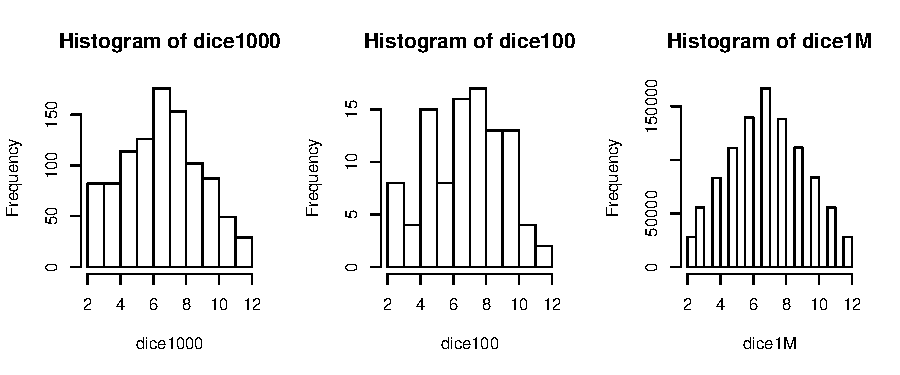
\includegraphics{Kor_BasicStats_files/figure-latex/unnamed-chunk-83-1} \end{center}

일단 가시적으로 살펴볼 수 있게 각 코드 이후에 그 결과값의 빈도를 표로 나타내보았습니다. 그리고 그 표를 히스토그램으로 재구성해보았습니다. 역시 \texttt{N}이 늘어날 수록 우리(?)가 사랑하는 그 녀석의 모습이 드러나기 시작합니다.

주사위는 1에서 6까지의 한정된 값을 가지고, 두 개를 합쳐서 굴려봐야 2부터 12까지의 한정된(bounded) 값이긴 하지만 이 주사위 굴리기를 통해서 우리는 지난 번 포스팅에서 살펴보았던 것처럼 정규분포(normal distribution)와 표본 크기(n), 혹은 표집(sampling)의 관계를 간접적으로 다시 한 번 살펴볼 수 있습니다.

\hypertarget{uxb3d9uxc804-uxb358uxc9c0uxae30}{%
\section{동전 던지기}\label{uxb3d9uxc804-uxb358uxc9c0uxae30}}

그럼 이번에는 동전을 한 번 던져보겠습니다. 저는 아직까지 앞면 뒷면 이외에 옆면에도 표기를 지닌 동전을 본 적이 없으니, 여기서의 동전도 앞면과 뒷면이라는 두 개의 값만을 가진다고 가정하겠습니다. 삼면이나 사면을 가진 동전을 보신 분들은 부디 댓글로 알려주시길\ldots{} 나와라 검은 백조야(김웅진 · 김지희 2012, p.53).

아무튼 앞면과 뒷면이 있는 경우에 그 각각이 나올 확률은 0.5, 0.5라고 할 수 있습니다. \texttt{rbinom()}은, randomly {[}drawn{]} binomial, 무작위로 이항변수를 추출하라는 함수라고 할 수 있습니다. 백문이 불여일코드.

\begin{Shaded}
\begin{Highlighting}[]
\NormalTok{coin <-}\StringTok{ }\KeywordTok{rbinom}\NormalTok{(}\DecValTok{1}\NormalTok{, }\DecValTok{1}\NormalTok{, }\FloatTok{.5}\NormalTok{)}
\NormalTok{coin}
\end{Highlighting}
\end{Shaded}

\begin{verbatim}
## [1] 1
\end{verbatim}

이어지는 함수를 풀어서 설명하면 다음과 같습니다.: 이항변수로 무작위로 추출하라(\texttt{rbinom()}) \(\rightarrow\) 1번 추출하라 \(\rightarrow\) 최대값은 1 (=최소값은 0) \(\rightarrow\) 추출확률은 0.5. 즉, 1이 나올 확률을 50\%로 설정하여 무작위로 추출하라는 것입니다. 그럼 이번에는 100개의 동전을 던져보겠습니다.

\begin{Shaded}
\begin{Highlighting}[]
\CommentTok{# 동전 100개 던지기}
\NormalTok{coin100 <-}\StringTok{ }\KeywordTok{rbinom}\NormalTok{(}\DecValTok{100}\NormalTok{, }\DecValTok{1}\NormalTok{, }\FloatTok{.5}\NormalTok{)}
\NormalTok{coin100 }\OperatorTok\StringTok{ }\KeywordTok{table}\NormalTok{() }\OperatorTok\StringTok{ }\KeywordTok{kable}\NormalTok{()}
\end{Highlighting}
\end{Shaded}

\begin{tabular}{l|r}
\hline
. & Freq\\
\hline
0 & 56\\
\hline
1 & 44\\
\hline
\end{tabular}

\begin{Shaded}
\begin{Highlighting}[]
\CommentTok{#동전 1000개 던지기}
\NormalTok{coin1000 <-}\StringTok{ }\KeywordTok{rbinom}\NormalTok{(}\DecValTok{1000}\NormalTok{, }\DecValTok{1}\NormalTok{, }\FloatTok{.5}\NormalTok{)}
\NormalTok{coin1000 }\OperatorTok\StringTok{ }\KeywordTok{table}\NormalTok{() }\OperatorTok\StringTok{ }\KeywordTok{kable}\NormalTok{()}
\end{Highlighting}
\end{Shaded}

\begin{tabular}{l|r}
\hline
. & Freq\\
\hline
0 & 490\\
\hline
1 & 510\\
\hline
\end{tabular}

\begin{Shaded}
\begin{Highlighting}[]
\KeywordTok{par}\NormalTok{(}\DataTypeTok{mfrow =} \KeywordTok{c}\NormalTok{(}\DecValTok{1}\NormalTok{, }\DecValTok{2}\NormalTok{))}
\KeywordTok{hist}\NormalTok{(coin100)}
\KeywordTok{hist}\NormalTok{(coin1000)}
\end{Highlighting}
\end{Shaded}

\begin{center}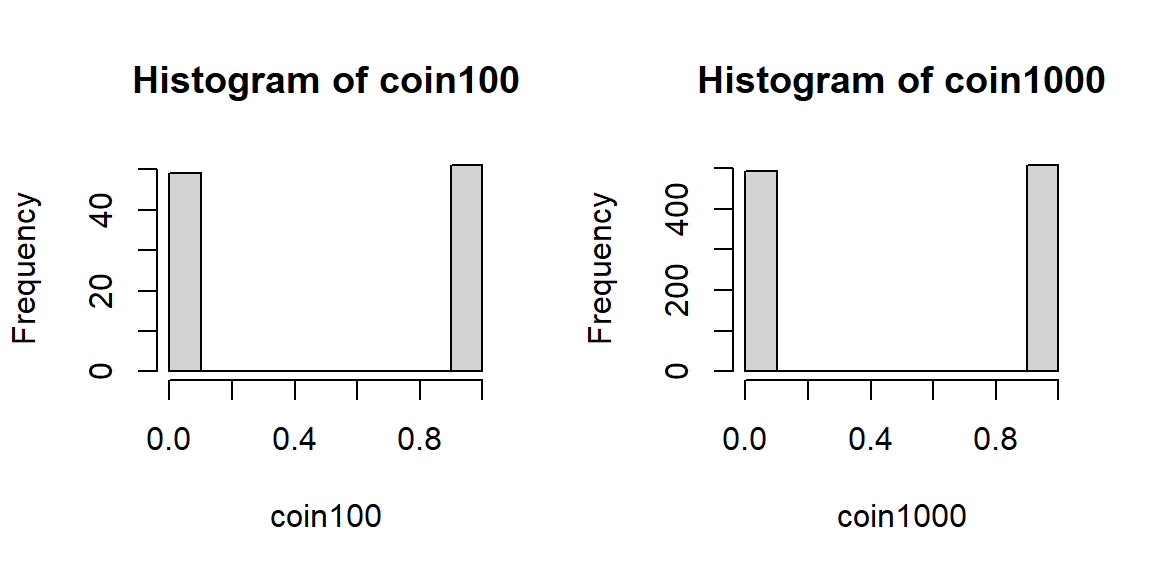
\includegraphics{Kor_BasicStats_files/figure-latex/unnamed-chunk-85-1} \end{center}

이와 같이 이항변수는 나뉘어진(discrete) 값을 가집니다. 히스토그램으로 그리면 0이 나오는 빈도랑 1이 나오는 빈도만 보여주는 것이지요. 이번에는 100개의 동전을 1000번 던지는 경우를 시뮬레이팅해보겠습니다.

\begin{Shaded}
\begin{Highlighting}[]
\NormalTok{coin1Mx <-}\StringTok{ }\KeywordTok{rep}\NormalTok{(}\OtherTok{NA}\NormalTok{, }\DecValTok{1000000}\NormalTok{)}
\ControlFlowTok{for}\NormalTok{(i }\ControlFlowTok{in} \DecValTok{1}\OperatorTok{:}\DecValTok{1000000}\NormalTok{)\{}
\NormalTok{coin1Mx[i] <-}\StringTok{ }\KeywordTok{sum}\NormalTok{(}\KeywordTok{rbinom}\NormalTok{(}\DecValTok{100}\NormalTok{, }\DecValTok{1}\NormalTok{, }\FloatTok{.5}\NormalTok{))}
\NormalTok{\}}
\KeywordTok{hist}\NormalTok{(coin1Mx, }
     \DataTypeTok{freq =} \OtherTok{FALSE}\NormalTok{, }
     \DataTypeTok{main =} \StringTok{"Distribution of heads}\CharTok{\textbackslash{}n}\StringTok{ in 100 coin tosses"}\NormalTok{, }
     \DataTypeTok{xlab =} \StringTok{"Number of heads"}\NormalTok{)}
\end{Highlighting}
\end{Shaded}

\begin{center}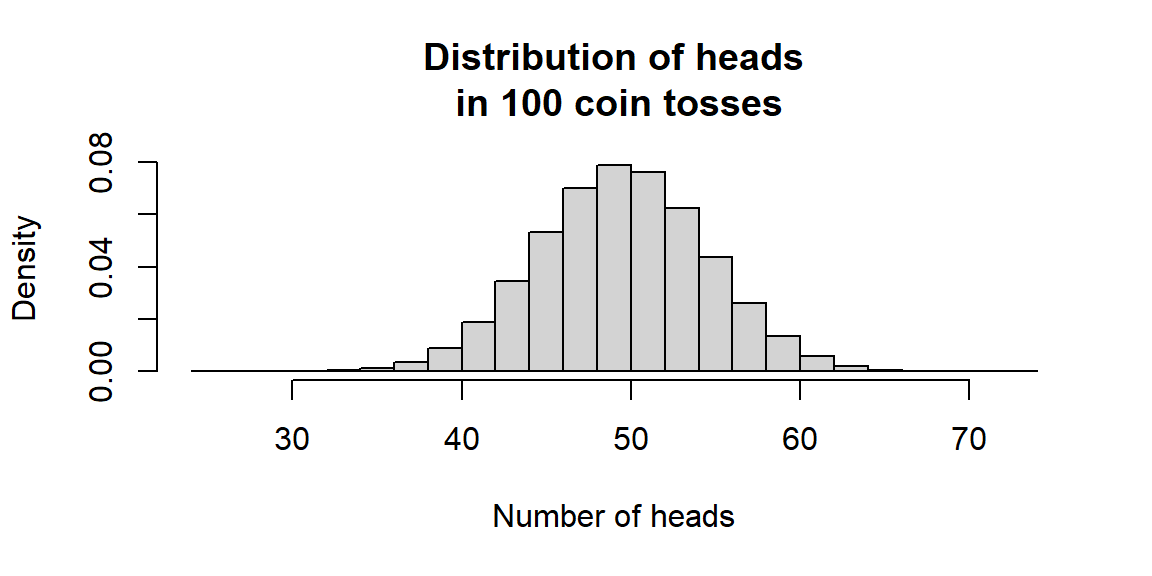
\includegraphics{Kor_BasicStats_files/figure-latex/unnamed-chunk-86-1} \end{center}

100만 개의 셀을 결측치(\texttt{NA})로 갖는 텅빈 \texttt{coinMx}라는 벡터를 만들어보겠습니다. 그리고 \texttt{i}가 1에서 100만까지 반복되는 \texttt{loop}를 구성합니다. \texttt{coin1Mx\_1}부터 \texttt{coin1Mx\_1000000}까지 총 100만개의 \texttt{coin1Mx\_n}들은 모두 100개의 동전을 던져서 앞면(1)이 나오는 경우의 수를 더한 각각의 값을 가질 것입니다. 따라서 \texttt{coin1Mx}는 100만개의 요소를 지닌 벡터입니다.

이 자료를 활용해서 만약 100개를 던졌을 때, 앞면이 60번 나오는 것이 과연 극단적인 확률일지 아니면 무던한 것일지 확인해보겠습니다자. 60번 이상 앞면이 나온 경우를 세는 함수를 짜보겠습니다.

\begin{Shaded}
\begin{Highlighting}[]
\KeywordTok{table}\NormalTok{(coin1Mx[coin1Mx }\OperatorTok{>}\StringTok{ }\DecValTok{60}\NormalTok{])}
\end{Highlighting}
\end{Shaded}

\begin{verbatim}
## 
##   61   62   63   64   65   66   67   68   69   70   71   72   74   75 
## 7070 4517 2763 1590  876  473  209  114   51   22   13    2    3    1
\end{verbatim}

\begin{Shaded}
\begin{Highlighting}[]
\NormalTok{coin1Mx[coin1Mx }\OperatorTok{>}\StringTok{ }\DecValTok{60}\NormalTok{] }\OperatorTok\StringTok{ }\KeywordTok{table}\NormalTok{() }\OperatorTok\StringTok{ }\KeywordTok{t}\NormalTok{() }\OperatorTok\StringTok{ }\KeywordTok{kable}\NormalTok{()}
\end{Highlighting}
\end{Shaded}

\begin{tabular}{r|r|r|r|r|r|r|r|r|r|r|r|r|r}
\hline
61 & 62 & 63 & 64 & 65 & 66 & 67 & 68 & 69 & 70 & 71 & 72 & 74 & 75\\
\hline
7070 & 4517 & 2763 & 1590 & 876 & 473 & 209 & 114 & 51 & 22 & 13 & 2 & 3 & 1\\
\hline
\end{tabular}

앞면이 나오는 빈도가 61번 이상부터는 점차 감소하는 것을 확인할 수 있습니다. 그렇다면 이번에는 앞면이 60번 넘게 나올 확률을 구해보겠습니다.

\begin{Shaded}
\begin{Highlighting}[]
\KeywordTok{length}\NormalTok{(coin1Mx[coin1Mx }\OperatorTok{>}\StringTok{ }\DecValTok{60}\NormalTok{])}\OperatorTok{/}\KeywordTok{length}\NormalTok{(coin1Mx)}
\end{Highlighting}
\end{Shaded}

\begin{verbatim}
## [1] 0.017704
\end{verbatim}

\begin{Shaded}
\begin{Highlighting}[]
\KeywordTok{sum}\NormalTok{(}\KeywordTok{table}\NormalTok{(coin1Mx[coin1Mx }\OperatorTok{>}\StringTok{ }\DecValTok{60}\NormalTok{]))}\OperatorTok{/}\DecValTok{1000000}
\end{Highlighting}
\end{Shaded}

\begin{verbatim}
## [1] 0.017704
\end{verbatim}

\texttt{length()}는 \texttt{count()}랑 같은 개념이라고 할 수 있습니다. 전체 \texttt{coin1Mx}의 수, 즉 100만 건 중에서 앞면이 60번보다 많이 나온 경우의 수가 어느 정도인지를 계산한 것입니다. 즉, 앞면이 60번보다 더 많이 나올 확률은 매우 작다고 할 수 있습니다다. 앞면이 60번 초과하여 나올 확률은 ``평균적'' or ``일반적''인 것은 아니라는 뜻입니다.

\hypertarget{uxb3c5uxb9bduxc0acuxac74-uxc2dcuxbbacuxb808uxc774uxc158}{%
\section{독립사건 시뮬레이션}\label{uxb3c5uxb9bduxc0acuxac74-uxc2dcuxbbacuxb808uxc774uxc158}}

두 개의 독립적인 사건을 시뮬레이션해보겠습니다. 첫 번째 함수는 \texttt{rand1}이라는 자료에 최소값 0, 최대값 10 미만의 값을 가지는 100개의 수를 무작위로 담으라는 명령입니다. 두 번째 함수는 정규분포를 따라 평균이 0이고 표준편차가 2의 값을 갖는 분포에서 100개의 값을 무작위로 추출해 rand2라는 자료에 담으라는 명령입니다.

\begin{itemize}
\tightlist
\item
  일단 보면 \texttt{rand2}의 경우, 비록 명령으로 평균을 0으로 하라고 설정했지만 무작위 추출 결과 100개의 값의 평균은 0보다 약간 큰 것을 확인할 수 있습니다.
\item
  이제 두 값을 각각 \texttt{x}축, \texttt{y}축으로 설정하여 100개의 값을 좌표에 매칭시킨 그래프로 나타내보겠습니다.
\end{itemize}

\begin{Shaded}
\begin{Highlighting}[]
\NormalTok{rand1 <-}\StringTok{ }\KeywordTok{runif}\NormalTok{(}\DecValTok{100}\NormalTok{, }\DataTypeTok{min =} \DecValTok{0}\NormalTok{, }\DataTypeTok{max =} \DecValTok{10}\NormalTok{)}
\KeywordTok{summary}\NormalTok{(rand1)}
\end{Highlighting}
\end{Shaded}

\begin{verbatim}
##    Min. 1st Qu.  Median    Mean 3rd Qu.    Max. 
##  0.2348  2.7605  4.7486  5.0535  7.6873  9.8271
\end{verbatim}

\begin{Shaded}
\begin{Highlighting}[]
\NormalTok{rand2 <-}\StringTok{ }\KeywordTok{rnorm}\NormalTok{(}\DecValTok{100}\NormalTok{, }\DataTypeTok{mean =} \DecValTok{0}\NormalTok{, }\DataTypeTok{sd =} \DecValTok{2}\NormalTok{)}
\KeywordTok{summary}\NormalTok{(rand2)}
\end{Highlighting}
\end{Shaded}

\begin{verbatim}
##     Min.  1st Qu.   Median     Mean  3rd Qu.     Max. 
## -4.42537 -1.66515 -0.06935 -0.09913  1.37622  5.83687
\end{verbatim}

\begin{Shaded}
\begin{Highlighting}[]
\KeywordTok{plot}\NormalTok{(rand1, rand2)}
\end{Highlighting}
\end{Shaded}

\begin{center}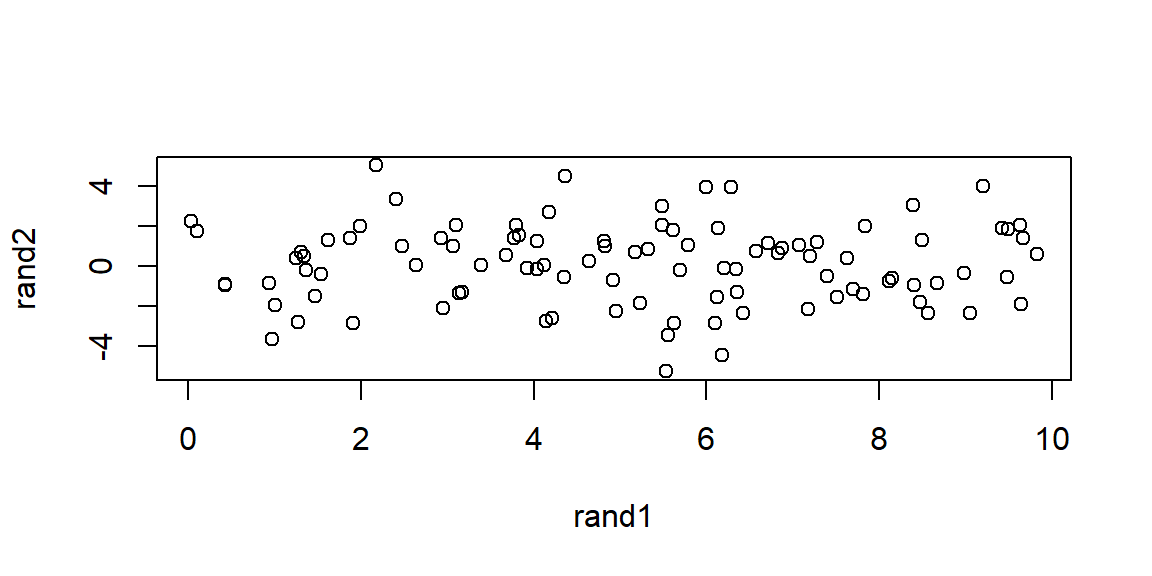
\includegraphics{Kor_BasicStats_files/figure-latex/unnamed-chunk-89-1} \end{center}

결과적으로 이 그래프에서 우리는 \texttt{rand1}과 \texttt{rand2} 간에는 어떠한 경향성을 발견하기 힘듭니다. 즉, 독립적이라는 것은 두 변수 간에 어떠한 관계를 상정할 수 없다는 것으로 이해할 수 있습니다.

\hypertarget{uxc885uxc18duxc0acuxac74-uxc2dcuxbbacuxb808uxc774uxc158}{%
\section{종속사건 시뮬레이션}\label{uxc885uxc18duxc0acuxac74-uxc2dcuxbbacuxb808uxc774uxc158}}

이번에는 두 사건이 종속적 관계에 있는, 즉 한 사건에서의 변화가 다른 사건에 영향을 미치는 경우를 시뮬레이션해 보겠습니다.

\begin{Shaded}
\begin{Highlighting}[]
\NormalTok{rand3 <-}\StringTok{ }\DecValTok{4} \OperatorTok{+}\StringTok{ }\FloatTok{0.75} \OperatorTok{*}\StringTok{ }\NormalTok{rand1 }\OperatorTok{+}\StringTok{ }\KeywordTok{rnorm}\NormalTok{(}\DecValTok{100}\NormalTok{, }\DataTypeTok{mean =} \DecValTok{0}\NormalTok{, }\DataTypeTok{sd =} \DecValTok{2}\NormalTok{)}
\end{Highlighting}
\end{Shaded}

\texttt{rand3}는 아까 만들어놓은 \texttt{rand1}에다가 0.75를 곱해서 4를 더한 100개의 값에다가 사실 상 \texttt{rand2}와 같은 방식으로 구한 값을 더하여 구한 자료입니다. 즉, 이 값은 \texttt{rand1}의 값에 어떠한 조치를 취하여 얻은 값이므로 \texttt{rand1}에 영향을 받은 결과물이라고 할 수 있습니다. 이렇게 구한 \texttt{rand3}와 \texttt{rand1} 간의 관계를 그래프로 나타내봅시다.

\begin{Shaded}
\begin{Highlighting}[]
\KeywordTok{plot}\NormalTok{(rand1, rand3)}
\end{Highlighting}
\end{Shaded}

\begin{center}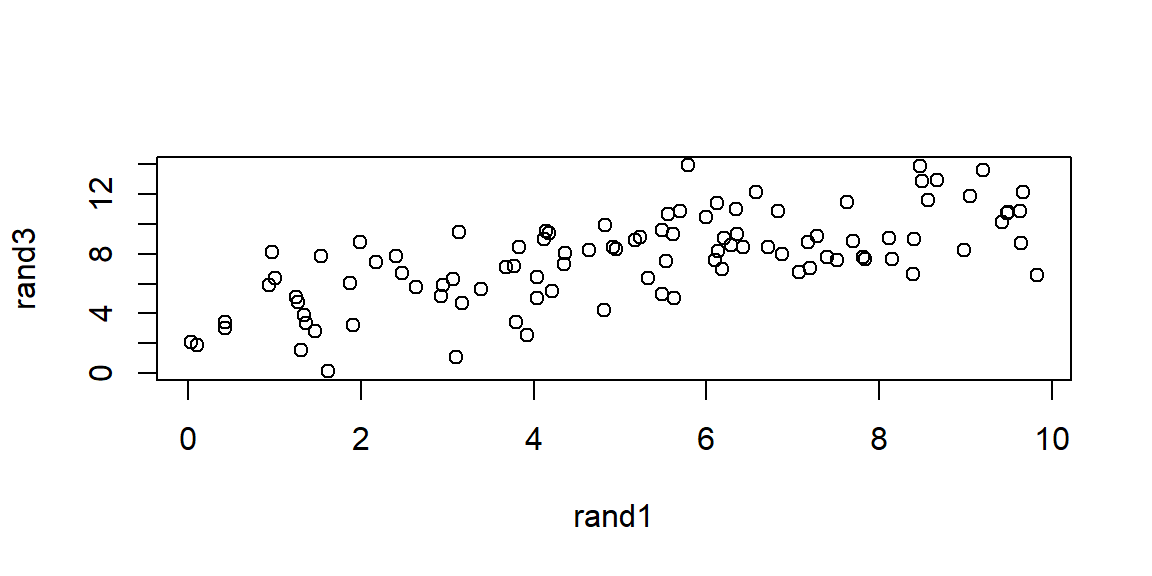
\includegraphics{Kor_BasicStats_files/figure-latex/unnamed-chunk-91-1} \end{center}

이 그래프의 해석은 나중에 산포도(scatter plot) 및 단순회귀분석(simple regression)을 살펴볼 때 다시 한 번 다룰 것입니다. 일단 여기서는 \texttt{rand1}이 증가할 때, \texttt{rand3}도 증가세를 보이는---둘의 인과적 관계는 확인할 수 없지만 아무튼---양(positive)의 관계를 보이고 있다는 것을 알 수 있습니다.

\texttt{cor(rand1,\ rand3)}로 두 변수 간의 상관계수를 구해보면\footnote{뒤의 \texttt{rnorm()}을 이용하여 무작위로 생성한 100개의 값을 구했기 때문에, 이 결과는 구할 때마다 달라질 것입니다.}, 양수의 기울기를 얻게 됩니다.

이번에는 보다 더 불확실성을 가지는 종속사건의 관계를 시뮬레이션해보겠습니다. 여기서 말하는 불확실성은 더 큰 표준편차를 의미합니다.

\begin{itemize}
\tightlist
\item
  표준편차가 평균에서 각 관측치가 떨어져 있는 거리의 평균이라고 할 때,
\item
  표준편차 값이 크다는 것은 개별 값들이 평균에서 더 넓게 분포해 있다는 것을 의미합니다.
\end{itemize}

\begin{Shaded}
\begin{Highlighting}[]
\NormalTok{rand4 <-}\StringTok{ }\DecValTok{4} \OperatorTok{+}\StringTok{ }\FloatTok{0.75} \OperatorTok{*}\StringTok{ }\NormalTok{rand1 }\OperatorTok{+}\StringTok{ }\KeywordTok{rnorm}\NormalTok{(}\DecValTok{100}\NormalTok{, }\DataTypeTok{mean =} \DecValTok{0}\NormalTok{, }\DataTypeTok{sd =} \DecValTok{5}\NormalTok{)}
\KeywordTok{plot}\NormalTok{(rand1, rand4)}
\end{Highlighting}
\end{Shaded}

\begin{center}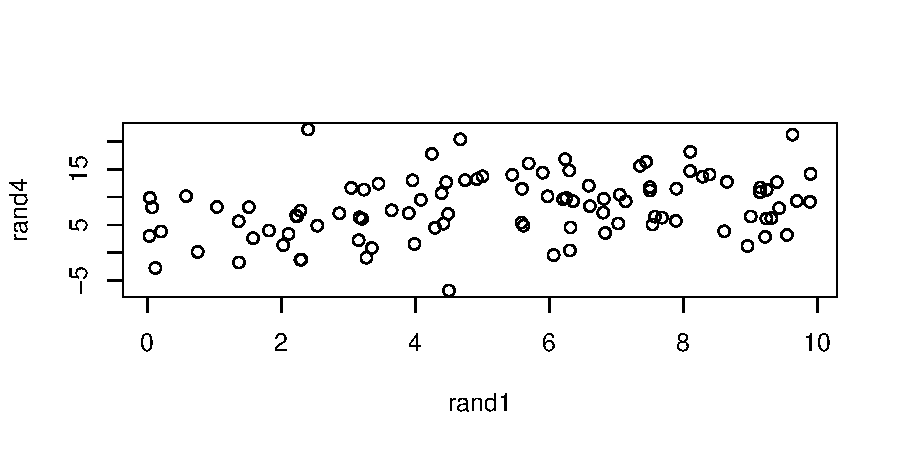
\includegraphics{Kor_BasicStats_files/figure-latex/unnamed-chunk-92-1} \end{center}

\begin{Shaded}
\begin{Highlighting}[]
\KeywordTok{cor}\NormalTok{(rand1, rand4)}
\end{Highlighting}
\end{Shaded}

\begin{verbatim}
## [1] 0.435429
\end{verbatim}

\texttt{rand1}과 \texttt{rand4}의 산포도는 좀 더 넓게 퍼진 모양새를 보이고 둘의 상관관계는 식에서 상정한 0.75라는 기울기에서 0.456으로 더 낮아지는 것을 확인할 수 있습니다.

\hypertarget{uxbd84uxd3ecdistribution}{%
\section{분포(Distribution)}\label{uxbd84uxd3ecdistribution}}

통계분석에 앞서서 일반적으로 알아두어야 할분포 함수(distribution functions)를 살펴보겠습니다. 먼저, 정규분포(normal distributions)와 이항분포(binomial distributions)로부터 분위(quantiles)를 얻어내는 방법을 살펴보겠습니다.

\hypertarget{uxc815uxaddcuxbd84uxd3ec-the-normal-distribution}{%
\subsection{정규분포 (The normal distribution)}\label{uxc815uxaddcuxbd84uxd3ec-the-normal-distribution}}

\begin{Shaded}
\begin{Highlighting}[]
\KeywordTok{pnorm}\NormalTok{(}\DecValTok{70}\NormalTok{, }\DataTypeTok{mean =} \DecValTok{50}\NormalTok{, }\DataTypeTok{sd =} \DecValTok{10}\NormalTok{, }\DataTypeTok{lower.tail =} \OtherTok{TRUE}\NormalTok{)}
\end{Highlighting}
\end{Shaded}

\begin{verbatim}
## [1] 0.9772499
\end{verbatim}

\begin{Shaded}
\begin{Highlighting}[]
\KeywordTok{pnorm}\NormalTok{(}\DecValTok{70}\NormalTok{, }\DataTypeTok{mean =} \DecValTok{50}\NormalTok{, }\DataTypeTok{sd =} \DecValTok{10}\NormalTok{, }\DataTypeTok{lower.tail =} \OtherTok{FALSE}\NormalTok{)}
\end{Highlighting}
\end{Shaded}

\begin{verbatim}
## [1] 0.02275013
\end{verbatim}

\begin{Shaded}
\begin{Highlighting}[]
\DecValTok{1} \OperatorTok{-}\StringTok{ }\KeywordTok{pnorm}\NormalTok{(}\DecValTok{70}\NormalTok{, }\DataTypeTok{mean =} \DecValTok{50}\NormalTok{, }\DataTypeTok{sd =} \DecValTok{10}\NormalTok{, }\DataTypeTok{lower.tail =} \OtherTok{TRUE}\NormalTok{)}
\end{Highlighting}
\end{Shaded}

\begin{verbatim}
## [1] 0.02275013
\end{verbatim}

첫번째 코드는 50을 평균으로 하고 10을 표준편차로 하는 정규분포가 있을 때, 그 분포에서 70이라는 숫자는 어디에 위치하는지를 묻는 것입니다.

두 번째도 동일한 의미인데, 두 식의 차이는 \texttt{lower.tail} 옵션을 어떻게 설정하느냐에 달려있습니다.

\begin{itemize}
\tightlist
\item
  각 식이 도출한 결과를 보면 이해하시겠지만 근본적으로 두 식은 동일하며, 좌측에서 누적확률을 계산할 것인지 우측으로부터 계산할 것인지의 차이일 뿐입니다.
\item
  간단하게 말하면 첫 번째 식은 70이라는 숫자는 이 분포에서 하위 97.7\%에 위치한 값이다라고 말하는 것이고 두 번째 식은 상위 2.2\%라고 말하는 것입니다.
\item
  따라서 두 번째 식은 전체 확률에서 첫 번째 식으로 계산한 확률을 제한 값과 같으므로 세 번째의 형태로 계산할 수도 있습니다.
\end{itemize}

그렇다면 만약에 양측꼬리 확률(two-tailed probability)에서 최소한 70만큼 `극단적인'(extreme) 확률을 얻고 싶을 때는 어떻게 해야할까요? 이 경우는 생각을 좀 달리 해보면 됩니다. 평균을 기점으로 70은 오른쪽 끝쪽에 위치하는 셈입니다. 그만큼 왼쪽 끝에 위치한 값을 상정하고 그 값이 나올 확률을 함께 계산해주어야 합니다.

이 경우 평균 50에서 70은 20만큼 떨어져 있습니다(우측으로, + 방향). 따라서 우리는 좌측으로 20만큼 떨어진 30이 나올 확률을 함께 고려해주어야 하는 것입니다. 이러한 결과를 얻는 데는두 가지 방법이 존재합니다.

\begin{Shaded}
\begin{Highlighting}[]
\CommentTok{## 첫 번째 방법}
\KeywordTok{pnorm}\NormalTok{(}\DecValTok{70}\NormalTok{, }\DataTypeTok{mean =} \DecValTok{50}\NormalTok{, }\DataTypeTok{sd =} \DecValTok{10}\NormalTok{, }\DataTypeTok{lower.tail =} \OtherTok{FALSE}\NormalTok{) }\OperatorTok{+}\StringTok{ }
\StringTok{  }\KeywordTok{pnorm}\NormalTok{(}\DecValTok{30}\NormalTok{, }\DataTypeTok{mean =} \DecValTok{50}\NormalTok{, }\DataTypeTok{sd =} \DecValTok{10}\NormalTok{, }\DataTypeTok{lower.tail =} \OtherTok{TRUE}\NormalTok{)}
\end{Highlighting}
\end{Shaded}

\begin{verbatim}
## [1] 0.04550026
\end{verbatim}

\begin{Shaded}
\begin{Highlighting}[]
\CommentTok{## 두 번째 방법}
\DecValTok{2} \OperatorTok{*}\StringTok{ }\KeywordTok{pnorm}\NormalTok{(}\DecValTok{70}\NormalTok{, }\DataTypeTok{mean =} \DecValTok{50}\NormalTok{, }\DataTypeTok{sd =} \DecValTok{10}\NormalTok{, }\DataTypeTok{lower.tail =} \OtherTok{FALSE}\NormalTok{)}
\end{Highlighting}
\end{Shaded}

\begin{verbatim}
## [1] 0.04550026
\end{verbatim}

그렇다면 이렇게 구한 분포에서의 누적확률 값을 가지고 분위를 구하여 보겠습니다. 마찬가지로 평균 50에 표준편차가 10인 분포를 상정합니다. 이때 사용할 함수는 \texttt{qnorm()}입니다.

\begin{Shaded}
\begin{Highlighting}[]
\KeywordTok{qnorm}\NormalTok{(}\FloatTok{0.9772499}\NormalTok{, }\DataTypeTok{mean =} \DecValTok{50}\NormalTok{, }\DataTypeTok{sd =} \DecValTok{10}\NormalTok{, }\DataTypeTok{lower.tail =} \OtherTok{TRUE}\NormalTok{)}
\end{Highlighting}
\end{Shaded}

\begin{verbatim}
## [1] 70.00001
\end{verbatim}

역으로 계산한 것인데, 평균 50에 표준편차 10인 분포에서 좌측부터 앞서 구한 누적확률에 해당하는 값을 구하라는 명령입니다. 앞에서 우리가 입력한 70과 근사한 값을 얻을 수 있습니다. 근소한 차이는 소수점에 의해 발생하는 것으로 이해하시면 됩니다.

다음으로는 주어진 평균 50, 표준편차 10의 분포에서 70이라는 값이 분포에서 차지하는 밀도를 확인해보겠습니다 밀도(density)를 알아보기 위한 함수는 다음과 같습니다.

\begin{Shaded}
\begin{Highlighting}[]
\KeywordTok{dnorm}\NormalTok{(}\DecValTok{70}\NormalTok{, }\DataTypeTok{mean =} \DecValTok{50}\NormalTok{, }\DataTypeTok{sd =} \DecValTok{10}\NormalTok{)}
\end{Highlighting}
\end{Shaded}

\begin{verbatim}
## [1] 0.005399097
\end{verbatim}

그렇다면 이번에는 정규분포에서 관측치를 무작위로 추출(draws)을 해보겠습니다. 이번에도 함수에는 70이라는 값이 사용될 것인데, 여기서 사용되는 70은 특정한 값이 아니라 추출 횟수를 의미합니다.

\begin{Shaded}
\begin{Highlighting}[]
\NormalTok{x <-}\StringTok{ }\KeywordTok{rnorm}\NormalTok{(}\DecValTok{70}\NormalTok{, }\DataTypeTok{mean =} \DecValTok{50}\NormalTok{, }\DataTypeTok{sd =} \DecValTok{10}\NormalTok{)}
\NormalTok{x}
\end{Highlighting}
\end{Shaded}

\begin{verbatim}
##  [1] 61.57291 45.23483 37.88554 40.09534 53.92205 33.80058 34.78782
##  [8] 40.49731 62.84562 38.68573 44.63655 28.66694 62.81471 65.31213
## [15] 40.39513 37.45665 58.92910 51.09220 64.23508 47.62329 57.35632
## [22] 46.17860 60.05903 47.10488 54.34855 71.61267 45.72614 40.34960
## [29] 52.14325 65.31368 54.66791 46.79477 55.07526 38.12352 57.81826
## [36] 67.99108 52.96645 37.97031 61.85548 60.79928 57.67317 36.95250
## [43] 54.96158 50.24880 45.66564 48.29958 54.62234 42.82173 56.15026
## [50] 43.69452 47.25371 37.40268 57.83976 59.97281 49.89494 51.54018
## [57] 60.07255 47.32968 61.89821 56.15981 60.79732 33.04195 53.43144
## [64] 43.49750 54.23114 59.57227 45.88471 43.87950 65.08663 43.33206
\end{verbatim}

총 70개의 값이 무작위로 추출되어 \texttt{x}라는 벡터에 담겨 있는 것을 확인할 수 있습니다.

이번에는 좀 더 구체적으로 정규분포 사례들을 살펴보겠습니다. 서로 다른 평균(mean)과 표준편차(standard deviation)를 가지는 세 개의 정규분포를 그려보겠습니다.

\begin{Shaded}
\begin{Highlighting}[]
\NormalTok{normal5 <-}\StringTok{ }\KeywordTok{rnorm}\NormalTok{(}\DataTypeTok{n =} \DecValTok{10000}\NormalTok{, }\DataTypeTok{mean =} \DecValTok{5}\NormalTok{, }\DataTypeTok{sd =} \DecValTok{3}\NormalTok{)}
\NormalTok{normal50 <-}\StringTok{ }\KeywordTok{rnorm}\NormalTok{(}\DataTypeTok{n =} \DecValTok{10000}\NormalTok{, }\DataTypeTok{mean =} \DecValTok{50}\NormalTok{, }\DataTypeTok{sd =} \DecValTok{10}\NormalTok{)}
\NormalTok{normal20 <-}\StringTok{ }\KeywordTok{rnorm}\NormalTok{(}\DataTypeTok{n =} \DecValTok{10000}\NormalTok{, }\DataTypeTok{mean =} \DecValTok{20}\NormalTok{, }\DataTypeTok{sd =} \DecValTok{1}\NormalTok{)}
\end{Highlighting}
\end{Shaded}

세 함수 모두 표본의 크기는 1만 개이며, 각자 다른 평균과 표준편차를 따르는 정규분포를 가정하여 무작위로 추출된 값을 담는 벡터로 출력됩니다. 이렇게 값을 갖는 세 개의 벡터를 하나의 데이터로 합쳐보겠습니다. 간단하게 말하면 하나의 표로 합친다는 것과 같습니다.

\begin{Shaded}
\begin{Highlighting}[]
\NormalTok{norm <-}\StringTok{ }\KeywordTok{bind_rows}\NormalTok{(}\KeywordTok{tibble}\NormalTok{(}\DataTypeTok{x =}\NormalTok{ normal5, }\DataTypeTok{Mean =} \DecValTok{5}\NormalTok{, }\DataTypeTok{SD =} \DecValTok{3}\NormalTok{),}
                  \KeywordTok{tibble}\NormalTok{(}\DataTypeTok{x =}\NormalTok{ normal50, }\DataTypeTok{Mean =} \DecValTok{50}\NormalTok{, }\DataTypeTok{SD =} \DecValTok{10}\NormalTok{),}
                  \KeywordTok{tibble}\NormalTok{(}\DataTypeTok{x =}\NormalTok{ normal20, }\DataTypeTok{Mean =} \DecValTok{20}\NormalTok{, }\DataTypeTok{SD =} \DecValTok{1}\NormalTok{))}
\NormalTok{norm}\OperatorTok{$}\NormalTok{Mean <-}\StringTok{ }\KeywordTok{as.factor}\NormalTok{(norm}\OperatorTok{$}\NormalTok{Mean)}
\end{Highlighting}
\end{Shaded}

그리고 이렇게 만들어진 데이터프레임의 평균 값을 \texttt{Factor} 자료 유형으로 변환해줍니다. 이것이 의미하는 게 뭘까요? 평균5, 평균50, 평균20을 문자열로 인식하게 하여 일종의 ``이름''으로 인식하게 만드는 것입니다. 그러면 이제 이렇게 만들어진 데이터로 그래프를 그려보겠습니다.

\begin{Shaded}
\begin{Highlighting}[]
\KeywordTok{ggplot}\NormalTok{(norm, }\KeywordTok{aes}\NormalTok{(}\DataTypeTok{x =}\NormalTok{ x)) }\OperatorTok{+}
\StringTok{  }\KeywordTok{geom_density}\NormalTok{(}\KeywordTok{aes}\NormalTok{(}\DataTypeTok{fill =} \KeywordTok{as.factor}\NormalTok{(Mean)), }\DataTypeTok{adjust =} \DecValTok{4}\NormalTok{, }\DataTypeTok{alpha =} \DecValTok{1}\OperatorTok{/}\DecValTok{2}\NormalTok{) }\OperatorTok{+}
\StringTok{  }\KeywordTok{guides}\NormalTok{(}\DataTypeTok{color=}\KeywordTok{guide_legend}\NormalTok{(}\DataTypeTok{title =} \StringTok{"Mean, SD"}\NormalTok{)) }\OperatorTok{+}
\StringTok{  }\KeywordTok{guides}\NormalTok{(}\DataTypeTok{fill=}\KeywordTok{guide_legend}\NormalTok{(}\DataTypeTok{title =} \StringTok{"Mean, SD"}\NormalTok{)) }\OperatorTok{+}
\StringTok{  }\KeywordTok{scale_color_discrete}\NormalTok{(}\DataTypeTok{labels =} \KeywordTok{c}\NormalTok{(}\StringTok{"5, 3"}\NormalTok{, }\StringTok{"20, 1"}\NormalTok{, }\StringTok{"50, 10"}\NormalTok{)) }\OperatorTok{+}
\StringTok{  }\KeywordTok{scale_fill_discrete}\NormalTok{(}\DataTypeTok{labels =} \KeywordTok{c}\NormalTok{(}\StringTok{"5, 3"}\NormalTok{, }\StringTok{"20, 1"}\NormalTok{, }\StringTok{"50, 10"}\NormalTok{)) }\OperatorTok{+}
\StringTok{  }\KeywordTok{ggtitle}\NormalTok{(}\StringTok{"Probability Density Function}\CharTok{\textbackslash{}n}\StringTok{Normal Distribution"}\NormalTok{)}
\end{Highlighting}
\end{Shaded}

\begin{center}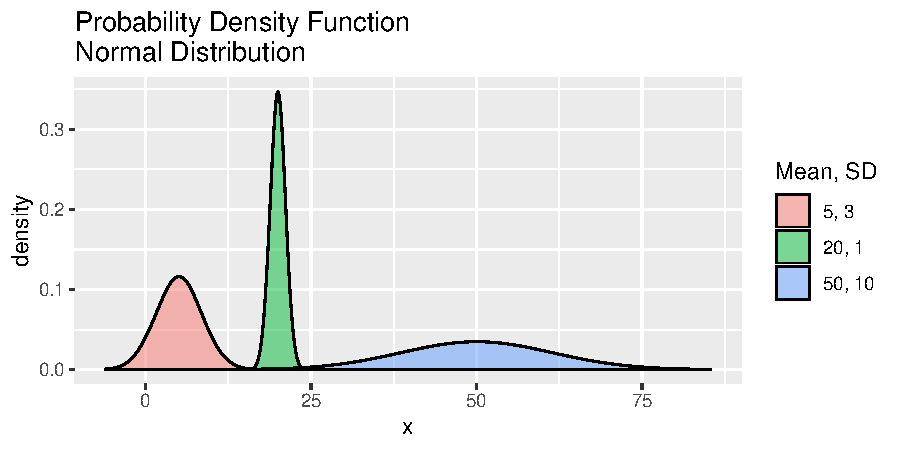
\includegraphics{Kor_BasicStats_files/figure-latex/unnamed-chunk-100-1} \end{center}

\texttt{ggplot2} 패키지는 \textbf{R}에서 그래프를 그리는 데 있어서 유용하게 사용됩니다. 먼저 \texttt{ggplot2} 패키지를 불러오고 나서, \texttt{ggplot(데이터프레임\ 이름,\ aes(x\ =\ x축으로\ 삼을\ 변수이름))}을 설정하면 일단 수학적으로 지정한 데이터의 변수에 대한 기본적인 작업은 진행이 됩니다.

그러나 이 단계에서는 아직 가시화(visualization)라고 할 수는 없는데, 주어진 데이터를 컴퓨팅했을 뿐이지 어떻게 가시적인 형태로 보여주라는 명령을 부여하지 않았기 때문입니다. 컴퓨터로 그림을 그려본 사람들은 이해가 쉬운데, \texttt{ggplot()}은 레이어 시스템을 이용해서, 우리가 뭔가 그려진 걸 얻고 싶을 때마다 레이어를 하나씩 추가해서 보여달라고 \textbf{R}에게 요구해야만 합니다.

그리고 이때, 레이어를 추가하는 것은 \texttt{+}로 가능합니다. 하나씩 뜯어서 보면,

\begin{itemize}
\tightlist
\item
  \texttt{ggplot(norm,\ aes(x\ =\ x))\ +} : \texttt{ggplot2} 패키지를 이용하여 \texttt{norm}이라는 데이터 프레임에서 \texttt{x}축에는 \texttt{x}라는 변수를 기준으로 늘어놓아라. 그리고 뒤에 더해지는 레이어 명령을 덮어 씌워라 라는 의미의 코드입니다.
\item
  \texttt{geom\_density(aes(fill\ =\ as.factor(Mean)),\ adjust\ =\ 4,\ alpha\ =\ 1/2)\ +}: 밀도함수의 형태로 그래프를 그리되, \texttt{Mean}이라는 \texttt{Factor} 변수가 같은 것들 끼리 같은 색으로 칠해서 보여주어라 라는 코드입니다.

  \begin{itemize}
  \tightlist
  \item
    뒤의 옵션은 세세한 조정이니 굳이 언급하지는 겠습니다.
  \item
    뒤에 더해지는 옵션들은 레이어를 추가하여 기존의 코드에 덮어 씌워, 그래프를 덧칠하는 역할을 합니다.
  \end{itemize}
\item
  \texttt{guides(color=guide\_legend(title\ =\ "Mean,\ SD"))\ +\ guides(fill=guide\_legend(title\ =\ "Mean,\ SD"))\ +}: 우측에 더해지는 레전드의 이름을 어떻게 지으라는 명령입니다.

  \begin{itemize}
  \tightlist
  \item
    이 경우에는 색도 있고 그래프를 선명하게 보여주는 선도 있기 때문에 그 각각이 레이어를 이루고 있어 둘 모두에게 이러한 명령어를 적용해야 합니다.
  \end{itemize}
\item
  \texttt{scale\_color\_discrete(labels\ =\ c("5,\ 3",\ "20,\ 1",\ "50,\ 10"))\ +\ \ scale\_fill\_discrete(labels\ =\ c("5,\ 3",\ "20,\ 1",\ "50,\ 10"))\ +}: \texttt{color}와 \texttt{fill}을 뒤에 이어지를 라벨로 구분해주라는 코드입니다.
\item
  ggtitle(\texttt{Probability\ Density\ Function\textbackslash{}nNormal\ Distribution}) : 표 전체의 이름을 지정하는 명령어이고, \texttt{\textbackslash{}n}은 \textbf{R}에서는 강제 개행(enter)하는 명령어입니다.
\end{itemize}

\hypertarget{uxc774uxd56duxbd84uxd3ec-binomial-distribution}{%
\subsection{이항분포 (Binomial distribution)}\label{uxc774uxd56duxbd84uxd3ec-binomial-distribution}}

이항분포는 우리에게 \texttt{n}번의 시행에서 \texttt{k}번 성공할 확률을 보여주는 분포입니다. 단순하게 말하자면 0과 1의 값만 갖는다고 가정된 벡터가 있다고 하겠습니다. 이때 벡터의 요소의 총 개수는 100개이고 랜덤으로 0과 1 중 하나가 벡터에 들어간다고 할 수 있습니다. 이때 전체 요소의 수 100개 중 1이 뽑혔을 경우를 계산하면 결국 1을 뽑을 성공 사례의 총합을 100으로 나눔으로써, 전체 대비 성공의 확률을 구하는 것이라 할 수 있습니다. 즉, 정규분포에서와는 다르게 이항분포에서는 평균(mean)이 아니라 비율(proportion)에 초점을 맞추게 됩니다.

\begin{Shaded}
\begin{Highlighting}[]
\KeywordTok{pbinom}\NormalTok{(}\DecValTok{27}\NormalTok{, }\DataTypeTok{size=}\DecValTok{100}\NormalTok{, }\DataTypeTok{prob=}\FloatTok{0.25}\NormalTok{, }\DataTypeTok{lower.tail =} \OtherTok{TRUE}\NormalTok{)}
\end{Highlighting}
\end{Shaded}

\begin{verbatim}
## [1] 0.7223805
\end{verbatim}

시도가 성공할 확률을 0.25라고 놓고 시행 횟수를 100번으로 가정한 경우입니다. 즉, 100번 시도했을 때 성공할 확률이 25\%인 이항분포를 가지는 데, 실제로는 27번 성공했다고 한다면 누적확률에서 어느 위치에 해당하는지를 묻는 함수입니다. \texttt{lower.tail()}이 \texttt{TRUE}로 설정되어 있으므로 좌측에서부터 계산한 것입니다. 즉, 27번 성공한 것은 하위 72.2\%, 상위 27.8\%에 해당한다는 것을 알 수 있습니다.

\begin{Shaded}
\begin{Highlighting}[]
\KeywordTok{qbinom}\NormalTok{(}\FloatTok{0.7223805}\NormalTok{, }\DataTypeTok{size =} \DecValTok{100}\NormalTok{, }\DataTypeTok{prob =} \FloatTok{0.25}\NormalTok{, }\DataTypeTok{lower.tail =} \OtherTok{TRUE}\NormalTok{)}
\end{Highlighting}
\end{Shaded}

\begin{verbatim}
## [1] 27
\end{verbatim}

이렇게 구한 누적확률로 다시금 성공 횟수를 추정해보겠습니다. 정규분포때와 거의 유사합니다. \texttt{size\ =\ 100}은 서로 독립적인 사건의 시행, 즉 베르누이 시행(Bernoulli trials)의 횟수를 의미합니다. 그렇다면 100번 시도했을 때 27번 성공할 정확한 확률을 구해보겠습니다.

\begin{Shaded}
\begin{Highlighting}[]
\KeywordTok{dbinom}\NormalTok{(}\DecValTok{27}\NormalTok{, }\DataTypeTok{size=}\DecValTok{100}\NormalTok{, }\DataTypeTok{prob=}\FloatTok{0.25}\NormalTok{)}
\end{Highlighting}
\end{Shaded}

\begin{verbatim}
## [1] 0.08064075
\end{verbatim}

\begin{Shaded}
\begin{Highlighting}[]
\KeywordTok{choose}\NormalTok{(}\DecValTok{100}\NormalTok{, }\DecValTok{27}\NormalTok{)}\OperatorTok{*}\NormalTok{.}\DecValTok{25}\OperatorTok{^}\DecValTok{27}\OperatorTok{*}\NormalTok{(}\DecValTok{1}\FloatTok{-.25}\NormalTok{)}\OperatorTok{^}\NormalTok{(}\DecValTok{100-27}\NormalTok{)}
\end{Highlighting}
\end{Shaded}

\begin{verbatim}
## [1] 0.08064075
\end{verbatim}

두 가지 방법으로 구할 수 있는데, 첫 번째는 \textbf{R}에 내장된 기본 함수인 \texttt{dbinom()}으로 구하는 것입니다. 두 번째는 \texttt{choose()} 함수를 이용해서 구하는 것입니다. 개인적으로는 \texttt{dbinom()} 함수가 있는데 굳이 \texttt{choose()} 함수 사용법까지 알아야 하나 싶기는 합니다. 그러나 \texttt{choose()} 함수로 보여지는 식이 좀 더 직관적으로 이해하기에는 도움이 됩니다.

\begin{Shaded}
\begin{Highlighting}[]
\KeywordTok{rbinom}\NormalTok{(}\DecValTok{27}\NormalTok{, }\DataTypeTok{size=}\DecValTok{100}\NormalTok{, }\DataTypeTok{prob=}\FloatTok{0.25}\NormalTok{)}
\end{Highlighting}
\end{Shaded}

\begin{verbatim}
##  [1] 18 27 20 25 23 19 23 24 22 28 31 27 25 20 31 27 19 23 28 22 24 16 28
## [24] 26 15 28 26
\end{verbatim}

\begin{Shaded}
\begin{Highlighting}[]
\KeywordTok{sd}\NormalTok{(}\KeywordTok{rbinom}\NormalTok{(}\DecValTok{27}\NormalTok{, }\DataTypeTok{size=}\DecValTok{100}\NormalTok{, }\DataTypeTok{prob=}\FloatTok{0.25}\NormalTok{))}
\end{Highlighting}
\end{Shaded}

\begin{verbatim}
## [1] 3.818906
\end{verbatim}

마지막으로는 0.25의 확률을 가진 100번의 베르누이 시행을 27번을 반복하는 결과를 보여줍니다. 즉, 평균적으로는 100번 시행 중 25번의 성공을 할 것으로 기대되지만, 실제 시행을 27번 해보면 무작위 추출이기 때문에 25를 중심으로 표준편차 4.21의 범위 내에서 여러 값들이 추출되는 것을 확인할 수 있습니다. 무작위로 추출하기 때문에 돌릴 때마다 값은 다르게 나올 것입니다.

다시 한 번, \texttt{n}번의 독립적인 베르누이 사건을 시행할 때, \texttt{k}번 성공할 확률을 구하는 이항분포로 실습해보겠습니다. 구체적으로 모집단의 성공 확률을 \texttt{p}, 모집단의 크기를 \texttt{n}으로 특정하겠습니다.

\begin{Shaded}
\begin{Highlighting}[]
\NormalTok{binom10 <-}\StringTok{ }\KeywordTok{rbinom}\NormalTok{(}\DataTypeTok{n =} \DecValTok{10000}\NormalTok{, }\DataTypeTok{p =} \FloatTok{.5}\NormalTok{, }\DataTypeTok{size =} \DecValTok{10}\NormalTok{)}
\NormalTok{binom50 <-}\StringTok{ }\KeywordTok{rbinom}\NormalTok{(}\DataTypeTok{n =} \DecValTok{10000}\NormalTok{, }\DataTypeTok{p =} \FloatTok{.5}\NormalTok{, }\DataTypeTok{size =} \DecValTok{50}\NormalTok{)}
\NormalTok{binom100 <-}\StringTok{ }\KeywordTok{rbinom}\NormalTok{(}\DataTypeTok{n =} \DecValTok{10000}\NormalTok{, }\DataTypeTok{p =} \FloatTok{.5}\NormalTok{, }\DataTypeTok{size =} \DecValTok{100}\NormalTok{)}
\end{Highlighting}
\end{Shaded}

정규분포와 다르지는 않습니다. 다만 여기서의 \texttt{size}는 전체 동전을 던지는 횟수로 이해하면 되고 10,000은 그렇게 동전을 10번, 50번, 100번 던지는 걸 10,000번 반복한다는 의미라고 할 수 있습니다. 그럼 이제 마찬가지로 하나의 데이터프레임으로 세 번의 시도(\texttt{binom10}, \texttt{binom50}, \texttt{binom100})의 결과를 합쳐주고 그래프를 그려보겠습니다.

\begin{Shaded}
\begin{Highlighting}[]
\NormalTok{binom <-}\StringTok{ }\KeywordTok{bind_rows}\NormalTok{(}\KeywordTok{tibble}\NormalTok{(}\DataTypeTok{k =}\NormalTok{ binom10, }\DataTypeTok{Size =} \DecValTok{10}\NormalTok{), }
                   \KeywordTok{tibble}\NormalTok{(}\DataTypeTok{k =}\NormalTok{ binom50, }\DataTypeTok{Size =} \DecValTok{50}\NormalTok{), }
                   \KeywordTok{tibble}\NormalTok{(}\DataTypeTok{k =}\NormalTok{ binom100, }\DataTypeTok{Size =} \DecValTok{100}\NormalTok{))}
\NormalTok{binom}\OperatorTok{$}\NormalTok{Size <-}\StringTok{ }\KeywordTok{as.factor}\NormalTok{(binom}\OperatorTok{$}\NormalTok{Size)}

\KeywordTok{ggplot}\NormalTok{(binom, }\KeywordTok{aes}\NormalTok{(}\DataTypeTok{x =}\NormalTok{ k)) }\OperatorTok{+}
\StringTok{  }\KeywordTok{geom_density}\NormalTok{(}\KeywordTok{aes}\NormalTok{(}\DataTypeTok{group =}\NormalTok{ Size, }\DataTypeTok{color =}\NormalTok{ Size, }\DataTypeTok{fill =}\NormalTok{ Size), }
               \DataTypeTok{adjust =} \DecValTok{4}\NormalTok{, }\DataTypeTok{alpha =} \DecValTok{1}\OperatorTok{/}\DecValTok{2}\NormalTok{) }\OperatorTok{+}
\StringTok{  }\KeywordTok{ggtitle}\NormalTok{(}\StringTok{"Probability Mass Function}\CharTok{\textbackslash{}n}\StringTok{Binomial Distribution"}\NormalTok{)}
\end{Highlighting}
\end{Shaded}

\begin{center}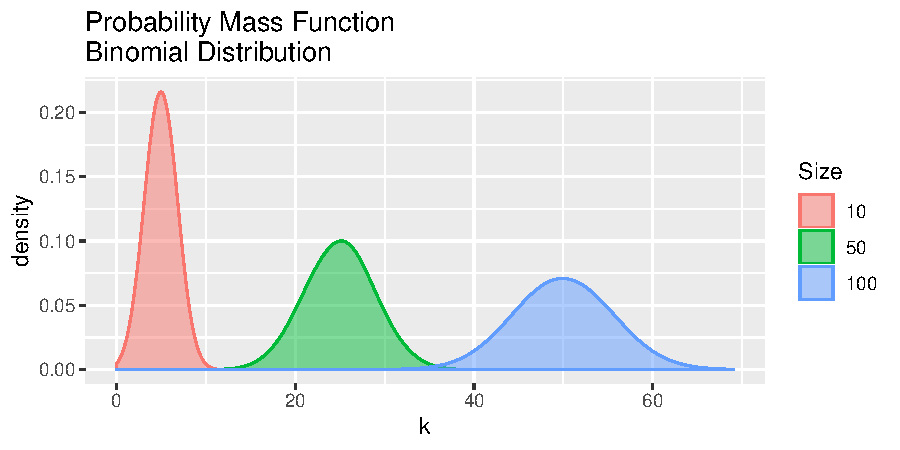
\includegraphics{Kor_BasicStats_files/figure-latex/unnamed-chunk-106-1} \end{center}

\hypertarget{uxd3ecuxc640uxc1a1-uxbd84uxd3ec-poison-distribution}{%
\subsection{포와송 분포 (Poison distribution)}\label{uxd3ecuxc640uxc1a1-uxbd84uxd3ec-poison-distribution}}

이 포스팅은 주로 \textbf{R} 코드에 관한 것이기 때문에 분포에 대한 수리통계적인 설명은 가급적 피하도록 하겠습니다. 포와송 분포는 고정된 대규모 모집단(fixed large population)에서 짧은 시간에 걸쳐서 희소한 사건(rare events)의 발생 횟수를 추정하는 데 용이한 분포입니다.

포와송 분포에서 그 희소한 사건의 발생 확률은 시간 단위 별 발생의 평균 횟수로 나타나며 그리스어 람다(\texttt{Lambda}, \(\lambda\))로 표기됩니다. 람다는 평균과 분산을 결정합니다.

포와송 분포의 확률을 이용해서 우리는 단일 시간 단위에서 \texttt{k}라는 희소한 사건을 정확하게 관측할 확률을 기술할 수 있습니다. 나머지는 앞의 정규분포랑 이항분포에서 했던 코드를 기계적으로 반복해서 살펴보는 것과 같습니자. 단, 포와송 분포에서 코드 중에는 이전과 다른 부분이 있으니 그 점만 유의하면 될 것 같습니다.

\begin{Shaded}
\begin{Highlighting}[]
\NormalTok{pois1 <-}\StringTok{ }\KeywordTok{rpois}\NormalTok{(}\DataTypeTok{n =} \DecValTok{10000}\NormalTok{, }\DataTypeTok{lambda =} \DecValTok{1}\NormalTok{)}
\NormalTok{pois2 <-}\StringTok{ }\KeywordTok{rpois}\NormalTok{(}\DataTypeTok{n =} \DecValTok{10000}\NormalTok{, }\DataTypeTok{lambda =} \DecValTok{2}\NormalTok{)}
\NormalTok{pois5 <-}\StringTok{ }\KeywordTok{rpois}\NormalTok{(}\DataTypeTok{n =} \DecValTok{10000}\NormalTok{, }\DataTypeTok{lambda =} \DecValTok{5}\NormalTok{)}
\NormalTok{pois20 <-}\StringTok{ }\KeywordTok{rpois}\NormalTok{(}\DataTypeTok{n =} \DecValTok{10000}\NormalTok{, }\DataTypeTok{lambda =} \DecValTok{20}\NormalTok{)}
\NormalTok{pois <-}\StringTok{ }\KeywordTok{tibble}\NormalTok{(}\DataTypeTok{Lambda.1 =}\NormalTok{ pois1, }
               \DataTypeTok{Lamnda.2 =}\NormalTok{ pois2,}
               \DataTypeTok{Lambda.5 =}\NormalTok{ pois5,}
               \DataTypeTok{Lambda.20 =}\NormalTok{ pois20)}
\end{Highlighting}
\end{Shaded}

이번에는 만들어진 \texttt{pois}라는 데이터를 \texttt{melt()} 함수를 이용해서 다른 변수로 재구성해줄 것입니다. \texttt{melt()} 함수는 \texttt{reshape2} 패키지에서 로드할 수 있고, \texttt{str\_extract()} 함수는 \texttt{stringr} 패키지에서 로드할 수 있다.

\begin{Shaded}
\begin{Highlighting}[]
\KeywordTok{library}\NormalTok{(reshape2)}
\KeywordTok{library}\NormalTok{(stringr)}
\NormalTok{pois <-}\StringTok{ }\KeywordTok{melt}\NormalTok{(}\DataTypeTok{data =}\NormalTok{ pois, }
             \DataTypeTok{variable.name =} \StringTok{"Lambda"}\NormalTok{, }
             \DataTypeTok{value.name =} \StringTok{"x"}\NormalTok{)}
\NormalTok{pois}\OperatorTok{$}\NormalTok{Lambda <-}\StringTok{ }
\StringTok{  }\KeywordTok{as.factor}\NormalTok{(}\KeywordTok{as.numeric}\NormalTok{(}\KeywordTok{str_extract}\NormalTok{(}\DataTypeTok{string =} 
\NormalTok{                                     pois}\OperatorTok{$}\NormalTok{Lambda, }
                                   \DataTypeTok{pattern =} \StringTok{"}\CharTok{\textbackslash{}\textbackslash{}}\StringTok{d+"}\NormalTok{)))}
\end{Highlighting}
\end{Shaded}

아래 그림에서 맨 왼쪽은 처음 만들어진 \texttt{pois} 데이터입니다. 두 번째는 \texttt{melt()} 함수를 이용해서 \texttt{Lambda}라는 변수 아래에 1, 2, 3, 4의 라벨을 길게(long-shape) 합친 것입니다. 그리고 마지막으로는 \texttt{Lambda} 변수의 문자열 \texttt{Lambda.}을 제외한 라벨 숫자만 남겨놓은 것입니다.

\begin{longtable}[]{@{}ccc@{}}
\toprule
\texttt{pois} 데이터 & \texttt{long-shaped\ pois} & \texttt{label\ only}\tabularnewline
\midrule
\endhead
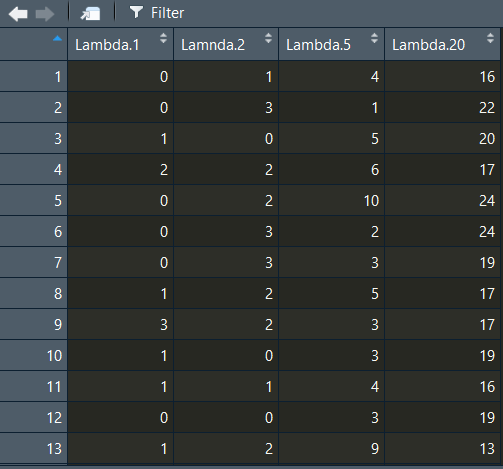
\includegraphics{r.post/pois1.png} & 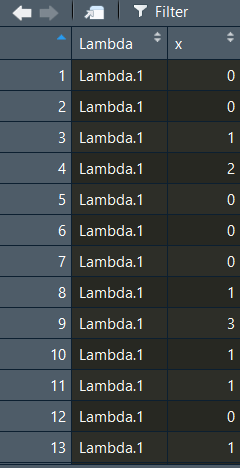
\includegraphics{r.post/pois2.png} & 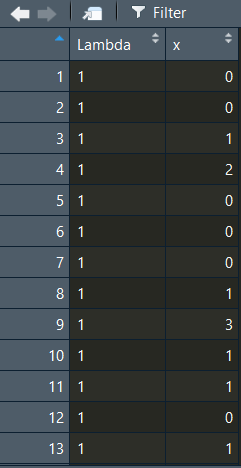
\includegraphics{r.post/pois3.png}\tabularnewline
\bottomrule
\end{longtable}

이렇게 만들어진 포와송 분포의 값들을 하나의 그래프로 만들어서 가시화해볼 수도 있습니다.

\begin{Shaded}
\begin{Highlighting}[]
\KeywordTok{ggplot}\NormalTok{(pois, }\KeywordTok{aes}\NormalTok{(}\DataTypeTok{x =}\NormalTok{ x)) }\OperatorTok{+}
\StringTok{  }\KeywordTok{geom_density}\NormalTok{(}\KeywordTok{aes}\NormalTok{(}\DataTypeTok{group =}\NormalTok{ Lambda, }
                   \DataTypeTok{color =}\NormalTok{ Lambda, }
                   \DataTypeTok{fill =}\NormalTok{ Lambda), }
               \DataTypeTok{adjust =} \DecValTok{4}\NormalTok{, }\DataTypeTok{alpha =} \DecValTok{1}\OperatorTok{/}\DecValTok{2}\NormalTok{) }\OperatorTok{+}
\StringTok{  }\KeywordTok{ggtitle}\NormalTok{(}\StringTok{"Probability Mass Function}\CharTok{\textbackslash{}n}\StringTok{Poisson Distribution"}\NormalTok{)}
\end{Highlighting}
\end{Shaded}

\begin{center}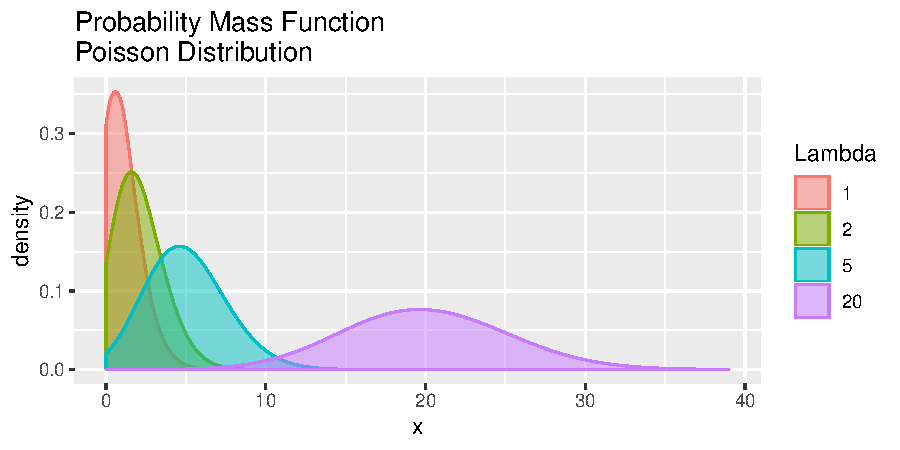
\includegraphics{Kor_BasicStats_files/figure-latex/unnamed-chunk-109-1} \end{center}

\hypertarget{uxc74cuxc774uxd56d-uxbd84uxd3ec-negative-binomial-distribution}{%
\subsection{음이항 분포 (Negative Binomial Distribution)}\label{uxc74cuxc774uxd56d-uxbd84uxd3ec-negative-binomial-distribution}}

음이항 분포는 \texttt{n}번째 시도에서 \texttt{k}번째에 성공할 확률을 보여줍니다. 음이항 분포는 다음과 같은 네 조건이 충족될 때 유용합니다.

\begin{enumerate}
\def\labelenumi{\arabic{enumi}.}
\tightlist
\item
  모든 시도는 독립적이다.
\item
  각 시도의 결과는 성공 혹은 실패로 구분될 수 있다.
\item
  성공 확률 (\texttt{p})은 각 시도마다 동일하다.
\item
  마지막 시도는 항상 성공이어야만 한다.
\end{enumerate}

여기서 보면 알 수 있듯이, 처음 세 조건은 이항분포와 동일합니다. 세 개의 음이항 분포 결과를 계산하여 세 개의 벡터로 저장하겠습니다. 그리고 이걸 마찬가지로 하나의 데이터로 합칩니다.

\begin{Shaded}
\begin{Highlighting}[]
\NormalTok{nbinom1 <-}\StringTok{ }\KeywordTok{rnbinom}\NormalTok{(}\DataTypeTok{n =} \DecValTok{10000}\NormalTok{, }\DataTypeTok{p =} \FloatTok{.3}\NormalTok{, }\DataTypeTok{size =} \DecValTok{1}\NormalTok{)}
\NormalTok{nbinom5 <-}\StringTok{ }\KeywordTok{rnbinom}\NormalTok{(}\DataTypeTok{n =} \DecValTok{10000}\NormalTok{, }\DataTypeTok{p =} \FloatTok{.3}\NormalTok{, }\DataTypeTok{size =} \DecValTok{5}\NormalTok{)}
\NormalTok{nbinom10 <-}\StringTok{ }\KeywordTok{rnbinom}\NormalTok{(}\DataTypeTok{n =} \DecValTok{10000}\NormalTok{, }\DataTypeTok{p =} \FloatTok{.3}\NormalTok{, }\DataTypeTok{size =} \DecValTok{10}\NormalTok{)}
\NormalTok{nbinom <-}\StringTok{ }\KeywordTok{bind_rows}\NormalTok{(}\KeywordTok{tibble}\NormalTok{(}\DataTypeTok{x =}\NormalTok{ nbinom1, }\DataTypeTok{Size =} \DecValTok{1}\NormalTok{), }
                    \KeywordTok{tibble}\NormalTok{(}\DataTypeTok{x =}\NormalTok{ nbinom5, }\DataTypeTok{Size =} \DecValTok{5}\NormalTok{), }
                    \KeywordTok{tibble}\NormalTok{(}\DataTypeTok{x =}\NormalTok{ nbinom10, }\DataTypeTok{Size =} \DecValTok{10}\NormalTok{))}
\NormalTok{nbinom}\OperatorTok{$}\NormalTok{Size <-}\StringTok{ }\KeywordTok{as.factor}\NormalTok{(nbinom}\OperatorTok{$}\NormalTok{Size)}
\end{Highlighting}
\end{Shaded}

포와송이랑 이항분포에서 사용했던 함수들과 거의 유사합니다. 이렇게 만들어진 그래프는 다음과 같습니다.

\begin{Shaded}
\begin{Highlighting}[]
\KeywordTok{ggplot}\NormalTok{(nbinom, }\KeywordTok{aes}\NormalTok{(}\DataTypeTok{x =}\NormalTok{ x)) }\OperatorTok{+}
\StringTok{  }\KeywordTok{geom_density}\NormalTok{(}\KeywordTok{aes}\NormalTok{(}\DataTypeTok{group =}\NormalTok{ Size, }\DataTypeTok{color =}\NormalTok{ Size, }\DataTypeTok{fill =}\NormalTok{ Size), }
               \DataTypeTok{adjust =} \DecValTok{4}\NormalTok{, }\DataTypeTok{alpha =} \DecValTok{1}\OperatorTok{/}\DecValTok{2}\NormalTok{) }\OperatorTok{+}
\StringTok{  }\KeywordTok{ggtitle}\NormalTok{(}\StringTok{"Probability Mass Function}\CharTok{\textbackslash{}n}\StringTok{Negative Binomial Distribution"}\NormalTok{)}
\end{Highlighting}
\end{Shaded}

\begin{center}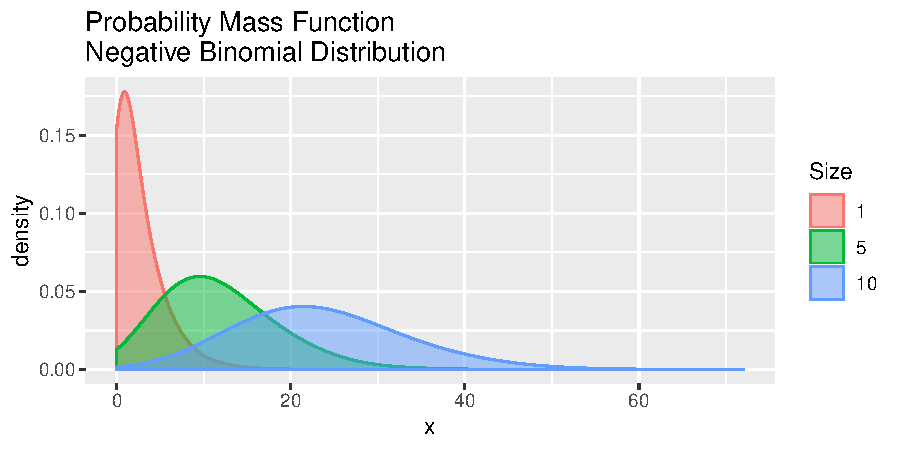
\includegraphics{Kor_BasicStats_files/figure-latex/unnamed-chunk-111-1} \end{center}

\hypertarget{f-uxbd84uxd3ec-f-distribution}{%
\subsection{F 분포 (F Distribution)}\label{f-uxbd84uxd3ec-f-distribution}}

\texttt{rf()}를 통해서 F 분포에서 무작위로 10,000개의 값을 서로 다른 자유도를 이용하여 추출하여 네 개의 벡터에 저장합니다. 이제는 아시겠지만 \texttt{rf()}의 \texttt{r}은 random을 의미합니다.

\begin{Shaded}
\begin{Highlighting}[]
\NormalTok{fa <-}\StringTok{ }\KeywordTok{rf}\NormalTok{(}\DataTypeTok{n =} \DecValTok{10000}\NormalTok{, }\DataTypeTok{df1 =} \DecValTok{1}\NormalTok{, }\DataTypeTok{df2 =} \DecValTok{50}\NormalTok{)}
\NormalTok{fb <-}\StringTok{ }\KeywordTok{rf}\NormalTok{(}\DataTypeTok{n =} \DecValTok{10000}\NormalTok{, }\DataTypeTok{df1 =} \DecValTok{5}\NormalTok{, }\DataTypeTok{df2 =} \DecValTok{100}\NormalTok{)}
\NormalTok{fc <-}\StringTok{ }\KeywordTok{rf}\NormalTok{(}\DataTypeTok{n =} \DecValTok{10000}\NormalTok{, }\DataTypeTok{df1 =} \DecValTok{50}\NormalTok{, }\DataTypeTok{df2 =} \DecValTok{50}\NormalTok{)}
\NormalTok{fd <-}\StringTok{ }\KeywordTok{rf}\NormalTok{(}\DataTypeTok{n =} \DecValTok{10000}\NormalTok{, }\DataTypeTok{df1 =} \DecValTok{50}\NormalTok{, }\DataTypeTok{df2 =} \DecValTok{500}\NormalTok{)}
\NormalTok{f <-}\StringTok{ }\KeywordTok{bind_rows}\NormalTok{(}\KeywordTok{tibble}\NormalTok{(}\DataTypeTok{x =}\NormalTok{ fa, }\DataTypeTok{DF1 =} \DecValTok{5}\NormalTok{, }\DataTypeTok{DF2 =} \DecValTok{5}\NormalTok{), }
               \KeywordTok{tibble}\NormalTok{(}\DataTypeTok{x =}\NormalTok{ fb, }\DataTypeTok{DF1 =} \DecValTok{5}\NormalTok{, }\DataTypeTok{DF2 =} \DecValTok{10}\NormalTok{), }
               \KeywordTok{tibble}\NormalTok{(}\DataTypeTok{x =}\NormalTok{ fc, }\DataTypeTok{DF1 =} \DecValTok{10}\NormalTok{, }\DataTypeTok{DF2 =} \DecValTok{5}\NormalTok{),}
               \KeywordTok{tibble}\NormalTok{(}\DataTypeTok{x =}\NormalTok{ fd, }\DataTypeTok{DF1 =} \DecValTok{10}\NormalTok{, }\DataTypeTok{DF2 =} \DecValTok{10}\NormalTok{))}
\end{Highlighting}
\end{Shaded}

이렇게 만들어진 데이터의 결과는 그림과 같습니다. 그리고 이제 \texttt{x} 값이 6보다 작거나 같은 경우로 하위 데이터를 만듭니다. 왜냐하면 굉장히 극단적인 수치들이 희소한 확률로 있기 때문에 그냥 그래프를 그리면 집단 별 차이를 보기가 조금 힘들 수도 있기 때문입니다. 그리고 전체 자유도를 지정해줄 것입니다. 자세한 내용은 나중에 \texttt{F-distribution}을 언급할 때 설명하도록 하겠습니다.

\begin{Shaded}
\begin{Highlighting}[]
\NormalTok{f <-}\StringTok{ }\KeywordTok{subset}\NormalTok{(f, x }\OperatorTok{<=}\StringTok{ }\DecValTok{6}\NormalTok{)}
\NormalTok{f}\OperatorTok{$}\NormalTok{DF <-}\StringTok{ }\NormalTok{f}\OperatorTok{$}\NormalTok{DF1 }\OperatorTok{*}\StringTok{ }\DecValTok{100} \OperatorTok{+}\StringTok{ }\NormalTok{f}\OperatorTok{$}\NormalTok{DF2}
\NormalTok{f}\OperatorTok{$}\NormalTok{DF <-}\StringTok{ }\KeywordTok{as.factor}\NormalTok{(f}\OperatorTok{$}\NormalTok{DF)}

\KeywordTok{ggplot}\NormalTok{(f, }\KeywordTok{aes}\NormalTok{(}\DataTypeTok{x =}\NormalTok{ x)) }\OperatorTok{+}
\StringTok{  }\KeywordTok{geom_density}\NormalTok{(}\KeywordTok{aes}\NormalTok{(}\DataTypeTok{color =}\NormalTok{ DF, }\DataTypeTok{fill =}\NormalTok{ DF), }\DataTypeTok{adjust =} \DecValTok{4}\NormalTok{, }\DataTypeTok{alpha =} \DecValTok{1}\OperatorTok{/}\DecValTok{2}\NormalTok{) }\OperatorTok{+}
\StringTok{  }\KeywordTok{guides}\NormalTok{(}\DataTypeTok{color=}\KeywordTok{guide_legend}\NormalTok{(}\DataTypeTok{title =} \StringTok{"DF1, DF2"}\NormalTok{)) }\OperatorTok{+}
\StringTok{  }\KeywordTok{guides}\NormalTok{(}\DataTypeTok{fill=}\KeywordTok{guide_legend}\NormalTok{(}\DataTypeTok{title =} \StringTok{"DF1, DF2"}\NormalTok{)) }\OperatorTok{+}
\StringTok{  }\KeywordTok{scale_color_discrete}\NormalTok{(}\DataTypeTok{labels =} \KeywordTok{c}\NormalTok{(}\StringTok{"1, 50"}\NormalTok{, }\StringTok{"5, 500"}\NormalTok{, }\StringTok{"50, 50"}\NormalTok{, }\StringTok{"50, 500"}\NormalTok{)) }\OperatorTok{+}
\StringTok{  }\KeywordTok{scale_fill_discrete}\NormalTok{(}\DataTypeTok{labels =} \KeywordTok{c}\NormalTok{(}\StringTok{"1, 50"}\NormalTok{, }\StringTok{"5, 500"}\NormalTok{, }\StringTok{"50, 50"}\NormalTok{, }\StringTok{"50, 500"}\NormalTok{)) }\OperatorTok{+}
\StringTok{  }\KeywordTok{ggtitle}\NormalTok{(}\StringTok{"Probability Density Function}\CharTok{\textbackslash{}n}\StringTok{F Distribution"}\NormalTok{)}
\end{Highlighting}
\end{Shaded}

\begin{center}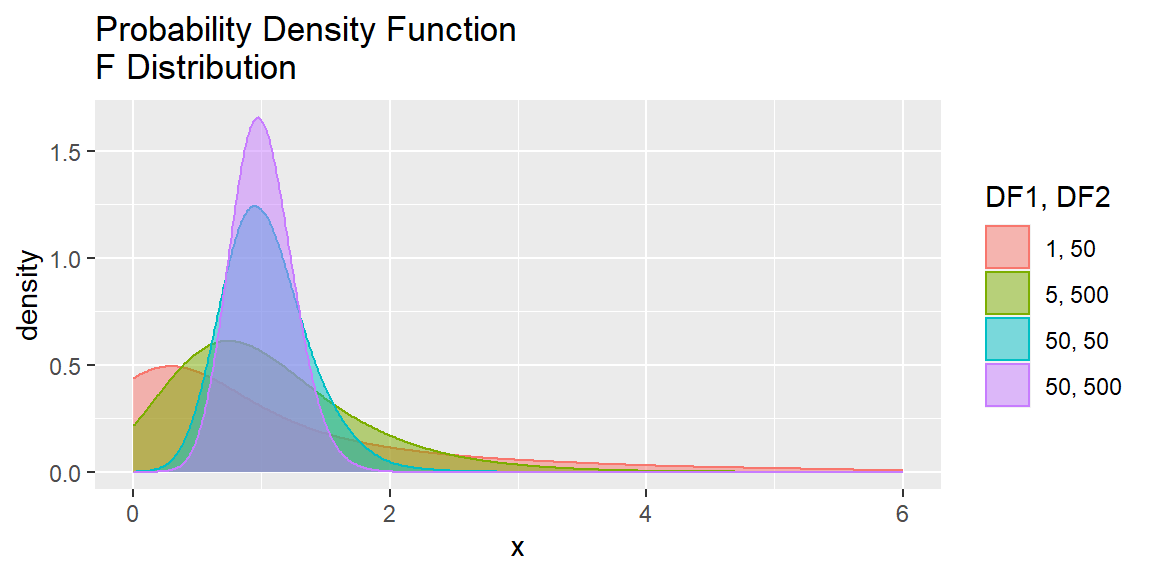
\includegraphics{Kor_BasicStats_files/figure-latex/unnamed-chunk-113-1} \end{center}

\texttt{DF1}이랑 \texttt{DF2}를 합쳐준다는 것은 F-분포의 특징 때문인데, 간단하게 말하자면 t-분포와 다르게 F-분포는 분자, 분모에 자유도가 하나씩 즉 2개가 필요하기 때문입니다.

오늘 포스팅한 내용 중에서는 처음 두 분포, 정규분포와 이항분포에 대해서는 숙지할 필요가 있고 나머지 분포들은 추후에 다시 다룰 기회가 있을 것이라고 생각합니다. 사실 분포는 엄청 많습니다: 웨이블, 토빗\ldots{} 뭐 여럿 있기 때문에 다 외우는 것은 어렵고 여기서는 단지 R-code로 구현하는 방법을 러프하게 살펴보았다고 할 수 있을 것입니다.

그리고 \texttt{ggplot()}은 손에 익도록 연습하는 것이 좋습니다. \textbf{R}의 장점 중 하나는 여타의 통계툴들에 비해 그래프 기능이 뛰어나다는 것입니다. \texttt{ggplot()}은 \textbf{R}이 그러한 명성을 얻게 해 준 공신 중 하나라고 할 수 있습니다.

\hypertarget{foundation-of-inference}{%
\chapter{Foundation of Inference}\label{foundation-of-inference}}

오늘 정리해볼 내용은 통계학의 핵심 중 하나인 추론(inference)의 근간이 되는 표본을 구하는 과정, 표집(sampling)을 어떻게 코딩으로 구현하는가와 관련된 것입니다. 즉, 이번 포스팅은 아래와 같은 내용을 주로 다룬다고 할 수 있습니다.

\begin{itemize}
\tightlist
\item
  R에서 표집 작업을 어떻게 수행하는가?
\item
  표집분포는 어떠한 형태를 띄는가?
\item
  표집분포를 어떻게 계산하는가?
\end{itemize}

이해를 돕기 위해서 사회과학 분야에서 널리 쓰는 세계발전지표(World Development Indicators, WDI)에서 변수들을 추출하여 활용해보도록 하겠습니다. 먼저 \texttt{WDI}를 라이브러리에서 로드해봅시다. 없으면 당연히 설치해야 겠죠?

\begin{Shaded}
\begin{Highlighting}[]
\CommentTok{# install.packages("WDI")}
\KeywordTok{library}\NormalTok{(WDI)}
\end{Highlighting}
\end{Shaded}

\texttt{WDI} 데이터셋에서 우리는 동일한 국가들이 시간을 거듭해(over time) 갖는 반복적인 값을 갖는 것을 확인할 수 있습니다. 이때 반복이란 동일하다는 얘기가 아니라 미국 2000년의 경제성장률, 미국 2001년의 경제성장률과 같은 식으로 일종의 패널(panel)을 이룬다는 것을 의미합니다.

이러한 자료의 구조는 자료 내에 내재할 수 있는 시간적 흐름의 상관효과, 그리고 동시기의 국가(단위)들 간에 존재할 수 있는 상관효과 등을 고려해주어야 함을 의미합니다. 물론, 여기서는 추론과 추론에 필요한 표집을 살펴볼 것이기 때문에 더 자세한 내용까지는 들어가지 않을 것입니다.

\texttt{WDI}에서 다음과 같은 변수들을 추출해 \texttt{WDI.data}라는 데이터프레임에 저장해보겠습니다.

\begin{itemize}
\tightlist
\item
  사망률 (mortality rate)
\item
  미국으로부터의 순 원조 유입 (net aid flows from US)
\item
  파상풍 예방주사 (newborns vaccinated for tetanus)
\item
  도시 지역 인구(전체 대비, urban pop \%)
\item
  무역개방성 (수출입 총합 대비 GDP, trade \% GDP)
\end{itemize}

\begin{Shaded}
\begin{Highlighting}[]
\NormalTok{WDI.data <-}\StringTok{  }
\StringTok{  }\KeywordTok{WDI}\NormalTok{(}\DataTypeTok{country =} \StringTok{"all"}\NormalTok{, }
      \DataTypeTok{indicator =} \KeywordTok{c}\NormalTok{(}\StringTok{"SH.DYN.NMRT"}\NormalTok{,}\StringTok{"DC.DAC.USAL.CD"}\NormalTok{, }\StringTok{"SH.VAC.TTNS.ZS"}\NormalTok{,}
                    \StringTok{"SP.URB.TOTL.IN.ZS"}\NormalTok{, }\StringTok{"NE.TRD.GNFS.ZS"}\NormalTok{), }
      \DataTypeTok{start =} \DecValTok{1990}\NormalTok{, }\DataTypeTok{end =} \DecValTok{2005}\NormalTok{, }\DataTypeTok{extra =} \OtherTok{FALSE}\NormalTok{, }\DataTypeTok{cache =} \OtherTok{NULL}\NormalTok{)}
\end{Highlighting}
\end{Shaded}

그리고 간단하게 자료에서 변수들의 형태를 살펴보겠습니다.

\begin{Shaded}
\begin{Highlighting}[]
\KeywordTok{par}\NormalTok{(}\DataTypeTok{mfrow =} \KeywordTok{c}\NormalTok{(}\DecValTok{1}\NormalTok{, }\DecValTok{3}\NormalTok{))}
\CommentTok{# 사망률}
\KeywordTok{hist}\NormalTok{(WDI.data}\OperatorTok{$}\NormalTok{SH.DYN.NMRT, }\DataTypeTok{main =} \StringTok{"Mortality rate"}\NormalTok{)}

\CommentTok{# 원조 (원조액은 두 가지: 첫 번째는 원자료로 두 번째는 로그화한 결과)}
\KeywordTok{hist}\NormalTok{(WDI.data}\OperatorTok{$}\NormalTok{DC.DAC.USAL.CD, }\DataTypeTok{main =} \StringTok{"Aid Raw"}\NormalTok{)}
\KeywordTok{hist}\NormalTok{(}\KeywordTok{log}\NormalTok{(WDI.data}\OperatorTok{$}\NormalTok{DC.DAC.USAL.CD}\FloatTok{+.1}\NormalTok{), }\DataTypeTok{main =} \StringTok{"Logged Aid"}\NormalTok{)}
\end{Highlighting}
\end{Shaded}

\begin{center}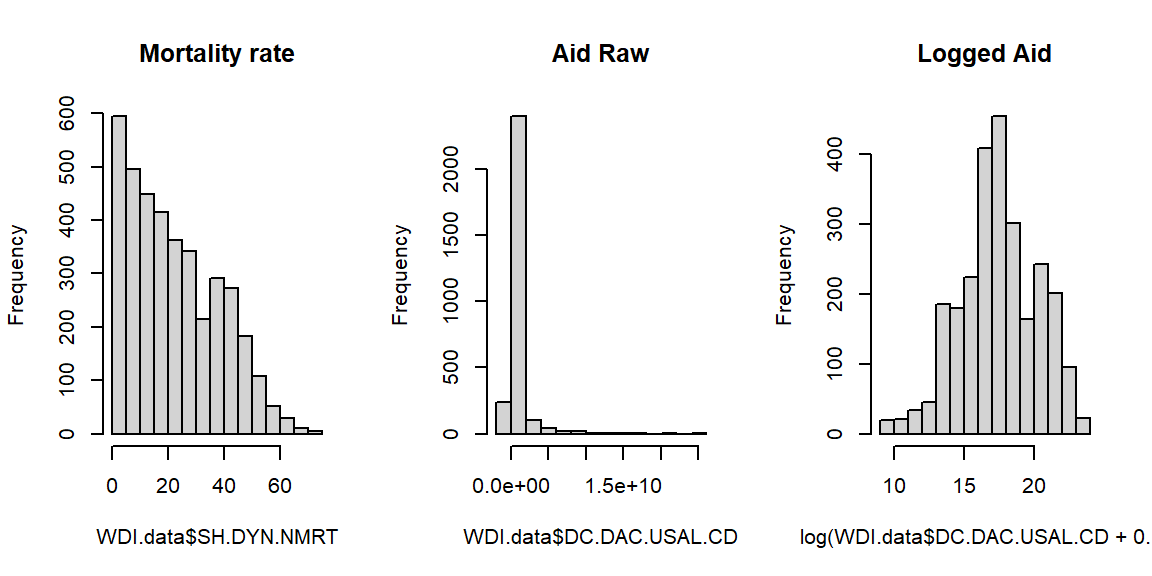
\includegraphics{Kor_BasicStats_files/figure-latex/unnamed-chunk-117-1} \end{center}

\begin{Shaded}
\begin{Highlighting}[]
\CommentTok{# 파상풍 예방주사}
\KeywordTok{hist}\NormalTok{(WDI.data}\OperatorTok{$}\NormalTok{SH.VAC.TTNS.ZS, }\DataTypeTok{main =} \StringTok{"Newborns vaccinated for tetanus"}\NormalTok{)}
\CommentTok{# 도시 인구}
\KeywordTok{hist}\NormalTok{(WDI.data}\OperatorTok{$}\NormalTok{SP.URB.TOTL.IN.ZS, }\DataTypeTok{main =} \StringTok{"Urban population rate"}\NormalTok{)}

\CommentTok{# 무역개방성 (마찬가지로 원조처럼 원자료와 로그화한 자료로)}
\KeywordTok{hist}\NormalTok{(WDI.data}\OperatorTok{$}\NormalTok{NE.TRD.GNFS.ZS, }\DataTypeTok{main =} \StringTok{"Trade openness_raw"}\NormalTok{)}
\end{Highlighting}
\end{Shaded}

\begin{center}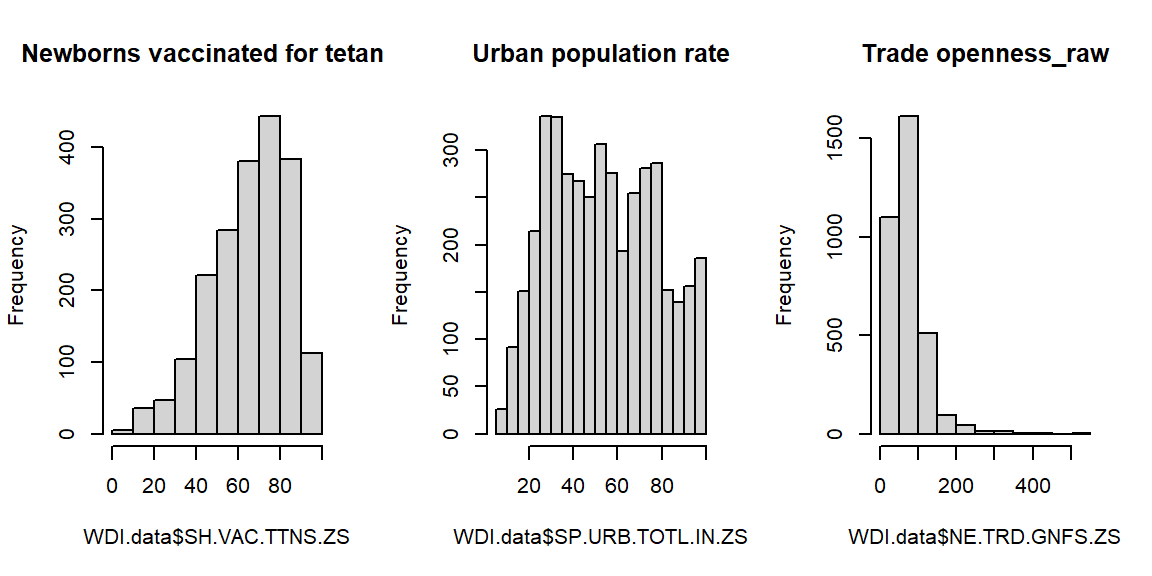
\includegraphics{Kor_BasicStats_files/figure-latex/unnamed-chunk-117-2} \end{center}

\begin{Shaded}
\begin{Highlighting}[]
\KeywordTok{hist}\NormalTok{(}\KeywordTok{log}\NormalTok{(WDI.data}\OperatorTok{$}\NormalTok{NE.TRD.GNFS.ZS), }\DataTypeTok{main =} \StringTok{"Logged trade openness"}\NormalTok{)}
\end{Highlighting}
\end{Shaded}

\begin{center}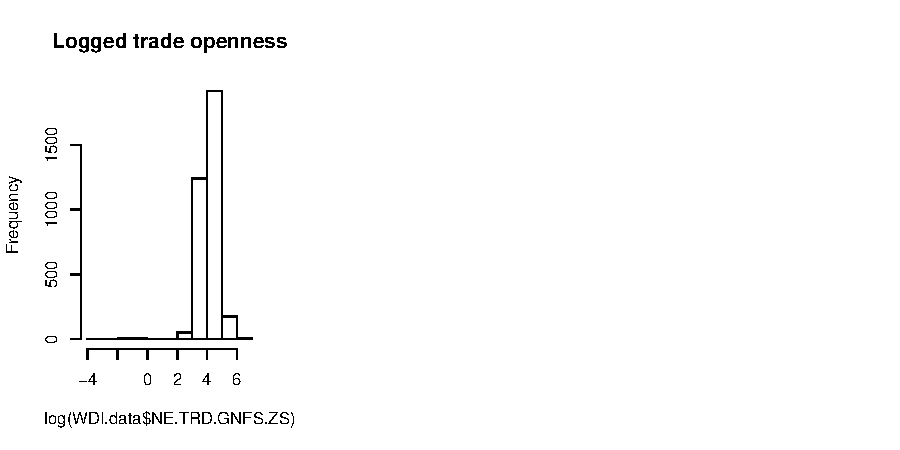
\includegraphics{Kor_BasicStats_files/figure-latex/unnamed-chunk-117-3} \end{center}

\hypertarget{uxd45cuxbcf8uxc744-uxd1b5uxd55c-uxbaa8uxc9d1uxb2e8-uxcd94uxb860-infer-population-using-samples}{%
\section{표본을 통한 모집단 추론 (Infer Population using Samples)}\label{uxd45cuxbcf8uxc744-uxd1b5uxd55c-uxbaa8uxc9d1uxb2e8-uxcd94uxb860-infer-population-using-samples}}

이제 이 변수들의 모집단을 우리가 모른다고 가정해보겠습니다. 대신 각각의 변수들로부터 50개의 관측치들을 무작위 표본을 취한다고 생각합시다. 그리고 우리는 이 무작위 표본을 5,000번 반복하여 뽑고 그렇게 뽑힌 5,000개의 무작위 표본들의 평균 분포를 그래프로 나타내겠습니다. 우선, 사망률에 대한 무작위 표본 1개를 뽑아보고, 그 표본 이름은 \texttt{samp1.mort} 라고 하자.

\begin{Shaded}
\begin{Highlighting}[]
\NormalTok{samp1.mort <-}\StringTok{ }\KeywordTok{sample}\NormalTok{(WDI.data}\OperatorTok{$}\NormalTok{SH.DYN.NMRT, }\DecValTok{50}\NormalTok{)}
\end{Highlighting}
\end{Shaded}

표본 평균과 모집단 평균을 비교해보겠습니다.

\begin{Shaded}
\begin{Highlighting}[]
\KeywordTok{mean}\NormalTok{(samp1.mort, }\DataTypeTok{na.rm =} \OtherTok{TRUE}\NormalTok{) }\CommentTok{# 사망률 표본의 평균}
\end{Highlighting}
\end{Shaded}

\begin{verbatim}
## [1] 23.83352
\end{verbatim}

\begin{Shaded}
\begin{Highlighting}[]
\CommentTok{## na.rm 옵션은 표본에 결측치가 있을 수 있을 때 중요하게 사용됩니다. }
\CommentTok{## 결측치 빼고 평균을 구하란 뜻입니다.}
\KeywordTok{mean}\NormalTok{(WDI.data}\OperatorTok{$}\NormalTok{SH.DYN.NMRT, }\DataTypeTok{na.rm =} \OtherTok{TRUE}\NormalTok{) }\CommentTok{# 사망률 모집단의 평균}
\end{Highlighting}
\end{Shaded}

\begin{verbatim}
## [1] 22.46436
\end{verbatim}

이제 5,000개의 표본들을 루프(loop)를 가지고 뽑아서 그 각각의 평균들을 벡터로 저장해보겠습니다. 이를 위해서 먼저 빈깡통, 빈 벡터(Blank vector)를 만들어야 합니다.

\begin{Shaded}
\begin{Highlighting}[]
\CommentTok{# 빈 벡터 만들기}
\NormalTok{sample_means50.mort <-}\StringTok{ }\KeywordTok{rep}\NormalTok{(}\OtherTok{NA}\NormalTok{, }\DecValTok{5000}\NormalTok{)}
\CommentTok{# 루프로 5,000개의 표본평균을 구해 저장하기}
\ControlFlowTok{for}\NormalTok{(i }\ControlFlowTok{in} \DecValTok{1}\OperatorTok{:}\DecValTok{5000}\NormalTok{) \{}
\NormalTok{  samp <-}\StringTok{ }\KeywordTok{sample}\NormalTok{(WDI.data}\OperatorTok{$}\NormalTok{SH.DYN.NMRT, }\DecValTok{50}\NormalTok{) }
\NormalTok{  sample_means50.mort[i] <-}\StringTok{ }\KeywordTok{mean}\NormalTok{(samp, }\DataTypeTok{na.rm =} \OtherTok{TRUE}\NormalTok{) }
\NormalTok{  \}}
\end{Highlighting}
\end{Shaded}

여기에서 루프의 의미는 원래 우리가 가지고 있던 \texttt{WDI}의 사망률 지표에서 50개씩 꺼낸 표본을 1개라고 할 때, 이와 같은 과정을 5,000번 반복하라는 것입니다. 그러면 5,000개의 표본을 얻게 되고, 이 중 당연히 결측치도 있을 수 있으므로 \texttt{na.rm()} 옵션으로 결측치를 제외하여 평균을 구하라고 코딩하는 것입니다.

평균을 구할 때, 요소 중에 \texttt{NA} (결측치)가 있으면 전체 평균 값도 \texttt{NA}로 계산되므로 이걸 처리해주어야 합니다. 자, 그럼 이렇게 구한 5,000개의 표본들의 평균들이 어떻게 분포되어 있는지 확인해보겠습니다. 히스토그램을 그려봅시다.: 50개의 값(values)을 가지는 5,000개의 표본평균 각각의 평균들의 분포를 플롯으로 살펴보는 것입니다.

먼저 1개의 표본평균과 모집단 평균을 비교했을 때랑 보자면, 5,000개의 표본평균들과 모집단 평균 간의 차이가 현격하게 감소한 것을 확인할 수 있습니다. 이 시뮬레이션에서 우리는 직관적으로 한 가지를 확인할 수 있습니다. 무작위라는 조건 하에서 표집을 반복할 때, 그 평균들의 평균은 모집단의 평균으로 수렴하므로 우리는 이와 같은 작업을 통해 실제로 모집단을 모르는 상황에서 표본들로 모집단의 특성을 추론할 수 있다는 것입니다.

\begin{Shaded}
\begin{Highlighting}[]
\KeywordTok{mean}\NormalTok{(sample_means50.mort, }\DataTypeTok{na.rm =} \OtherTok{TRUE}\NormalTok{)}
\end{Highlighting}
\end{Shaded}

\begin{verbatim}
## [1] 22.42464
\end{verbatim}

\begin{Shaded}
\begin{Highlighting}[]
\KeywordTok{mean}\NormalTok{(WDI.data}\OperatorTok{$}\NormalTok{SH.DYN.NMRT, }\DataTypeTok{na.rm =} \OtherTok{TRUE}\NormalTok{)}
\end{Highlighting}
\end{Shaded}

\begin{verbatim}
## [1] 22.46436
\end{verbatim}

이제 전체 인구 대비 도시 인구의 비율 변수를 살펴보겠습니다. 주어진 중심극한정리 (Central Limit Theorem)에 따라 우리는 오직 1개의 표본만을 취해 모집단에 대한 95\%의 신뢰 구간을 계산해볼 것입니다. 이전과 마찬가지로 50개의 값을 무작위로 추출해 \texttt{samp.pop} 이라는 자료에 담고 이 표본을 이용하여 평균과 표준오차를 계산해보겠습니다.

\begin{Shaded}
\begin{Highlighting}[]
\NormalTok{samp.pop <-}\StringTok{ }\KeywordTok{sample}\NormalTok{(WDI.data}\OperatorTok{$}\NormalTok{SP.URB.TOTL.IN.ZS, }\DecValTok{50}\NormalTok{)}
\NormalTok{mean.pop <-}\StringTok{ }\KeywordTok{mean}\NormalTok{(samp.pop, }\DataTypeTok{na.rm =} \OtherTok{TRUE}\NormalTok{) }\CommentTok{# 표본의 평균}
\NormalTok{se.pop <-}\StringTok{ }\KeywordTok{sd}\NormalTok{(samp.pop, }\DataTypeTok{na.rm =} \OtherTok{TRUE}\NormalTok{)}\OperatorTok{/}\KeywordTok{sqrt}\NormalTok{(}\KeywordTok{length}\NormalTok{(samp.pop)) }\CommentTok{# 표준오차}

\CommentTok{# 평균을 중심으로 95%의 신뢰구간을 구해보자 (위/아래)}
\NormalTok{lower.pop <-}\StringTok{ }\NormalTok{mean.pop }\OperatorTok{-}\StringTok{ }\NormalTok{(}\FloatTok{1.96} \OperatorTok{*}\StringTok{ }\NormalTok{se.pop)}
\NormalTok{upper.pop <-}\StringTok{ }\NormalTok{mean.pop }\OperatorTok{+}\StringTok{ }\NormalTok{(}\FloatTok{1.96} \OperatorTok{*}\StringTok{ }\NormalTok{se.pop)}

\CommentTok{# 95% 신뢰 구간의 경계 값과 평균을 리스트 자료 유형으로 저장한다.}
\KeywordTok{c}\NormalTok{(lower.pop, mean.pop, upper.pop)}
\end{Highlighting}
\end{Shaded}

\begin{verbatim}
## [1] 46.77348 52.72559 58.67770
\end{verbatim}

\begin{Shaded}
\begin{Highlighting}[]
\CommentTok{# 평균 추정치와 신뢰구간을 그래프로 만들 수 있다.}
\KeywordTok{library}\NormalTok{(tidyverse)}
\NormalTok{estimates.df <-}\StringTok{ }\KeywordTok{bind_rows}\NormalTok{(}\KeywordTok{tibble}\NormalTok{(lower.pop, mean.pop, upper.pop))}
\NormalTok{estimates.df}\OperatorTok{$}\NormalTok{sample.no <-}\StringTok{ }\DecValTok{1}
\KeywordTok{library}\NormalTok{(ggplot2)}
\KeywordTok{ggplot}\NormalTok{(}\DataTypeTok{data =}\NormalTok{ estimates.df, }\KeywordTok{aes}\NormalTok{(}\DataTypeTok{x =}\NormalTok{ sample.no)) }\OperatorTok{+}
\StringTok{  }\KeywordTok{geom_pointrange}\NormalTok{(}\KeywordTok{aes}\NormalTok{(}\DataTypeTok{y =}\NormalTok{ mean.pop, }\DataTypeTok{ymin =}\NormalTok{ lower.pop, }\DataTypeTok{ymax =}\NormalTok{ upper.pop))}
\end{Highlighting}
\end{Shaded}

\begin{center}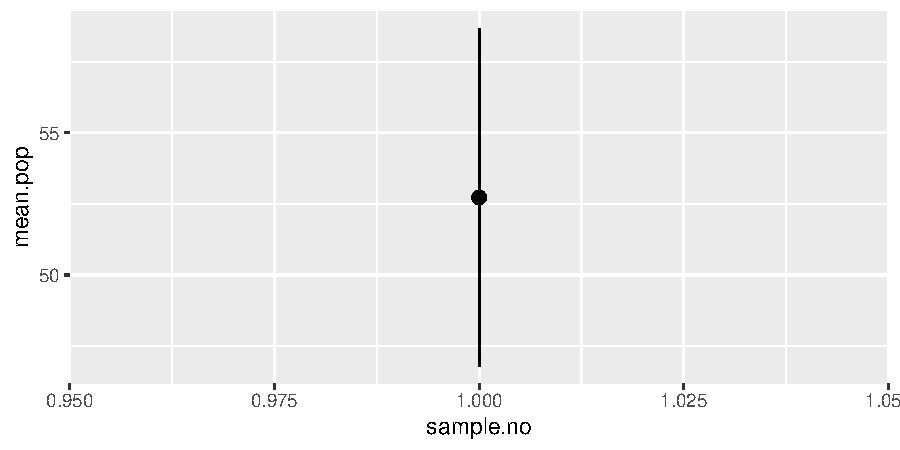
\includegraphics{Kor_BasicStats_files/figure-latex/unnamed-chunk-122-1} \end{center}

표본 1개의 평균값과 95\% 신뢰구간의 경계값 (bound)을 표현한 그래프입니다.

동일한 작업을 루프를 이용하여 20개의 표본을 대상으로 하는 평균과 95\% 신뢰구간의 하위/상위 경계값을 구해보겠습니다.

\begin{Shaded}
\begin{Highlighting}[]
\NormalTok{mean.pop}\FloatTok{.20}\NormalTok{ <-}\StringTok{ }\KeywordTok{rep}\NormalTok{(}\OtherTok{NA}\NormalTok{, }\DecValTok{20}\NormalTok{)}
\NormalTok{lower.pop}\FloatTok{.20}\NormalTok{ <-}\StringTok{ }\KeywordTok{rep}\NormalTok{(}\OtherTok{NA}\NormalTok{, }\DecValTok{20}\NormalTok{)}
\NormalTok{upper.pop}\FloatTok{.20}\NormalTok{ <-}\StringTok{ }\KeywordTok{rep}\NormalTok{(}\OtherTok{NA}\NormalTok{, }\DecValTok{20}\NormalTok{)}

\ControlFlowTok{for}\NormalTok{(x }\ControlFlowTok{in} \DecValTok{1}\OperatorTok{:}\DecValTok{20}\NormalTok{) \{}
\NormalTok{  samp.pop <-}\StringTok{ }\KeywordTok{sample}\NormalTok{(WDI.data}\OperatorTok{$}\NormalTok{SP.URB.TOTL.IN.ZS, }\DecValTok{50}\NormalTok{)}
\NormalTok{  mean.pop}\FloatTok{.20}\NormalTok{[x] <-}\StringTok{ }\KeywordTok{mean}\NormalTok{(samp.pop, }\DataTypeTok{na.rm =} \OtherTok{TRUE}\NormalTok{)}
\NormalTok{  lower.pop}\FloatTok{.20}\NormalTok{[x] <-}\StringTok{ }\NormalTok{mean.pop}\FloatTok{.20}\NormalTok{[x] }\OperatorTok{-}\StringTok{ }
\StringTok{    }\NormalTok{(}\FloatTok{1.96} \OperatorTok{*}\StringTok{ }\NormalTok{(}\KeywordTok{sd}\NormalTok{(samp.pop, }\DataTypeTok{na.rm =} \OtherTok{TRUE}\NormalTok{)}\OperatorTok{/}\KeywordTok{sqrt}\NormalTok{(}\KeywordTok{length}\NormalTok{(samp.pop))))}
\NormalTok{  upper.pop}\FloatTok{.20}\NormalTok{[x] <-}\StringTok{ }\NormalTok{mean.pop}\FloatTok{.20}\NormalTok{[x] }\OperatorTok{+}\StringTok{ }
\StringTok{    }\NormalTok{(}\FloatTok{1.96} \OperatorTok{*}\StringTok{ }\NormalTok{(}\KeywordTok{sd}\NormalTok{(samp.pop, }\DataTypeTok{na.rm =} \OtherTok{TRUE}\NormalTok{)}\OperatorTok{/}\KeywordTok{sqrt}\NormalTok{(}\KeywordTok{length}\NormalTok{(samp.pop))))}
\NormalTok{\}}
\end{Highlighting}
\end{Shaded}

이렇게 구한 총 20개의 표본평균, 하위경계값, 상위경계값을 \texttt{estimates.df.20}이라는 데이터프레임에 저장하고 그래프로 나타내보겠습니다.

\begin{Shaded}
\begin{Highlighting}[]
\NormalTok{estimates.df}\FloatTok{.20}\NormalTok{ <-}\StringTok{ }\KeywordTok{tibble}\NormalTok{(lower.pop}\FloatTok{.20}\NormalTok{, mean.pop}\FloatTok{.20}\NormalTok{,upper.pop}\FloatTok{.20}\NormalTok{)}
\NormalTok{estimates.df}\FloatTok{.20}\OperatorTok{$}\NormalTok{sample.no <-}\StringTok{ }\KeywordTok{c}\NormalTok{(}\DecValTok{1}\OperatorTok{:}\DecValTok{20}\NormalTok{)}
\KeywordTok{ggplot}\NormalTok{(}\DataTypeTok{data =}\NormalTok{ estimates.df}\FloatTok{.20}\NormalTok{, }\KeywordTok{aes}\NormalTok{(}\DataTypeTok{x =}\NormalTok{ sample.no)) }\OperatorTok{+}
\StringTok{  }\KeywordTok{geom_pointrange}\NormalTok{(}\KeywordTok{aes}\NormalTok{(}\DataTypeTok{y =}\NormalTok{ mean.pop}\FloatTok{.20}\NormalTok{, }
                      \DataTypeTok{ymin =}\NormalTok{ lower.pop}\FloatTok{.20}\NormalTok{, }
                      \DataTypeTok{ymax =}\NormalTok{ upper.pop}\FloatTok{.20}\NormalTok{))}
\end{Highlighting}
\end{Shaded}

\begin{center}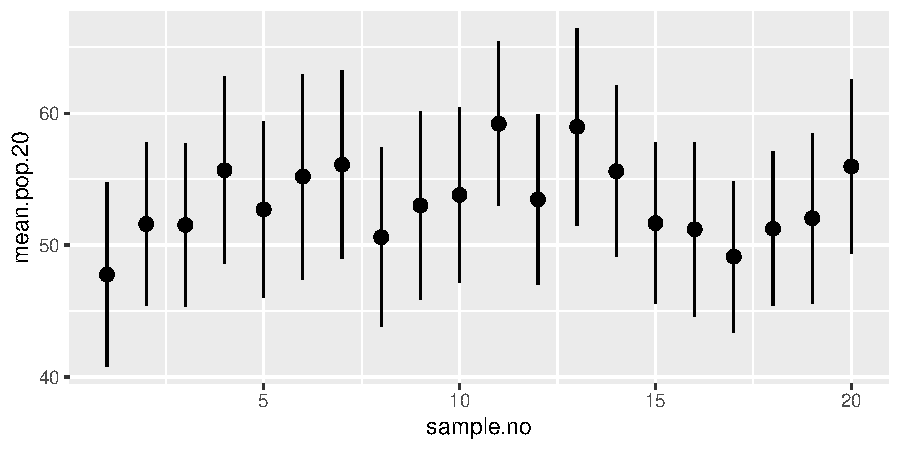
\includegraphics{Kor_BasicStats_files/figure-latex/unnamed-chunk-124-1} \end{center}

사실 위와 같은 형태의 그래프를 제공하는 함수가 \texttt{coefplot()}이라고 따로 존재합니다. 요즘에는 회귀분석의 결과표만 보여주기 보다는 평균과 신뢰구간을 같이 보여줄 수 있는 회귀계수 그래프를 위와 같이 제시하는 추세입니다.

\begin{Shaded}
\begin{Highlighting}[]
\KeywordTok{ggplot}\NormalTok{(}\DataTypeTok{data =}\NormalTok{ estimates.df}\FloatTok{.20}\NormalTok{, }\KeywordTok{aes}\NormalTok{(}\DataTypeTok{x =}\NormalTok{ sample.no)) }\OperatorTok{+}
\StringTok{  }\KeywordTok{geom_pointrange}\NormalTok{(}\KeywordTok{aes}\NormalTok{(}\DataTypeTok{y =}\NormalTok{ mean.pop}\FloatTok{.20}\NormalTok{, }
                      \DataTypeTok{ymin =}\NormalTok{ lower.pop}\FloatTok{.20}\NormalTok{, }\DataTypeTok{ymax =}\NormalTok{ upper.pop}\FloatTok{.20}\NormalTok{)) }\OperatorTok{+}\StringTok{ }
\StringTok{  }\KeywordTok{geom_hline}\NormalTok{(}\DataTypeTok{data =}\NormalTok{ WDI.data, }
             \KeywordTok{aes}\NormalTok{(}\DataTypeTok{yintercept =} \KeywordTok{mean}\NormalTok{(SP.URB.TOTL.IN.ZS, }\DataTypeTok{na.rm =} \OtherTok{TRUE}\NormalTok{))) }\OperatorTok{+}\StringTok{ }
\StringTok{  }\KeywordTok{coord_flip}\NormalTok{() }\OperatorTok{+}\StringTok{ }
\StringTok{  }\KeywordTok{theme_bw}\NormalTok{() }\OperatorTok{+}\StringTok{ }
\StringTok{  }\KeywordTok{xlab}\NormalTok{(}\StringTok{"Sample number"}\NormalTok{) }\OperatorTok{+}\StringTok{ }\KeywordTok{ylab}\NormalTok{(}\StringTok{"Estimates"}\NormalTok{) }\OperatorTok{+}\StringTok{ }
\StringTok{  }\KeywordTok{ggtitle}\NormalTok{(}\StringTok{"Sample means for urban pop, with 95% confidence intervals"}\NormalTok{)}
\end{Highlighting}
\end{Shaded}

\begin{center}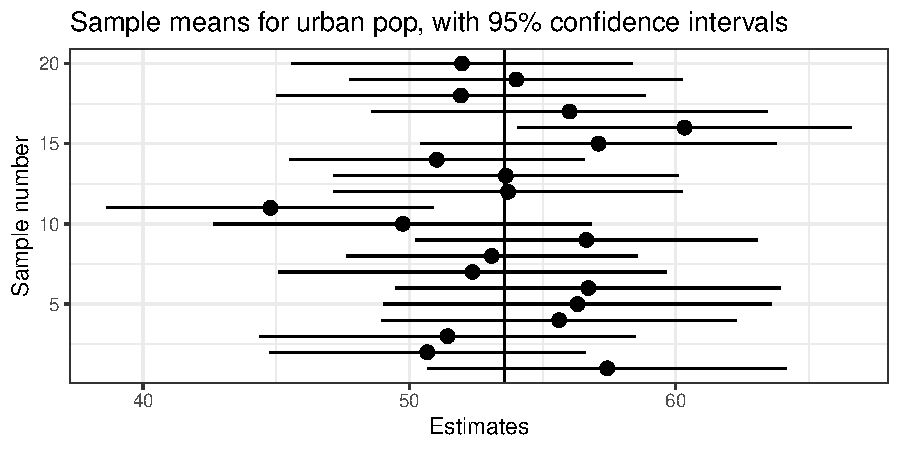
\includegraphics{Kor_BasicStats_files/figure-latex/unnamed-chunk-125-1} \end{center}

몇 가지 추가적인 특징들을 더 보여주기 위하여 한 가지 과정을 더해보았습니다. 먼저 95\% 신뢰구간 밖에 존재하는 값들을 이탈치 (outliers)라고 할 때, 그 이탈치를 의미하는 더미변수를 하나 만들어보겠습니다. 이탈치면 1, 이탈치가 아니면 0의 값을 갖는 변수를 만들겠다는 것입니다. 95\% 신뢰구간을 벗어났다는 것은 표본평균을 가지고 추론한 구간추정 범위 내에 모집단 평균이 존재하지 않는다는 것입니다.

\begin{Shaded}
\begin{Highlighting}[]
\NormalTok{estimates.df}\FloatTok{.20}\OperatorTok{$}\NormalTok{outside <-}\StringTok{ }
\StringTok{  }\KeywordTok{ifelse}\NormalTok{(estimates.df}\FloatTok{.20}\OperatorTok{$}\NormalTok{lower.pop}\FloatTok{.20} \OperatorTok{>}\StringTok{ }
\StringTok{           }\KeywordTok{mean}\NormalTok{(WDI.data}\OperatorTok{$}\NormalTok{SP.URB.TOTL.IN.ZS, }\DataTypeTok{na.rm =} \OtherTok{TRUE}\NormalTok{) }\OperatorTok{|}\StringTok{ }
\StringTok{           }\NormalTok{estimates.df}\FloatTok{.20}\OperatorTok{$}\NormalTok{upper.pop}\FloatTok{.20} \OperatorTok{<}\StringTok{ }
\StringTok{           }\KeywordTok{mean}\NormalTok{(WDI.data}\OperatorTok{$}\NormalTok{SP.URB.TOTL.IN.ZS, }\DataTypeTok{na.rm =} \OtherTok{TRUE}\NormalTok{), }\DecValTok{1}\NormalTok{, }\DecValTok{0}\NormalTok{)}
\end{Highlighting}
\end{Shaded}

마지막으로 표본평균 + 95\% 신뢰구간이 모집단 평균을 포함하지 않는 경우에는 그래프 라인의 색을 빨간 색으로 바꾸는 코딩을 짜보겠습니다.

\begin{Shaded}
\begin{Highlighting}[]
\KeywordTok{ggplot}\NormalTok{(}\DataTypeTok{data =}\NormalTok{ estimates.df}\FloatTok{.20}\NormalTok{, }
       \KeywordTok{aes}\NormalTok{(}\DataTypeTok{x =}\NormalTok{ sample.no, }\DataTypeTok{color =} \KeywordTok{as.factor}\NormalTok{(outside))) }\OperatorTok{+}
\StringTok{  }\KeywordTok{geom_pointrange}\NormalTok{(}\KeywordTok{aes}\NormalTok{(}\DataTypeTok{y =}\NormalTok{ mean.pop}\FloatTok{.20}\NormalTok{, }
                      \DataTypeTok{ymin =}\NormalTok{ lower.pop}\FloatTok{.20}\NormalTok{, }
                      \DataTypeTok{ymax =}\NormalTok{ upper.pop}\FloatTok{.20}\NormalTok{)) }\OperatorTok{+}\StringTok{ }
\StringTok{  }\KeywordTok{geom_hline}\NormalTok{(}\DataTypeTok{data =}\NormalTok{ WDI.data, }
             \KeywordTok{aes}\NormalTok{(}\DataTypeTok{yintercept =} \KeywordTok{mean}\NormalTok{(SP.URB.TOTL.IN.ZS, }\DataTypeTok{na.rm =} \OtherTok{TRUE}\NormalTok{))) }\OperatorTok{+}\StringTok{ }
\StringTok{  }\KeywordTok{coord_flip}\NormalTok{() }\OperatorTok{+}\StringTok{ }
\StringTok{  }\KeywordTok{theme_bw}\NormalTok{() }\OperatorTok{+}\StringTok{ }
\StringTok{  }\KeywordTok{scale_color_manual}\NormalTok{(}\DataTypeTok{name =} \StringTok{""}\NormalTok{, }\DataTypeTok{values=}\KeywordTok{c}\NormalTok{(}\StringTok{"#9999CC"}\NormalTok{, }\StringTok{"#CC6666"}\NormalTok{)) }\OperatorTok{+}
\StringTok{  }\KeywordTok{theme}\NormalTok{(}\DataTypeTok{legend.position=}\StringTok{"none"}\NormalTok{) }\OperatorTok{+}
\StringTok{  }\KeywordTok{xlab}\NormalTok{(}\StringTok{"Sample number"}\NormalTok{) }\OperatorTok{+}\StringTok{ }\KeywordTok{ylab}\NormalTok{(}\StringTok{"Estimates"}\NormalTok{) }\OperatorTok{+}\StringTok{ }
\StringTok{  }\KeywordTok{ggtitle}\NormalTok{(}\StringTok{"Sample means for urban pop, with 95% confidence intervals"}\NormalTok{)}
\end{Highlighting}
\end{Shaded}

\begin{center}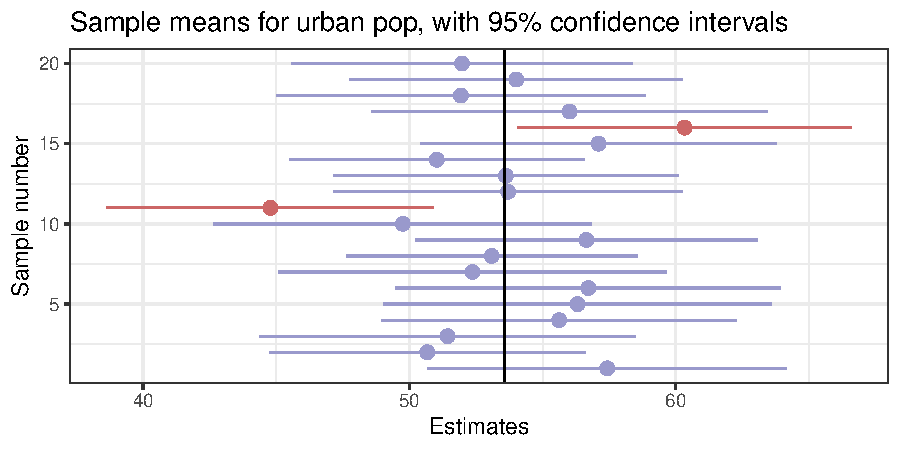
\includegraphics{Kor_BasicStats_files/figure-latex/unnamed-chunk-127-1} \end{center}

실선이 도시 인구 비율의 모집단 평균이라고 할 때, 총 4개의 표본이 평균과 그 평균을 중심으로 한 표준오차 (95\% 신뢰구간) 내에 모집단 평균을 포함하지 않는 것을 확인할 수 있습니다.

\hypertarget{uxd3c9uxade0uxc758-uxcc28uxc774difference-of-means-uxadf8uxb9acuxace0-uxbd84uxc0b0uxbd84uxc11danalysis-of-variance-anova}{%
\section{평균의 차이(difference of means), 그리고 분산분석(analysis of variance, ANOVA)}\label{uxd3c9uxade0uxc758-uxcc28uxc774difference-of-means-uxadf8uxb9acuxace0-uxbd84uxc0b0uxbd84uxc11danalysis-of-variance-anova}}

사회과학, 정량적 사회과학 연구가 추구하는 목적 중 하나는 인과관계에 관한 추론, 인과추론(causal inference)입니다. 인과관계란 어떤 현상의 생성경로를 추적하기 위한 분석구도로서 경험적으로 확증될 수 없는 논리적 관계를 의미합니다.

인과관계의 성격은 유리스틱에 따라 달리 규정되지만, 생산(producing)의 관계라는 측면에서는 견해가 일치합니다. 즉, 원인이 기능하여 결과를 생산한다는 것이죠.

\begin{itemize}
\tightlist
\item
  인과관계는 감각경험을 통해 인지할 수 있는 상호독립적 단위로 구성되며, 원인과 결과는
  서로 다른 현상으로 일정한 기능적 연관성 이외에 어떠한 본질적 동질성도 공유하지 않는다고 봅니다.
\item
  또한 경험과학적 시각에서 모든 현상의 원인과 결과 사이의 인과관계는 규칙성과 재생성을
  나타냅니다.
\item
  이 규칙성은 잠정적인 것으로 간주되는데, 그 이유는 네 가지 맥락에서 비롯됩니다.
\end{itemize}

\begin{enumerate}
\def\labelenumi{\arabic{enumi}.}
\tightlist
\item
  어떤 사회현상의 인과적 생성경로는 귀납적으로 추론되나, 귀납적 일반화는 귀납사례의
  범주에 제한되어 조건적입니다.
\item
  마찬가지로 밝혀진 원인들은 충분조건 또는 필요조건에 불과합니다.
\item
  우리는 인과관계를 경험적으로 확인할 수는 없습니다.
\item
  인간의 상호작용으로 나타나는 사회현상은 가변적이므로 그들 간 인과관계도 유동적입니다.
\end{enumerate}

우리는 \texttt{X}와 \texttt{Y}의 관계를 논리적으로 설정할 수 있을 때, \texttt{X}를 원인으로, \texttt{Y}를 결과로 받아들여 양자 간 인과관계를 부여합니다.

\begin{itemize}
\tightlist
\item
  단, 경험과학적 사회과학연구에서는 도출된 인과관계를 일단의 가정과 선행조건이 충족되었을 경우에 한해 성립되는 개연적 관계로 받아들입니다.
\item
  즉, 인과관계는 언제든 변할 수 있는 경향이나 추세라는 것입니다.
\end{itemize}

인과추론에 요구되는 근거는 크게 세 가지로 구분할 수 있습니다. 첫째 시간적 순차, 둘째 항상적 연계, 셋째, 탈허위성입니다.

\begin{enumerate}
\def\labelenumi{\arabic{enumi}.}
\tightlist
\item
  시간적 순차(time-order)
\end{enumerate}

\begin{itemize}
\tightlist
\item
  원인은 반드시 결과에 시간적으로 앞서야 합니다.
\item
  시간차(time lag)의 경험적 근거가 필요하다.
\end{itemize}

\begin{enumerate}
\def\labelenumi{\arabic{enumi}.}
\setcounter{enumi}{1}
\tightlist
\item
  항상적 연계
\end{enumerate}

\begin{itemize}
\tightlist
\item
  어떤 현상(원인)의 변화가 다른 현상(결과)의 규칙적 변화를 지속적\(\cdot\)안정적으로
  수반할 때, 이들 사이의 인과관계를 추론할 수 있습니다.
\item
  실제 연구과정에 있어서 항상적 연계라는 논리적 척도는 통계적 공변(statistical covariance), 함수적 상관관계(functional correlation)라는 경험적 척도로 대체됩니다.
\item
  예측변수와 종속변수 간의 공변규칙성이 연구의 시간적\(\cdot\)공간적 선행조건 하에서
  안정적으로 나타날 때, 인과추론에 요구되는 경험적 근거를 얻을 수 있습니다.
\item
  그러나 공변규칙성만으로 인과관계의 존재를 단정해서는 안 됩니다(관계는 경험적 관측 불가).
\item
  단 항상적 연계는 인과관계의 필요조건입니다(항상적 연계 없으면 일단 인과관계도 없습니다).
\end{itemize}

\begin{enumerate}
\def\labelenumi{\arabic{enumi}.}
\setcounter{enumi}{2}
\tightlist
\item
  탈허위성
\end{enumerate}

\begin{itemize}
\tightlist
\item
  인과관계가 허위성을 가지지 않고 진정한(genuine) 것이어야 한다는 뜻입니다.
\end{itemize}

\hypertarget{uxd3c9uxade0-uxcc28uxc774uxb97c-uxbcf4uxb294-uxc774uxc720}{%
\subsection{평균 차이를 보는 이유}\label{uxd3c9uxade0-uxcc28uxc774uxb97c-uxbcf4uxb294-uxc774uxc720}}

앞에서 표집을 했을 때와 유사합니다. 사실 우리가 관측한 사회현상이 모집단 그 자체의 사회현상이라고 `결코' 단언할 수 없습니다. 인과성(causality)에 대한 문제는, ``어떠한 현상에 대한 원인은 무엇인가?''에 답을 하기 위함입니다. 이것이야말로 사회과학에서 가장 핵심이
라고 할 수 있습니다. 과학의 정수 는 이론의 수립이며, 이론은 인과적 진술이기 때문입니다. 현상에서 보이지 않는 법칙을 발견하고, 다듬어 나가는 것이 우리 사회``과학자''들이 하는 일이라고 할 수 있습니다. 때문에 인과성(causality)은 우리의 핵심 주제일 수밖에 없습니다.

인과효과(causal effect)는 다른 요인들이 통제되었을 때, 주요 변인들이 만들어내는 결과의 차이-영향이라고 할 수 있습니다. 예를 들어, 프랑스 혁명의 인과적 효과는 프랑스 혁명이 일어나지 않았을 때의 결과와 비교해볼 때 확인할 수 있습니다. 그런데 문제는 원인이 있을 때와 없을 때를 사회과학에서는 동시에 관찰할 수가 없다는 것입니다(반사실적 사례의 관측불가능성).

이 문제가 바로 인과추론의 근본적 문제입니다. 이 문제를 해결하기 위해 우리는 두 가지 가설적 방법들을 사용하게 됩니다. 사례를 들어보겠습니다. 가설로 ``재직 중인 사람이 선거에서 득표율이 높을 것이다.''라고 할 때, 종속변인은 민주당원이 갖는 득표율이며, 이를 예측하기 위한 변인은 재직 여부가 될 것입니다. 그래서 재직 중인 사람이 나갔을 때 득표율과 새롭게 나간 사람의 득표율
을 비교, 그 사이의 차이가 바로 인과 효과라고 할 수 있을 것입니다. 예측변인을 제외 한 나머지는 통제되어야 합니다---즉, 변하지 않도록 해야 한다는 것(holding constant)입니다. 이러한 통제의 대상을 어떻게 선정할 것인가는 연구를 설계하는 연구자의 역량에 따라 좌우됩니다.

위 사례에서 반사실적 조건문(counterfactuals)을 통해 우리가 얻어낼 수 있는 것이 실현된 인과 효과(realized causal effect)이다. 사회과학 연구방법론에 있어서 교과서적으로 읽히는 King, Keohane, 그리고 Verba의 1994년 저작 ``Designing Social Inquiry'', 이하 KKV는 이 문제에 대해 우리는 관측가능한 효과에서 체계적인 것과 비체계적인 것을 구분해야 한다고 강조합니다.\footnote{King, Gary, Robert Keohane, and Sidney Verba. 1994. \emph{Designing Social Inquiry}. Princeton: Princeton University Press.} KKV는 우리가 체계적인 변화에 주목해야 한다고 주장합니다. 그리고 그것을 위해서 우리는 가설적인 반복을 통해 비체계적 요인들을 상쇄시키고, 체계적인 요인들만의 영향---평균적인 인과 효과를 살펴볼 수 있다는 것입니다.

사실, 우리는 우리가 관찰하는 대상 안에 오차(error)가 존재한다고 생각할 수밖에 없기 때문에, 그것을 최소화시키는(maximizing error term) 것이야말로 체계적인 변화의 요인을 추적할 수 있는 방법이 될 수 있습니다. 가설적 반복을 통해 나오는 하나의 분석단위에 대한 확률적인 인과 효과를 평균적으로 보는 것(Random Causal Effect for \(\text{unit}_i\)), 즉 평균적 인과 효과(Mean causal effect)는 체계적인 요인들이 가지고 오는 영향의 평균을 의미합니다. KKV는 이와 같이 관측된 인과 효과에서 체계적-비체계적 효과를 구분하는 것을 포함하여 인과 효과의 논의를 발전시켰습니다.

여기서 하나 더 살펴보아야 하는 것이 바로 분산입니다. 분산이란 실제로 관측된 데이터들이 평균에서 어느 정도 수준으로 흩어져 있는지를 보여주는 통계치입니다. 즉, 관측된 사회현상은 필연적으로 일정한 수준의 분산을 가지게 되는데, 이 변수 자체 분산을 고려하여, 우리가 보고자 하는 두 변수의 관계에 적용할 수 있습니다. 간단히 정리하자면, 두 변수의 평균의 차이가 두 변수의 분산 정도를 무시할 수 있을 정도로 명확하다면, 우리는 통계적으로 이 두 변수 간의 차이가 유의미하다고 볼 수 있습니다. 이에 관한 내용은 추후에 더 자세히 살펴볼 기회가 있을 것입니다.

일단 여기까지가 바로 우리가 인과추론을 이해하기 위한 기초로서 평균 차 분석의 논리를 살펴보아야 하는 이유입니다. 이론적 논의는 여기까지하고, \textbf{R}을 통해 실제 자료를 바탕으로 예제를 통해 구체적인 논의를 이끌어 나가보도록 하겠습니다. 오픈소스로 공개되어 있는 정부의 질(Quality of Government, 이햐 QoG) 데이터셋의 교차사례 자료(cross-section data)를 사용해보겠습니다.

\begin{Shaded}
\begin{Highlighting}[]
\KeywordTok{library}\NormalTok{(ezpickr)}
\NormalTok{QOG <-}\StringTok{ }\KeywordTok{pick}\NormalTok{(}\DataTypeTok{file =} \StringTok{"http://www.qogdata.pol.gu.se/data/qog_bas_ts_jan19.dta"}\NormalTok{)}
\CommentTok{# 2010년도 자료만 보겠습니다.}
\NormalTok{QOG <-}\StringTok{ }\NormalTok{QOG[QOG}\OperatorTok{$}\NormalTok{year}\OperatorTok{==}\DecValTok{2010}\NormalTok{, ]}
\end{Highlighting}
\end{Shaded}

\hypertarget{t-uxac80uxc815uxc744-uxc774uxc6a9uxd55c-uxb450-uxd3c9uxade0uxc758-uxcc28uxc774}{%
\subsection{t-검정을 이용한 두 평균의 차이}\label{t-uxac80uxc815uxc744-uxc774uxc6a9uxd55c-uxb450-uxd3c9uxade0uxc758-uxcc28uxc774}}

먼저 \texttt{Polity} 데이터를 이용해서 민주주의/비민주주의를 나타내는 이분변수(dichotomous variable)로 나타내 보겠습니다. POLITY IV 프로젝트에서 제공하는 \texttt{Polity} 데이터는 -10부터 +10까지 총 21개 척도로 정치체제를 구분하고 있습니다. 이러한 방식의 정치체제 측정에 대해서는 여러 가지 비판이 있고, 제 연구주제도 그 비판으로부터 시작한 것이기는 합니다만 여기에서는 구체적으로 다루지 않겠습니다.

\texttt{Polity} 변수는 임의로 7점 이상의 점수를 가진 국가들을 민주주의, 그리고 0 이하를 권위주의, 그리고 그 사이의 국가들은 준민주주의 또는 준권위주의로 구분한다.

\begin{Shaded}
\begin{Highlighting}[]
\CommentTok{## 지금 사용하는 QOG는 1개년도의 194개 국가에 대한 자료로, p_polity2의 결측치가 29개 있다.}
\NormalTok{knitr}\OperatorTok{::}\KeywordTok{kable}\NormalTok{(}\KeywordTok{table}\NormalTok{(}\KeywordTok{is.na}\NormalTok{(QOG}\OperatorTok{$}\NormalTok{p_polity2)))}
\end{Highlighting}
\end{Shaded}

\begin{tabular}{l|r}
\hline
Var1 & Freq\\
\hline
FALSE & 163\\
\hline
TRUE & 48\\
\hline
\end{tabular}

\begin{Shaded}
\begin{Highlighting}[]
\NormalTok{QOG}\OperatorTok{$}\NormalTok{democracy <-}\StringTok{ }\KeywordTok{ifelse}\NormalTok{(QOG}\OperatorTok{$}\NormalTok{p_polity2 }\OperatorTok{>=}\StringTok{ }\DecValTok{7}\NormalTok{, }\DecValTok{1}\NormalTok{, }\DecValTok{0}\NormalTok{)}
\NormalTok{knitr}\OperatorTok{::}\KeywordTok{kable}\NormalTok{(}\KeywordTok{table}\NormalTok{(QOG}\OperatorTok{$}\NormalTok{democracy))}
\end{Highlighting}
\end{Shaded}

\begin{tabular}{l|r}
\hline
Var1 & Freq\\
\hline
0 & 84\\
\hline
1 & 79\\
\hline
\end{tabular}

\begin{Shaded}
\begin{Highlighting}[]
\CommentTok{## 결과를 보면 NA를 제외하고 나머지 163개 국 중 민주주의 84개, 비민주주의 79개국이 있음을}
\CommentTok{## 확인할 수 있습니다.}
\end{Highlighting}
\end{Shaded}

그럼 이제 이 민주주의 변수를 자세히 들여다 보겠습니다. 우선 민주주의 국가와 비민주주의 국가 간의 1인당 GDP의 평균을 Gleditsch의 2010년 미국 달러 기준 1인당 GDP 자료를 이용해서 \texttt{democracy} 변수와 함께 살펴보겠습니다.

\begin{Shaded}
\begin{Highlighting}[]
\KeywordTok{by}\NormalTok{(QOG}\OperatorTok{$}\NormalTok{gle_cgdpc, QOG}\OperatorTok{$}\NormalTok{democracy, mean, }\DataTypeTok{na.rm =} \OtherTok{TRUE}\NormalTok{)}
\end{Highlighting}
\end{Shaded}

\begin{verbatim}
## QOG$democracy: 0
## [1] 8380.733
## -------------------------------------------------------- 
## QOG$democracy: 1
## [1] 18081.99
\end{verbatim}

보면 민주주의일 경우 1인당 GDP가 평균 약 18,081달러, 민주주의가 아닐 경우 평균 약 8,380달러임을 확인할 수 있습니다. 이 정보를 좀 더 보기 쉽게 박스플롯으로 나타내보겠습니다.

\begin{Shaded}
\begin{Highlighting}[]
\CommentTok{## 같은 그래프, 다른 그래픽}
\KeywordTok{boxplot}\NormalTok{(gle_cgdpc }\OperatorTok{~}\StringTok{ }\NormalTok{democracy, }\DataTypeTok{data =}\NormalTok{ QOG) }
\end{Highlighting}
\end{Shaded}

\begin{center}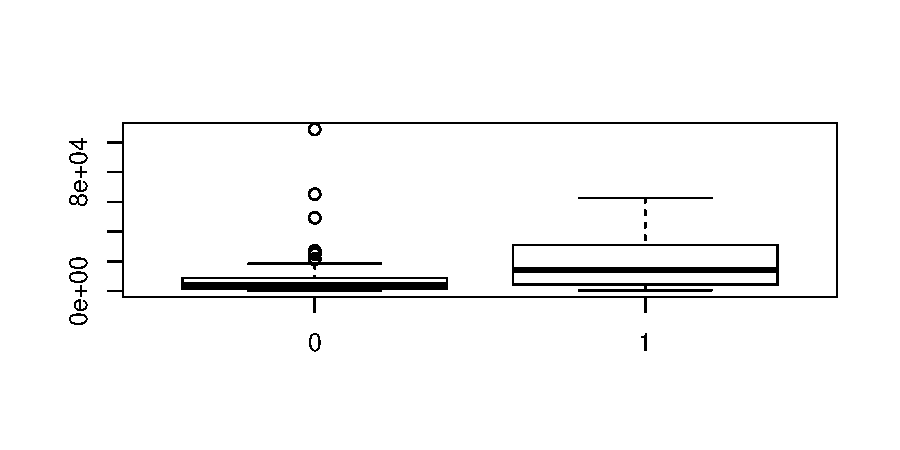
\includegraphics{Kor_BasicStats_files/figure-latex/unnamed-chunk-131-1} \end{center}

\begin{Shaded}
\begin{Highlighting}[]
\NormalTok{QOG  }\OperatorTok\StringTok{ }\KeywordTok{drop_na}\NormalTok{(democracy) }\OperatorTok\StringTok{ }
\StringTok{  }\KeywordTok{ggplot}\NormalTok{(}\KeywordTok{aes}\NormalTok{(}\DataTypeTok{y =}\NormalTok{ gle_cgdpc, }\DataTypeTok{x =} \KeywordTok{as.factor}\NormalTok{(democracy))) }\OperatorTok{+}\StringTok{ }
\StringTok{  }\KeywordTok{geom_boxplot}\NormalTok{() }\OperatorTok{+}\StringTok{ }
\StringTok{  }\KeywordTok{labs}\NormalTok{(}\DataTypeTok{x =} \StringTok{"Regime type"}\NormalTok{, }\DataTypeTok{y =} \StringTok{"GDPPC by constant 2010 US dollars"}\NormalTok{) }\OperatorTok{+}
\StringTok{  }\KeywordTok{scale_x_discrete}\NormalTok{(}\DataTypeTok{labels=}\KeywordTok{c}\NormalTok{(}\StringTok{"0"}\NormalTok{ =}\StringTok{ "Non democracy"}\NormalTok{, }\StringTok{"1"}\NormalTok{ =}\StringTok{ "Democracy"}\NormalTok{)) }\OperatorTok{+}\StringTok{ }
\StringTok{  }\KeywordTok{scale_y_continuous}\NormalTok{(}\DataTypeTok{labels =}\NormalTok{ scales}\OperatorTok{::}\KeywordTok{dollar_format}\NormalTok{()) }\OperatorTok{+}\StringTok{ }
\StringTok{  }\KeywordTok{theme}\NormalTok{(}
    \DataTypeTok{axis.title.x =} \KeywordTok{element_text}\NormalTok{(}\DataTypeTok{margin =} \KeywordTok{margin}\NormalTok{(}\DataTypeTok{t =} \DecValTok{20}\NormalTok{, }\DataTypeTok{b =} \DecValTok{10}\NormalTok{)),}
    \DataTypeTok{axis.title.y =} \KeywordTok{element_text}\NormalTok{(}\DataTypeTok{margin =} \KeywordTok{margin}\NormalTok{(}\DataTypeTok{r =} \DecValTok{20}\NormalTok{, }\DataTypeTok{l =} \DecValTok{20}\NormalTok{))) }\OperatorTok{+}
\StringTok{  }\KeywordTok{guides}\NormalTok{(}\DataTypeTok{fill=}\OtherTok{FALSE}\NormalTok{) }\OperatorTok{+}\StringTok{ }\KeywordTok{theme_bw}\NormalTok{()}
\end{Highlighting}
\end{Shaded}

\begin{center}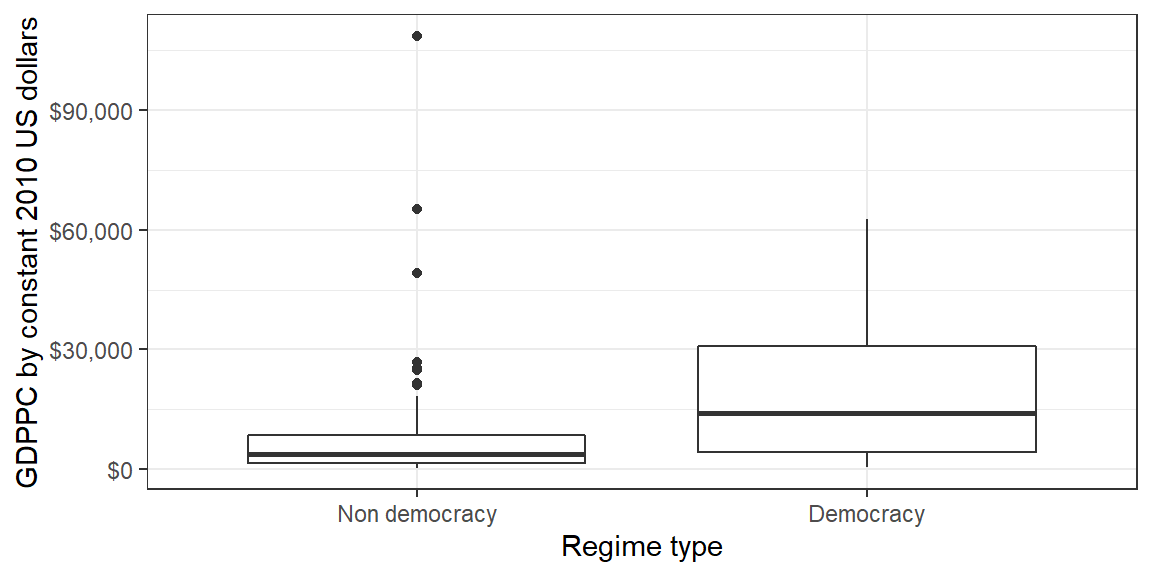
\includegraphics{Kor_BasicStats_files/figure-latex/unnamed-chunk-131-2} \end{center}

과연 이 두 평균의 차이가 통계적으로 유의미한지를 결정하기 위해서 t-검정을 해보고자 합니다. t-검정의 기본적인 개념은 하나의 공식으로 보면:\[
\text{t-statistics} = \frac{(\mu_A - \mu_B) - \text{(NULL: 0)}}{se_A - se_B}\]
라고 할 수 있습니다. 다시 풀어서 말하자면 집단 A와 집단 B의 차이\footnote{엄밀하게 말하면 두 집단의 평균 차이에서 0을 또 빼기 때문에 두 집단의 차이와 0이 다른지 여부를 보는 것이다.}가 각 집단의 평균이 표집을 통해 보일 수 있는 표본 추출로 인해 발생할 수 밖에 없는 평균의 차이\footnote{표준오차는 여러 번 표본들 하나의 모집단으로 뽑았을 때, 그 각 표본의 평균들 간의 표준편차를 의미한다. 따라서 모집단에서 표본을 뽑음으로써 필연적으로 발생할 수밖에 없는 표본들의 평균의 차이들의 평균을 의미한다.}에 비하여 얼마나 큰지를 보는 것입니다. 즉, 일종의 비율입니다.

더 단순하게 말하자면: 두 집단이 정말로 차이가 있을지(평균 차이)를 두 집단이 표본이기 때문에 나타날 수 있는 평균의 차이로 인한 차이(표준오차)와 비교하여 보는 것입니다. 만약 두 집단의 평균 차이가 유의미하게 평균 차이의 표준오차보다 크다면, 이 두 집단은 각 집단의 평균이 표집으로 인해 우연으로 차이가 나타났다기 보다는 정말 차이가 있기 때문에 그런 결과로 나타났을 가능성을 시사합니다.

시작할 때, 비록 민주주의의 1인당 GDP가 비민주주의와는 다를 것이다/혹은 더 높을 것이라는 단측꼬리 가설을 검증하고자 했지만, 여기서의 분석은 양측꼬리 검정(차이가 있다 없다만 보여주는)을 해보도록 하겠습니다.

\begin{Shaded}
\begin{Highlighting}[]
\CommentTok{## 먼저 필요한 통계치들과 표본의 크기를 구해보겠습니다.}
\CommentTok{## 먼저 평균과 표준편차가 필요합니다.}
\NormalTok{mean.dem <-}\StringTok{ }\KeywordTok{mean}\NormalTok{(QOG}\OperatorTok{$}\NormalTok{gle_cgdpc[QOG}\OperatorTok{$}\NormalTok{democracy }\OperatorTok{==}\StringTok{ }\DecValTok{1}\NormalTok{], }\CommentTok{# 민주주의 국가들의 GDPPC 평균}
                 \DataTypeTok{na.rm =} \OtherTok{TRUE}\NormalTok{)}
\NormalTok{mean.nondem <-}\StringTok{ }\KeywordTok{mean}\NormalTok{(QOG}\OperatorTok{$}\NormalTok{gle_cgdpc[QOG}\OperatorTok{$}\NormalTok{democracy }\OperatorTok{==}\StringTok{ }\DecValTok{0}\NormalTok{], }\CommentTok{# 비민주주의}
                    \DataTypeTok{na.rm =} \OtherTok{TRUE}\NormalTok{)}
\NormalTok{sd.dem <-}\StringTok{ }\KeywordTok{sd}\NormalTok{(QOG}\OperatorTok{$}\NormalTok{gle_cgdpc[QOG}\OperatorTok{$}\NormalTok{democracy }\OperatorTok{==}\StringTok{ }\DecValTok{1}\NormalTok{], }\CommentTok{# 민주주의 국가들의 GDPPC SD}
             \DataTypeTok{na.rm =} \OtherTok{TRUE}\NormalTok{)                      }
\NormalTok{sd.nondem <-}\StringTok{ }\KeywordTok{sd}\NormalTok{(QOG}\OperatorTok{$}\NormalTok{gle_cgdpc[QOG}\OperatorTok{$}\NormalTok{democracy }\OperatorTok{==}\StringTok{ }\DecValTok{0}\NormalTok{], }\CommentTok{# sd: standard deviation}
                \DataTypeTok{na.rm =} \OtherTok{TRUE}\NormalTok{)}
\end{Highlighting}
\end{Shaded}

표본의 크기를 구해보겠습니다. \texttt{length()}는 결측치까지 포함해서 관측치의 수를 구하기 때문에 매뉴얼대로 하나하나 통계치를 구해 \texttt{t} 값을 구하려는 지금은 반드시 결측치를 제외하고 계산하는 옵션을 추가해주어야 합니다.

\begin{Shaded}
\begin{Highlighting}[]
\NormalTok{n.dem <-}\StringTok{ }\KeywordTok{length}\NormalTok{(QOG}\OperatorTok{$}\NormalTok{wdi_gdpcapcon2010[QOG}\OperatorTok{$}\NormalTok{democracy }\OperatorTok{==}\StringTok{ }\DecValTok{1} \OperatorTok{&}\StringTok{ }
\StringTok{                                        }\KeywordTok{is.na}\NormalTok{(QOG}\OperatorTok{$}\NormalTok{democracy) }\OperatorTok{==}\StringTok{ }\OtherTok{FALSE} \OperatorTok{&}
\StringTok{                                        }\KeywordTok{is.na}\NormalTok{(QOG}\OperatorTok{$}\NormalTok{wdi_gdpcapcon2010) }\OperatorTok{==}\StringTok{ }\OtherTok{FALSE}\NormalTok{])}
\NormalTok{n.nondem <-}\StringTok{ }\KeywordTok{length}\NormalTok{(QOG}\OperatorTok{$}\NormalTok{wdi_gdpcapcon2010[QOG}\OperatorTok{$}\NormalTok{democracy }\OperatorTok{==}\StringTok{ }\DecValTok{0} \OperatorTok{&}\StringTok{ }
\StringTok{                                           }\KeywordTok{is.na}\NormalTok{(QOG}\OperatorTok{$}\NormalTok{democracy) }\OperatorTok{==}\StringTok{ }\OtherTok{FALSE} \OperatorTok{&}
\StringTok{                                           }\KeywordTok{is.na}\NormalTok{(QOG}\OperatorTok{$}\NormalTok{wdi_gdpcapcon2010) }\OperatorTok{==}\StringTok{ }\OtherTok{FALSE}\NormalTok{])}
\end{Highlighting}
\end{Shaded}

이번에는 두 집단의 차이에 대한 표준오차를 구해보겠습니다.

\begin{Shaded}
\begin{Highlighting}[]
\NormalTok{se.dnd <-}\StringTok{ }\KeywordTok{sqrt}\NormalTok{((sd.dem}\OperatorTok{^}\DecValTok{2} \OperatorTok{/}\StringTok{ }\NormalTok{n.dem) }\OperatorTok{+}\StringTok{ }\NormalTok{(sd.nondem}\OperatorTok{^}\DecValTok{2}\OperatorTok{/}\NormalTok{n.nondem))}
\CommentTok{# The t statistic is calculated easily using these saved values}
\NormalTok{t <-}\StringTok{ }\NormalTok{((mean.dem }\OperatorTok{-}\StringTok{ }\NormalTok{mean.nondem) }\OperatorTok{-}\StringTok{ }\DecValTok{0}\NormalTok{) }\OperatorTok{/}\StringTok{ }\NormalTok{se.dnd}
\NormalTok{t}
\end{Highlighting}
\end{Shaded}

\begin{verbatim}
## [1] 4.03403
\end{verbatim}

두 집단의 평균이 다를 것이라는 대안가설(Alternative hypothesis, \(H_A\))에 대한 유의수준(p-value)는 아래와 같이 계산할 수 있습니다. 여기서는 \textbf{R}에 내장된 굉장히 기본적인 함수들을 조합해서 수학적 공식을 재현하는 것이기 때문에 자유도(degree of freedom)를 대략적으로 구했지만 \textbf{R}에 내장된 \texttt{t-test} 함수는 수학적으로 더 정확하게 계산할 것입니다.

\begin{itemize}
\item
  대안가설(\(H_A\)): 두 집단의 평균이 다를 것이다.

\begin{Shaded}
\begin{Highlighting}[]
\DecValTok{2} \OperatorTok{*}\StringTok{ }\NormalTok{(}\DecValTok{1} \OperatorTok{-}\StringTok{ }\KeywordTok{pt}\NormalTok{(t, }\DataTypeTok{df =} \KeywordTok{min}\NormalTok{(n.dem }\OperatorTok{-}\StringTok{ }\DecValTok{1}\NormalTok{, n.nondem }\OperatorTok{-}\StringTok{ }\DecValTok{1}\NormalTok{)))}
\end{Highlighting}
\end{Shaded}

\begin{verbatim}
## [1] 0.0001281259
\end{verbatim}
\item
  대안가설(\(H_A\)): 민주주의의 1인당 GDP가 비민주주의에 비하여 더 높을 것이다.

\begin{Shaded}
\begin{Highlighting}[]
\NormalTok{(}\DecValTok{1} \OperatorTok{-}\StringTok{ }\KeywordTok{pt}\NormalTok{(t, }\DataTypeTok{df =} \KeywordTok{min}\NormalTok{(n.dem }\OperatorTok{-}\StringTok{ }\DecValTok{1}\NormalTok{, n.nondem }\OperatorTok{-}\StringTok{ }\DecValTok{1}\NormalTok{)))}
\end{Highlighting}
\end{Shaded}

\begin{verbatim}
## [1] 6.406297e-05
\end{verbatim}
\end{itemize}

여기서 생각해볼 문제: 왜 1에서 제외하는 방식을 사용할까? 그리고 왜 2를 곱하는 것일까?

\begin{itemize}
\tightlist
\item
  1을 제외하는 이유는 \textbf{R}은 기본값에 따라서 자동적으로 분포에 있어서 왼쪽으로부터 확률을 계산하기 때문입니다.
\item
  2를 곱하는 이유는 여기서 우리는 방향성을 무시하고 두 집단의 평균 차이가 있는지 없는지의 양측꼬리 검정을 하고자 하기 때문입니다.
\end{itemize}

위에서 여러 단계에 걸쳐서 작성한 \textbf{R} 코드를 다음과 같이 하나의 복잡한 코드로 재구성할 수 있습니다. 다만 이런 경우에는 코드에 에러가 있을 때, 수정이 쉽지 않습니다.

\begin{Shaded}
\begin{Highlighting}[]
\NormalTok{t.alt <-}\StringTok{ }\NormalTok{(}\KeywordTok{mean}\NormalTok{(QOG}\OperatorTok{$}\NormalTok{gle_cgdpc[QOG}\OperatorTok{$}\NormalTok{democracy }\OperatorTok{==}\StringTok{ }\DecValTok{1}\NormalTok{], }
               \DataTypeTok{na.rm =} \OtherTok{TRUE}\NormalTok{) }\OperatorTok{-}\StringTok{ }
\StringTok{            }\KeywordTok{mean}\NormalTok{(QOG}\OperatorTok{$}\NormalTok{gle_cgdpc[QOG}\OperatorTok{$}\NormalTok{democracy }\OperatorTok{==}\StringTok{ }\DecValTok{0}\NormalTok{], }
                 \DataTypeTok{na.rm =} \OtherTok{TRUE}\NormalTok{) }\OperatorTok{-}\StringTok{ }\DecValTok{0}\NormalTok{) }\OperatorTok{/}\StringTok{ }
\StringTok{  }\KeywordTok{sqrt}\NormalTok{(}
\NormalTok{        (}
          \KeywordTok{sd}\NormalTok{(QOG}\OperatorTok{$}\NormalTok{gle_cgdpc[QOG}\OperatorTok{$}\NormalTok{democracy }\OperatorTok{==}\StringTok{ }\DecValTok{1}\NormalTok{], }
             \DataTypeTok{na.rm =} \OtherTok{TRUE}\NormalTok{)}\OperatorTok{^}\DecValTok{2} \OperatorTok{/}\StringTok{ }
\StringTok{            }\KeywordTok{length}\NormalTok{(QOG}\OperatorTok{$}\NormalTok{gle_cgdpc[QOG}\OperatorTok{$}\NormalTok{democracy }\OperatorTok{==}\StringTok{ }\DecValTok{1} \OperatorTok{&}\StringTok{ }
\StringTok{                                           }\KeywordTok{is.na}\NormalTok{(QOG}\OperatorTok{$}\NormalTok{democracy) }\OperatorTok{==}\StringTok{ }\OtherTok{FALSE} \OperatorTok{&}
\StringTok{            }\KeywordTok{is.na}\NormalTok{(QOG}\OperatorTok{$}\NormalTok{gle_cgdpc) }\OperatorTok{==}\StringTok{ }\OtherTok{FALSE}\NormalTok{])}
\NormalTok{        ) }\OperatorTok{+}
\StringTok{        }\NormalTok{(}
          \KeywordTok{sd}\NormalTok{(QOG}\OperatorTok{$}\NormalTok{gle_cgdpc[QOG}\OperatorTok{$}\NormalTok{democracy }\OperatorTok{==}\StringTok{ }\DecValTok{0}\NormalTok{], }
             \DataTypeTok{na.rm =} \OtherTok{TRUE}\NormalTok{)}\OperatorTok{^}\DecValTok{2} \OperatorTok{/}\StringTok{ }
\StringTok{            }\KeywordTok{length}\NormalTok{(QOG}\OperatorTok{$}\NormalTok{gle_cgdpc[QOG}\OperatorTok{$}\NormalTok{democracy }\OperatorTok{==}\StringTok{ }\DecValTok{0} \OperatorTok{&}\StringTok{ }
\StringTok{                                           }\KeywordTok{is.na}\NormalTok{(QOG}\OperatorTok{$}\NormalTok{democracy) }\OperatorTok{==}\StringTok{ }\OtherTok{FALSE} \OperatorTok{&}
\StringTok{            }\KeywordTok{is.na}\NormalTok{(QOG}\OperatorTok{$}\NormalTok{gle_cgdpc) }\OperatorTok{==}\StringTok{ }\OtherTok{FALSE}\NormalTok{])}
\NormalTok{        )}
\NormalTok{      )}
\NormalTok{t.alt}
\end{Highlighting}
\end{Shaded}

\begin{verbatim}
## [1] 4.082703
\end{verbatim}

\hypertarget{ruxb85c-uxd560-uxc218-uxc788uxb294-t-test-uxb450-uxac00uxc9c0-uxbc29uxbc95}{%
\subsubsection{\texorpdfstring{\textbf{R}로 할 수 있는 t-test: 두 가지 방법}{R로 할 수 있는 t-test: 두 가지 방법}}\label{ruxb85c-uxd560-uxc218-uxc788uxb294-t-test-uxb450-uxac00uxc9c0-uxbc29uxbc95}}

\begin{enumerate}
\def\labelenumi{\arabic{enumi}.}
\tightlist
\item
  만약 각각의 집단에 대한 서로 다른 두 데이터를 가지고 있다면 유용한 방법
\end{enumerate}

\begin{Shaded}
\begin{Highlighting}[]
\NormalTok{ttest1 <-}\StringTok{ }\KeywordTok{t.test}\NormalTok{(QOG}\OperatorTok{$}\NormalTok{gle_cgdpc[QOG}\OperatorTok{$}\NormalTok{democracy }\OperatorTok{==}\StringTok{ }\DecValTok{1}\NormalTok{],}
\NormalTok{                 QOG}\OperatorTok{$}\NormalTok{gle_cgdpc[QOG}\OperatorTok{$}\NormalTok{democracy }\OperatorTok{==}\StringTok{ }\DecValTok{0}\NormalTok{])}
\NormalTok{ttest1}
\end{Highlighting}
\end{Shaded}

\begin{verbatim}
## 
##    Welch Two Sample t-test
## 
## data:  QOG$gle_cgdpc[QOG$democracy == 1] and QOG$gle_cgdpc[QOG$democracy == 0]
## t = 4.0827, df = 159.85, p-value = 7.017e-05
## alternative hypothesis: true difference in means is not equal to 0
## 95 percent confidence interval:
##   5008.492 14394.022
## sample estimates:
## mean of x mean of y 
## 18081.991  8380.733
\end{verbatim}

\begin{itemize}
\tightlist
\item
  \texttt{t.test()} 함수는 앞서서는 직접 제거해줘야 했던 결측치의 문제를 자동으로 처리해주는 기본값을 가지고 있습니다.
\end{itemize}

\begin{enumerate}
\def\labelenumi{\arabic{enumi}.}
\setcounter{enumi}{1}
\tightlist
\item
  두 번째 방법은 두 집단이 하나의 데이터에 같이 있을 때 유용한 방법입니다.
\end{enumerate}

\begin{Shaded}
\begin{Highlighting}[]
\NormalTok{ttest2 <-}\StringTok{ }\KeywordTok{t.test}\NormalTok{(gle_cgdpc }\OperatorTok{~}\StringTok{ }\NormalTok{democracy, }\DataTypeTok{data =}\NormalTok{ QOG)}
\NormalTok{ttest2}
\end{Highlighting}
\end{Shaded}

\begin{verbatim}
## 
##    Welch Two Sample t-test
## 
## data:  gle_cgdpc by democracy
## t = -4.0827, df = 159.85, p-value = 7.017e-05
## alternative hypothesis: true difference in means is not equal to 0
## 95 percent confidence interval:
##  -14394.022  -5008.492
## sample estimates:
## mean in group 0 mean in group 1 
##        8380.733       18081.991
\end{verbatim}

\begin{itemize}
\tightlist
\item
  역시 \texttt{t.test()} 함수를 이용하지만 각 집단의 차이를 규정하는 변수(group identifier)가 있을 때 용이한 방법입니다.
\end{itemize}

\hypertarget{uxbd84uxc0b0uxbd84uxc11danovauxc744-uxc774uxc6a9uxd574-uxc5ecuxb7ec-uxd3c9uxade0uxc744-uxbe44uxad50uxd558uxae30}{%
\subsection{분산분석(ANOVA)을 이용해 여러 평균을 비교하기}\label{uxbd84uxc0b0uxbd84uxc11danovauxc744-uxc774uxc6a9uxd574-uxc5ecuxb7ec-uxd3c9uxade0uxc744-uxbe44uxad50uxd558uxae30}}

이번에는 \texttt{CIRI} 데이터를 이용해 국가들의 ``고문''(torture) 유형에 따라서 1인당 GDP의 차이가 어떻게 나타나는지를 살펴보겠습니다. 먼저 고문의 유형을 분류해보겠습니다.

\begin{itemize}
\tightlist
\item
  0은 50건 이상의 고문 사례가 있는 경우
\item
  1은 1건에서 49건 사이 사례를 가지는 경우
\item
  2는 보고된 고문 사례가 아예 없는 경우입니다.
\end{itemize}

\begin{Shaded}
\begin{Highlighting}[]
\NormalTok{knitr}\OperatorTok{::}\KeywordTok{kable}\NormalTok{(}\KeywordTok{table}\NormalTok{(QOG}\OperatorTok{$}\NormalTok{ciri_tort))}
\end{Highlighting}
\end{Shaded}

\begin{tabular}{l|r}
\hline
Var1 & Freq\\
\hline
0 & 86\\
\hline
1 & 75\\
\hline
2 & 31\\
\hline
\end{tabular}

고문 유형에 따른 1인당 GDP의 분포를 그래프로 나타내 보겠습니다.

\begin{Shaded}
\begin{Highlighting}[]
\KeywordTok{boxplot}\NormalTok{(gle_cgdpc }\OperatorTok{~}\StringTok{ }\NormalTok{ciri_tort, }\DataTypeTok{data =}\NormalTok{ QOG)}
\end{Highlighting}
\end{Shaded}

\begin{center}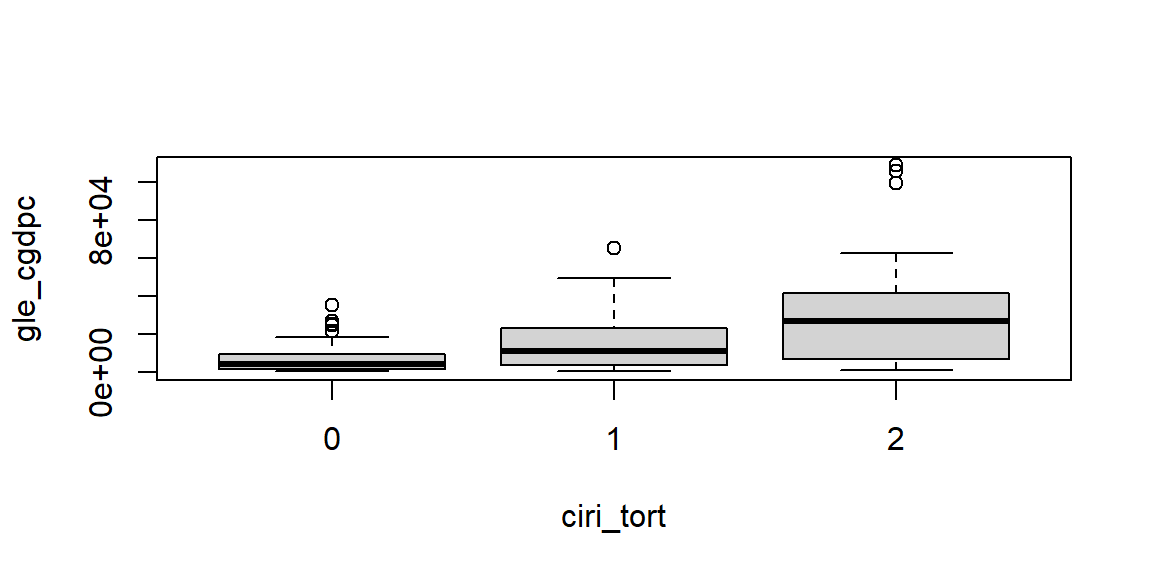
\includegraphics{Kor_BasicStats_files/figure-latex/unnamed-chunk-141-1} \end{center}

\begin{Shaded}
\begin{Highlighting}[]
\NormalTok{QOG  }\OperatorTok\StringTok{ }\KeywordTok{drop_na}\NormalTok{(ciri_tort) }\OperatorTok\StringTok{ }
\StringTok{  }\KeywordTok{ggplot}\NormalTok{(}\KeywordTok{aes}\NormalTok{(}\DataTypeTok{y =}\NormalTok{ gle_cgdpc, }\DataTypeTok{x =} \KeywordTok{as.factor}\NormalTok{(ciri_tort))) }\OperatorTok{+}\StringTok{ }
\StringTok{  }\KeywordTok{geom_boxplot}\NormalTok{() }\OperatorTok{+}\StringTok{ }
\StringTok{  }\KeywordTok{labs}\NormalTok{(}\DataTypeTok{x =} \StringTok{"Torture type"}\NormalTok{, }\DataTypeTok{y =} \StringTok{"GDPPC by constant 2010 US dollars"}\NormalTok{) }\OperatorTok{+}
\StringTok{  }\KeywordTok{scale_x_discrete}\NormalTok{(}\DataTypeTok{labels=}\KeywordTok{c}\NormalTok{(}\StringTok{"0"}\NormalTok{ =}\StringTok{ "Torture (+50)"}\NormalTok{, }
                            \StringTok{"1"}\NormalTok{ =}\StringTok{ "Torture (1-49)"}\NormalTok{,}
                            \StringTok{"2"}\NormalTok{ =}\StringTok{ "No torture"}\NormalTok{)) }\OperatorTok{+}
\StringTok{  }\KeywordTok{scale_y_continuous}\NormalTok{(}\DataTypeTok{labels =}\NormalTok{ scales}\OperatorTok{::}\KeywordTok{dollar_format}\NormalTok{()) }\OperatorTok{+}\StringTok{ }
\StringTok{  }\KeywordTok{theme}\NormalTok{(}
    \DataTypeTok{axis.title.x =} \KeywordTok{element_text}\NormalTok{(}\DataTypeTok{margin =} \KeywordTok{margin}\NormalTok{(}\DataTypeTok{t =} \DecValTok{20}\NormalTok{, }\DataTypeTok{b =} \DecValTok{10}\NormalTok{)),}
    \DataTypeTok{axis.title.y =} \KeywordTok{element_text}\NormalTok{(}\DataTypeTok{margin =} \KeywordTok{margin}\NormalTok{(}\DataTypeTok{r =} \DecValTok{20}\NormalTok{, }\DataTypeTok{l =} \DecValTok{10}\NormalTok{))) }\OperatorTok{+}
\StringTok{  }\KeywordTok{guides}\NormalTok{(}\DataTypeTok{fill=}\OtherTok{FALSE}\NormalTok{) }\OperatorTok{+}\StringTok{ }\KeywordTok{theme_bw}\NormalTok{()}
\end{Highlighting}
\end{Shaded}

\begin{center}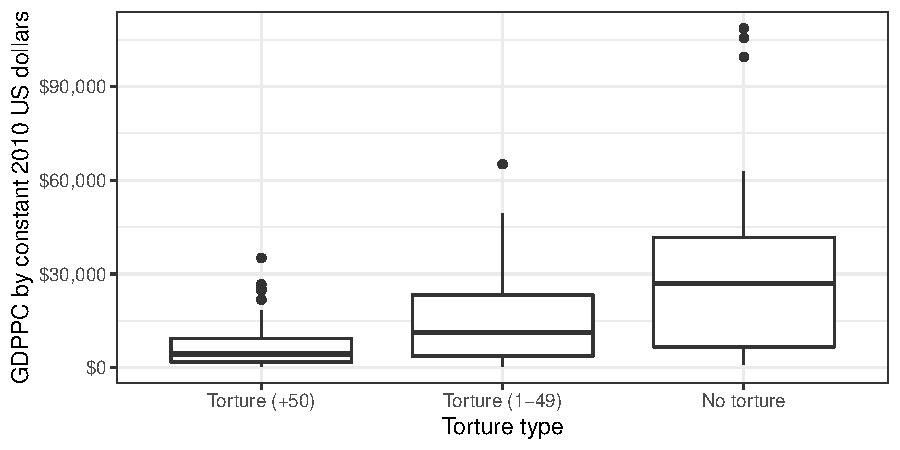
\includegraphics{Kor_BasicStats_files/figure-latex/unnamed-chunk-141-2} \end{center}

적어도 박스플롯은 세 집단의 평균에 유의미한 차이가 있을 수도 있다고 기대하게 합니다. 이제는 분산분석을 해봅시다. 이번에는 \textbf{R}에서 제공하는 분산분석 함수를 이용해보도록 하겠습니다.

\begin{Shaded}
\begin{Highlighting}[]
\NormalTok{model1 <-}\StringTok{ }\KeywordTok{aov}\NormalTok{(gle_cgdpc }\OperatorTok{~}\StringTok{ }\KeywordTok{as.factor}\NormalTok{(ciri_tort), }\DataTypeTok{data =}\NormalTok{ QOG)}
\KeywordTok{summary}\NormalTok{(model1) }
\end{Highlighting}
\end{Shaded}

\begin{verbatim}
##                       Df    Sum Sq   Mean Sq F value   Pr(>F)    
## as.factor(ciri_tort)   2 1.386e+10 6.932e+09   28.03 2.18e-11 ***
## Residuals            189 4.674e+10 2.473e+08                     
## ---
## Signif. codes:  0 '***' 0.001 '**' 0.01 '*' 0.05 '.' 0.1 ' ' 1
## 19 observations deleted due to missingness
\end{verbatim}

결과적으로 ANOVA의 결과는 유의수준(P-value, 여기서는 \texttt{Pr(\textgreater{}F)})의 값이 매우 작게 나와 영가설(\(H_0: \mu_1 = \mu_2 = \mu_3, \cdots, \mu_n\))이 기각된 것을 확인할 수 있습니다. 그렇다면 만약 정치체제와 고문유형별로 집단을 더 쪼개어보면 어떻게 될까요?

\begin{Shaded}
\begin{Highlighting}[]
\CommentTok{## 먼저, 쪼갠 집단별로 그래프를 그려보겠습니다.}
\KeywordTok{boxplot}\NormalTok{(gle_cgdpc }\OperatorTok{~}\StringTok{ }\NormalTok{ciri_tort}\OperatorTok{:}\NormalTok{democracy, }\DataTypeTok{data =}\NormalTok{ QOG) }\CommentTok{## 콜론(:)은 상호작용을 보여줍니다.}
\end{Highlighting}
\end{Shaded}

\begin{center}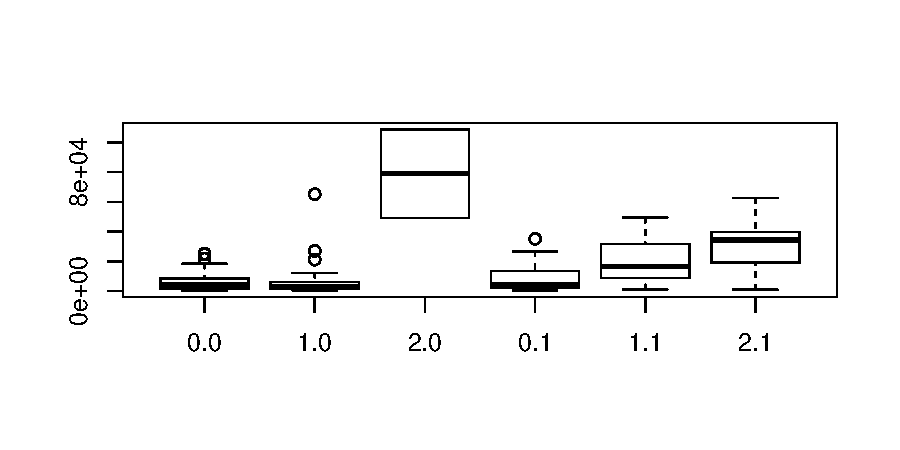
\includegraphics{Kor_BasicStats_files/figure-latex/unnamed-chunk-143-1} \end{center}

\begin{Shaded}
\begin{Highlighting}[]
\CommentTok{## 그런데 기본 플롯으로 그리면 x축이 가독성이 떨어집니다.}
\NormalTok{QOG }\OperatorTok\StringTok{ }\KeywordTok{drop_na}\NormalTok{(ciri_tort) }\OperatorTok\StringTok{ }\KeywordTok{drop_na}\NormalTok{(democracy) }\OperatorTok
\StringTok{  }\KeywordTok{ggplot}\NormalTok{(}\KeywordTok{aes}\NormalTok{(}\DataTypeTok{y=}\NormalTok{gle_cgdpc, }\DataTypeTok{x=}\KeywordTok{as.factor}\NormalTok{(ciri_tort)}\OperatorTok{:}\KeywordTok{as.factor}\NormalTok{(democracy),}
             \DataTypeTok{group=}\KeywordTok{interaction}\NormalTok{(democracy, ciri_tort))) }\OperatorTok{+}\StringTok{ }\KeywordTok{geom_boxplot}\NormalTok{() }\OperatorTok{+}\StringTok{ }
\StringTok{  }\KeywordTok{labs}\NormalTok{(}\DataTypeTok{x =} \StringTok{"Torture X Regime type"}\NormalTok{, }\DataTypeTok{y =} \StringTok{"GDPPC by constant 2010 US dollars"}\NormalTok{) }\OperatorTok{+}
\StringTok{  }\KeywordTok{scale_x_discrete}\NormalTok{(}\DataTypeTok{labels=}\KeywordTok{c}\NormalTok{(}\StringTok{"0:0"}\NormalTok{ =}\StringTok{ "Torture (+50)}\CharTok{\textbackslash{}n}\StringTok{Non Democracy"}\NormalTok{, }
                            \StringTok{"0:1"}\NormalTok{ =}\StringTok{ "Torture (+50)}\CharTok{\textbackslash{}n}\StringTok{Democracy"}\NormalTok{, }
                            \StringTok{"1:0"}\NormalTok{ =}\StringTok{ "Torture (1-49)}\CharTok{\textbackslash{}n}\StringTok{Non Democracy"}\NormalTok{,}
                            \StringTok{"1:1"}\NormalTok{ =}\StringTok{ "Torture (1-49)}\CharTok{\textbackslash{}n}\StringTok{Democracy"}\NormalTok{,}
                            \StringTok{"2:0"}\NormalTok{ =}\StringTok{ "No torture}\CharTok{\textbackslash{}n}\StringTok{Non Democracy"}\NormalTok{,}
                            \StringTok{"2:1"}\NormalTok{ =}\StringTok{ "No torture}\CharTok{\textbackslash{}n}\StringTok{Democracy"}\NormalTok{)) }\OperatorTok{+}
\StringTok{  }\KeywordTok{scale_y_continuous}\NormalTok{(}\DataTypeTok{labels =}\NormalTok{ scales}\OperatorTok{::}\KeywordTok{dollar_format}\NormalTok{()) }\OperatorTok{+}\StringTok{ }
\StringTok{  }\KeywordTok{theme}\NormalTok{(}
    \DataTypeTok{axis.title.x =} \KeywordTok{element_text}\NormalTok{(}\DataTypeTok{margin =} \KeywordTok{margin}\NormalTok{(}\DataTypeTok{t =} \DecValTok{15}\NormalTok{, }\DataTypeTok{b =} \DecValTok{10}\NormalTok{)),}
    \DataTypeTok{axis.title.y =} \KeywordTok{element_text}\NormalTok{(}\DataTypeTok{margin =} \KeywordTok{margin}\NormalTok{(}\DataTypeTok{r =} \DecValTok{20}\NormalTok{, }\DataTypeTok{l =} \DecValTok{10}\NormalTok{)),}
    \DataTypeTok{axis.text.x =} \KeywordTok{element_text}\NormalTok{(}\DataTypeTok{margin =} \KeywordTok{margin}\NormalTok{(}\DataTypeTok{t =} \DecValTok{10}\NormalTok{))) }\OperatorTok{+}
\StringTok{  }\KeywordTok{guides}\NormalTok{(}\DataTypeTok{fill=}\OtherTok{FALSE}\NormalTok{) }\OperatorTok{+}\StringTok{ }\KeywordTok{theme_bw}\NormalTok{()}
\end{Highlighting}
\end{Shaded}

\begin{center}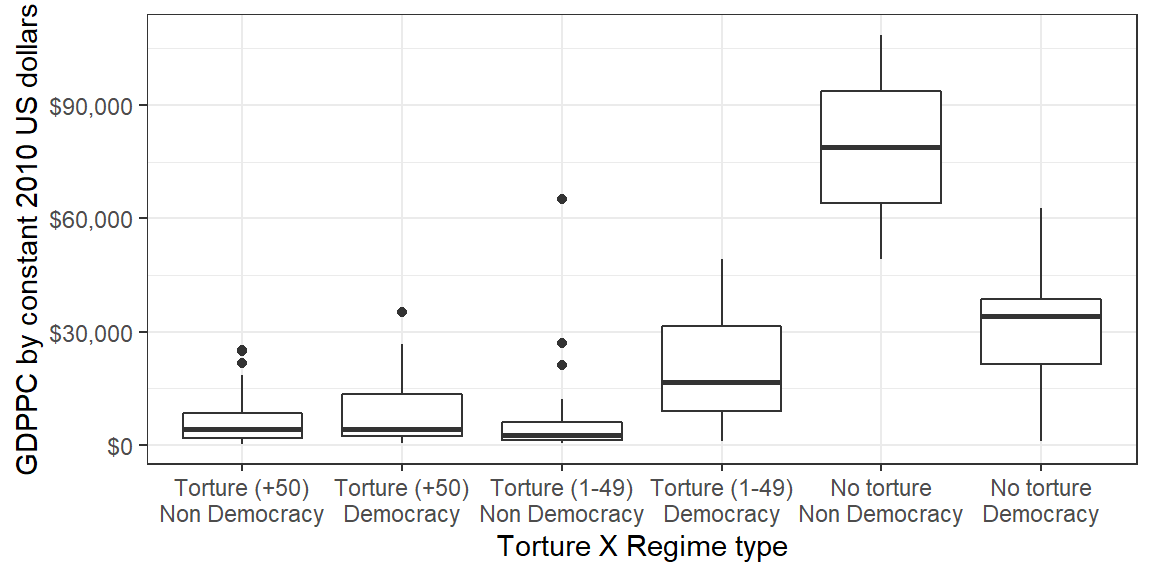
\includegraphics{Kor_BasicStats_files/figure-latex/unnamed-chunk-143-2} \end{center}

이렇게 두 개 유형의 조합을 분산분석하기 위해서는 마찬가지로 \texttt{aov()} 함수에 두 요인형 변수의 상호작용을 콜론(\texttt{:})을 이용해 포함해주면 됩니다.

\begin{Shaded}
\begin{Highlighting}[]
\NormalTok{model2 <-}\StringTok{ }\KeywordTok{aov}\NormalTok{(gle_cgdpc }\OperatorTok{~}\StringTok{ }\KeywordTok{as.factor}\NormalTok{(ciri_tort)}\OperatorTok{:}\KeywordTok{as.factor}\NormalTok{(democracy), }\DataTypeTok{data =}\NormalTok{ QOG)}
\KeywordTok{summary}\NormalTok{(model2) }
\end{Highlighting}
\end{Shaded}

\begin{verbatim}
##                                            Df    Sum Sq   Mean Sq F value
## as.factor(ciri_tort):as.factor(democracy)   5 1.851e+10 3.703e+09   26.09
## Residuals                                 156 2.214e+10 1.419e+08        
##                                           Pr(>F)    
## as.factor(ciri_tort):as.factor(democracy) <2e-16 ***
## Residuals                                           
## ---
## Signif. codes:  0 '***' 0.001 '**' 0.01 '*' 0.05 '.' 0.1 ' ' 1
## 49 observations deleted due to missingness
\end{verbatim}

단, 명심해야 할 것은 상호작용의 대상이 되는 변수들은 여기서 집단을 보여주는 요인형 변수여야 한다는 것입니다.

\hypertarget{uxbe44uxc728-uxcc28uxc774-uxad50uxcc28uxd45cuxc640-uxce74uxc774uxc2a4uxd018uxc5b4-uxac80uxc815chi-squared-tests}{%
\section{비율 차이: 교차표와 카이스퀘어 검정(chi-squared tests)}\label{uxbe44uxc728-uxcc28uxc774-uxad50uxcc28uxd45cuxc640-uxce74uxc774uxc2a4uxd018uxc5b4-uxac80uxc815chi-squared-tests}}

자료 유형에 따라서 우리가 확인해야할 통계치도 달라집니다. 예를 들어, 연속형 변수의 경우 대표값을 평균(mean)을 보면 되겠지만 이산형 변수의 경우는 비율을 볼 필요가 있습니다. 동전을 100번 던진다고 할 때, 앞면이 56번, 뒷면이 44번 나온 경우, 사실 평균인 0.56은 앞면이 나올 확률과 동일합니다. 즉, 전체 동전을 던진 횟수에 대한 성공 횟수의 비율인 것입니다.

비율 차이를 확인하고 이 차이의 통계적 유의성을 검정하는 일련의 절차를 확인하기 위하여 두 개의 연도에 걸쳐서 여러 국가들에 걸쳐 수행된 무신론에 관한 설문조사 결과를 다운로드 해보겠습니다.

\begin{Shaded}
\begin{Highlighting}[]
\NormalTok{here}\OperatorTok{::}\KeywordTok{here}\NormalTok{() }\OperatorTok\StringTok{ }\KeywordTok{setwd}\NormalTok{()}
\KeywordTok{download.file}\NormalTok{(}\StringTok{"http://www.openintro.org/stat/data/atheism.RData"}\NormalTok{, }
                \DataTypeTok{destfile =} \StringTok{"atheism.RData"}\NormalTok{)}
\KeywordTok{load}\NormalTok{(}\StringTok{"atheism.RData"}\NormalTok{)}
\end{Highlighting}
\end{Shaded}

이렇게 불러온 데이터를 자세히 살펴보겠습니다.

\begin{Shaded}
\begin{Highlighting}[]
\KeywordTok{glimpse}\NormalTok{(atheism)}
\end{Highlighting}
\end{Shaded}

\begin{verbatim}
## Observations: 88,032
## Variables: 3
## $ nationality <fct> Afghanistan, Afghanistan, Afghanistan, Afghanistan...
## $ response    <fct> non-atheist, non-atheist, non-atheist, non-atheist...
## $ year        <int> 2012, 2012, 2012, 2012, 2012, 2012, 2012, 2012, 20...
\end{verbatim}

\texttt{nationality}는 응답자의 국적을 의미하며 \texttt{year}는 설문조사가 시행된 연도, 마지막으로 \texttt{response}는 응답자가 자신이 무신론자인지 아닌지 등을 응답한 내용입니다. 그럼 응답변수만을 한 번 구체적으로 살펴보겠습니다.

\begin{Shaded}
\begin{Highlighting}[]
\NormalTok{knitr}\OperatorTok{::}\KeywordTok{kable}\NormalTok{(}\KeywordTok{table}\NormalTok{(atheism}\OperatorTok{$}\NormalTok{response))}
\end{Highlighting}
\end{Shaded}

\begin{tabular}{l|r}
\hline
Var1 & Freq\\
\hline
atheist & 5498\\
\hline
non-atheist & 82534\\
\hline
\end{tabular}

교차표를 이용해서 우리는 행과 열에 총계와 비율을 구할 수 있습니다. 이와 같은 빈도/비율표는 변수를 기술하기 위해서 유용하게 사용됩니다.

\begin{Shaded}
\begin{Highlighting}[]
\NormalTok{table1 <-}\StringTok{ }\KeywordTok{table}\NormalTok{(atheism}\OperatorTok{$}\NormalTok{response, atheism}\OperatorTok{$}\NormalTok{year)}

\KeywordTok{margin.table}\NormalTok{(table1, }\DecValTok{1}\NormalTok{) }\OperatorTok\StringTok{ }\NormalTok{knitr}\OperatorTok{::}\KeywordTok{kable}\NormalTok{() }\CommentTok{# 행에 총계를 계산}
\end{Highlighting}
\end{Shaded}

\begin{tabular}{l|r}
\hline
Var1 & Freq\\
\hline
atheist & 5498\\
\hline
non-atheist & 82534\\
\hline
\end{tabular}

\begin{Shaded}
\begin{Highlighting}[]
\KeywordTok{margin.table}\NormalTok{(table1, }\DecValTok{2}\NormalTok{) }\OperatorTok\StringTok{ }\NormalTok{knitr}\OperatorTok{::}\KeywordTok{kable}\NormalTok{() }\CommentTok{# 열에 총계를 계산}
\end{Highlighting}
\end{Shaded}

\begin{tabular}{l|r}
\hline
Var1 & Freq\\
\hline
2005 & 36105\\
\hline
2012 & 51927\\
\hline
\end{tabular}

\begin{Shaded}
\begin{Highlighting}[]
\KeywordTok{prop.table}\NormalTok{(table1, }\DecValTok{1}\NormalTok{) }\OperatorTok\StringTok{ }\NormalTok{knitr}\OperatorTok{::}\KeywordTok{kable}\NormalTok{() }\CommentTok{# 행에 비율을 계산}
\end{Highlighting}
\end{Shaded}

\begin{tabular}{l|r|r}
\hline
  & 2005 & 2012\\
\hline
atheist & 0.3677701 & 0.6322299\\
\hline
non-atheist & 0.4129571 & 0.5870429\\
\hline
\end{tabular}

\begin{Shaded}
\begin{Highlighting}[]
\KeywordTok{prop.table}\NormalTok{(table1, }\DecValTok{2}\NormalTok{) }\OperatorTok\StringTok{ }\NormalTok{knitr}\OperatorTok{::}\KeywordTok{kable}\NormalTok{() }\CommentTok{# 열에 비율을 계산}
\end{Highlighting}
\end{Shaded}

\begin{tabular}{l|r|r}
\hline
  & 2005 & 2012\\
\hline
atheist & 0.0560033 & 0.0669401\\
\hline
non-atheist & 0.9439967 & 0.9330599\\
\hline
\end{tabular}

이번에는 2005년과 2012년 간 미국에서 무신론자의 비율이 변화가 있었는지를 검증해보도록 하겠습니다. 먼저, 미국의 응답자들만을 대상으로 하는 서브셋을 만들어보겠습니다.

\begin{Shaded}
\begin{Highlighting}[]
\NormalTok{us <-}\StringTok{ }\KeywordTok{subset}\NormalTok{(atheism, nationality }\OperatorTok{==}\StringTok{ "United States"}\NormalTok{)}
\end{Highlighting}
\end{Shaded}

이렇게 만든 \texttt{us}라는 서브셋을 가지고 카이스퀘어 검정을 해보고자 합니다.

\begin{Shaded}
\begin{Highlighting}[]
\KeywordTok{prop.test}\NormalTok{(}\KeywordTok{table}\NormalTok{(us}\OperatorTok{$}\NormalTok{year, us}\OperatorTok{$}\NormalTok{response), }\DataTypeTok{correct =} \OtherTok{FALSE}\NormalTok{) }
\end{Highlighting}
\end{Shaded}

\begin{verbatim}
## 
##  2-sample test for equality of proportions without continuity
##  correction
## 
## data:  table(us$year, us$response)
## X-squared = 27.49, df = 1, p-value = 1.579e-07
## alternative hypothesis: two.sided
## 95 percent confidence interval:
##  -0.05474042 -0.02509990
## sample estimates:
##     prop 1     prop 2 
## 0.00998004 0.04990020
\end{verbatim}

위에서 중요한 것이 바로 변수의 순서입니다. 어떤 기준별로 특정 변수를 볼 것인가에 따라 그 기준이 될 변수가 앞으로 가고, 분석의 대상이 될 변수가 뒤로 가는 것입니다. 예를 들어, 위의 \texttt{us} 데이터에서 \texttt{year}와 \texttt{response}의 위치를 바꾸어 보겠습니다.

\begin{Shaded}
\begin{Highlighting}[]
\KeywordTok{prop.test}\NormalTok{(}\KeywordTok{table}\NormalTok{(us}\OperatorTok{$}\NormalTok{response, us}\OperatorTok{$}\NormalTok{year), }\DataTypeTok{correct =} \OtherTok{FALSE}\NormalTok{)}
\end{Highlighting}
\end{Shaded}

\begin{verbatim}
## 
##  2-sample test for equality of proportions without continuity
##  correction
## 
## data:  table(us$response, us$year)
## X-squared = 27.49, df = 1, p-value = 1.579e-07
## alternative hypothesis: two.sided
## 95 percent confidence interval:
##  -0.4405031 -0.2467397
## sample estimates:
##    prop 1    prop 2 
## 0.1666667 0.5102881
\end{verbatim}

첫 번째 코드가 두 개의 연도(2005, 2012) 별로 무신론자에 대한 응답 비율을 비교한 것이었다면, 두 번째는 무신론자냐 비무신론자냐에 따라 연도들의 비율을 비교한 결과입니다. 둘 다 두 개 집단만 가지고 있는 변수라 얼핏 비슷해 보이지만 신뢰구간과 표본 추정치(\texttt{sample\ estimates})를 보면 다른 것을 확인할 수 있습니다.

그리고 한 가지 더 명심해야할 것은 \textbf{R}은 여러 줄의 코드를 중첩하여 사용하는 것도 가능하다는 것입니다. 예를 들어, 위의 코드는 아래와 같이 쓸 수도 있습니다.

\begin{Shaded}
\begin{Highlighting}[]
\NormalTok{ustab <-}\StringTok{ }\KeywordTok{table}\NormalTok{(us}\OperatorTok{$}\NormalTok{year, us}\OperatorTok{$}\NormalTok{response) }\CommentTok{# 아예 교차표를 먼저 저장합니다.}
\KeywordTok{prop.test}\NormalTok{(ustab, }\DataTypeTok{correct =} \OtherTok{FALSE}\NormalTok{)    }\CommentTok{# 그리고 prop.test를 저장된 교차표로 시행합니다.}
\end{Highlighting}
\end{Shaded}

\begin{verbatim}
## 
##  2-sample test for equality of proportions without continuity
##  correction
## 
## data:  ustab
## X-squared = 27.49, df = 1, p-value = 1.579e-07
## alternative hypothesis: two.sided
## 95 percent confidence interval:
##  -0.05474042 -0.02509990
## sample estimates:
##     prop 1     prop 2 
## 0.00998004 0.04990020
\end{verbatim}

\begin{Shaded}
\begin{Highlighting}[]
\CommentTok{# R은 때로는 중첩해서 하나의 코드에 여러 기능이 가능하게끔 하기도 합니다.}
\KeywordTok{prop.test}\NormalTok{(}\KeywordTok{table}\NormalTok{(atheism}\OperatorTok{$}\NormalTok{year[atheism}\OperatorTok{$}\NormalTok{nationality }\OperatorTok{==}\StringTok{ }
\StringTok{                               "United States"}\NormalTok{], }
\NormalTok{                atheism}\OperatorTok{$}\NormalTok{response[atheism}\OperatorTok{$}\NormalTok{nationality }\OperatorTok{==}\StringTok{ }
\StringTok{                                   "United States"}\NormalTok{]), }
          \DataTypeTok{correct =} \OtherTok{FALSE}\NormalTok{)}
\end{Highlighting}
\end{Shaded}

\begin{verbatim}
## 
##  2-sample test for equality of proportions without continuity
##  correction
## 
## data:  table(atheism$year[atheism$nationality == "United States"], atheism$response[atheism$nationality ==     "United States"])
## X-squared = 27.49, df = 1, p-value = 1.579e-07
## alternative hypothesis: two.sided
## 95 percent confidence interval:
##  -0.05474042 -0.02509990
## sample estimates:
##     prop 1     prop 2 
## 0.00998004 0.04990020
\end{verbatim}

자, 이번에는 2012년 미국 총선의 시계열 설문조사에서 자료를 사용해보도록 하겠습니다. 여기 \href{https://github.com/jhomola/PS5/blob/master/anes_timeseries_2012_stata12.dta}{깃허브}에서도 제공하고 있습니다. 다운받았다고 생각하고 진행하겠습니다.

\begin{Shaded}
\begin{Highlighting}[]
\NormalTok{anes <-}\StringTok{ }\KeywordTok{pick}\NormalTok{(}\StringTok{"example.data/anes_timeseries_2012_Stata12.dta"}\NormalTok{)}
\CommentTok{## 데이터가 꽤 규모가 있습니다. 2249개의 변수를 가지고 5914개의 관측치가 있습니다.}
\CommentTok{## 따라서 이렇게 큰 데이터를 사용하기 전에는 코드북을 숙지하여 어떤 변수가}
\CommentTok{## 어떤 것을 측정하고 있는지를 미리 파악해 두셔야 합니다.}
\end{Highlighting}
\end{Shaded}

이렇게 불러온 \texttt{ANES} 자료에서 \texttt{xtabs()} 함수를 이용하여 정당 ID와 2012년에 대통령 후부 누구에게 투표했는지를 보여주는 변수 간의 교차표를 살펴보도록 하겠습니다.

\begin{Shaded}
\begin{Highlighting}[]
\KeywordTok{xtabs}\NormalTok{( }\OperatorTok{~}\StringTok{ }\NormalTok{pid_x }\OperatorTok{+}\StringTok{ }\NormalTok{presvote2012_x, }\DataTypeTok{data =}\NormalTok{ anes) }\OperatorTok\StringTok{ }\NormalTok{knitr}\OperatorTok{::}\KeywordTok{kable}\NormalTok{() }
\end{Highlighting}
\end{Shaded}

\begin{tabular}{l|r|r|r|r|r|r}
\hline
  & -9 & -6 & -2 & 1 & 2 & 5\\
\hline
-2 & 5 & 0 & 8 & 7 & 4 & 0\\
\hline
1 & 7 & 0 & 239 & 1219 & 15 & 5\\
\hline
2 & 8 & 0 & 250 & 519 & 86 & 8\\
\hline
3 & 1 & 0 & 241 & 451 & 35 & 19\\
\hline
4 & 20 & 0 & 390 & 174 & 157 & 51\\
\hline
5 & 3 & 0 & 161 & 47 & 381 & 18\\
\hline
6 & 3 & 0 & 157 & 61 & 387 & 15\\
\hline
7 & 5 & 1 & 109 & 18 & 627 & 2\\
\hline
\end{tabular}

\begin{Shaded}
\begin{Highlighting}[]
\CommentTok{## xtabs()는 만약 두 개 이상 변수들에 대해 살펴보고 싶을 때 유용한 함수입니다.}
\KeywordTok{table}\NormalTok{(anes}\OperatorTok{$}\NormalTok{pid_x, anes}\OperatorTok{$}\NormalTok{presvote2012_x) }\OperatorTok\StringTok{ }\NormalTok{knitr}\OperatorTok{::}\KeywordTok{kable}\NormalTok{() }
\end{Highlighting}
\end{Shaded}

\begin{tabular}{l|r|r|r|r|r|r}
\hline
  & -9 & -6 & -2 & 1 & 2 & 5\\
\hline
-2 & 5 & 0 & 8 & 7 & 4 & 0\\
\hline
1 & 7 & 0 & 239 & 1219 & 15 & 5\\
\hline
2 & 8 & 0 & 250 & 519 & 86 & 8\\
\hline
3 & 1 & 0 & 241 & 451 & 35 & 19\\
\hline
4 & 20 & 0 & 390 & 174 & 157 & 51\\
\hline
5 & 3 & 0 & 161 & 47 & 381 & 18\\
\hline
6 & 3 & 0 & 157 & 61 & 387 & 15\\
\hline
7 & 5 & 1 & 109 & 18 & 627 & 2\\
\hline
\end{tabular}

만약 정당 ID와 투표 선택 간 독립성을 보기 위하여 카이스퀘어 검정을 하고 싶다고 한다면, 결측치의 문제를 고려해주어야 합니다. 결측치를 제거하지 않으면 원하는 결과를 얻을 수가 없기 때문입니다. 그럼 결측치를 확인하고 이를 제거하는 작업을 진행하겠습니다.

\begin{Shaded}
\begin{Highlighting}[]
\CommentTok{## 변수 확인하기}
\KeywordTok{table}\NormalTok{(anes}\OperatorTok{$}\NormalTok{pid_x) }\OperatorTok\StringTok{ }\NormalTok{knitr}\OperatorTok{::}\KeywordTok{kable}\NormalTok{()}
\end{Highlighting}
\end{Shaded}

\begin{tabular}{l|r}
\hline
Var1 & Freq\\
\hline
-2 & 24\\
\hline
1 & 1485\\
\hline
2 & 871\\
\hline
3 & 747\\
\hline
4 & 792\\
\hline
5 & 610\\
\hline
6 & 623\\
\hline
7 & 762\\
\hline
\end{tabular}

\begin{Shaded}
\begin{Highlighting}[]
\KeywordTok{table}\NormalTok{(anes}\OperatorTok{$}\NormalTok{presvote2012_x) }\OperatorTok\StringTok{ }\NormalTok{knitr}\OperatorTok{::}\KeywordTok{kable}\NormalTok{()}
\end{Highlighting}
\end{Shaded}

\begin{tabular}{l|r}
\hline
Var1 & Freq\\
\hline
-9 & 52\\
\hline
-6 & 1\\
\hline
-2 & 1555\\
\hline
1 & 2496\\
\hline
2 & 1692\\
\hline
5 & 118\\
\hline
\end{tabular}

\begin{Shaded}
\begin{Highlighting}[]
\CommentTok{# 결측치를 제거한 데이터 서브셋을 만들기}

\NormalTok{anes.nomissing <-}\StringTok{ }\KeywordTok{subset}\NormalTok{(anes, pid_x }\OperatorTok{!=}\StringTok{ "-2"} \OperatorTok{&}\StringTok{ }
\StringTok{                           }\NormalTok{presvote2012_x }\OperatorTok{!=}\StringTok{ "-9"} \OperatorTok{&}
\StringTok{                           }\NormalTok{presvote2012_x }\OperatorTok{!=}\StringTok{ "-6"} \OperatorTok{&}\StringTok{ }
\StringTok{                           }\NormalTok{presvote2012_x }\OperatorTok{!=}\StringTok{ "-2"}\NormalTok{)}
\KeywordTok{table}\NormalTok{(anes.nomissing}\OperatorTok{$}\NormalTok{pid_x) }\OperatorTok\StringTok{ }\NormalTok{knitr}\OperatorTok{::}\KeywordTok{kable}\NormalTok{()}
\end{Highlighting}
\end{Shaded}

\begin{tabular}{l|r}
\hline
Var1 & Freq\\
\hline
1 & 1239\\
\hline
2 & 613\\
\hline
3 & 505\\
\hline
4 & 382\\
\hline
5 & 446\\
\hline
6 & 463\\
\hline
7 & 647\\
\hline
\end{tabular}

\begin{Shaded}
\begin{Highlighting}[]
\KeywordTok{table}\NormalTok{(anes.nomissing}\OperatorTok{$}\NormalTok{presvote2012_x) }\OperatorTok\StringTok{ }\NormalTok{knitr}\OperatorTok{::}\KeywordTok{kable}\NormalTok{()}
\end{Highlighting}
\end{Shaded}

\begin{tabular}{l|r}
\hline
Var1 & Freq\\
\hline
1 & 2489\\
\hline
2 & 1688\\
\hline
5 & 118\\
\hline
\end{tabular}

이제 각각의 변수를 요인형으로 지정해주고, 필요한 경우에는 레이블도 씌워줍니다.

\begin{Shaded}
\begin{Highlighting}[]
\NormalTok{anes.nomissing}\OperatorTok{$}\NormalTok{pid_x <-}\StringTok{ }\KeywordTok{factor}\NormalTok{(anes.nomissing}\OperatorTok{$}\NormalTok{pid_x)}
\NormalTok{anes.nomissing}\OperatorTok{$}\NormalTok{presvote2012_x <-}\StringTok{ }
\StringTok{  }\KeywordTok{factor}\NormalTok{(anes.nomissing}\OperatorTok{$}\NormalTok{presvote2012_x, }
         \DataTypeTok{labels =} \KeywordTok{c}\NormalTok{(}\StringTok{"Obama"}\NormalTok{, }\StringTok{"Romney"}\NormalTok{, }\StringTok{"Other"}\NormalTok{))}

\CommentTok{## 이제 제거한 결측치의 레이블도 없습니다.}
\CommentTok{## 아까의 경우 결측치를 제거해 내용물은 없지만 결측치임을 보여주었던 라벨은 }
\CommentTok{## 남아있었습니다. 이제는 지정한 레이블만 남습니다.}

\KeywordTok{table}\NormalTok{(anes.nomissing}\OperatorTok{$}\NormalTok{pid_x) }\OperatorTok\StringTok{ }\KeywordTok{t}\NormalTok{() }\OperatorTok\StringTok{ }\NormalTok{knitr}\OperatorTok{::}\KeywordTok{kable}\NormalTok{()}
\end{Highlighting}
\end{Shaded}

\begin{tabular}{r|r|r|r|r|r|r}
\hline
1 & 2 & 3 & 4 & 5 & 6 & 7\\
\hline
1239 & 613 & 505 & 382 & 446 & 463 & 647\\
\hline
\end{tabular}

\begin{Shaded}
\begin{Highlighting}[]
\KeywordTok{table}\NormalTok{(anes.nomissing}\OperatorTok{$}\NormalTok{presvote2012_x) }\OperatorTok\StringTok{ }\NormalTok{knitr}\OperatorTok{::}\KeywordTok{kable}\NormalTok{()}
\end{Highlighting}
\end{Shaded}

\begin{tabular}{l|r}
\hline
Var1 & Freq\\
\hline
Obama & 2489\\
\hline
Romney & 1688\\
\hline
Other & 118\\
\hline
\end{tabular}

\begin{Shaded}
\begin{Highlighting}[]
\CommentTok{## 결측치가 없는 상태로 다시 한 번 교차표를 보겠습니다.}
\KeywordTok{xtabs}\NormalTok{( }\OperatorTok{~}\StringTok{ }\NormalTok{pid_x }\OperatorTok{+}\StringTok{ }\NormalTok{presvote2012_x, }\DataTypeTok{data =}\NormalTok{ anes.nomissing) }\OperatorTok\StringTok{ }\NormalTok{knitr}\OperatorTok{::}\KeywordTok{kable}\NormalTok{()}
\end{Highlighting}
\end{Shaded}

\begin{tabular}{r|r|r}
\hline
Obama & Romney & Other\\
\hline
1219 & 15 & 5\\
\hline
519 & 86 & 8\\
\hline
451 & 35 & 19\\
\hline
174 & 157 & 51\\
\hline
47 & 381 & 18\\
\hline
61 & 387 & 15\\
\hline
18 & 627 & 2\\
\hline
\end{tabular}

\begin{Shaded}
\begin{Highlighting}[]
\CommentTok{## 카이스퀘어 검정은 xtabs() 결과에 적용할 수 있습니다.}
\CommentTok{## 단, 변수가 두 개 이상일 경우 카이스퀘어는 작동하지 않습니다.}
\KeywordTok{chisq.test}\NormalTok{(}\KeywordTok{xtabs}\NormalTok{( }\OperatorTok{~}\StringTok{ }\NormalTok{pid_x }\OperatorTok{+}\StringTok{ }\NormalTok{presvote2012_x, }\DataTypeTok{data =}\NormalTok{ anes.nomissing)) }
\end{Highlighting}
\end{Shaded}

\begin{verbatim}
## 
##  Pearson's Chi-squared test
## 
## data:  xtabs(~pid_x + presvote2012_x, data = anes.nomissing)
## X-squared = 3109.4, df = 12, p-value < 2.2e-16
\end{verbatim}

\begin{Shaded}
\begin{Highlighting}[]
\CommentTok{## 카이스퀘어 검정을 하는 또 다른 방법입니다.}
\NormalTok{model1 <-}\StringTok{ }\KeywordTok{xtabs}\NormalTok{( }\OperatorTok{~}\StringTok{ }\NormalTok{pid_x }\OperatorTok{+}\StringTok{ }\NormalTok{presvote2012_x, }\DataTypeTok{data =}\NormalTok{ anes.nomissing)}
\KeywordTok{chisq.test}\NormalTok{(model1)}
\end{Highlighting}
\end{Shaded}

\begin{verbatim}
## 
##  Pearson's Chi-squared test
## 
## data:  model1
## X-squared = 3109.4, df = 12, p-value < 2.2e-16
\end{verbatim}

여기서는 개인 수준의 자료를 이용하여 교차표를 만들었습니다. 교차표를 하나의 데이터로 만들어 사용할 수도 있습니다.

\begin{Shaded}
\begin{Highlighting}[]
\NormalTok{premade.table <-}\StringTok{ }\KeywordTok{as_tibble}\NormalTok{(}\KeywordTok{as.data.frame}\NormalTok{(}\KeywordTok{table}\NormalTok{(anes.nomissing}\OperatorTok{$}\NormalTok{pid_x, }
\NormalTok{                                               anes.nomissing}\OperatorTok{$}\NormalTok{presvote2012_x)))}

\CommentTok{# Examine summary table}
\NormalTok{premade.table}
\end{Highlighting}
\end{Shaded}

\begin{verbatim}
## # A tibble: 21 x 3
##    Var1  Var2    Freq
##    <fct> <fct>  <int>
##  1 1     Obama   1219
##  2 2     Obama    519
##  3 3     Obama    451
##  4 4     Obama    174
##  5 5     Obama     47
##  6 6     Obama     61
##  7 7     Obama     18
##  8 1     Romney    15
##  9 2     Romney    86
## 10 3     Romney    35
## # ... with 11 more rows
\end{verbatim}

이렇게 만든 데이터 \texttt{premade}를 사용하여 변수들의 빈도를 계산할 수도 있고, 혹은 가중치 옵션을 반영해서 교차표를 만들 수도 있습니다. 이러한 \texttt{xtabs()}로 만든 교차표로 카이스퀘어 검정을 수행할 수 있습니다.

\begin{Shaded}
\begin{Highlighting}[]
\KeywordTok{xtabs}\NormalTok{(Freq }\OperatorTok{~}\StringTok{ }\NormalTok{Var1 }\OperatorTok{+}\StringTok{ }\NormalTok{Var2, }\DataTypeTok{data =}\NormalTok{ premade.table)}
\end{Highlighting}
\end{Shaded}

\begin{verbatim}
##     Var2
## Var1 Obama Romney Other
##    1  1219     15     5
##    2   519     86     8
##    3   451     35    19
##    4   174    157    51
##    5    47    381    18
##    6    61    387    15
##    7    18    627     2
\end{verbatim}

\begin{Shaded}
\begin{Highlighting}[]
\KeywordTok{xtabs}\NormalTok{(weight_full }\OperatorTok{~}\StringTok{ }\NormalTok{pid_x }\OperatorTok{+}\StringTok{ }\NormalTok{presvote2012_x, }\DataTypeTok{data =}\NormalTok{ anes.nomissing)}
\end{Highlighting}
\end{Shaded}

\begin{verbatim}
##      presvote2012_x
## pid_x   Obama  Romney   Other
##     1 926.946  11.628   6.510
##     2 522.260  93.914  12.367
##     3 423.043  41.112  16.395
##     4 171.191 148.613  53.815
##     5  44.152 434.307  26.494
##     6  61.747 440.799  12.570
##     7  19.725 705.899   2.815
\end{verbatim}

\begin{Shaded}
\begin{Highlighting}[]
\KeywordTok{chisq.test}\NormalTok{(}\KeywordTok{xtabs}\NormalTok{(weight_full }\OperatorTok{~}\StringTok{ }\NormalTok{pid_x }\OperatorTok{+}\StringTok{ }\NormalTok{presvote2012_x, }\DataTypeTok{data =}\NormalTok{ anes.nomissing))}
\end{Highlighting}
\end{Shaded}

\begin{verbatim}
## 
##  Pearson's Chi-squared test
## 
## data:  xtabs(weight_full ~ pid_x + presvote2012_x, data = anes.nomissing)
## X-squared = 2993.8, df = 12, p-value < 2.2e-16
\end{verbatim}

\hypertarget{intoduction-to-simple-linear-regression-model}{%
\chapter{Intoduction to Simple Linear Regression Model}\label{intoduction-to-simple-linear-regression-model}}

앞서는 두 집단 간의 차이를 검정해 보았습니다. 두 집단의 변수가 연속형일 경우에는 평균을 구해서 집단 간 평균의 차이를 비교했고, 두 집단의 변수가 이산형(descret), 특히 이항변수(binary)일 때에는 집단의 비율의 차이를 비교해 보았습니다. 그리고 두 분류형 변수(categorical variables) 간에 관계가 있는지 여부를 검증하는 것은 교차표(cross-tabulation)으로 살펴보았습니다.

여기서는 첫째, 두 연속형 변수가 과연 관계가 있는지, 그리고 관계가 있다면 그것을 어떻게 정량적으로 나타낼 수 있는지를 살펴보겠습니다. 둘째, 연속형 또는 분류형 설명변수-연속형 종속변수로 통계모형을 만들어보고 해석해보도록 하겠습니다.

\begin{Shaded}
\begin{Highlighting}[]
\KeywordTok{library}\NormalTok{(here)}
\KeywordTok{library}\NormalTok{(ggplot2)}
\KeywordTok{library}\NormalTok{(kableExtra)}
\KeywordTok{library}\NormalTok{(ezpickr)}
\KeywordTok{library}\NormalTok{(tidyverse)}
\KeywordTok{rm}\NormalTok{(}\DataTypeTok{list =} \KeywordTok{ls}\NormalTok{()) }\CommentTok{# 혹시 모를 이전 작업의 객체들을 비워주고}
\NormalTok{here}\OperatorTok{::}\KeywordTok{here}\NormalTok{() }\OperatorTok\StringTok{ }\KeywordTok{setwd}\NormalTok{() }\CommentTok{# 현재 R-script가 열린 디렉토리로 }
                        \CommentTok{## 작업 디렉토리를 설정하였습니다.}
\NormalTok{GSScut <-}\StringTok{ }\KeywordTok{pick}\NormalTok{(}\StringTok{"example.data/GSScut.dta"}\NormalTok{)}
\KeywordTok{glimpse}\NormalTok{(GSScut)}
\end{Highlighting}
\end{Shaded}

\begin{verbatim}
## Observations: 13,089
## Variables: 6
## $ year <dbl> 2006, 2006, 2006, 2006, 2006, 2006, 2006, 2006, 2006, 200...
## $ id   <dbl> 1, 2, 3, 4, 5, 6, 7, 8, 9, 10, 11, 12, 13, 14, 15, 16, 17...
## $ hrs1 <dbl> 35, 40, NA, 24, NA, 37, 40, NA, 38, 35, NA, NA, NA, 43, N...
## $ educ <dbl> 13, 14, 9, 12, 14, 16, 12, 14, 16, 18, 9, 12, 16, 16, 13,...
## $ sex  <dbl+lbl> 2, 1, 2, 2, 1, 2, 2, 2, 2, 2, 2, 1, 1, 1, 2, 2, 1, 2,...
## $ race <dbl+lbl> 2, 3, 1, 2, 2, 3, 2, 2, 2, 3, 2, 2, 2, 2, 1, 2, 2, 2,...
\end{verbatim}

먼저 간단하게 선형모형을 살펴보기 위한 예제 데이터를 불러와보았습니다. \texttt{GSScut}이라는 객체 명으로 저장되었습니다. 원래 GSS 데이터셋은 방대한 변수들을 가지고 있기 때문에, 예제로 사용하기 위해서 지난 주 노동 시간, 교육을 완료한 연도(2006년부터), 성별, 인종과 같은 몇 가지 변수들만 따로 뽑아내었습니다.

성별과 인종을 이항변수(binary variable, 혹은 dichotomous variable)로 바꾸어보겠습니다. \texttt{sex}는 1, 2로 측정되어 있는데 원래 \texttt{STATA} 파일인 \texttt{.dta}를 보면 남성(\texttt{Male})이 1, 여성(\texttt{Female})이 2로 코딩되어 있습니다. 보통 성별의 효과를 볼때는 남녀의 차이를 기대하는 것이기 때문에, 분석을 용이하게 하기 위해서 여성(\texttt{Female})일 경우, 1 아니면 전부 0으로 재코딩해서 0, 즉 남성일 경우에 비해 여성일 경우 종속변수에 미치는 효과를 살펴보고자 합니다. 마찬가지로 인종에서도 백인(\texttt{white})일 경우가 1, 흑인(\texttt{black})이 2, 기타 인종은 3으로 코딩되어 있는데, 백인인지 아닌지 여부만 보여주는 더미변수 \texttt{white}로 재코딩해주겠습니다.

\begin{Shaded}
\begin{Highlighting}[]
\NormalTok{GSScut}\OperatorTok{$}\NormalTok{female <-}\StringTok{ }\KeywordTok{ifelse}\NormalTok{(GSScut}\OperatorTok{$}\NormalTok{sex }\OperatorTok{==}\StringTok{ }\DecValTok{1}\NormalTok{, }\DecValTok{1}\NormalTok{, }\DecValTok{0}\NormalTok{)}
\KeywordTok{table}\NormalTok{(GSScut}\OperatorTok{$}\NormalTok{female)}
\end{Highlighting}
\end{Shaded}

\begin{verbatim}
## 
##    0    1 
## 7239 5850
\end{verbatim}

\begin{Shaded}
\begin{Highlighting}[]
\NormalTok{GSScut}\OperatorTok{$}\NormalTok{white <-}\StringTok{ }\KeywordTok{ifelse}\NormalTok{(GSScut}\OperatorTok{$}\NormalTok{race }\OperatorTok{==}\StringTok{ }\DecValTok{1}\NormalTok{, }\DecValTok{1}\NormalTok{, }\DecValTok{0}\NormalTok{)}
\KeywordTok{table}\NormalTok{(GSScut}\OperatorTok{$}\NormalTok{white)}
\end{Highlighting}
\end{Shaded}

\begin{verbatim}
## 
##    0    1 
## 3329 9760
\end{verbatim}

자, 이제 상관관계를 분석해보도록 하겠습니다. 상관관계는 `선형' 관계를 측정하는 통계치라는 것을 유념하시기 바랍니다.

\begin{itemize}
\item
  정확하게는 상관계수는 두 변수 간의 선형 관계의 강도(strength)롤 보여줍니다.
\item
  상관계수는 완벽하게 부의 관계(perfectly negative)를 보여주는 -1부터 완벽한 정의 관계(perfectly positive)를 나타내는 +1 사이의 값을 가집니다.
\item
  0의 값은 두 변수 간의 선형 관계가 존재하지 않는다는 것을 보여줍니다.
\item
  상관관계를 보여주는 가장 일반적인 통계치로는 Pearson의 r 값이 있습니다. 공식으로는 아래와 같이 나타냅니다:
\end{itemize}

\[ r = \frac{N \sum XY - (\sum X \sum Y)}{\sqrt{[N\sum x^2 - (\sum x)^2][N\sum y^2 - (\sum y)^2]}}\]

여기서 사용한 변수는 노동 시간(\texttt{hrs1})과 교육을 완료한 연도(\texttt{educ})입니다. 교육을 완료한 연도라고 그러니까 조금 표현이 어색한데, 말 그대로 교육을 얼마나 오랫동안 받았느냐, 즉 학력 수준이 노동 시간에 미치는 효과를 측정하기 위한 분석이라고 할 수 있습니다.

\begin{Shaded}
\begin{Highlighting}[]
\KeywordTok{cor}\NormalTok{(}\DataTypeTok{x =}\NormalTok{ GSScut}\OperatorTok{$}\NormalTok{hrs1, }\DataTypeTok{y =}\NormalTok{ GSScut}\OperatorTok{$}\NormalTok{educ, }\DataTypeTok{use =} \StringTok{"pairwise.complete.obs"}\NormalTok{)}
\end{Highlighting}
\end{Shaded}

\begin{verbatim}
## [1] 0.0723323
\end{verbatim}

위에서 \texttt{pairwise.complete.obs} 옵션을 사용한 이유는 변수들 간 상관관계나 공분산(covariance)은 해당 변수들 간 결측치가 없는 관측치들 간에서 계산이 가능하기 때문입니다. 상관계수 분석결과, 약 0.07이라는 통계치를 확인할 수 있는데 과연 이것이 직관적으로 어느 정도의 상관성을 보여주는 것인지를 살펴보기 위해 플롯을 그려보도록 하겠습니다.

먼저 이 두 변수 간의 산포도를 그려보았습니다.

\begin{Shaded}
\begin{Highlighting}[]
\KeywordTok{ggplot}\NormalTok{(GSScut, }\KeywordTok{aes}\NormalTok{(}\DataTypeTok{x =}\NormalTok{ educ, }\DataTypeTok{y =}\NormalTok{ hrs1)) }\OperatorTok{+}\StringTok{ }\KeywordTok{geom_point}\NormalTok{()}
\end{Highlighting}
\end{Shaded}

\begin{center}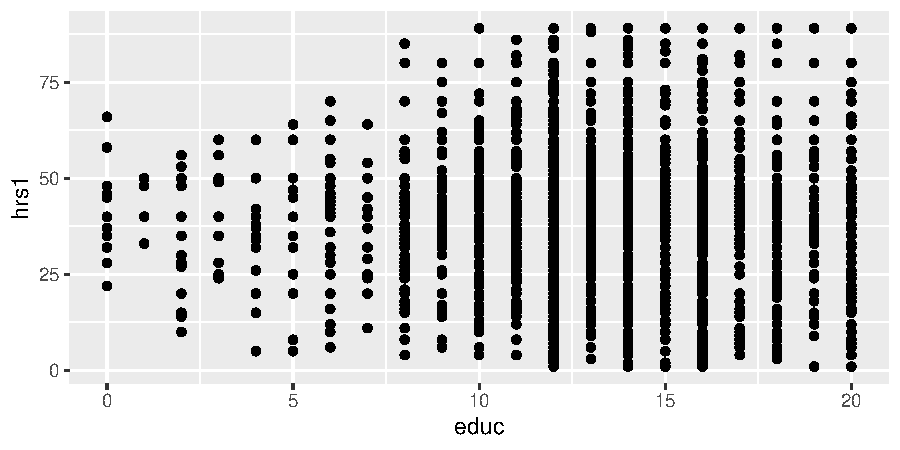
\includegraphics{Kor_BasicStats_files/figure-latex/unnamed-chunk-163-1} \end{center}

이 두 변수 간의 관계가 산포도로는 뚜렷하게 보이지는 않는 것 같습니다. 뭔가 교육시간이 증가할수록 노동시간의 변화가 커지는 거 같기는 한데\ldots{} 그렇다면 둘 간의 `선형' 관계를 포착하기 위해서 선형모델 방법을 이용한 추세선을 그려보겠습니다.

\begin{Shaded}
\begin{Highlighting}[]
\KeywordTok{ggplot}\NormalTok{(}\DataTypeTok{data =}\NormalTok{ GSScut) }\OperatorTok{+}\StringTok{ }
\StringTok{  }\KeywordTok{geom_point}\NormalTok{(}\KeywordTok{aes}\NormalTok{(}\DataTypeTok{x =}\NormalTok{ educ, }\DataTypeTok{y =}\NormalTok{ hrs1)) }\OperatorTok{+}
\StringTok{  }\KeywordTok{geom_smooth}\NormalTok{(}\KeywordTok{aes}\NormalTok{(}\DataTypeTok{x=}\NormalTok{educ, }\DataTypeTok{y=}\NormalTok{hrs1), }\DataTypeTok{method=}\StringTok{'lm'}\NormalTok{)}
\end{Highlighting}
\end{Shaded}

\begin{center}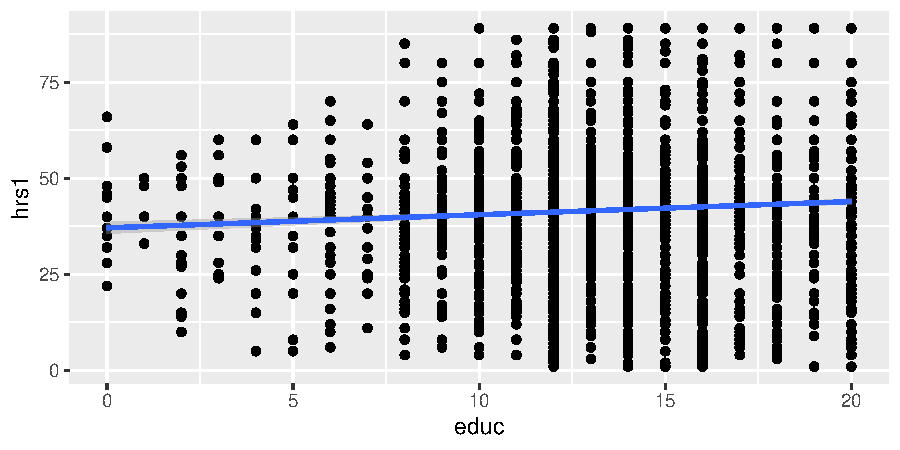
\includegraphics{Kor_BasicStats_files/figure-latex/unnamed-chunk-164-1} \end{center}

플롯을 통해 0.07이라는 크지는 않지만 두 변수 간 양적(positive, +) 상관관계가 존재한다는 것을 확인할 수 있습니다. 즉, 한 변수의 증가가 다른 변수의 증가와 연관이 있다는 것을 의미합니다.

그렇다면 이번에는 노동 시간을 종속변수(dependent variable)로 하고 교육 수준을 설명변수로 하는 단순회귀분석 모델을 만들어보겠습니다. 보통 ``노동 시간에 대한 교육 수준의 단순회귀분석''을 수행한다라고 표현합니다. 이 단순선형회귀 모델은 앞서의 직선을 포함한 플롯과 같은 의미를 가진 결과를 보여줍니다.

\begin{Shaded}
\begin{Highlighting}[]
\NormalTok{model1 <-}\StringTok{ }\KeywordTok{lm}\NormalTok{(hrs1 }\OperatorTok{~}\StringTok{ }\NormalTok{educ, }\DataTypeTok{data =}\NormalTok{ GSScut)}
\NormalTok{model1 }\OperatorTok\StringTok{ }\KeywordTok{summary}\NormalTok{()}
\end{Highlighting}
\end{Shaded}

\begin{verbatim}
## 
## Call:
## lm(formula = hrs1 ~ educ, data = GSScut)
## 
## Residuals:
##     Min      1Q  Median      3Q     Max 
## -42.931  -4.906  -1.196   7.436  48.488 
## 
## Coefficients:
##             Estimate Std. Error t value Pr(>|t|)    
## (Intercept) 37.09273    0.76265  48.636  < 2e-16 ***
## educ         0.34194    0.05375   6.362 2.11e-10 ***
## ---
## Signif. codes:  0 '***' 0.001 '**' 0.01 '*' 0.05 '.' 0.1 ' ' 1
## 
## Residual standard error: 14.33 on 7695 degrees of freedom
##   (5392 observations deleted due to missingness)
## Multiple R-squared:  0.005232,   Adjusted R-squared:  0.005103 
## F-statistic: 40.47 on 1 and 7695 DF,  p-value: 2.109e-10
\end{verbatim}

물론 \textbf{R} 기본 함수로도 더 간단하게 단순선형회귀 모델의 결과를 보여줄 수 있습니다.

\begin{Shaded}
\begin{Highlighting}[]
\KeywordTok{plot}\NormalTok{(}\DataTypeTok{x =}\NormalTok{ GSScut}\OperatorTok{$}\NormalTok{educ, }\DataTypeTok{y =}\NormalTok{ GSScut}\OperatorTok{$}\NormalTok{hrs1)}
\KeywordTok{abline}\NormalTok{(}\KeywordTok{lm}\NormalTok{(model1))}
\end{Highlighting}
\end{Shaded}

\begin{center}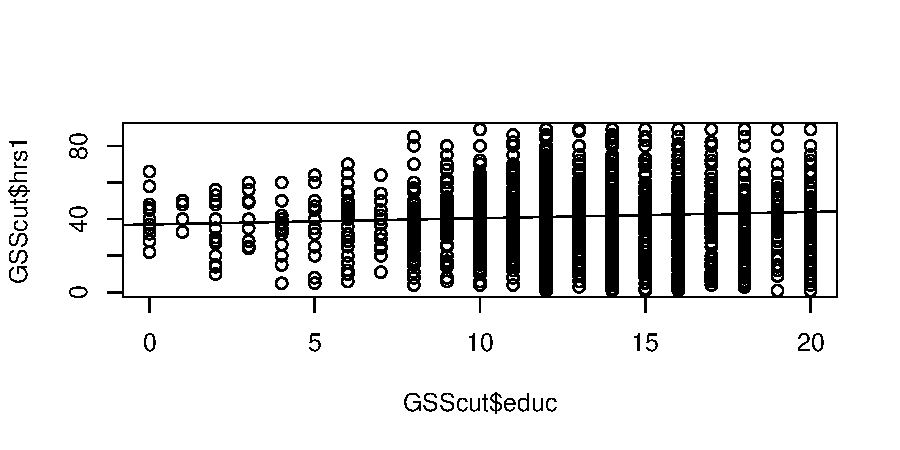
\includegraphics{Kor_BasicStats_files/figure-latex/unnamed-chunk-166-1} \end{center}

하지만 이 플롯의 경우는 단 하나의 설명변수와 종속변수의 관계를 나타날 때만 잘 작동합니다.

회귀분석모델을 이루는 주요 요소는 우리가 설명하고자 하는 종속변수, 그리고 그것을 설명하기 위한 설명변수, 마지막으로 설명하고 남은 나머지---잔차라고 할 수 있습니다.

\begin{itemize}
\item
  간단히 말하면, 잔차는 모델에 적합(fit)되고 남은 나머지를 의미합니다: \texttt{Data\ =\ Fit\ +\ Residual}.
\item
  잔차(\(e_i\))는 관측된 실제의 개별 \(y_i\)와 모델로 예측한 값(\(\hat{y_i}\))의 차이라고 할 수 있습니다: \(e_i = y_i - \hat{y_i}\).
\end{itemize}

따라서 종속변수를 가장 잘 예측하는 선을 그리는 방법 중 하나로 우리는 이 오차들, 잔차의 값을 최대한 작게끔 하는 선을 그리는 방법을 택할 수 있습니다. 그 선을 그리는 데에는 두 가지 방법이 존재합니다.

\begin{itemize}
\item
  첫째, 잔차의 절대값의 총합이 최대한 작아지는 선을 그리는 것
\item
  둘째, 잔차의 제곱합이 최소화되는 선을 그리는 것: 최소자승법(least squares)
\end{itemize}

우리는 이 중에서 둘째, 최소자승법을 사용한 회귀분석을 수행합니다. 왜 최소자승법을 사용할까요? 여기서 자세한 설명을 하기는 어렵지만 수리통계적으로 절대값과 제곱은 모두 값을 양수값으로 변환시켜주는 의미를 지니는 데 반하여(거리의 개념으로 환산. 거리에는 마이너스가 있을 수 없으니까요), 절대값은 계산이 좀 더 수학적으로 복잡하기 때문입니다. 어차피 같은 의미를 지니고 있다면 수리적으로 계산이 편리한 제곱합의 방식을 사용하는 것이 효율적입니다.

이렇게 그려지는 최소자승법에 따른 회귀선은 다음과 같은 공식으로 구현됩니다.

\[ \hat{y} = \beta_0 + \beta_1x\]

\begin{itemize}
\item
  \(\hat{y}\): 모델로 예측한 종속변수 값
\item
  절편: 절편은 회귀곡선과 \(y\)축이 만나는 지점을 의미합니다.

  \begin{itemize}
  \tightlist
  \item
    모집단을 대상으로 기울기의 모수(parameter)는 \(\beta_0\)
  \item
    표본에 대한 점추정치(point estimate)는 \(b_0\)
  \item
    절편은 \(x\)가 0일 때, 기대되는 \(y\)의 값입니다.
  \end{itemize}
\item
  기울기: 회귀분석에서 기울기는 \(b_1 = \frac{s_y}{s_x}r\)로 나타낼 수 있습니다.

  \begin{itemize}
  \tightlist
  \item
    모집단을 대상으로 기울기의 모수는 \(\beta_1\)
  \item
    표본에 대한 점추정치는 \(\beta_1\)
  \item
    기울기는 \(x\)의 한 단위 증가에 따른 \(y\)의 평균적인 증감을 의미합니다.
  \end{itemize}
\item
  \(x\): 설명변수
\end{itemize}

우리는 선형회귀모델을 통하여 주어진 설명변수의 값에 따른 종속변수의 값을 ``예측''(prediction)할 수 있습니다. 공식에 \(x\)값과 주어진 기울기, 절편값을 넣어 계산을 해서 값을 얻어내는 것입니다. 그러나 이러한 예측값은 어디까지나 주어진, 관측된 자료들만으로 구성된 모델로 만들어낸 것이기 때문에 불확실성(uncertainty)가 존재합니다. 그것이 바로 잔차(모집단의 수준에서는 오차)의 존재입니다.

\begin{itemize}
\item
  또 회귀모델에서 고려해야할 것은 외삽의 문제(extrapolation)가 있습니다. 외삽의 문제는 우리에게 주어진 데이터의 값을 벗어난 범주의 값으로 모델을 예측할 때 발생합니다.

  \begin{itemize}
  \tightlist
  \item
    예를 들어, 실제 우리가 가진 관측된 설명변수의 값은 70-100 사이에 분포하는데, 회귀모델로 기울기를 얻을 경우에 우리는 설명변수의 값이 0일때, 20일때, -10일때 등의 종속변수에 대한 예측값을 구할 수 있습니다. 이때, 과연 그러한 예측값은 의미가 있을까요?
  \item
    종종 절편이 외삽의 문제를 직관적으로 보여주고는 합니다.
  \item
    혹은 실제 우리가 관측한 데이터가 사실은 다른 추세의 일부만을 보여주고 있을 때, 주어진 데이터로만 그린 회귀선이 실제의 관계(모집단의 관계)를 전혀 예측하지 못하는 문제가 발생할 수도 있습니다.
  \end{itemize}
\end{itemize}

이번에는 우리가 만든 모델에 대해 잘 만들어졌는지, 종속변수를 기대한대로 설명변수가 잘 설명하고 있는지를 진단(diagnostics)해보겠습니다. 이를 위해서는 최소자승법에 기초한 선형회귀분석의 기본가정들, 조건들에 대해서 살펴볼 필요가 있습니다. 과연 그 조건들이 잘 충족되었는지를 확인해야 우리가 얻은 결과가 충분히 믿을만한 것이라고 볼 수 있기 때문입니다.

회귀분석의 기본가정들은 나중에 \texttt{Lv.2.Statistics} 자료에서 한 번 더 다룰 것이기 때문에, 일단 여기서는 간단하게 설명하도록 하겠습니다.

\begin{itemize}
\item
  선형성(linearity)

  \begin{itemize}
  \tightlist
  \item
    회귀분석을 사용하기 위해서는 두 변수가 선형적인 관계, 한 변수의 증감이 다른 변수의 증감과 연계되어 있을 것이라는 가정이 필요합니다.
  \item
    따라서 선형성을 살펴보기 위해서 앞서 우리가 했던 것처럼 산포도를 그려보고는 합니다.
  \end{itemize}
\item
  잔차의 정규성(Normality of residuals)

  \begin{itemize}
  \item
    한편, 우리는 모집단의 수준에서는 오차(error, \(\epsilon\)), 표본의 수준에서는 잔차(residuals, \(e\))가 정규분포를 띄고 있을 것이라고 가정하며, 이때 오차의 정규분포의 기대값을 0일 것이라고 가정합니다(E(\(\epsilon\)) = 0). 이는 표본의 수준에서는 잔차의 평균이 0일 것이라고 가정한다는 것을 의미합니다.
  \item
    따라서 과연 잔차가 어떻게 생겨먹었는지를 보기 위해서 잔차의 플롯(residual plot)을 그려보겠습니다.

\begin{Shaded}
\begin{Highlighting}[]
\KeywordTok{plot}\NormalTok{(}\DataTypeTok{x =}\NormalTok{ model1}\OperatorTok{$}\NormalTok{fitted.values, }\DataTypeTok{y =}\NormalTok{ model1}\OperatorTok{$}\NormalTok{residuals) }
\KeywordTok{abline}\NormalTok{(}\DecValTok{0}\NormalTok{,}\DecValTok{0}\NormalTok{)}
\end{Highlighting}
\end{Shaded}

    \begin{center}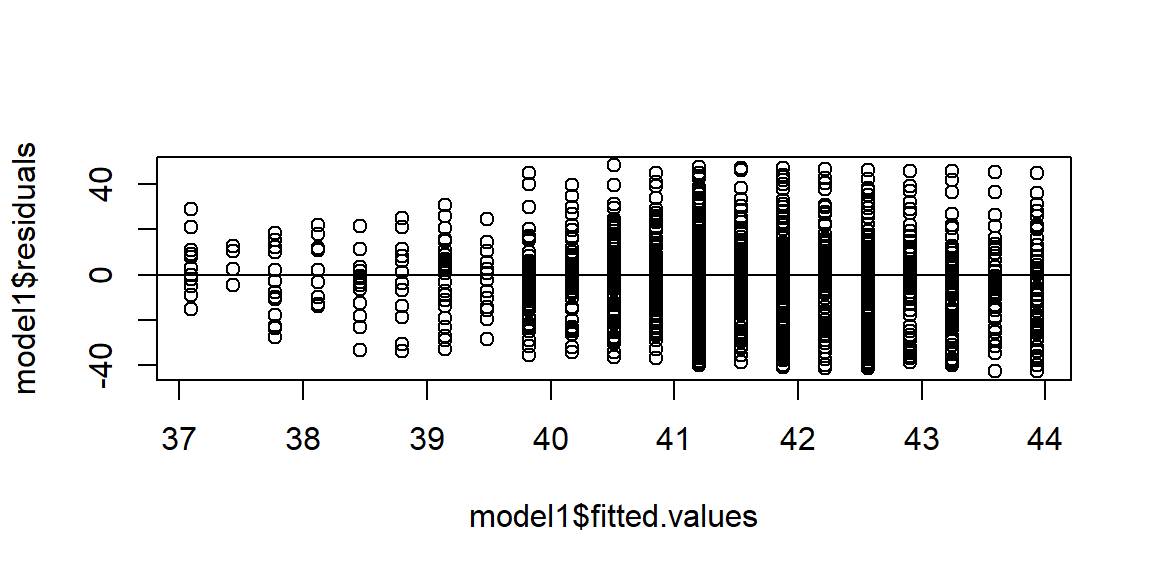
\includegraphics{Kor_BasicStats_files/figure-latex/unnamed-chunk-167-1} \end{center}
  \item
    잔차를 개별 관측치에서 평균과의 차이를 표준편차로 나누어준, 즉 개별 관측치가 평균으로부터 얼마나 떨어져있는지를 보는 표준화된 잔차(standardized residuals)를 보여주겠습니다. 단위(scale)이 달라지는 거지 관계 양상이 변화하는 것은 아닙니다. 반드시 필수적인 것은 아니지만, 어떤 경우에는 유용하게 사용할 수 있습니다.

\begin{Shaded}
\begin{Highlighting}[]
\NormalTok{      stpred1 <-}\StringTok{ }\NormalTok{(model1}\OperatorTok{$}\NormalTok{fitted.values }\OperatorTok{-}\StringTok{ }\KeywordTok{mean}\NormalTok{(model1}\OperatorTok{$}\NormalTok{fitted.values)) }\OperatorTok{/}\StringTok{ }
\StringTok{ }\KeywordTok{sd}\NormalTok{(model1}\OperatorTok{$}\NormalTok{fitted.values)}
\NormalTok{      stres1 <-}\StringTok{ }\NormalTok{(model1}\OperatorTok{$}\NormalTok{residuals }\OperatorTok{-}\StringTok{ }\KeywordTok{mean}\NormalTok{(model1}\OperatorTok{$}\NormalTok{residuals)) }\OperatorTok{/}\StringTok{ }
\StringTok{ }\KeywordTok{sd}\NormalTok{(model1}\OperatorTok{$}\NormalTok{residuals)}
      \KeywordTok{plot}\NormalTok{(}\DataTypeTok{x =}\NormalTok{ stpred1, }\DataTypeTok{y =}\NormalTok{ stres1)}
      \KeywordTok{abline}\NormalTok{(}\DecValTok{0}\NormalTok{,}\DecValTok{0}\NormalTok{)}
\end{Highlighting}
\end{Shaded}

    \begin{center}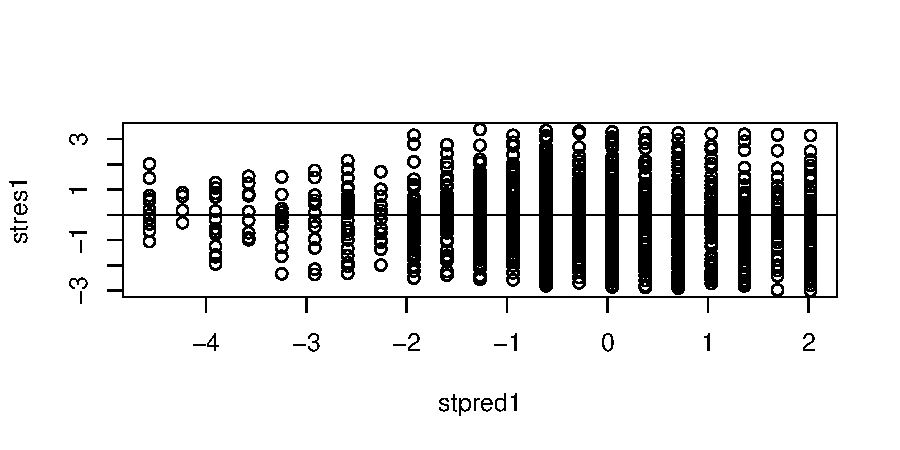
\includegraphics{Kor_BasicStats_files/figure-latex/unnamed-chunk-168-1} \end{center}
  \item
    한편, 잔차의 정규성을 살펴보기 위해서 표준화된 잔차를 정규밀도(normal density)를 통해 히스토그램으로 보여주거나 QQ 플롯으로 보여줄 수 있습니다.

\begin{Shaded}
\begin{Highlighting}[]
\KeywordTok{hist}\NormalTok{(stres1, }\DataTypeTok{freq =} \OtherTok{FALSE}\NormalTok{) }\CommentTok{# 이 히스토그램은 빈도보다는 비율일 때 사용합니다.}
\KeywordTok{curve}\NormalTok{(dnorm, }\DataTypeTok{add =} \OtherTok{TRUE}\NormalTok{)  }\CommentTok{# 이 곡선은 표준화된 잔차에 대해서만 사용가능합니다.}
\end{Highlighting}
\end{Shaded}

    \begin{center}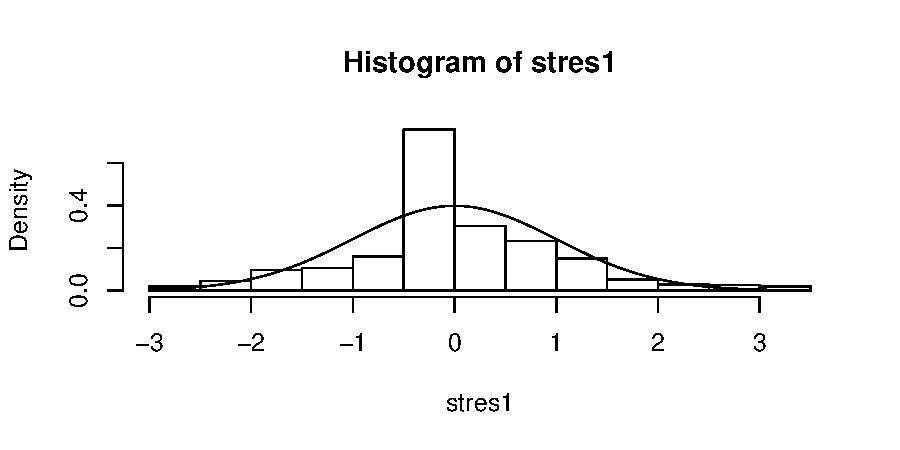
\includegraphics{Kor_BasicStats_files/figure-latex/unnamed-chunk-169-1} \end{center}

\begin{Shaded}
\begin{Highlighting}[]
\KeywordTok{qqnorm}\NormalTok{(stres1)}
\KeywordTok{abline}\NormalTok{(}\DecValTok{0}\NormalTok{,}\DecValTok{1}\NormalTok{)}
\end{Highlighting}
\end{Shaded}

    \begin{center}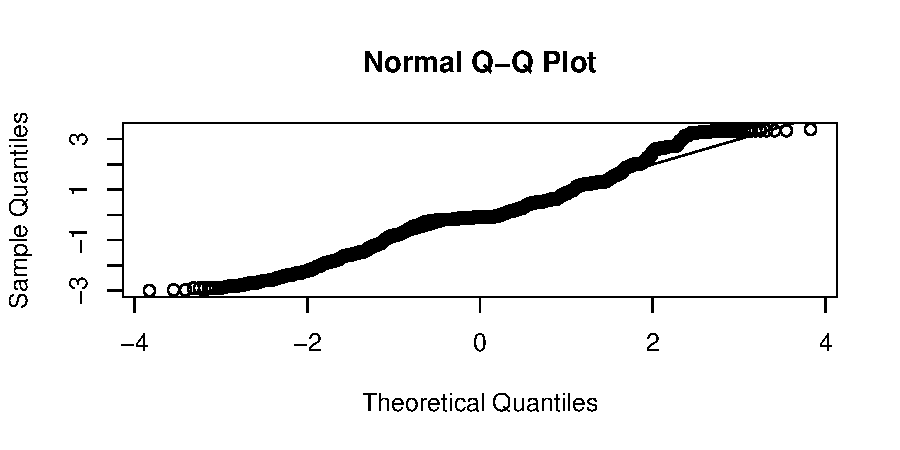
\includegraphics{Kor_BasicStats_files/figure-latex/unnamed-chunk-169-2} \end{center}
  \end{itemize}
\item
  등분산성(constant variance)

  \begin{itemize}
  \item
    최소자승법을 통해 구한 추세선 주변에 개별 관측치들이 일정하게(constant) 분포하여야 한다는 것을 의미합니다.
  \item
    이것은 잔차의 변동성이 0에 수렴해야 한다는 것으로 등분산성(homoskedasticity)이라고도 표현합니다. 위에서와 마찬가지로 QQ 플롯을 통해서 확인해볼 수 있습니다 (45도선에 근사할수록 정규적이라고 볼 수 있습니다).

\begin{Shaded}
\begin{Highlighting}[]
\CommentTok{# install.packages("lmtest") # 등분산성을 검정하기 위한 패키지입니다.}
\KeywordTok{library}\NormalTok{(lmtest)}
\CommentTok{# 등분산성을 검정하기 위해 Breusch-Pagan 검정을 수행하도록 하겠습니다.}
\KeywordTok{bptest}\NormalTok{(model1)}
\end{Highlighting}
\end{Shaded}

\begin{verbatim}
## 
##    studentized Breusch-Pagan test
## 
## data:  model1
## BP = 2.1288, df = 1, p-value = 0.1446
\end{verbatim}
  \item
    브루슈-패건 검정은 등분산성을 검정하기 위한 기법으로, 영가설(\(h_0\))이 오차 간 분산이 일정할 것이다라고 설정한 뒤, 만약 그것이 기각되면(\(p < 0.05\)), 이분산성(heteroskedasticity)의 근거를 얻습니다. 전형적인 통계의 영가설 검정 방식을 취하고 있습니다.
  \item
    만약 우리가 가진 데이터가 영가설을 기각, 이분산성을 가질 것이라고 추정된다면 어떻게 해야할까요? 이때에는 표준오차가 등분산성 가정이 위배됨에 따라 왜곡되었을 것으로 보고, 로버스트 표준오차로 보정하는 작업을 해줍니다.

    \begin{itemize}
    \tightlist
    \item
      이론적 근거는 나중에 \texttt{Lv.2.Statistics}나 \texttt{Lv.3.Statistics}에서 선형확률모형(linear probability models)을 다룰 때 자세하게 언급하도록 하겠습니다.
    \end{itemize}
  \item
    로버스트 표준오차로 보정한 결과를 얻는 작업은 다음과 같은 패키지와 앞에서 로드했던 \texttt{lmtest} 패키지에서 제공하는 코드로 가능합니다.

\begin{Shaded}
\begin{Highlighting}[]
\CommentTok{# install.packages("sandwich")}
\KeywordTok{library}\NormalTok{(sandwich)}
\KeywordTok{coeftest}\NormalTok{(model1, }\DataTypeTok{vcov =} \KeywordTok{vcovHC}\NormalTok{(model1, }\DataTypeTok{type =} \StringTok{"HC1"}\NormalTok{))}
\end{Highlighting}
\end{Shaded}

\begin{verbatim}
## 
## t test of coefficients:
## 
##              Estimate Std. Error t value  Pr(>|t|)    
## (Intercept) 37.092733   0.735076 50.4611 < 2.2e-16 ***
## educ         0.341937   0.052076  6.5661 5.502e-11 ***
## ---
## Signif. codes:  0 '***' 0.001 '**' 0.01 '*' 0.05 '.' 0.1 ' ' 1
\end{verbatim}
  \end{itemize}
\item
  자, 이제는 이탈치(outliers)의 영향력을 살펴보도록 하겠습니다. 이탈치의 영향력을 살펴보는 것은 중요합니다.

  \begin{itemize}
  \tightlist
  \item
    이탈치란 이례적으로(극단적으로) 크거나 작은 값을 지니는 관측치를 의미합니다.

    \begin{itemize}
    \tightlist
    \item
      모델에서 구한 기울기에 큰 영향을 미치는 이탈치를 영향력 있는 관측값(influential points)이라고 부르기도 합니다.
    \end{itemize}
  \item
    왜냐하면 이탈치란 이론적으로는 우리의 일반화를 반증하는 비정상성(abnormality)를 탐지하는 계기가 될 수도 있고,
  \item
    혹은 우리가 일반화하고자 하는 모델의 결과---계수값을 왜곡시키는 요인일 수도 있기 때문입니다.
  \end{itemize}
\item
  두 개의 변수만으로 돌리는 단순회귀분석에서, 예측값(fitted values)과 잔차 간의 관계를 보여주는 플롯은 이탈치를 가시적으로 보여주는 데 유용합니다.

\begin{Shaded}
\begin{Highlighting}[]
\CommentTok{## Cook's distance라는 플롯을 그려보겠습니다.}
\NormalTok{cooksd <-}\StringTok{ }\KeywordTok{cooks.distance}\NormalTok{(model1) }\CommentTok{# 먼저 cooks.distance라는 함수로 앞서 분석한}
\CommentTok{## 단순회귀모델에 기초한 cooksd라는 객체를 만들어줍니다.}
\KeywordTok{plot}\NormalTok{(cooksd, }\DataTypeTok{main=}\StringTok{"Influential Obs by Cooks distance"}\NormalTok{) }\CommentTok{# 보시면 아시겠지만}
\CommentTok{## 이탈치가 모델에 영향을 미쳤는지를 보여주는  플롯입니다.}
\KeywordTok{abline}\NormalTok{(}\DataTypeTok{h =} \DecValTok{1}\NormalTok{, }\DataTypeTok{col=}\StringTok{"red"}\NormalTok{)  }\CommentTok{# 일종의 기준선을 1로 잡아주겠습니다.}
\KeywordTok{text}\NormalTok{(}\DataTypeTok{x=}\DecValTok{1}\OperatorTok{:}\KeywordTok{length}\NormalTok{(cooksd)}\OperatorTok{+}\DecValTok{1}\NormalTok{, }\DataTypeTok{y=}\NormalTok{cooksd, }\DataTypeTok{labels=}\KeywordTok{ifelse}\NormalTok{(cooksd}\OperatorTok{>}\DecValTok{1}\NormalTok{,}\KeywordTok{names}\NormalTok{(cooksd),}\StringTok{""}\NormalTok{),}
     \DataTypeTok{col=}\StringTok{"red"}\NormalTok{)  }\CommentTok{# 1이 넘으면 빨간 색으로 표시하게 지정해주었습니다만,}
\end{Highlighting}
\end{Shaded}

  \begin{center}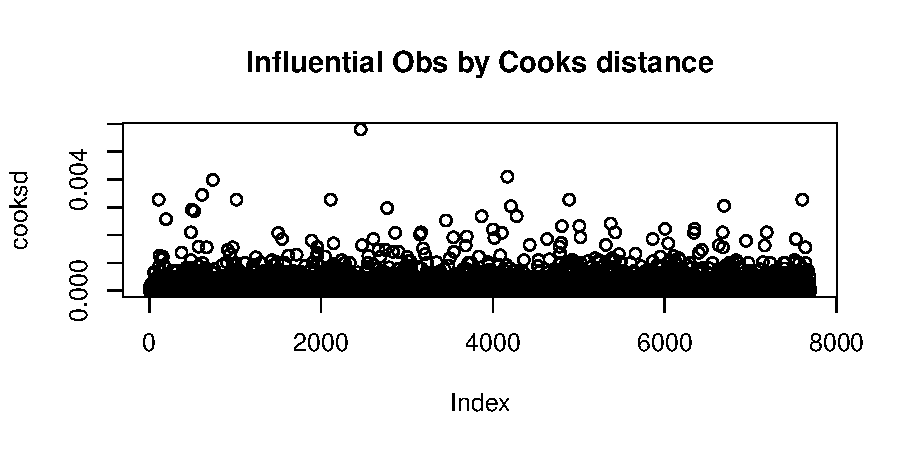
\includegraphics{Kor_BasicStats_files/figure-latex/unnamed-chunk-172-1} \end{center}

\begin{Shaded}
\begin{Highlighting}[]
\CommentTok{## 넘질 않네요. 즉, 이 데이터에서는 이탈치가 별로 없습니다.}
\end{Highlighting}
\end{Shaded}

  \begin{itemize}
  \item
    기술적으로는 Cook's Distance는 모델에서 데이터들을 하나씩 제거해가면서 회귀분석을 반복하여 계산하여 얻어지는데, 이를 통해서 우리는 몇 번째 관측치가 제거되었을 때 회귀모델의 값이 얼만큼 달라지는지 확인할 수 있습니다.

    \begin{itemize}
    \item
      단, 여기에서 1을 Cook's distance의 기준치로 삼은 것은 자의적인 기준입니다. 보통 전체 관측치 수를 기준으로 \(4/n\)을 설정하고는 합니다.

\begin{Shaded}
\begin{Highlighting}[]
\CommentTok{# 다시 Cook's distance 플롯을 그려보겠습니다.}
\KeywordTok{plot}\NormalTok{(cooksd, }\DataTypeTok{main=}\StringTok{"Influential Obs by Cooks distance"}\NormalTok{)  }
\KeywordTok{abline}\NormalTok{(}\DataTypeTok{h =} \DecValTok{4}\OperatorTok{/}\KeywordTok{length}\NormalTok{(cooksd), }\DataTypeTok{col=}\StringTok{"red"}\NormalTok{)}
\KeywordTok{text}\NormalTok{(}\DataTypeTok{x=}\DecValTok{1}\OperatorTok{:}\KeywordTok{length}\NormalTok{(cooksd)}\OperatorTok{+}\DecValTok{1}\NormalTok{, }\DataTypeTok{y=}\NormalTok{cooksd, }
     \DataTypeTok{labels=}\KeywordTok{ifelse}\NormalTok{(cooksd}\OperatorTok{>}\DecValTok{4}\OperatorTok{/}\KeywordTok{length}\NormalTok{(cooksd), }
                   \KeywordTok{names}\NormalTok{(cooksd),}\StringTok{""}\NormalTok{), }\DataTypeTok{col=}\StringTok{"red"}\NormalTok{)}
\end{Highlighting}
\end{Shaded}

      \begin{center}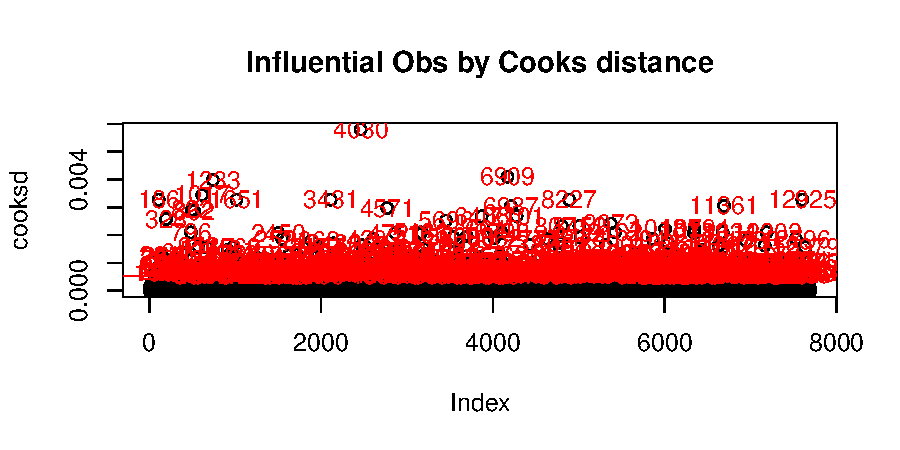
\includegraphics{Kor_BasicStats_files/figure-latex/unnamed-chunk-173-1} \end{center}
    \end{itemize}
  \item
    Cook's distance 플롯을 통해 이탈치를 특정할 수 있게 되면, 그 이탈치들을 제외하고 모델을 다시 돌려볼 수 있습니다.

\begin{Shaded}
\begin{Highlighting}[]
\NormalTok{model1 <-}\StringTok{ }\KeywordTok{lm}\NormalTok{(hrs1 }\OperatorTok{~}\StringTok{ }\NormalTok{educ, }\DataTypeTok{data =}\NormalTok{ GSScut[}\OperatorTok{-}\NormalTok{(}\DecValTok{4030}\NormalTok{),]) }\CommentTok{# 4030번째 관측값 제외}
\end{Highlighting}
\end{Shaded}
  \end{itemize}
\end{itemize}

\hypertarget{uxd68cuxadc0uxbd84uxc11duxc758-uxc774uxd574-uxae30uxc6b8uxae30uxc758-uxac80uxc815}{%
\section{회귀분석의 이해: 기울기의 검정}\label{uxd68cuxadc0uxbd84uxc11duxc758-uxc774uxd574-uxae30uxc6b8uxae30uxc758-uxac80uxc815}}

앞에서는 주로 데이터에 기초하여 통계적 문제들을 짚어보았습니다. 이제는 과연 이렇게 모델을 통해 구한 통계치들이 과연 통계적으로 의미있는 차이를 보여주는 것인지, 혹은 변하는(varying) 값들에 따른 우연에 의한 것인지를 구분하기 위한 검정(testing)에 대해 이론적으로 살펴보고자 합니다.

\begin{itemize}
\item
  먼저 우리가 기울기를 검정하고자 할 때 세우는 가설은 모두 ``모집단''에 대한 것이라는 점을 잊어서는 안 됩니다. 우리가 궁금한 것은 과연 표본 그 너머의 모집단에 존재하는 관계이지, 한정된 표본에서만 관측할 수 있는 관계 양상이 아닙니다.
\item
  앞서 분석한 모델의 단순회귀분석 결과를 다시 불러와 봅시다.

\begin{Shaded}
\begin{Highlighting}[]
\NormalTok{tidy <-}\StringTok{ }\NormalTok{model1 }\OperatorTok\StringTok{ }\NormalTok{broom}\OperatorTok{::}\KeywordTok{tidy}\NormalTok{()}
\NormalTok{tidy }\OperatorTok\StringTok{ }\NormalTok{knitr}\OperatorTok{::}\KeywordTok{kable}\NormalTok{()}
\end{Highlighting}
\end{Shaded}

  \begin{tabular}{l|r|r|r|r}
  \hline
  term & estimate & std.error & statistic & p.value\\
  \hline
  (Intercept) & 37.0105847 & 0.7635843 & 48.469544 & 0\\
  \hline
  educ & 0.3475927 & 0.0538111 & 6.459496 & 0\\
  \hline
  \end{tabular}

  \begin{itemize}
  \item
    여기서 \texttt{statistics}란 t-검정의 결과값으로 우리는 회귀분석의 추론을 검정하기 위해 이 통계치를 사용합니다.

    \begin{itemize}
    \item
      \(\text{t-statistics} = \frac{\text{point estimate} - \text{null value}}{\text{Standard Error}}\)
    \item
      이때, 점추정(point estimate)는 \(b_1\)으로 표본을 통해 우리가 구한, 관측된 기울기를 의미합니다.
    \item
      \(SE_{b1}\)은 관측된 기울기의 표준오차를 의미합니다.\footnote{표준오차의 개념이 조금 헷갈릴 수 있습니다. 간단하게 설명하자면, 우리가 하나의 표본을 가지로 기울기, 절편 등을 구하지만 그것이 결코 모집단의 것과 같다고 우리는 확신할 수 없습니다. 왜냐하면 모집단에서 수많은 표본들을 뽑을 수 있지만 현실의 제약으로 우리는 단 하나만을 뽑아서 그것의 결과를 확인한 것이기 때문입니다. 따라서 이론적으로는 백만개의 표본을 뽑을 수 있다고 하면, 우리는 백만개의 기울기, 절편을 얻을 수 있을 것입니다. 이때, 이 백만개의 기울기와 절편도 분포의 형태로 나타낼 수 있을 텐데, 그 기울기와 절편들의 분포의 표준편차를 표준오차라고 부릅니다. 즉, 본질적으로 오차가 존재할 수밖에 없는 표집(sampling)의 변동성을 포착하는 통계치라고 할 수 있습니다.}
    \item
      기울기와 관련된 자유도(degree of freedom)는 표본의 규모에서 변수와 절편을 제외한 \(n-2\) 입니다.
    \end{itemize}
  \end{itemize}
\end{itemize}

따라서 주어진 값들로 t값을 계산해보면,

\begin{itemize}
\item
  대략적으로 \(\text{t-statistics} = \frac{0.3419 - 0}{0.0537} = 6.3668\) 정도라고 할 수 있습니다. 오차는 소수점 때문입니다. 간략하게 보여주기 위해서 소수점 넷째자리에서 끊었기 때문에 결과가 조금 다릅니다.
\item
  자유도는 7,695개 관측치에서 둘을 빼준 7,693이므로,
\item
  통계적 유의수준(p-value)는 \(P(|T| > 6.3668) < 0.05\)로 통계적으로 유의하다는 것을 확인할 수 있습니다. 사실 아마 0.0001 보다 작다 뭐 이정도이지 않을까 싶습니다.
\end{itemize}

통계적으로 계수값이 우연의 결과가 아니라 실제 설명변수에 의한 것일 확률이 높다는 것을 보여주기 위해서 계수값의 표준오차를 이용한 변동 구간이 0, 즉 효과없음(null effect, null value)을 포함하고 있는지 살펴볼 수도 있습니다. 그 변동구간을 우리는 신뢰구간이라고 합니다. 신뢰구간은 기울기값과 그 기울기값에 대한 t-값에 표준오차를 곱한 범위를 보여줍니다. 이 모델에서 신뢰구간은 다음과 같이 나타내줄 수 있습니다.

\[ \text{Confidence Intervals} = b_1 \pm t^{*}_{\text{df} = n-2} \times SE_{b_1}\]
+ 이때, 효과없음을 0으로 설정하는 것은 설명변수와 종속변수 간의 어떠한 관계도 없다는 것을 보여주기 위함입니다.

\begin{itemize}
\item
  회귀분석 결과로 주어지는 \(b_1, SE_{b_1}\)는 양측꼬리 검정(two-tailed)으로 계산된 p-value 값을 보여줍니다. 즉, 기울기의 영가설은 0이라는 것을 의미합니다.
\item
  주로 변수들 간의 관계에 주목하기 때문에 절편에 대한 추론은 거의 하지 않습니다.
\end{itemize}

\hypertarget{uxc880-uxb354-uxbcf5uxc7a1uxd55c-uxd68cuxadc0uxbd84uxc11duxc758-uxc774uxd574-uxb2e4uxbcc0uxb7c9-uxd68cuxadc0uxbd84uxc11d-multivariate-regressionuxc5d0-uxb4e4uxc5b4uxc11cuxae30}{%
\section{좀 더 복잡한 회귀분석의 이해: 다변량 회귀분석 (multivariate regression)에 들어서기}\label{uxc880-uxb354-uxbcf5uxc7a1uxd55c-uxd68cuxadc0uxbd84uxc11duxc758-uxc774uxd574-uxb2e4uxbcc0uxb7c9-uxd68cuxadc0uxbd84uxc11d-multivariate-regressionuxc5d0-uxb4e4uxc5b4uxc11cuxae30}}

만약 우리가 남성과 여성이 노동 시간에 대해서 서로 다른 기준치를 가지고 있다고 가정한다면 어떻게 될까요? 즉, 이는 수리통계적으로는 남성과 여성이 서로 다른 절편값(intercepts)를 가지고 있다는 것을 의미하며, 실질적으로는 다른 어떠한 변수의 영향력에서 자유로울 때, 종속변수에서 남성과 여성이 차이가 있을 것이라는 것을 의미합니다. 그렇다면 두 번째 모델을 한 번 만들어보겠습니다.

\begin{Shaded}
\begin{Highlighting}[]
\NormalTok{model2 <-}\StringTok{ }\KeywordTok{lm}\NormalTok{(hrs1 }\OperatorTok{~}\StringTok{ }\NormalTok{educ }\OperatorTok{+}\StringTok{ }\NormalTok{female, }\DataTypeTok{data =}\NormalTok{ GSScut)}
\KeywordTok{summary}\NormalTok{(model2)}
\end{Highlighting}
\end{Shaded}

\begin{verbatim}
## 
## Call:
## lm(formula = hrs1 ~ educ + female, data = GSScut)
## 
## Residuals:
##     Min      1Q  Median      3Q     Max 
## -46.204  -5.661   0.390   5.881  50.933 
## 
## Coefficients:
##             Estimate Std. Error t value Pr(>|t|)    
## (Intercept) 33.44023    0.77008  43.424  < 2e-16 ***
## educ         0.38560    0.05259   7.332  2.5e-13 ***
## female       6.05139    0.31958  18.935  < 2e-16 ***
## ---
## Signif. codes:  0 '***' 0.001 '**' 0.01 '*' 0.05 '.' 0.1 ' ' 1
## 
## Residual standard error: 14.01 on 7694 degrees of freedom
##   (5392 observations deleted due to missingness)
## Multiple R-squared:  0.04952,    Adjusted R-squared:  0.04928 
## F-statistic: 200.4 on 2 and 7694 DF,  p-value: < 2.2e-16
\end{verbatim}

앞서의 단순회귀분석에서 산포도에 회귀선 하나를 포함할 때와는 달리, 서로 다른 두 개의 선을 그려주고자 할 때는 모델에서 서로 다른 변수 각각의 계수값을 벡터로 추출해서 사용해야 합니다.

\begin{Shaded}
\begin{Highlighting}[]
\NormalTok{model2}\OperatorTok{$}\NormalTok{coefficients}
\end{Highlighting}
\end{Shaded}

\begin{verbatim}
## (Intercept)        educ      female 
##  33.4402284   0.3856016   6.0513934
\end{verbatim}

\begin{Shaded}
\begin{Highlighting}[]
\KeywordTok{plot}\NormalTok{(}\DataTypeTok{x =}\NormalTok{ GSScut}\OperatorTok{$}\NormalTok{educ, }\DataTypeTok{y =}\NormalTok{ GSScut}\OperatorTok{$}\NormalTok{hrs1)}
 \KeywordTok{abline}\NormalTok{(model2}\OperatorTok{$}\NormalTok{coefficients[}\DecValTok{1}\NormalTok{], model2}\OperatorTok{$}\NormalTok{coefficients[}\DecValTok{2}\NormalTok{] ) }\CommentTok{# 남성일 경우의 회귀선}
 \KeywordTok{abline}\NormalTok{((model2}\OperatorTok{$}\NormalTok{coefficients[}\DecValTok{1}\NormalTok{] }\OperatorTok{+}\StringTok{ }
\StringTok{           }\NormalTok{model2}\OperatorTok{$}\NormalTok{coefficients[}\DecValTok{3}\NormalTok{]), model2}\OperatorTok{$}\NormalTok{coefficients[}\DecValTok{2}\NormalTok{] ) }\CommentTok{# 여성일 경우의 회귀선}
\end{Highlighting}
\end{Shaded}

\begin{center}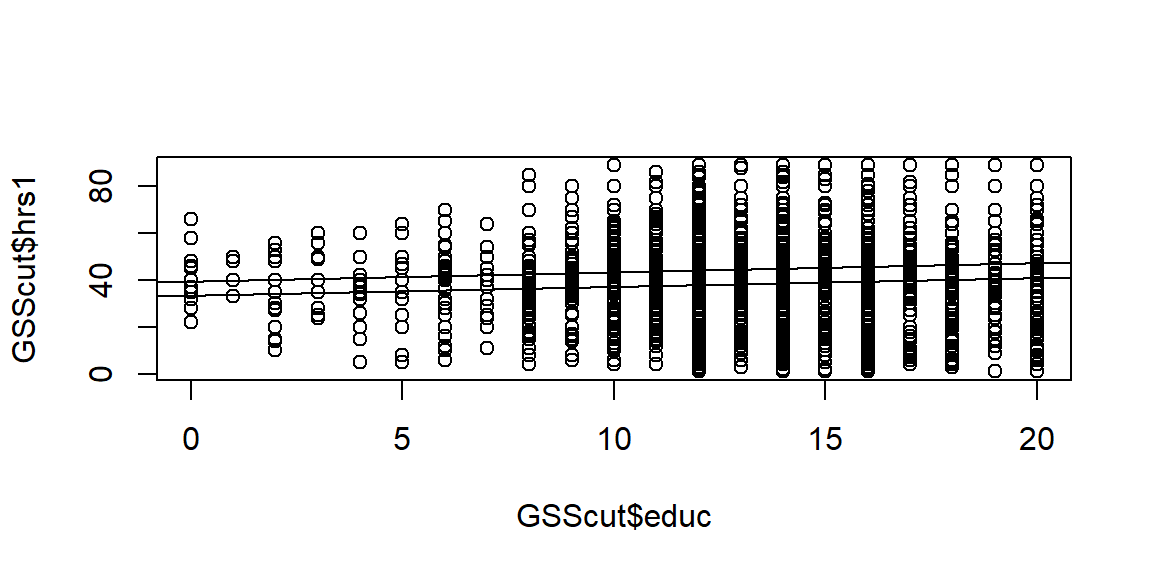
\includegraphics{Kor_BasicStats_files/figure-latex/unnamed-chunk-177-1} \end{center}

사실 식으로 보면 까다롭지는 않습니다. 모델 2는 \(\text{Worked Hours} = \beta_0 + \beta_1(\text{Education}) + \beta_2(\text{Female}) + \epsilon\) 이라고 할 수 있습니다. 이때, 여성일 경우, 이 모델 2의 추정치는 \(\text{Worked Hours} = \beta_0 + \beta_1(\text{Education}) + \beta_2 \times 1 + \epsilon\), 남성일 경우는 \(\text{Worked Hours} = \beta_0 + \beta_1(\text{Education}) + \beta_2 \times 0 + \epsilon\)입니다. 선형회귀분석에서 기울기를 구하는 방법 중 하나는 편미분(partial derivatives, \(\partial\))을 하는 것입니다.

\begin{itemize}
\item
  여성일 경우: \(\frac{\partial(\text{Worked Hours})}{\partial(\text{Female})} = \beta_0 + \beta_2\)로 절편을 구할 수 있습니다.
\item
  반면, 남성일 경우: \(\frac{\partial(\text{Worked Hours})}{\partial(\text{Male})} = \beta_0\)이 됩니다. 남성의 대표값은 0이기 때문입니다.
\item
  이때, 두 회귀선은 평행(parellel)한 기울기를 가집니다. 절편값(\((\beta_0 + \beta_2) - \beta_0 = \beta_2\)만 달라지는 것입니다.
\end{itemize}

모델 2는 성별에 따라서 교육 연수의 효과가 동일할 것(비조건적일 것)이라고 가정하지만 여성의 경우 남성일 때와는 다른 기준치를 가진다고 봅니다.

그렇다면 만약 남성과 여성일 때 각각 서로 다른 기울기를 갖는다고, 즉 교육 연수가 성별에 따라 서로 다른 효과를 가진다고 생각해보면 어떻게 될까요? 선형모델 함수와 \texttt{ggplot2} 패키지를 이용해서 한 번 그려보겠습니다.

\begin{Shaded}
\begin{Highlighting}[]
\KeywordTok{ggplot}\NormalTok{(}\DataTypeTok{data =}\NormalTok{ GSScut) }\OperatorTok{+}\StringTok{ }
\StringTok{  }\KeywordTok{geom_point}\NormalTok{(}\KeywordTok{aes}\NormalTok{(}\DataTypeTok{x =}\NormalTok{ educ, }\DataTypeTok{y =}\NormalTok{ hrs1, }\DataTypeTok{color =} \KeywordTok{as.factor}\NormalTok{(female))) }\OperatorTok{+}\StringTok{ }
\StringTok{  }\KeywordTok{geom_smooth}\NormalTok{(}\KeywordTok{aes}\NormalTok{(}\DataTypeTok{x =}\NormalTok{ educ, }\DataTypeTok{y =}\NormalTok{ hrs1, }\DataTypeTok{color =} \KeywordTok{as.factor}\NormalTok{(female)), }\DataTypeTok{method =} \StringTok{"lm"}\NormalTok{)}
\end{Highlighting}
\end{Shaded}

\begin{center}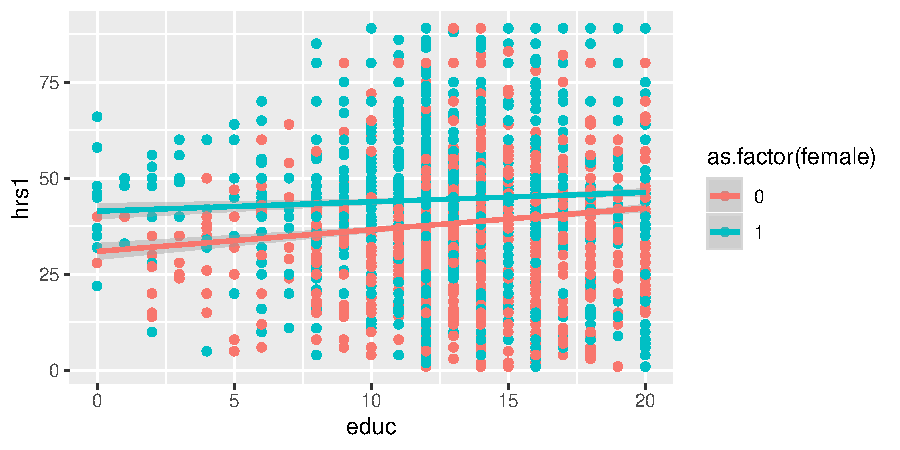
\includegraphics{Kor_BasicStats_files/figure-latex/unnamed-chunk-178-1} \end{center}

위의 플롯은 교육 연수가 노동 시간에 미치는 효과가 성별에 따라 ``조건적''일 것이라는 것을 가정하고 분석한 것이다. 회귀식으로 모델을 재구성하면 다음과 같다.

\begin{Shaded}
\begin{Highlighting}[]
\NormalTok{model3 <-}\StringTok{ }\KeywordTok{lm}\NormalTok{(hrs1 }\OperatorTok{~}\StringTok{ }\NormalTok{educ }\OperatorTok{*}\StringTok{ }\NormalTok{female, }\DataTypeTok{data =}\NormalTok{ GSScut) }
\KeywordTok{summary}\NormalTok{(model3)}
\end{Highlighting}
\end{Shaded}

\begin{verbatim}
## 
## Call:
## lm(formula = hrs1 ~ educ * female, data = GSScut)
## 
## Residuals:
##     Min      1Q  Median      3Q     Max 
## -45.319  -5.341   0.035   5.663  51.286 
## 
## Coefficients:
##             Estimate Std. Error t value Pr(>|t|)    
## (Intercept) 30.95939    1.12811  27.444  < 2e-16 ***
## educ         0.56288    0.07897   7.128 1.11e-12 ***
## female      10.46820    1.50271   6.966 3.52e-12 ***
## educ:female -0.31830    0.10582  -3.008  0.00264 ** 
## ---
## Signif. codes:  0 '***' 0.001 '**' 0.01 '*' 0.05 '.' 0.1 ' ' 1
## 
## Residual standard error: 14 on 7693 degrees of freedom
##   (5392 observations deleted due to missingness)
## Multiple R-squared:  0.05064,    Adjusted R-squared:  0.05027 
## F-statistic: 136.8 on 3 and 7693 DF,  p-value: < 2.2e-16
\end{verbatim}

이와 같이 두 설명변수 간의 상호작용항(interaction terms)는 설명변수 간 종속변수에 대한 조건적 효과를 분석하는 데 도움을 주지만, 해석에 주의를 요합니다.

\begin{itemize}
\item
  다음과 같은 회귀모델을 가정해봅시다: \(\text{Worked Hours} = \beta_0 + \beta_1(\text{Education}) + \beta_2(\text{Female}) + \beta_3(\text{Education} \times \text{Female}) + \epsilon\).
\item
  이때, 한계효과(marginal effects)는 설명변수 \(x_i\)에 대한 기울기(\(\beta_i\))의 도함수로 나타낼 수 있습니다. 아까 위에서 간략하게 살펴본 편미분을 의미합니다.

  \begin{itemize}
  \item
    교육 연수의 한계효과 = \(\beta_1 + \text{Female} \times \beta_3\)
  \item
    여성의 한계효과 = \(\beta_2 + \text{Education} \times \beta_3\)
  \item
    남성일 때(\texttt{Female\ =\ 0}) 기울기와 절편은 \(\beta_1\)과 \(\beta_0\)으로 나타낼 수 있습니다. 여성일 때(\texttt{Female\ =\ 1})의 기울기와 절편은 \(\beta_1 + \beta_3\)과 \(\beta_0 + \beta_2\)로 나타낼 수 있습니다.
  \end{itemize}
\item
  모델 3의 계수값을 분석해보겠습니다.

\begin{Shaded}
\begin{Highlighting}[]
\NormalTok{model3}\OperatorTok{$}\NormalTok{coefficients}
\end{Highlighting}
\end{Shaded}

\begin{verbatim}
## (Intercept)        educ      female educ:female 
##  30.9593917   0.5628771  10.4681951  -0.3183006
\end{verbatim}

\begin{Shaded}
\begin{Highlighting}[]
\KeywordTok{plot}\NormalTok{(}\DataTypeTok{x =}\NormalTok{ GSScut}\OperatorTok{$}\NormalTok{educ, }\DataTypeTok{y =}\NormalTok{ GSScut}\OperatorTok{$}\NormalTok{hrs1)}
\CommentTok{## abline 함수는 abline(절편값, 기울기값)으로 설정해줄 수 있습니다;}
\KeywordTok{abline}\NormalTok{(model3}\OperatorTok{$}\NormalTok{coefficients[}\DecValTok{1}\NormalTok{], model3}\OperatorTok{$}\NormalTok{coefficients[}\DecValTok{2}\NormalTok{])}
\KeywordTok{abline}\NormalTok{((model3}\OperatorTok{$}\NormalTok{coefficients[}\DecValTok{1}\NormalTok{] }\OperatorTok{+}\StringTok{ }\NormalTok{model3}\OperatorTok{$}\NormalTok{coefficients[}\DecValTok{3}\NormalTok{]), }
\NormalTok{       (model3}\OperatorTok{$}\NormalTok{coefficients[}\DecValTok{2}\NormalTok{] }\OperatorTok{+}\StringTok{ }\NormalTok{model3}\OperatorTok{$}\NormalTok{coefficients[}\DecValTok{4}\NormalTok{]))}
\end{Highlighting}
\end{Shaded}

  \begin{center}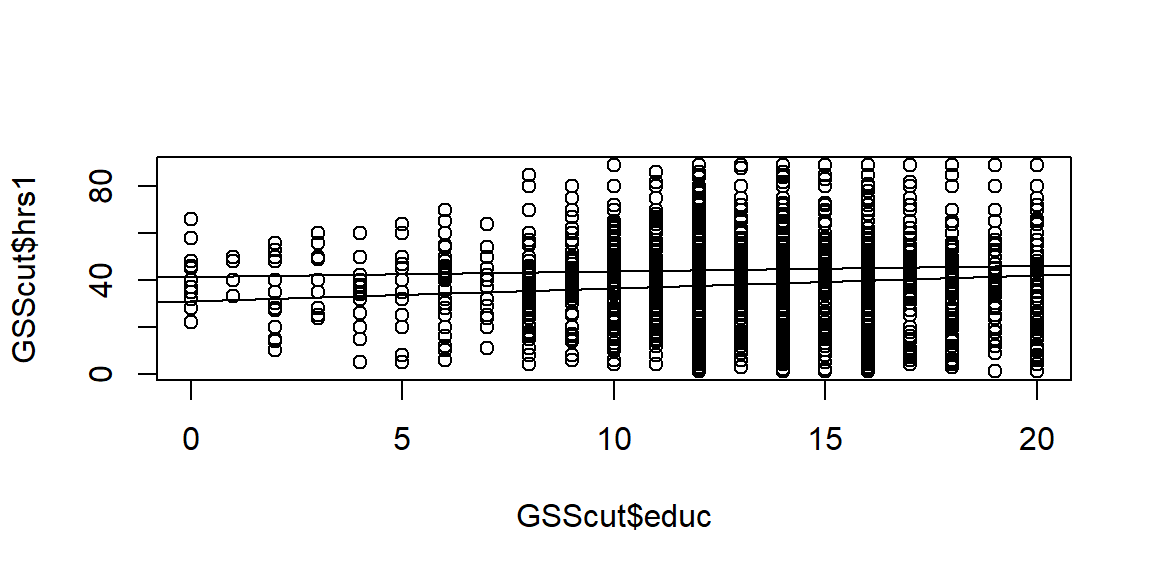
\includegraphics{Kor_BasicStats_files/figure-latex/unnamed-chunk-181-1} \end{center}
\end{itemize}

교육 연수가 0일 때, 남성과 여성의 노동 시간의 차이는 얼마일까요? 교육 연수가 20일 때는 어떤 차이가 나타날까요? 교육 연수가 증가할수록 성별의 효과가 평준화된다고 가정하는 것이 맞을까요? 아니면 교육 연수와 성별, 노동 시간에 영향을 미치는 다른 변수들이 존재할까요? 잠재적인 탈허위적 상관관계(spurious correlations)에 대해 생각해볼 필요가 있습니다.

\hypertarget{uxb2e8uxc21cuxd68cuxadc0uxbd84uxc11d-uxc2ecuxd654}{%
\section{단순회귀분석 심화}\label{uxb2e8uxc21cuxd68cuxadc0uxbd84uxc11d-uxc2ecuxd654}}

이번에는 \texttt{Quality\ of\ Government} 데이터셋의 교차사례 데이터를 이용해 단순회귀분석을 수행, 그 결과표가 보여주는 개별 통계치들의 의미를 살펴보겠습니다. 단, 심화의 이론적 배경 등은 나중에 \texttt{Lv.2.Statistics}에서 자세하게 논의할 것입니다. 여기에서는 \textbf{R}의 기본 함수들로도 원리를 이해하면 패키지 없이 해당 통계치들을 계산해낼 수 있다는 것을 보여주고가 합니다.

\begin{Shaded}
\begin{Highlighting}[]
\NormalTok{QOG <-}\StringTok{ }\KeywordTok{pick}\NormalTok{(}\DataTypeTok{file =} \StringTok{"http://www.qogdata.pol.gu.se/data/qog_std_cs_jan19.dta"}\NormalTok{)}
\end{Highlighting}
\end{Shaded}

예제 데이터 \texttt{QOG}는 194개 국가의 2015년을 기준으로 약 1983개의 변수들을 포함하고 있는 변수입니다. 우리는 이 중에서 부패지수(\texttt{ti\_cpi})와 세계화 지수(\texttt{dr\_ig})를 사용하여 단순회귀분석을 수행할 것입니다. 먼저, \texttt{QOG}에서 필요한 변수만을 선택하여 서브셋을 만들어보겠습니다.

\begin{Shaded}
\begin{Highlighting}[]
\NormalTok{QOGcut <-}\StringTok{ }\NormalTok{QOG }\OperatorTok\StringTok{ }\KeywordTok{select}\NormalTok{(ccodecow, cname, ti_cpi, dr_ig)}
\end{Highlighting}
\end{Shaded}

서브셋, \texttt{QOGcut}에서 사용할 변수들의 간략한 기술통계(descriptive statistics)를 살펴보도록 하겠습니다.

\begin{Shaded}
\begin{Highlighting}[]
\NormalTok{QOGcut }\OperatorTok\StringTok{ }\KeywordTok{select}\NormalTok{(ti_cpi, dr_ig) }\OperatorTok\StringTok{ }\KeywordTok{summary}\NormalTok{() }\OperatorTok\StringTok{ }\NormalTok{knitr}\OperatorTok{::}\KeywordTok{kable}\NormalTok{()}
\end{Highlighting}
\end{Shaded}

\begin{tabular}{l|l|l}
\hline
  &     ti\_cpi &     dr\_ig\\
\hline
 & Min.   : 8.00 & Min.   :28.68\\
\hline
 & 1st Qu.:28.00 & 1st Qu.:50.49\\
\hline
 & Median :38.00 & Median :59.93\\
\hline
 & Mean   :42.97 & Mean   :61.13\\
\hline
 & 3rd Qu.:55.75 & 3rd Qu.:70.90\\
\hline
 & Max.   :91.00 & Max.   :90.47\\
\hline
 & NA's   :16 & NA's   :10\\
\hline
\end{tabular}

현재 부패지수는 최대값이 100으로, 높을수록 '청렴하다는 것'을 의미합니다. 따라서 더 큰 값이 더 높은 수준의 부패를 보여주도록 다시 코딩해보도록 하겠습니다.

\begin{Shaded}
\begin{Highlighting}[]
\NormalTok{QOGcut <-}\StringTok{ }\NormalTok{QOGcut }\OperatorTok\StringTok{ }\KeywordTok{mutate}\NormalTok{(}
  \DataTypeTok{corrupt =} \DecValTok{100} \OperatorTok{-}\StringTok{ }\NormalTok{ti_cpi}
\NormalTok{)}
\end{Highlighting}
\end{Shaded}

이렇게 다시 코딩한 부패지수(\texttt{corrupt})를 포함하여 모델 분석에 사용할 변수들을 다시 한 번 살펴보겠습니다.

\begin{Shaded}
\begin{Highlighting}[]
\NormalTok{QOGcut }\OperatorTok\StringTok{ }\KeywordTok{select}\NormalTok{(corrupt, dr_ig) }\OperatorTok\StringTok{ }\KeywordTok{summary}\NormalTok{() }\OperatorTok\StringTok{ }\NormalTok{knitr}\OperatorTok{::}\KeywordTok{kable}\NormalTok{()}
\end{Highlighting}
\end{Shaded}

\begin{tabular}{l|l|l}
\hline
  &    corrupt &     dr\_ig\\
\hline
 & Min.   : 9.00 & Min.   :28.68\\
\hline
 & 1st Qu.:44.25 & 1st Qu.:50.49\\
\hline
 & Median :62.00 & Median :59.93\\
\hline
 & Mean   :57.03 & Mean   :61.13\\
\hline
 & 3rd Qu.:72.00 & 3rd Qu.:70.90\\
\hline
 & Max.   :92.00 & Max.   :90.47\\
\hline
 & NA's   :16 & NA's   :10\\
\hline
\end{tabular}

세계화 지수를 종속변수로, 부패지수를 설명변수로 하는 단순회귀분석을 수행해보겠습니다.

\begin{Shaded}
\begin{Highlighting}[]
\NormalTok{model0 <-}\StringTok{ }\KeywordTok{lm}\NormalTok{(dr_ig }\OperatorTok{~}\StringTok{ }\NormalTok{corrupt, }\DataTypeTok{data =}\NormalTok{ QOGcut) }
\KeywordTok{summary}\NormalTok{(model0)}
\end{Highlighting}
\end{Shaded}

\begin{verbatim}
## 
## Call:
## lm(formula = dr_ig ~ corrupt, data = QOGcut)
## 
## Residuals:
##     Min      1Q  Median      3Q     Max 
## -32.831  -6.497   0.015   6.788  20.030 
## 
## Coefficients:
##             Estimate Std. Error t value Pr(>|t|)    
## (Intercept) 92.90546    2.19976   42.23   <2e-16 ***
## corrupt     -0.54974    0.03676  -14.96   <2e-16 ***
## ---
## Signif. codes:  0 '***' 0.001 '**' 0.01 '*' 0.05 '.' 0.1 ' ' 1
## 
## Residual standard error: 9.458 on 172 degrees of freedom
##   (20 observations deleted due to missingness)
## Multiple R-squared:  0.5653, Adjusted R-squared:  0.5628 
## F-statistic: 223.7 on 1 and 172 DF,  p-value: < 2.2e-16
\end{verbatim}

이같은 결과는 \textbf{R}에서 제공되는 패키지 이외에도 수리통계적 식을 매뉴얼대로 구성하여 재현할 수도 있습니다. 먼저, 관측치 중 변수에서 결측치가 있으면 해당 관측치 전체는 회귀모형에서 제외됩니다. 새로운 데이터셋(\texttt{temp.data})로 수리통계적 재현을 수행해보도록 하겠습니다.

\begin{Shaded}
\begin{Highlighting}[]
\NormalTok{temp.data <-}\StringTok{ }\NormalTok{QOGcut }\OperatorTok\StringTok{ }\KeywordTok{drop_na}\NormalTok{() }\CommentTok{# 결측치를 제외시켜줍니다.}
\end{Highlighting}
\end{Shaded}

결측치가 존재하지 않는 새로운 데이터셋의 변수들로 OLS 회귀분석의 계수들을 구해보겠습니다. 우리가 추정하고자 하는 회귀식은 \(\text{Index of Globalization} = \beta_0 + \beta_1(\text{Corrupt Index}) + \epsilon\)이라고 할 수 있습니다.

\begin{Shaded}
\begin{Highlighting}[]
\NormalTok{y <-}\StringTok{ }\NormalTok{temp.data}\OperatorTok{$}\NormalTok{dr_ig   }\CommentTok{# 종속변수: 세계화 지수}
\NormalTok{x <-}\StringTok{ }\NormalTok{temp.data}\OperatorTok{$}\NormalTok{corrupt }\CommentTok{# 설명변수: 역전시킨(reversed) 부패 지수}
\end{Highlighting}
\end{Shaded}

그리고 회귀식에서 기울기를 구하는 공식인 \(\beta_1 = \frac{\sigma_y}{\sigma_x} \times cov(y, x)\)라고 할 때,

\begin{Shaded}
\begin{Highlighting}[]
\NormalTok{b1 <-}\StringTok{ }\NormalTok{(}\KeywordTok{sd}\NormalTok{(y) }\OperatorTok{/}\StringTok{ }\KeywordTok{sd}\NormalTok{(x)) }\OperatorTok{*}\StringTok{ }\KeywordTok{cor}\NormalTok{(y, x)}
\NormalTok{b0 <-}\StringTok{ }\KeywordTok{mean}\NormalTok{(y) }\OperatorTok{-}\StringTok{ }\NormalTok{b1 }\OperatorTok{*}\StringTok{ }\KeywordTok{mean}\NormalTok{(x)}
\end{Highlighting}
\end{Shaded}

라고 표현할 수 있습니다. 표본 자료를 사용하여 컴파일하는 것이기 때문에 \(\beta\)가 아니라 표본의 통계치인 \(b\)로 객체를 저장해주었습니다.

OLS는 행렬대수의 형태, \((X'X)^{-1}X'y)\)로 나타낼 수 있습니다. 이렇게 만들어진 \(x\)의 벡터의 맨 앞에 1일 더하여 절편을 나타냅니다. 다른 행렬값들은 변수에 따라 달라지지만, 절편은 상수(constant), 변하지 않는 값이기 때문입니다.

\begin{Shaded}
\begin{Highlighting}[]
\NormalTok{x.matrix <-}\StringTok{ }\KeywordTok{as.matrix}\NormalTok{(}\KeywordTok{cbind}\NormalTok{(}\KeywordTok{rep}\NormalTok{(}\DecValTok{1}\NormalTok{, }\KeywordTok{nrow}\NormalTok{(temp.data)), x))}
\end{Highlighting}
\end{Shaded}

이 \(x\)의 행렬을 이용하여 우리는 기울기의 벡터값을 얻을 수 있습니다.

\begin{Shaded}
\begin{Highlighting}[]
\NormalTok{b.vector <-}\StringTok{ }\KeywordTok{solve}\NormalTok{(}\KeywordTok{t}\NormalTok{(x.matrix) }\OperatorTok\StringTok{ }\NormalTok{x.matrix) }\OperatorTok\StringTok{ }\NormalTok{(}\KeywordTok{t}\NormalTok{(x.matrix) }\OperatorTok\StringTok{ }\NormalTok{y)}
\end{Highlighting}
\end{Shaded}

기울기와 절편을 구했으니, 주어진 \(x\)값과 기울기, 절편을 이용하여 종속변수의 예측값(predicted values, fitted values)을 구할 수도 있습니다. 예측값은 \(\hat{y}\)으로 나타냅니다.\footnote{참고로 평균은 \(\bar{y}\)로 나타냅니다.}

\begin{Shaded}
\begin{Highlighting}[]
\NormalTok{y.hat <-}\StringTok{ }\NormalTok{b0 }\OperatorTok{+}\StringTok{ }\NormalTok{b1 }\OperatorTok{*}\StringTok{ }\NormalTok{x}
\end{Highlighting}
\end{Shaded}

예측값을 구했으니, 과연 예측값과 실제값이 얼마나 차이나는지 플롯을 그려보겠습니다.

\begin{Shaded}
\begin{Highlighting}[]
\KeywordTok{plot}\NormalTok{(y.hat, y)}
\KeywordTok{abline}\NormalTok{(}\DecValTok{0}\NormalTok{, }\DecValTok{1}\NormalTok{)}
\end{Highlighting}
\end{Shaded}

\begin{center}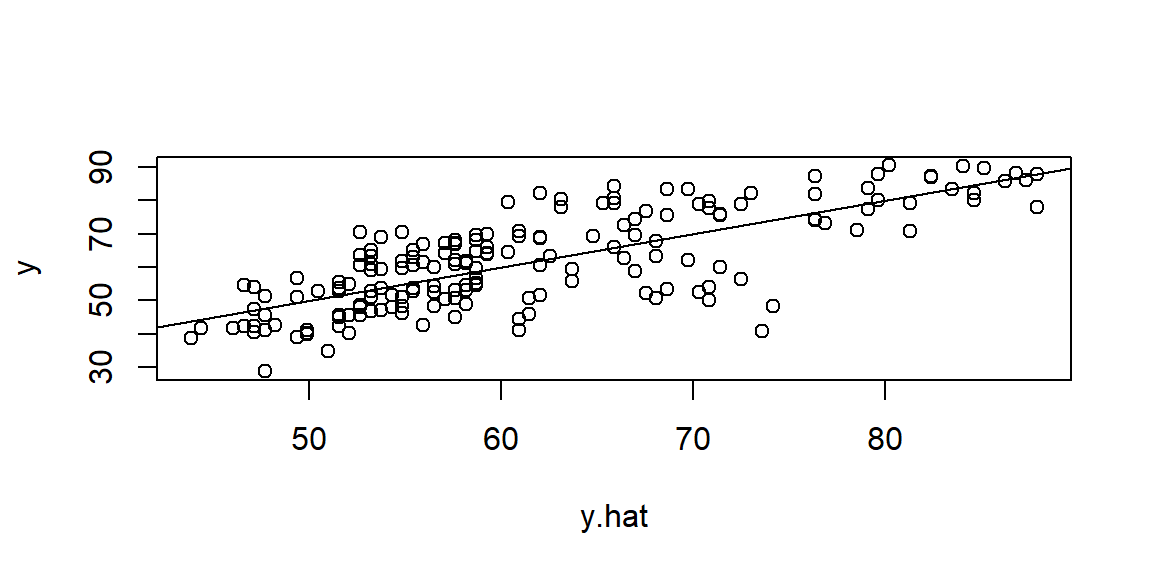
\includegraphics{Kor_BasicStats_files/figure-latex/unnamed-chunk-194-1} \end{center}

예측값과 실제값 간의 차이, 오차를 우리는 표본 수준에서 잔차(residuals)라고 한다고 앞에서 이미 언급한 바가 있습니다. 잔차를 구해보겠습니다.

\begin{Shaded}
\begin{Highlighting}[]
\NormalTok{resid <-}\StringTok{ }\NormalTok{y }\OperatorTok{-}\StringTok{ }\NormalTok{y.hat}
\end{Highlighting}
\end{Shaded}

과연 이 잔차는 회귀분석의 가정에 따라 평균이 0인 정규분포를 이루고 있을까요? 혹은, 이에 근사할까요?

\begin{Shaded}
\begin{Highlighting}[]
\KeywordTok{hist}\NormalTok{(resid)}
\end{Highlighting}
\end{Shaded}

\begin{center}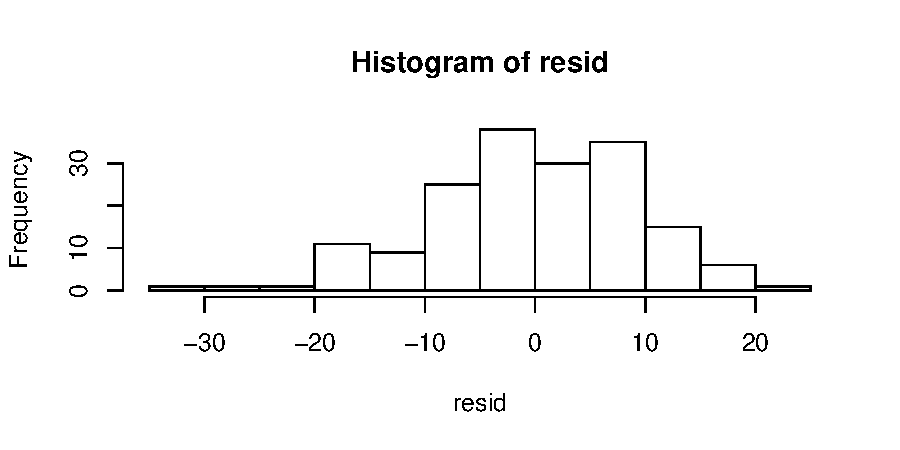
\includegraphics{Kor_BasicStats_files/figure-latex/unnamed-chunk-196-1} \end{center}

\begin{Shaded}
\begin{Highlighting}[]
\KeywordTok{mean}\NormalTok{(resid)}
\end{Highlighting}
\end{Shaded}

\begin{verbatim}
## [1] 7.812197e-16
\end{verbatim}

또 다른 가정에 따르면 잔차는 설명변수와 종속변수에에 독립적이어야 합니다. 과연 이 모델에서 잔차와 설명변수, 잔차와 종속변수는 상관성이 있을까요?

\begin{Shaded}
\begin{Highlighting}[]
\KeywordTok{cor}\NormalTok{(}\KeywordTok{cbind}\NormalTok{(resid, x))}
\end{Highlighting}
\end{Shaded}

\begin{verbatim}
##             resid           x
## resid 1.00000e+00 1.43717e-16
## x     1.43717e-16 1.00000e+00
\end{verbatim}

\begin{Shaded}
\begin{Highlighting}[]
\KeywordTok{par}\NormalTok{(}\DataTypeTok{mfrow =} \KeywordTok{c}\NormalTok{(}\DecValTok{1}\NormalTok{, }\DecValTok{2}\NormalTok{))}
\KeywordTok{plot}\NormalTok{(x, resid)}
\KeywordTok{plot}\NormalTok{(y.hat, resid)}
\end{Highlighting}
\end{Shaded}

\begin{center}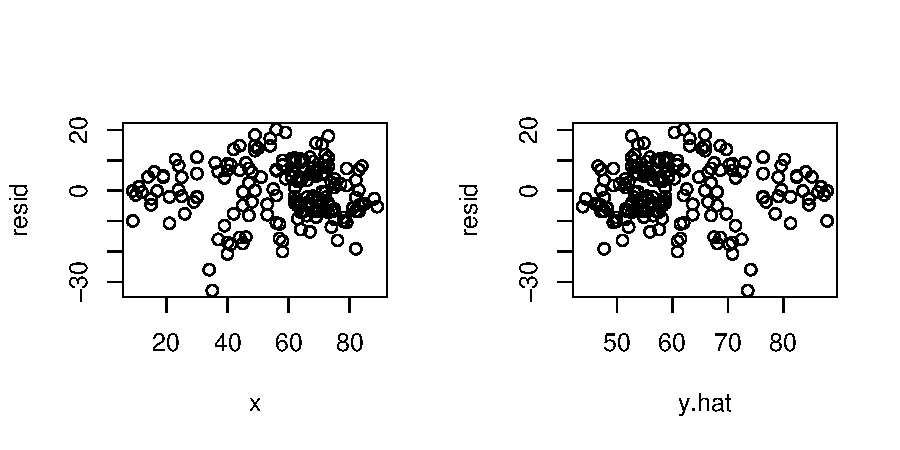
\includegraphics{Kor_BasicStats_files/figure-latex/unnamed-chunk-197-1} \end{center}

플롯을 보면 잔차는 모델에 포함된 변수들과는 큰 상관성을 보이지 않는 것 같습니다. 그렇다면 이번에는 모델의 설명력을 보여주는 \(R^2\) 값을 계산해보도록 하겠습니다. \(R^2\)는 두 가지 방식으로 계산할 수 있습니다. \(R^2\)는 전체 종속변수의 변동량(total sum of squares) 중 설명이 되는 변동량(explained sum of squared)이 차지하는 비율을 보여줍니다.

\begin{itemize}
\item
  첫째, 단순회귀분석에서는 말 그대로 상관계수, \(R\)을 제곱하여 구할 수 있습니다.

\begin{Shaded}
\begin{Highlighting}[]
\KeywordTok{cor}\NormalTok{(y, x)}\OperatorTok{^}\DecValTok{2}
\end{Highlighting}
\end{Shaded}

\begin{verbatim}
## [1] 0.5697705
\end{verbatim}
\item
  둘째, 회귀선을 통해 설명하는 것이 아무 정보도 없을 때 평균을 통해 예측하는 것에 비하여 얼마나 더 나은 설명력을 제공하는지로 보여줄 수 있습니다.

\begin{Shaded}
\begin{Highlighting}[]
\NormalTok{SSE <-}\StringTok{ }\KeywordTok{sum}\NormalTok{((y.hat }\OperatorTok{-}\StringTok{ }\KeywordTok{mean}\NormalTok{(y))}\OperatorTok{^}\DecValTok{2}\NormalTok{) }\CommentTok{# 예측값과 평균값의 차이의 제곱합}
\NormalTok{SSR <-}\StringTok{ }\KeywordTok{sum}\NormalTok{((y }\OperatorTok{-}\StringTok{ }\NormalTok{y.hat)}\OperatorTok{^}\DecValTok{2}\NormalTok{) }\CommentTok{# 실제값과 예측값의 차이의 제곱합(잔차의 제곱합)}
\NormalTok{R2 <-}\StringTok{ }\NormalTok{SSE }\OperatorTok{/}\StringTok{ }\NormalTok{(SSE }\OperatorTok{+}\StringTok{ }\NormalTok{SSR) }\CommentTok{# 모델로 예측했을 때와 평균으로 예측했을 때의 차이를}
                        \CommentTok{## 전체 변동량 대비 비율로 표현합니다.}
\NormalTok{R2}
\end{Highlighting}
\end{Shaded}

\begin{verbatim}
## [1] 0.5697705
\end{verbatim}

  \begin{itemize}
  \item
    \(R^2\)는 변수의 개수에 따라 조정됩니다. 왜냐하면 어떠한 변수든 간에 통계적으로 모델에 추가되면, \(R^2\)는 증가하기 때문입니다. 따라서 우리는 과연 그것이 유의미한 변수의 추가로 인한 모델의 설명력 증가인지, 단순히 변수 추가투입에 따른 \(R^2\) 증가인지 살펴보기 위해 조정된 \(R^2\)를 구하고는 합니다.
  \item
    조정된 \(R^2\)는 \(\frac{n-1}{n-k}\)로 가중치가 부여됩니다.

\begin{Shaded}
\begin{Highlighting}[]
\NormalTok{n <-}\StringTok{ }\KeywordTok{length}\NormalTok{(y)}
\NormalTok{k <-}\StringTok{ }\DecValTok{1}
\NormalTok{adj.R2 <-}\StringTok{ }\DecValTok{1} \OperatorTok{-}\StringTok{ }\NormalTok{(((}\DecValTok{1} \OperatorTok{-}\StringTok{ }\NormalTok{R2) }\OperatorTok{*}\StringTok{ }\NormalTok{(n }\OperatorTok{-}\StringTok{ }\DecValTok{1}\NormalTok{)) }\OperatorTok{/}\StringTok{ }\NormalTok{(n }\OperatorTok{-}\StringTok{ }\NormalTok{k }\OperatorTok{-}\StringTok{ }\DecValTok{1}\NormalTok{))}
\end{Highlighting}
\end{Shaded}

    모델을 통해 예측하는 것이 평균(대표값)이나 다른 방법으로 추세를 예측하는 것에 비해 더 많은 정보를 준다는 것을 보여주는 또 하나의 통계치는 F-검정치입니다. 마찬가지로 설명되지 않은 변동량에 비해 설명된 변동량을 보여주는 통계치입니다. 수리통계적으로는 잔차의 제곱합(\(SSR / (n-k)\)에 대한 모델로 설명되는 변동량의 제곱합(\(SSE / k\))으로 계산할 수 있습니다.
  \end{itemize}
\end{itemize}

\begin{Shaded}
\begin{Highlighting}[]
\NormalTok{dfm <-}\StringTok{ }\NormalTok{k}
\NormalTok{dfr <-}\StringTok{ }\NormalTok{n }\OperatorTok{-}\StringTok{ }\NormalTok{k }\OperatorTok{-}\StringTok{ }\DecValTok{1}

\NormalTok{MSM <-}\StringTok{ }\NormalTok{SSE}\OperatorTok{/}\NormalTok{dfm}
\NormalTok{MSR <-}\StringTok{ }\NormalTok{SSR}\OperatorTok{/}\NormalTok{dfr }
\NormalTok{F <-}\StringTok{ }\NormalTok{MSM }\OperatorTok{/}\StringTok{ }\NormalTok{MSR}
\end{Highlighting}
\end{Shaded}

이렇게 구한 F값이 과연 통계적으로 유의미한지, 유의수준을 계산해보도록 하겠습니다.

\begin{Shaded}
\begin{Highlighting}[]
\DecValTok{1} \OperatorTok{-}\StringTok{ }\KeywordTok{pf}\NormalTok{(F, dfm, dfr) }\CommentTok{# 거의 0에 수렴합니다. F값은 통계적으로 유의미하다는}
\end{Highlighting}
\end{Shaded}

\begin{verbatim}
## [1] 0
\end{verbatim}

\begin{Shaded}
\begin{Highlighting}[]
                    \CommentTok{# 근거가 된다고 할 수 있습니다.}
\end{Highlighting}
\end{Shaded}

잔차의 표준편차와 종속변수의 표준편차를 비교해보겠습니다. 잔차의 표준편차는 모델로 설명되고 남은 나머지 변동량을 보여주며, 종속변수의 표준편차는 설명변수로 설명되기 이전의 종속변수의 변동량을 보여줍니다. 설명변수가 종속변수의 변이를 설명하여 잔차의 표준편차가 감소한 것을 확인할 수 있습니다.

\begin{Shaded}
\begin{Highlighting}[]
\KeywordTok{sqrt}\NormalTok{(MSR) }
\end{Highlighting}
\end{Shaded}

\begin{verbatim}
## [1] 9.411872
\end{verbatim}

\begin{Shaded}
\begin{Highlighting}[]
\KeywordTok{sd}\NormalTok{(y)}
\end{Highlighting}
\end{Shaded}

\begin{verbatim}
## [1] 14.30737
\end{verbatim}

이제는 각 계수값에 대한 t검정을 수행해보도록 하겠습니다 먼저 1이 포함된 \(x\), 설명변수 행렬을 이용하여 공분산행렬(variance-covariance matrix)을 계산합니다.

\begin{Shaded}
\begin{Highlighting}[]
\NormalTok{vcov <-}\StringTok{ }\DecValTok{1} \OperatorTok{/}\StringTok{ }\NormalTok{(n }\OperatorTok{-}\StringTok{ }\NormalTok{k }\OperatorTok{-}\StringTok{ }\DecValTok{1}\NormalTok{) }\OperatorTok{*}\StringTok{ }\KeywordTok{as.numeric}\NormalTok{(}\KeywordTok{t}\NormalTok{(resid) }\OperatorTok\StringTok{ }\NormalTok{resid) }\OperatorTok{*}\StringTok{ }
\StringTok{  }\KeywordTok{solve}\NormalTok{(}\KeywordTok{t}\NormalTok{(x.matrix) }\OperatorTok\StringTok{ }\NormalTok{x.matrix)}
\NormalTok{vcov}
\end{Highlighting}
\end{Shaded}

\begin{verbatim}
##                          x
##    4.79281101 -0.075692250
## x -0.07569225  0.001338385
\end{verbatim}

각 계수값의 표준오차는 이 공분산의 제곱근으로 계산할 수 있습니다.

\begin{Shaded}
\begin{Highlighting}[]
\NormalTok{SE.b0 <-}\StringTok{ }\KeywordTok{sqrt}\NormalTok{(vcov[}\DecValTok{1}\NormalTok{,}\DecValTok{1}\NormalTok{])}
\NormalTok{SE.b1 <-}\StringTok{ }\KeywordTok{sqrt}\NormalTok{(vcov[}\DecValTok{2}\NormalTok{,}\DecValTok{2}\NormalTok{])}
\CommentTok{## 이제 계수값에 대한 t검정을 수행해보겠습니다.}
\NormalTok{t.b0 <-}\StringTok{ }\NormalTok{(b0 }\OperatorTok{-}\StringTok{ }\DecValTok{0}\NormalTok{) }\OperatorTok{/}\StringTok{ }\NormalTok{SE.b0}
\DecValTok{1} \OperatorTok{-}\StringTok{ }\KeywordTok{pt}\NormalTok{(t.b0, }\DataTypeTok{df =}\NormalTok{ n }\OperatorTok{-}\StringTok{ }\NormalTok{k }\OperatorTok{-}\StringTok{ }\DecValTok{1}\NormalTok{)}
\end{Highlighting}
\end{Shaded}

\begin{verbatim}
## [1] 0
\end{verbatim}

\begin{Shaded}
\begin{Highlighting}[]
\NormalTok{t.b1 <-}\StringTok{ }\NormalTok{(b1 }\OperatorTok{-}\StringTok{ }\DecValTok{0}\NormalTok{) }\OperatorTok{/}\StringTok{ }\NormalTok{SE.b1}
\KeywordTok{pt}\NormalTok{(t.b1, }\DataTypeTok{df =}\NormalTok{ n }\OperatorTok{-}\StringTok{ }\NormalTok{k }\OperatorTok{-}\StringTok{ }\DecValTok{1}\NormalTok{)}
\end{Highlighting}
\end{Shaded}

\begin{verbatim}
## [1] 1.929361e-33
\end{verbatim}

t검정의 의미는 간단합니다. 우리가 모델을 통해 구한 기울기가 과연 실제 설명변수의 효과로 인한 것인지 아니면 단지 설명변수의 변동에 의한 우연의 일치인지를 구분하고자 하는 것입니다.

이렇게 구한 결과를 \texttt{lm()} 함수의 결과와 비교해보겠습니다.

\begin{Shaded}
\begin{Highlighting}[]
\KeywordTok{summary}\NormalTok{(model0)}
\end{Highlighting}
\end{Shaded}

\begin{verbatim}
## 
## Call:
## lm(formula = dr_ig ~ corrupt, data = QOGcut)
## 
## Residuals:
##     Min      1Q  Median      3Q     Max 
## -32.831  -6.497   0.015   6.788  20.030 
## 
## Coefficients:
##             Estimate Std. Error t value Pr(>|t|)    
## (Intercept) 92.90546    2.19976   42.23   <2e-16 ***
## corrupt     -0.54974    0.03676  -14.96   <2e-16 ***
## ---
## Signif. codes:  0 '***' 0.001 '**' 0.01 '*' 0.05 '.' 0.1 ' ' 1
## 
## Residual standard error: 9.458 on 172 degrees of freedom
##   (20 observations deleted due to missingness)
## Multiple R-squared:  0.5653, Adjusted R-squared:  0.5628 
## F-statistic: 223.7 on 1 and 172 DF,  p-value: < 2.2e-16
\end{verbatim}

\begin{Shaded}
\begin{Highlighting}[]
\NormalTok{manual <-}\StringTok{ }\KeywordTok{as_tibble}\NormalTok{(}\KeywordTok{bind_cols}\NormalTok{(}
  \DataTypeTok{Term =} \KeywordTok{c}\NormalTok{(}\StringTok{"(Intercept)"}\NormalTok{, }\StringTok{"Corrupt"}\NormalTok{),}
  \DataTypeTok{Estimate =} \KeywordTok{c}\NormalTok{(b0, b1),}
  \DataTypeTok{Std.Error =} \KeywordTok{c}\NormalTok{(SE.b0, SE.b1),}
  \DataTypeTok{R.sq =} \KeywordTok{c}\NormalTok{(R2, }\OtherTok{NA}\NormalTok{),}
  \DataTypeTok{F =} \KeywordTok{c}\NormalTok{(F, }\OtherTok{NA}\NormalTok{)))}
\NormalTok{manual }\OperatorTok\StringTok{ }\NormalTok{knitr}\OperatorTok{::}\KeywordTok{kable}\NormalTok{()}
\end{Highlighting}
\end{Shaded}

\begin{tabular}{l|r|r|r|r}
\hline
Term & Estimate & Std.Error & R.sq & F\\
\hline
(Intercept) & 92.8618773 & 2.1892490 & 0.5697705 & 226.4623\\
\hline
Corrupt & -0.5505395 & 0.0365839 & NA & NA\\
\hline
\end{tabular}

거의 유사한 결과를 얻을 수 있습니다. 약간의 차이는 \textbf{R} 내부에서 계산할 때 사용되는 공식의 미세한 수리적 차이 때문이라고 이해하실 수 있을 것 같습니다.

\hypertarget{better-understanding-for-linear-model}{%
\chapter{Better Understanding for Linear Model}\label{better-understanding-for-linear-model}}

제6장에서 단순선형회귀모델(simple linear regression model)에 대한 기본적인 내용들을 주로 \textbf{R}코드와 통계치들을 중심으로 살펴보았다면, 이 장에서는 설명변수가 2개 이상인 다중선형회귀모델(multiple linear regression model)로 나아가기 이전에 짚고 넘어가야할 선형모델에 대한 이론적 배경들을 짚어보고자 합니다.

이론적인 측면에서 제4장과 제5장에서 이어진다고 할 수 있습니다. 구체적으로 이 장은 추정(estimation)-유의성 검정(significance tests)-선형회귀모델과 상관관계 순으로 앞선 장들에서 놓치고 넘어갈 수 있었던 이론적인 논의들을 다루어보고자 합니다.

\hypertarget{uxcd94uxc815estimation}{%
\section{추정(Estimation)}\label{uxcd94uxc815estimation}}

첫 번째 절에서는 추정의 문제를 살펴볼 것입니다. 통계방법을 이용하여 우리는 무엇을 추정하려고 하는 것인지, 그리고 추정에는 어떠한 종류가 있는지, 데이터에 따라 우리가 추정해야하기 위해 주목해야하는 것이 무엇인지 등을 다룹니다.

\hypertarget{uxc810uxcd94uxc815uxacfc-uxad6cuxac04uxcd94uxc815point-estimation-and-interval-estimation}{%
\subsection{점추정과 구간추정(point estimation and interval estimation)}\label{uxc810uxcd94uxc815uxacfc-uxad6cuxac04uxcd94uxc815point-estimation-and-interval-estimation}}

무엇인가를 추정한다는 것은 표본과 모집단의 관계로 설명할 수 있습니다. 현실세계 속에서 우리가 사회현상에 대한 모집단을 관측한다는 것은 불가능에 가깝습니다. 따라서 우리는 관측가능한 자료, 표본(sample) 데이터를 통하여 모집단의 모수(parameters)의 값을 ``추정''하고자 합니다. 즉, 추정의 목적은 본질적으로는 표본을 통하여 모집단의 특성을 이해하는 것에 있습니다. 이 지점에서 제5장에서 살펴보았던 ``추론''의 개념이 등장합니다. 모집단을 확보할 수 없으니, 모집단을 잘 대표할 것이라고 기대되는 그 일부, 표본을 통해 모집단이 이러이러할 것이다---라는 추론(inference)을 하게 되는 것이지요.

정량적 변수들을 이용해서 우리는 모집단의 평균(mean)을 추정할 수 있으며, 명목형 변수-분류형 변수를 이용해서는 각 부류가 전체 분류에서 차지하는 비율(proportion)을 추정할 수 있습니다.

통계학에서는 여러 가지 유사한 용어들이 나오고, 그것들을 구분하여 사용하는 것이 중요합니다. 예를 들어, 지금 언급하고 있는 추정(estimation)과 추정량(estimator)은 서로 다른 개념입니다.

\begin{itemize}
\item
  추정량(estimator)이란 표본의 비율(sample proportion), 표본의 평균(saple mean)과 같은 모집단의 모수를 추정하기 위한 특정한 통계치(statistic)을 의미합니다.
\item
  이때 통계치(statistic)은 모집단의 모수(parameter)와 대칭적 관계로 이해할 수 있으며, 표본의 통계적 특성을 의미한다고 볼 수 있습니다.
\item
  한편, 추정값(estimate)은 표본의 특정한 값을 지칭합니다. 예를 들어, 표본의 비율(estimator)의 값(estimate)이 0.73이라는 식으로 표현할 수 있습니다.
\end{itemize}

모든 추정이 동일하지는 않습니다. 왜냐하면 우리는 모집단을 알지 못하여 표본을 가지고 모집단의 특성을 추정, 추론하기 때문에 우리의 추정에는 불확실성(uncertainty)이 존재하는 탓입니다. 여기서는 점추정량(point estimate)과 구간추정량(interval estimate)을 살펴보고자 합니다.

\begin{itemize}
\item
  점추정량이란 모수의 값(parameter value)에 대해 최선의 추측이라고 할 수 있는 단 하나의 통계치(single statistic value)를 의미합니다. 즉, 표본을 통해 모집단의 평균이 0.5일 것이라고 말할 때, 우리는 그 0.5를 점추정량이라고 말할 수 있습니다.
\item
  반면, 구간추정량은 점추정량 둘러싼 구간을 의미하는데, 모수값을 포함할 것이라고 기대되는 ``고정된 신뢰수준''(fixed confidence level)을 보여주는 구간\footnote{유의성 검정 부분에서 한 번 더 짚고 넘어갈 것이지만, 여기에서 의미하는 신뢰수준이란 표본과 모집단, 그리고 표집(sampling)의 문제와 관련이 있습니다. 우리가 얻는 특정한 추정량들은 표집 방법에 따라 충분히 표본이 모집단에 대해 대표성을 가진다고 할 때, 신뢰할 수 있는 결과로 받아들여집니다. 그럼에도 불구하고, 모집단에서 표본을 뽑아낸다는 본연적 한계로 인하여 우리는 표본에서 얻어낸 결과가 모집단을 제대로 보여주지 못했을 결과를 감안해야만 합니다. 신뢰구간이란 이론적으로 총 몇 번의 표집과정을 되풀이했을 때, 그 중 얼마만큼의 잘못된 추정을 가질 확률을 의미합니다. 예를 들어, 100번의 표집을 거쳐 5번의 다른 결과를 얻었을 때, 우리는 95\%의 확률로 그 결과값을 신뢰할 수 있다고 보는 것입니다.}이라고 할 수 있습니다. 이 점에서 우리는 이 구간추정량에 대해 신뢰구간(confidence interval)이라고 합니다.
\end{itemize}

추정, 추정량, 추정값을 이해하는 것은 아마도 모집단의 모수를 제대로, 잘 추정하는 추정량을 얻기 위해서일 것입니다. 그렇다면 좋은 추정량은 무엇일까요? 크게 두 가지 기준을 생각해볼 수 있습니다.

첫째는 불편성(unbiasness)입니다. 이는 추정량의 표집분포가 모집단 값을 중심으로 분포되어 있어야 한다는 것을 의미합니다. 즉, 추정량은 표본을 바탕으로 한 것이기 때문에 모수를 추정하는 데 있어서 불확실성을 내표할수밖에 없지만, 그 불확실성이 모수를 중심으로 퍼져있는 것이라면 우리는 기대값---평균이나 비율 등을 이용하여 모수를 추정할 수 있습니다. 만약 추정량이 편향되어 있다면(biased), 평균적으로 모수를 과소추정(underestimate)하거나 과대추정(overestimate)한다면 우리는 그 결과를 신뢰하기 어려울 것입니다.

두 번째로는 효율성(efficiency)이 있습니다. 가능한 한 작은 표준오차를 통하여 추정할수록 우리는 그 추정량이 다른 추정량에 비하여 모수를 평균적으로 더 `가깝게' 추정하는 효율적인 추정량일 것이라고 기대하게 됩니다. 표준오차가 크다는 것은 그만큼 불확실하다는 것이고 우리가 모수값을 추정하는 데 믿기 어려운 결과라는 의미입니다. 그렇다면 우리는 그 불확실성을 보정하기 위하여 추가적인 조치들을 취해야할 것이고, 그 결과는 비효율적(inefficient)이라고 할 수 있습니다.

동시에 신뢰구간의 문제도 함께 생각해볼 필요가 있습니다. 신뢰구간은 앞서 언급했다시피 모수값을 포함하고 있을 것이라고 기대되는 수의 구간(interval of numbers)입니다. 그리고 그 구간을 계산해내는 방법이 모수를 포함할 것이라고 기대되는 확률을 우리는 신뢰수준(confidence level)이라고 정의합니다. 사회과학에서 대다수의 연구들은 0.95나 0.99와 같은 거의 1에 가까운 신뢰수준을 사용합니다.

신뢰구간은 대개 \textbf{점추정값 \(\pm\) 오차한계(margin of error)}로 표현되며, 이때 오차한계란 점추정량의 표집분포(sampling distribution)가 어떻게 분포되어 있는지를 보여주는 것이라고 할 수 있습니다. 즉, 수없이 표본을 많이 뽑아봤을 때, 표집이라는 과정에서 본질적으로 불확실할수밖에 없는 점추정값이 어떻게 분포하느냐를 보여주는 것이죠. 따라서 오차한계는 점추정량에 대한 신뢰수준에 따라 달라지는데, 95\% 신뢰수준에서 오차한계는 대략 점추정치로부터 \(\pm 2\times\)표준오차 정도라고 할 수 있습니다.

\hypertarget{uxc2e0uxb8b0uxad6cuxac04-uxd3c9uxade0uxacfc-uxbe44uxc728}{%
\subsection{신뢰구간: 평균과 비율}\label{uxc2e0uxb8b0uxad6cuxac04-uxd3c9uxade0uxacfc-uxbe44uxc728}}

데이터의 특성에 따라 우리는 서로 다른 추정량을 통해 모집단에 대해 추론합니다. 예를 들어, 정량적-연속형 변수일 경우에는 평균을 통해 그 자료를 대표하는 값을 보여줄 수 있지만, 명목형-분류형 변수일 경우에는 비율을 대표값이라고 할 수 있습니다. 따라서 신뢰구간을 구하는 것도 데이터에 따라서 다르게 보여줄 수 있습니다.

\hypertarget{uxbe44uxc728uxc758-uxc2e0uxb8b0uxad6cuxac04}{%
\subsubsection{비율의 신뢰구간}\label{uxbe44uxc728uxc758-uxc2e0uxb8b0uxad6cuxac04}}

명목형-분류형 변수일 경우, 우리는 비율에 대한 신뢰구간을 보여줄 수 있습니다. 표본의 비율은 \(\hat{\pi}\)로 나타내며, 이는 어떤 카테고리에 따른 존부(存否)를 보여주는 것이라고 할 수 있습니다. 예를 들어, 이항변수(binary variable)일 때, \(\hat{\pi}\)는 전체 관측치 중에서 \(y = 1\)가 몇 개 속해있는지를 보여주는 평균이라고 할 수 있습니다.

모집단의 비율은 즉, \(P(1) = \pi\)와 \(P(0) = 1-\pi\)라는 확률분포의 평균 \(\mu\)라고 할 수 있습니다. 이때, 이 확률분포의 표준편차는 \(\sigma = \sqrt{\pi(1-\pi)}\)로 나타낼 수 있으며, 표본 비율에 대한 표준오차는 \(\sigma_{\hat{\pi}} = \sigma / \sqrt{n} = \sqrt{\pi(1-\pi)/n}\)이라고 할 수 있습니다.

수리적으로 중심극한정리(Central Limit Theorem, CLT)에 따라서 표본 비율에 대한 표집분포는 무작위 표본의 수가 많으면 많아질수록 정규분포에 근사(approximation)하게 됩니다. 따라서 앞서의 신뢰수준 0.95의 확률에서 표본 비율 \(\hat{\pi}\)는 모집단의 비율 \(\pi\)를 둘러싼 1.96 \(\times\) 표준오차의 구간에 존재한다고 말할 수 있습니다.

\begin{itemize}
\item
  다르게 표현하면, 95\%의 확률로 표본의 비율, \(\hat{\pi}\) 는 모집단의 비율로부터 표집으로 인한 오차 사이의 구간 사이에 존재한다는 것입니다: \(\pi - 1.96\sigma_{\hat{\pi}}\)와 \(\pi + 1.96\sigma_{\hat{\pi}}\).
\item
  따라서 선택된 표본에서 우리는 95\%의 확률로 신뢰구간 \(\hat{\pi} - 1.96\sigma_{\hat{\pi}}\)와 \(\hat{\pi} + 1.96\sigma_{\hat{\pi}}\)이 모집단 비율 \(\pi\)를 포함하고 있을 것이라고 주장할 수 있습니다.
\end{itemize}

신뢰구간을 구할 때, 앞에서 표준오차를 \(\sigma_{\hat{\pi}} = \sigma / \sqrt{n} = \sqrt{\pi(1-\pi)/n}\)라는 공식으로 구할 수 있다고 했습니다만, 사실 이것은 이론적인 주장입니다. 왜냐하면 우리는 모집단의 표준편차, \(\sigma\)를 모르기 때문입니다. 때문에 실제로는 우리는 표본비율을 통하여 표집오차를 추정해냅니다. \[se = \sqrt{\frac{\hat{\pi}(1-\hat{\pi})}{n}}\]

그러므로 95\% 신뢰수준에서 표본비율의 신뢰구간은 \(\hat{\pi}\pm 1.96(se)\)라고 할 수 있습니다. 한 번 예제를 풀어볼까요?

18세부터 22세 사이의 미국인 중 몇 펴센트가 ``매우 행복함''이라고 응답했을까요? GSS 데이터를 이용해서 전체 164명 중에서 35명이 ``매우 행복함''이라고 응답했다는 것을 확인했다고 합시다.

\begin{itemize}
\item
  표본을 통해서 본 전체 18-22세 중 매우 행복함이라고 응답한 비율은 \(\hat{\pi} = 35/164 \approx .213\)입니다. 편의상 0.213이라고 하겠습니다.
\item
  그렇다면 표준오차는 \(se = \sqrt{\frac{\hat{\pi}(1-\hat{\pi})}{n}}\)이므로, \(\sqrt{0.213(0.787)/164}\)라고 할 수 있습니다. 그 결과값이 0.032라고 합시다.
\item
  95\% 신뢰구간은 \(0.213 \pm 1.96(0.032)\)가 되므로 \(0.213 \pm 0.063\)이라고 할 수 있습니다. 오차한계가 \(0.063\)인 것입니다. 이는 구간, \((0.15, 0.28)\)을 산출합니다.
\end{itemize}

결과적으로 우리는 ``매우 행복한'' 사람들이 모집단에서 차지할 비율이 95\%의 신뢰수준에서 0.15와 0.28, 전체의 15\%와 28\% 사이에 위치할 것이라고 주장할 수 있습니다.

만약 99\% 수준의 신뢰수준에서 신뢰구간을 찾고자 하면 어떻게 될까요? 신뢰구간은 오차한계에 따라 변화합니다. 오차한계는 표준오차를 신뢰수준의 기준값으로 곱해준 결과입니다. 신뢰수준이 변화하면, 기준값도 변화합니다. 99\%의 신뢰수준은 양쪽 분포에서 0.5\%씩을 차지하므로, 이때 \(z\)-score는 2.58입니다. 따라서 99\% 수준의 신뢰구간은 위의 예제대로라면 \(0.213\pm 2.58(0.032) = 0.213\pm0.083\)이므로, 구간은 \((0.13, 0.30)\)이 됩니다. 즉, 신뢰수준이 높아질수록, 신뢰구간은 넓어집니다.

한편, 신뢰구간은 표본의 크기에도 영향을 받습니다. 위의 예제에서 표본의 수가 164개가 아니라 656개라고 생각해보겠습니다. 그러면 먼저 표준오차가 영향을 받습니다. \(se = \sqrt{\frac{\hat{\pi}(1-\hat{\pi})}{n}}\)이므로, \(\sqrt{0.213(0.787)/656} = 0.016\)이라는 결과를 얻게 됩니다. 앞서 164개일 때(0.032)와 비교하면 표준오차가 작아진 것을 알 수 있습니다. 따라서 이때는 95\% 신뢰수준에서 신뢰구간은 \(0.213\pm1.96(0.016) = 0.213\pm0.031\)로 \((0.18, 0.24)\)가 됩니다. 즉, 표본의 규모가 클수록 신뢰구간은 작아지는 것을 확인할 수 있습니다.

정리하자면, 만약 우리가 정해진 규모(n)의 표본을 무작위로 반복해서 뽑고, 매번 95\% 신뢰구간을 계산한다면, 장기적으로 보았을 때 95\% 신뢰구간은 모집단의 비율을 그 구간 안에 포함하게 될 것이라고 기대할 수 있습니다.

\begin{itemize}
\tightlist
\item
  비율에 대한 신뢰구간의 공식은 다음과 같습니다: \(\hat{\pi} \pm z(se) \text{  with  } se = \sqrt{\frac{\hat{\pi}(1-\hat{\pi})}{n}}\)
\end{itemize}

통계방법은 대규모 관측치를 통하여 표본비율에 대한 표집분포가 정규분포에 근사하여(CLT), 추정값에 대한 표준오차를 최대한 작게 만들 것을 요구합니다. 수리적으로는 분류형 변수에 있어서 최소 30개의 관측치가 존재하고, 그 중 최소 15개씩의 존부(1;0) 결과가 존재한다면 CLT에 따라서 추정할 수 있다고 봅니다. 만약 이러한 조건이 충족되지 않는다면, 표집분포는 왜곡될 수도 있습니다(skewed). 이는 표본비율이 모집단 비율(\(\pi\))을 추정하는 데 쓸모없는 추정치가 될 수 있음을 의미하며, 표준오차도 모집단 수준의 표준오차를 추론하는 데 무용할 수 있다는 것을 의미합니다.

\hypertarget{uxd3c9uxade0uxc758-uxc2e0uxb8b0uxad6cuxac04}{%
\subsubsection{평균의 신뢰구간}\label{uxd3c9uxade0uxc758-uxc2e0uxb8b0uxad6cuxac04}}

이번에는 정량적-연속형 변수일 경우에 신뢰구간을 구하는 방법을 살펴보겠습니다. 관측치의 개수가 많은 무작위 표본에서, 표본의 평균은 모집단 평균 \(\mu\)와 표준오차를 둘러싼 정규표집분포(normal sampling distribution)에 근사한다고 할 수 있습니다.
\[\sigma_{\bar{y}} = \sigma / \sqrt{n}\]
따라서, \(P(\mu - 1.96\sigma_{\bar{y}} \leq \bar{y} \leq \mu + 1.96\sigma_{\bar{y}}) = 0.95\)라고 정리할 수 있습니다. 이때 우리는 ``95\%의 확률로 표본평균이 (알 수 없는) 모집단 평균을 둘러싼 표준편차의 1.96배 구간 내에 위치한다''고 할 수 있습니다.

여기서의 문제는 우리가 표준오차를 모른다는 것입니다. \(\sigma\)도 모집단의 표준편차로, 모수이기 때문에 우리가 알지 못합니다. 따라서 우리는 \(\sigma\)를 알 수 없기 때문에 이를 표본 데이터로부터의 점추정값으로 대체해서 추정하게 됩니다. 즉, \[se = s / \sqrt{n}\]이 되는 것입니다. \(\mu\)에 대한 95\%의 신뢰구간에서 우리는 \(\bar{y}\pm1.96(se)\)라고 주장하지만 실상 그것은 \(\bar{y}\pm1.96(\frac{s}{\sqrt{n}})\)과 같습니다.

이러한 방법은 어디까지나 표본의 표준편차(\(s\))가 모집단의 표준편차(\(\sigma\))에 대해 좋은 추정값이라고 말할 수 있는 CLT의 근거인 ``대규모 관측치''가 가정될 때 가능합니다. 만약 관측치의 개수가 적다면, \(\sigma\)를 \(s\)로 대체하는 것은 또 다른 오류를 불러올 수 있기 때문에, 신뢰구간이 충분한 너비를 가지지 못할 수 있습니다. 이때 우리는 \(z\)-score보다 조금 더 큰 값을 가지는 \(t\)-score를 기준치로 대신 사용해줌으로써 표본 규모에 따른 문제를 해결하고자 합니다.

t-분포(\texttt{Student\textquotesingle{}s\ t;\ the\ t\ distribution})는 다음과 같은 특징을 가지는 분포입니다.\footnote{t-분포를 이용한 방법은 더블린의 기네스 맥주공장에서 일하던 통계학자 William Gosset에 의해서 1908년에 고안되었습니다. 회사 정책 상 자신의 이름으로 논문을 내는 것이 불가능했기 때문에, Gosset은 가명으로 Student라는 이름을 이용하여 논문을 작성하였습니다. 때로 \texttt{Student\textquotesingle{}s\ t}라고 불리는 이유는 그 때문입니다. 공장에서 Gosset에게는 테스트할 맥주 표본이 매우 소수만 제공되었기 때문에, 그는 그 표본사례를 가지고 기존의 표준오차 공식의 정규 \(z\)-score에 사용할 수 없다는 것을 알게 되었습니다. 그 결과가 소수의 사례로 구성된 꼬리가 정규표준분포에 비해 약간 더 두꺼운 t-분포입니다.}

\begin{itemize}
\item
  0을 중심으로 종 형태(bell-shaped)를 취하는 분포
\item
  표준편차는 1보다 조금 큰 분포; 따라서 표준정규분포보다 양 꼬리가 조금은 더 두꺼운 모습을 보임.
\item
  정확한 형태는 자유도(degree of freedom, df)를 따르는데, 평균을 추론할 때 df는 대개 전체 표본 규모에서 -1을 취한 값을 자유도로 봄.
\item
  자유도가 증가함에 따라 t-분포는 표준정규분포와 거의 흡사해짐.

  \begin{itemize}
  \tightlist
  \item
    자유도가 30을 넘을 때에는 거의 같다고 볼 수 있음.
  \item
    만약 자유도가 무한대라면 이는 표준정규분포라고 할 수 있음.
  \end{itemize}
\item
  평균에 대한 신뢰구간은 오차한계를 비율에 대한 신뢰구간에서처럼 \(z(se)\)가 아니라 \(t(se)\)로 갖게 됨.
\end{itemize}

한 번 t-분포와 z-분포, 그리고 표본 규모에 따른 차이를 한 번 살펴보도록 하겠습니다.

\begin{Shaded}
\begin{Highlighting}[]
\NormalTok{x <-}\StringTok{ }\KeywordTok{seq}\NormalTok{(}\OperatorTok{-}\DecValTok{4}\NormalTok{, }\DecValTok{4}\NormalTok{, }\DataTypeTok{length=}\DecValTok{1000}\NormalTok{)}
\NormalTok{hx <-}\StringTok{ }\KeywordTok{dnorm}\NormalTok{(x)}
\NormalTok{degf <-}\StringTok{ }\KeywordTok{c}\NormalTok{(}\DecValTok{1}\NormalTok{, }\DecValTok{5}\NormalTok{, }\DecValTok{30}\NormalTok{)}
\NormalTok{colors <-}\StringTok{ }\KeywordTok{c}\NormalTok{(}\StringTok{"green"}\NormalTok{, }\StringTok{"blue"}\NormalTok{, }\StringTok{"red"}\NormalTok{, }\StringTok{"black"}\NormalTok{)}
\NormalTok{labels <-}\StringTok{ }\KeywordTok{c}\NormalTok{(}\StringTok{"n = 1"}\NormalTok{, }\StringTok{"n = 5"}\NormalTok{, }\StringTok{"n = 30"}\NormalTok{, }\StringTok{"normal"}\NormalTok{)}
\KeywordTok{plot}\NormalTok{(x, hx, }\DataTypeTok{type=}\StringTok{"l"}\NormalTok{, }\DataTypeTok{lty=}\DecValTok{1}\NormalTok{, }
     \DataTypeTok{xlab=}\StringTok{"x-values"}\NormalTok{,}
     \DataTypeTok{ylab=}\StringTok{"density"}\NormalTok{, }\DataTypeTok{main=}\StringTok{"Comparison of t-distributions to Std.normal distribution"}\NormalTok{)}
\KeywordTok{abline}\NormalTok{(}\DataTypeTok{v =} \DecValTok{0}\NormalTok{)}
\ControlFlowTok{for}\NormalTok{ (i }\ControlFlowTok{in} \DecValTok{1}\OperatorTok{:}\DecValTok{3}\NormalTok{)\{}
  \KeywordTok{lines}\NormalTok{(x, }\KeywordTok{dt}\NormalTok{(x,degf[i]), }\DataTypeTok{lwd=}\DecValTok{2}\NormalTok{, }\DataTypeTok{col=}\NormalTok{colors[i])}
\NormalTok{  \}}
\KeywordTok{legend}\NormalTok{(}\StringTok{"topright"}\NormalTok{, }\DataTypeTok{inset=}\NormalTok{.}\DecValTok{05}\NormalTok{, }\DataTypeTok{title=}\StringTok{"Distribution"}\NormalTok{,}
\NormalTok{       labels, }\DataTypeTok{lwd=}\DecValTok{2}\NormalTok{, }\DataTypeTok{lty=}\KeywordTok{c}\NormalTok{(}\DecValTok{1}\NormalTok{, }\DecValTok{1}\NormalTok{, }\DecValTok{1}\NormalTok{, }\DecValTok{1}\NormalTok{), }\DataTypeTok{col=}\NormalTok{colors)}
\end{Highlighting}
\end{Shaded}

\begin{center}\includegraphics{Kor_BasicStats_files/figure-latex/unnamed-chunk-208-1} \end{center}

정규분포를 띄는 모집단으로부터 무작위 표본을 추출했다고 할 때, 95\%의 확률로 모집단 평균 \(\mu\)에 대한 신뢰구간은 \[\bar{y} \pm t_{.025}(se) \text{ , with }se = \frac{s}{\sqrt{n}}\]이라고 할 수 있습니다. 이때 \(t\)-score에 따라 df \(= n-1\)입니다.

\begin{figure}[b]

{\centering \includegraphics[width=13.12in]{C:/Users/phere/Dropbox/Scholar/2_Graduates/2018_03_Fall/POLI502_Methodology_of_Political_Analysis/Kor_BasicStats/Chapters_pdfR/plot/population_distribution} 

}

\caption{Population Distribution}\label{fig:unnamed-chunk-209}
\end{figure}

모집단의 정규성을 가정하는 것은 표집분포가 표본규모에 상관없이 종의 형태를 딀 것이라는 것을 보장해주기 때문입니다. Figure 7.1을 보시면 이해가 더 쉬우리라 생각됩니다.

예제로 한 번 평균에 대한 신뢰구간을 살펴보도록 하겠습니다. 관측치가 1,467개라고 할 때, 친한 친구 수의 평균에 대한 95\%의 신뢰구간이 \((6.8, 8.0)\)이라고 합시다. 그렇다면, 다음 중 어떤 해석이 올바른 해석이라고 할 수 있을까요?

\begin{enumerate}
\def\labelenumi{\arabic{enumi}.}
\item
  우리는 95\%의 확률로 \(\bar{y}\)가 6.8과 9.0 사이에 존재한다고 할 수 있다.
\item
  \(y\)가 친한 친구의 수라고 (이 표본에서) 할 때, 그 값이 95\%의 확률로 6.8에서 8.0 사이에 위치한다고 할 수 있다.
\item
  만약 표본규모가 1,467인 무작위 표본들이 반복적으로 추출된다면, 95\%의 확률로 \(\bar{y}\)가 6.8과 8.0 사이에 떨어질 것이라고 말할 수 있다.
\item
  만약 표본규모가 1,467인 무작위 표본들이 반복적으로 추출된다면, 장기적으로 계산된 신뢰구간들 중 약 95\%가 모집단 평균(\(\mu\))을 포함할 것이다.
\end{enumerate}

정답은 4번입니다. 오해하시면 안 되는 게, 신뢰구간은 어디까지나 표집(sampling)의 개념에 바탕을 두고 있습니다. 하나의 표본에서의 평균이 어느 구간에 존재할 것이라고 주장하는 것이 아니라는 점을 유념하셔야 합니다.

\(\mu\)에 대한 신뢰구간을 구하는 방법은 모집단의 정규분포 가정이 위배되는 상황에서도 매우 유용합니다. 우리는 직관적으로 신뢰수준이 높을수록 신뢰구간이 넓어진다는 것과 표본규모가 커질수록 더 좁은 신뢰구간을 가진다는 것을 알 수 있습니다.

표집을 수없이 반복해보면, 장기적으로 95\% 신뢰수준에서 우리는 \(\mu\)에 대한 신뢰구간이 95\%의 확률로 실제 모집단의 평균, \(\mu\)를 포함하고 있을 것이라고 주장할 수 있습니다. 다시 한 번 강조하지만, 개별 표본의 신뢰구간이 중요한 것이 아니라 이론적으로 모집단에서 수많은 표본들을 뽑아낼 수 있다고 할 때, 그 표본들로부터 얻어내는 통계치의 분포, 표집분포(sampling distribution)이 얼마나 모집단의 모수 추정에 도움이 되는가가 중요합니다. 모집단의 정규성 가정은 수많은 표집을 통해 완화될 수 있습니다.

\hypertarget{uxc720uxc758uxc131-uxac80uxc815significnace-tests}{%
\section{유의성 검정(Significnace Tests)}\label{uxc720uxc758uxc131-uxac80uxc815significnace-tests}}

추정, 신뢰수준, 신뢰구간의 논의에 이어서 이 절에서는 유의성 검정에 대한 이야기를 해보고자 합니다. 구체적으로는 유의성 검정을 구성하는 다섯 가지 요소들과 평균과 비율에 대한 유의성 검정, 그리고 통계적 유의성을 확인하는 데 주의해야할 오류의 유형들과 유의성 검정의 한계들을 다룰 것입니다.

\hypertarget{uxc720uxc758uxc131-uxac80uxc815uxc744-uxc774uxb8e8uxb294-uxb2e4uxc12f-uxac00uxc9c0-uxbd80uxbd84}{%
\subsection{유의성 검정을 이루는 다섯 가지 부분}\label{uxc720uxc758uxc131-uxac80uxc815uxc744-uxc774uxb8e8uxb294-uxb2e4uxc12f-uxac00uxc9c0-uxbd80uxbd84}}

유의성 검정의 다섯 요소들을 살펴보기에 앞서 이해해야 하는 것은 가설(hypothesis)입니다. 가설이란 연구의 변수들과 관련하여 모수로 표현된 모집단에 대한 예측을 말합니다. 즉, 모집단의 평균, 비율, 또는 상관관계가 어떠할 것이라는 기대를 보여줍니다. 유의성 검정은 데이터를 이용하여 가설로 예측된 값과 모수에 대한 표본 점추정값들을 비교함으로써 가설을 평가하는 절차를 말합니다.

이러한 유의성 검정을 이루는 다섯 가지 요소로는 첫 번째, 가정(assumptions)이 있습니다. 먼저 우리는 우리가 가진 데이터가 정량적(quantitative)인지 혹은 분류형(categorical)인지 알아야 합니다. 그리고 표집 방법으로는 무작위화(randomization)이 가정됩니다. 모집단의 분포는 정규분포(normal distribution)일 것으로 가정되며, 표본의 규모가 커질수록 검정의 타당성도 증가할 것으로 가정합니다.

두 번째 요소는 가설입니다. 우리는 영가설(null hypothesis, \(H_0\))과 대안가설(alternative hypothesis, \(H_A\))를 구분합니다. 영가설이란 모수가 정확하게 ㅇ떠한 값을 가질 것이라는 진술입니다. 대개 유의성 검정에서 영가설은 우리가 기대하는 설명변수의 효과가 없을 것(no effect)이라고 구성됩니다. 반면, 대안가설은 모수의 값이 어떠한 범주의 값에 속할 것이라는 진술로, ``효과가 있을 것''이라는 기대를 보여줍니다.

세 번째는 검정통계치(test statistic)입니다. 우리는 가지고 있는 데이터와 영가설의 예측을 비교합니다. 주로 그 방법은 표본의 점추정치와 이를 둘러싼 표준오차의 구간---신뢰구간이 영가설에서 주장하는 모수값을 포함하고 있는지를 살펴보는 것입니다.

네 번째는 유의수준---P-값입니다. P-값은 영가설이 맞을 근거를 확률로 측정한 것입니다. 영가설이 맞을 확률은 곧 대안가설을 겸험적 결과가 지지하지 않을 확률과 같습니다. P-value가 작을수록 영가설이 맞을 확률, 경험적 근거가 적다는 것이므로 이는 영가설을 기각할 가능성이 커진다는 것을 의미합니다.

마지막으로는 결론(conclusion입니다. 만약 결정할 필요가 없이 명백하게 영가설을 지지하는 근거가 미비하다면, P-값을 보고하고 결과를 해석합니다. 하지만 만약 결정이 필요하다면, 우리는 대개 어떤 기준에서 통계적으로 유의하다고 할지 기준점(cutoff points)을 설정하고(예를 들어, 1\%나 5\% 처럼), P-값이 그 기준점보다 작을 경우에 영가설을 기각합니다. 가장 흔히 받아들여지는 기준점은 0.05입니다.

\begin{itemize}
\tightlist
\item
  대개는 P-값이 0.05보다 작거나 같을 때, 0.05 수준에서 유의하다라고 검정 결과를 보고합니다.
\end{itemize}

만약 P-값이 충분히 작지 않다면, 우리는 영가설을 기각하는 것을 실패하게 됩니다. 그러면 우리는 영가설이 필연적으로 참이지는 않지만, 그렇다고 그것이 아니라고 할 근거도 충분하지 않으므로 대안가설에 대해 주장하기가 어려워집니다.

\hypertarget{uxd3c9uxade0uxc5d0-uxb300uxd55c-uxc720uxc758uxc131-uxac80uxc815}{%
\subsubsection{평균에 대한 유의성 검정}\label{uxd3c9uxade0uxc5d0-uxb300uxd55c-uxc720uxc758uxc131-uxac80uxc815}}

예시를 통해서 평균에 대한 유의성 검정을 살펴보겠습니다. 만약에 \texttt{A}라고 하는 다이어트 방법이 있고, 그 다이어트 방법을 기점으로 몸무게를 측정했다고 해보겠습니다. 그렇다면 \(y\)는 몸무개의 변화라고 할 수 있을 것입니다. 그리고 표본의 크기는 17이며, 데이터가 아래와 같이 있다고 가정하겠습니다.

\begin{Shaded}
\begin{Highlighting}[]
\NormalTok{y <-}\StringTok{ }\KeywordTok{c}\NormalTok{(}\FloatTok{11.4}\NormalTok{, }\FloatTok{11.0}\NormalTok{, }\FloatTok{5.5}\NormalTok{, }\FloatTok{9.4}\NormalTok{, }\FloatTok{13.6}\NormalTok{, }\FloatTok{-2.9}\NormalTok{, }\FloatTok{-0.1}\NormalTok{, }\FloatTok{7.4}\NormalTok{, }\FloatTok{21.5}\NormalTok{, }
       \FloatTok{-5.3}\NormalTok{, }\FloatTok{-3.8}\NormalTok{, }\FloatTok{13.4}\NormalTok{, }\FloatTok{13.1}\NormalTok{, }\FloatTok{9.0}\NormalTok{, }\FloatTok{3.9}\NormalTok{, }\FloatTok{5.7}\NormalTok{, }\FloatTok{10.7}\NormalTok{)}
\NormalTok{n <-}\StringTok{ }\KeywordTok{length}\NormalTok{(y)}
\NormalTok{mean <-}\StringTok{ }\KeywordTok{mean}\NormalTok{(y)}
\NormalTok{sd <-}\StringTok{ }\KeywordTok{sd}\NormalTok{(y)}
\end{Highlighting}
\end{Shaded}

과연 \texttt{A}라는 다이어트 방법이 효과가 있는지 그 근거는 어떻게 확인할 수 있을까요?

\begin{itemize}
\item
  먼저, \(\mu\)를 모집단의 평균 몸무게 변화라고 하겠습니다.
\item
  그리고 우리는 영가설, \(H_0: \mu = 0\) (효과가 없음)을 \(H_A: \mu \neq 0\) (효과가 없지 않음)이라는 연구가설에 대해 검정해보겠습니다.
\end{itemize}

주어진 자료의 표본규모(\texttt{n}), 평균(\texttt{mean}), 그리고 표준편차(\texttt{sd})를 이용해서 간단하게 신뢰구간을 계산해주겠습니다. 모집단 평균에 대한 신뢰구간과 표준오차는 같기 때문에, \[se = s / \sqrt{n}\]로 계산해주면,

\begin{Shaded}
\begin{Highlighting}[]
\NormalTok{se <-}\StringTok{ }\NormalTok{sd }\OperatorTok{/}\StringTok{ }\KeywordTok{sqrt}\NormalTok{(n)}
\NormalTok{se}
\end{Highlighting}
\end{Shaded}

\begin{verbatim}
## [1] 1.73593
\end{verbatim}

위와 같은 결과를 얻게 되고, 주어진 자유도(17 -1 = 16)에서 검정통계량은 \(t = \frac{\bar{y}-\mu_0}{se}\)라고 할 수 있습니다. 따라서 그 결과는 아래와 같이 계산할 수 있습니다.

\begin{Shaded}
\begin{Highlighting}[]
\NormalTok{t <-}\StringTok{ }\NormalTok{(mean }\OperatorTok{-}\StringTok{ }\DecValTok{0}\NormalTok{)}\OperatorTok{/}\NormalTok{se}
\NormalTok{t}
\end{Highlighting}
\end{Shaded}

\begin{verbatim}
## [1] 4.184908
\end{verbatim}

그렇다면 이 t-값은 유의수준과 어떠한 관계에 있을까요? 우리는 t-값이 계산한 결과보다 클 확률을 양측꼬리 검정으로 계산해볼 수 있습니다.

\begin{Shaded}
\begin{Highlighting}[]
\DecValTok{2} \OperatorTok{*}\StringTok{ }\KeywordTok{pt}\NormalTok{(}\OperatorTok{-}\KeywordTok{abs}\NormalTok{(t), }\DataTypeTok{df =}\NormalTok{ n }\OperatorTok{-}\StringTok{ }\DecValTok{1}\NormalTok{)}
\end{Highlighting}
\end{Shaded}

\begin{verbatim}
## [1] 0.0007002531
\end{verbatim}

해석하자면, 만약 영가설이 참이라면 영가설값(0)으로부터 최소 약 4.18배의 표준오차 범위 내에서 표본평균을 얻을 확률이 약 0.0007이라는 것이라고 할 수 있습니다. 결국, 우리는 이를 통해 모집단 평균이 0과 다를 것이라는 강력한 근거를 확보하게 되는 것입니다.

\begin{itemize}
\item
  양측꼬리 검정에서 P-값이 0.05보다 작거나 같을 때, 모집단 평균에 대한 95\% 신뢰구간은 모집단 평균에 대한 영가설의 값(예를 들어 효과가 없음을 보여주는 0)을 포함하지 않을 것입니다.
\item
  만약 P-값이 0.05보다 크다면, 95\% 신뢰구간은 필연적으로 모집단 평균에 대한 영가설의 값을 포함하고 있을 것입니다.
\item
  이러한 점에서 신뢰구간은 실제 모집단 평균의 값에 대한 더 많은 정보를 제공합니다.
\end{itemize}

그렇다면 단측꼬리 검정은 어떠한 차이가 있을까요? 단측꼬리 검정은 모집단 평균에 대한 영가설에 방향성을 부과한 것이라고 이해할 수 있습니다. 예를 들어, 앞서의 예제에서 다이어트 방법 \texttt{A}에 따라 몸무게의 변화의 평균은 0보다 클 것(\(H_0: \mu > 0\))이라는 것입니다. 만약 t-값이 우측꼬리에서 멀어질수록 이 가설을 데이터가 지지하므로, P-값은 우측꼬리에 대한 확률이라고 할 수 있습니다.

\begin{itemize}
\item
  \(n = 4\)(df \(=3\))일 때, \(t = 2.0\)라고 해보겠습니다. 그렇다면 P-값은 \(P = P(t > 2.0)\)이므로 0.07이라고 할 수 있습니다.
\item
  그렇다면 대안가설(\(H_A: \mu < 0\))의 확률은 좌측꼬리를 기준으로 P-값이 \(P = P(t < 2.0)\)이므로 0.93이 됩니다.
\end{itemize}

일반적으로 양측꼬리 검정이 더 흔하게 사용됩니다. 왜냐하면 관계 양상의 존재---인과적 효과를 살펴보기 위해 가설을 수립하는 경우가 더 많기 때문입니다.

이렇게 영가설과 대안가설을 수립하고 나서는 ``결정''을 해야합니다. 유의수준(significance level)이라 불리는 \(\alpha\)-level은 고정된 수입니다. 우리는 이 유의수준에 근거하여,

\begin{itemize}
\item
  P-값이 \(\alpha\) 값보다 작거나 같으면 ``영가설을 기각한다.'' 또는,
\item
  P-값이 \(\alpha\) 값보다 크면 ``영가설을 기각하지 않는다.''라는 결정을 내릴 수 있습니다.
\end{itemize}

우리는 ``영가설을 채택한다''라는 표현보다는 ``\textbf{영가설을 기각하지 않는다}''라고 말합니다. 왜냐하면 영가설이 맞다는 것이 아니라 단지 우리가 확인한 것은 영가설의 값이 신뢰구간에 포함될 확률이 기대보다 높게 나타났을 따름입니다. 우리는 과연 어떤 설명변수의 효과가 존재하는지, 존재하지 않는지에 대해서 확언할 수가 없습니다.

한편, 이와 같은 유의성 검정에 대한 표본 규모의 효과를 살펴볼 필요가 있습니다. 대개는 관측치가 30개를 초과할 때, CLT로 인하여 정규분포에 대한 가정은 크게 중요하지 않다고 봅니다. 다만, 표본 규모가 30개보다 작은, 소규모 표본일때는 양측꼬리 t-검정을 수행하는 것이 정규분포 가정이 위배되는 것을 일부 방어할 수 있습니다. t-분포는 소규모 사례 분포에 대한 분포를 가정하고 있으니까요.

표본의 규모가 커질수록 검정 통계치도 더 커집니다. 왜냐하면 공식 상 분모가 표준오차인데, 표준오차는 표본의 규모가 커질수록 감소하기 때문입니다. 따라서 표본의 규모가 커질수록 우리는 자동적으로 P-값이 작아지는 것을 확인할 수 있습니다. 데이터가 많을수록 근거를 확보하기가 쉬워진다는 것을 의미합니다. \textbf{그러나 표본 규모가 클 때, 통계적 유의성은 결코 실질적 유의성과 같은 의미는 아닙니다.} 통계적으로 유의하다고 해서 과연 그 효과가 실질적으로 유의미한 것일까요? 예시를 들어보겠습니다.

아까와 같이 몸무게 변화에 대해 평균 \(1,0\), 표준편차 \(2.0\), 사례 수가 400개라고 해보겠습니다. 그렇다면 표준오차는 \(2.0/\sqrt{400} = 0.1\)가 되고, t-값은 \((1.0 - 0)/0.1 = 10.0\)이 됩니다. 그럼 P-값은 \(0.00000\)\ldots{}으로 엄청 작게 나타날 것입니다. 그리고 95\% 신뢰구간은 \((0.8, 1.2)\)입니다. 결과적으로는 다이어트 방법 \texttt{A}는 몸무게 변화에 긍정적인 효과가 있는 것으로 나타났지만 실질적으로 그 효과는 매우 작습니다. 따라서 통계적으로는 유의미할지라도 실질적으로는 유의하지 않을 수도 있습니다.

\hypertarget{uxbe44uxc728uxc5d0-uxb300uxd55c-uxc720uxc758uxc131-uxac80uxc815}{%
\subsubsection{비율에 대한 유의성 검정}\label{uxbe44uxc728uxc5d0-uxb300uxd55c-uxc720uxc758uxc131-uxac80uxc815}}

비율에 대한 유의성 검정도 평균과 마찬가지로 다섯 가지 요소들을 중심으로 접근해볼 수 있습니다. 먼저 비율에 대한 유의성 검정의 가정은 데이터가 명목형-분류형 변수일 것이며, 마찬가지로 무작위로 표집된 데이터여야 하고, 표본의 규모가 어느 정도 보장되어야 합니다(large-sample).

둘째로, 영가설에 있어서는 모비율(\(H_0: \pi = \pi_0\))에 대한 기대를 설정하고, 대안가설로는 양측검정일 경우에는 \(H_A: \pi \neq \pi_0\)을, 단측검정일 경우에는 \(H_A: \pi > \pi_0, H_A: \pi < \pi_0\)로 설정해줄 수 있습니다.

그 다음으로 검정통계치는 평균과는 다르게 \(z\)를 사용하며, \(z = \frac{\hat{\pi} - \pi_0}{\sigma_{\hat{\pi}}}\)로 구할 수 있습니다. 이때, \(\sigma_{\hat{\pi}}\)는 영가설에 대한 표준오차(\(se_0\))로 \(se_0 = \sqrt{\pi_0(1-\pi_0)/n}\)으로 계산이 가능합니다. 주의해야할 점은 앞서 신뢰구간의\(se = \sqrt{\hat{\pi}(1-\hat{\pi})}\)과 다르다는 점입니다. 검정통계치의 논리는 (모수에 대한 추정값 - 영가설 값)/(표준오차)로, 효과가 있다면 표집으로 인해 우연히 만들어질 변동(variation)인 표준오차보다 명백히 큰 값이 분자에 자리하게 되어 큰 \(z\)값을 생산할 것이라는 점입니다.

P-값은 세 가지 경우의 수를 생각해볼 수 있습니다.

\begin{itemize}
\tightlist
\item
  \(H_A: \pi \neq \pi_0, P =\) 표준정규분포에서 양측꼬리 확률을 의미
\item
  \(H_A: \pi > \pi_0, P =\) 표준정규분포에서 우측꼬리 확률을 의미
\item
  \(H_A: \pi < \pi_0, P =\) 표준정규분포에서 좌측꼬리 확률을 의미
\end{itemize}

따라서 결론은 평균에 대한 검정과 다르지 않습니다. 예를 들어, 만약 P-값이 유의수준(\(\alpha\)-값)보다 작거나 같다면, 영가설을 기각할 근거를 가지게 되는 것입니다.

\hypertarget{uxc624uxb958uxc758-uxc720uxd615-types-of-errors}{%
\subsection{오류의 유형 (Types of Errors)}\label{uxc624uxb958uxc758-uxc720uxd615-types-of-errors}}

검정에 있어서 우리는 유의수준과 기각역(rejection region)을 결정해야 합니다.

\begin{itemize}
\tightlist
\item
  유의수준, \(\alpha\)-값이란 P-값이 ``이 기준''에 달하지 못할 때, 우리는 영가설을 기각한다고 미리 특정해둔 일종의 ``허들''입니다. 전형적으로 0.05, 혹은 0.01 선에서 결정하고는 합니다.
\end{itemize}

\begin{longtable}[]{@{}ccc@{}}
\caption{검정결과의 결정}\tabularnewline
\toprule
\textbf{P-값} & \textbf{영가설 결론} & \textbf{대안가설 결론}\tabularnewline
\midrule
\endfirsthead
\toprule
\textbf{P-값} & \textbf{영가설 결론} & \textbf{대안가설 결론}\tabularnewline
\midrule
\endhead
p \(\leq .05\) & 기각 & 채택\tabularnewline
p \(> .05\) & 기각하지 않음 & 채택하지 않음\tabularnewline
\bottomrule
\end{longtable}

\begin{itemize}
\tightlist
\item
  기각역이란 우리가 영가설을 기각하기 위한 검정통계치의 값을 의미합니다. 예를 들어, 양측꼬리 검정일 경우 \(\alpha=0.05\)라고 한다면 우리는 \(H_0 \text{ if } |z| \geq 1.96\)일 경우에 영가설을 기각합니다.
\end{itemize}

문제는 이러한 우리의 결정이 불확실성에 기초하고 있기 때문에 오류가 존재할 수 있다는 것입니다. 크게 두 종류의 오류를 범할 수 있습니다.

\begin{center}\includegraphics[width=4.51in]{./Chapters_pdfR/plot/typeoferrors} \end{center}

\begin{itemize}
\tightlist
\item
  제1종오류(Type I Error; false positive)

  \begin{itemize}
  \tightlist
  \item
    영가설이 사실임에도 불구하고 이를 기각하는 오류
  \item
    간단하게 말하면 임신하지 않았는데 임신하였다고 잘못 진단하는 경우와도 같습니다.
  \item
    제1종오류를 범할 확률은 유의수준과 같습니다.
  \item
    전통적으로 검정에 있어서 효과가 없다고 의심하는 것을 더 중요시하기 때문에 작은 유의수준값을 견지하나, 유의수준이 너무 작을 경우에는 제2종오류를 범할 확률, \(\beta\)가 높아지게 됩니다.
  \end{itemize}
\item
  제2종오류(Type II Error; false negative)

  \begin{itemize}
  \tightlist
  \item
    영가설이 거짓임에도 불구하고 이를 기각하지 못하는 오류
  \item
    임신한 사람에게 임신하지 않았다고 진단하는 경우와 같습니다.
  \item
    제2종오류를 범할 확률, \(\beta\)는 모수의 참값에 좌우됩니다. 모수의 참값이 영가설의 값으로부터 멀어질수록, 영가설을 기각하기는 쉬워지고 \(\beta\)도 감소하게 됩니다.
  \item
    실질적으로 표본 규모가 충분히 크다면, 제2종오류는 감소합니다.
  \end{itemize}
\end{itemize}

\hypertarget{uxc120uxd615uxd68cuxadc0uxc640-uxc0c1uxad00uxad00uxacc4}{%
\section{선형회귀와 상관관계}\label{uxc120uxd615uxd68cuxadc0uxc640-uxc0c1uxad00uxad00uxacc4}}

제6장에서 간단하게 언급되었던 선형관계, 확률모델, 선형회귀모델, 선형 관계를 측정하기 위한 상관관계, 마지막으로 기울기와 상관관계에 대한 추론 등의 이야기를 이어나가도록 하겠습니다.

\hypertarget{uxc120uxd615uxad00uxacc4}{%
\subsection{선형관계}\label{uxc120uxd615uxad00uxacc4}}

선형관계를 살펴보기 위해서 우리는 정량적인 데이터를 가져야만 합니다. 우리는 정량적 변수들을 가지고 과연 이 둘 간에 관계가 있는지(독립성 검정), 있다면 그 관계의 강도는 어떻게 되는지(상관관계), 나아가 \(x\)를 이용해 \(y\)를 예측하는 방식으로 관계의 특성을 어떻게 서술할 수 있는지(회귀식, 잔차)를 살펴볼 것입니다.

먼저, 선형관계를 우리는 선형함수(linear function)로 나타낼 수 있습니다. 간단히 말하면 두 변수 간의 관계를 반듯한 직선의 관계로 보여줄 수 있다는 것을 의미합니다. 수학적으로는 \(y = \alpha + \beta x\)라고 할 수 있겠네요. 이 식은 우리가 \(y\)를 \(x\)에 관한 기울기 \(\beta\)와 절편 \(\alpha\)의 선형함수로 표현한 것입니다. 이 함수에 따르면 \(x\)의 한 단위 증가는 \(y\)를 \(\beta\) 단위만큼 증가시킵니다.

\begin{itemize}
\tightlist
\item
  \(\beta > 0\) 선의 기울기가 우상향하는 정의 관계(positive relationship)
\item
  \(\beta = 0\) 선의 기울기가 수평(\(y\)는 \(x\)와 관계가 없음)
\item
  \(\beta < 0\) 선을 기울기가 우하향하는 부의 관계(negative relation)
\end{itemize}

경제 수준과 이산화탄소(\(CO_2\)) 배출 변수를 예제로 선형 관계에 대해 좀 더 구체적으로 살펴보겠습니다.

\begin{itemize}
\item
  종속변수(\(y\))는 이산화탄소 배출량입니다.
\item
  설명변수(\(x\))는 1인당 GDP입니다.
\item
  이 둘의 선형관계를 대략적으로 \(y = 0.42 + 0.31x\)로 나타낼 수 있다고 해보겠습니다.

  \begin{itemize}
  \tightlist
  \item
    \(x=0\)일 때, 주어진 선형회귀모델로 예측할 수 있는 이산화탄소 배출량은 \(y = 0.42 + 0.31(0) = 0.42\)이라고 할 수 있습니다.

    \begin{itemize}
    \tightlist
    \item
      물론, 현실적이지는 않습니다. 1인당 GDP가 0인 경우는 없기 때문입니다.
    \end{itemize}
  \item
    한편, \(x = 39.7\)일때, 예측된 이산화탄소 배출량은 \(y = 0.42 + 0.31(39.7) = 12.7\)가 됩니다.

    \begin{itemize}
    \tightlist
    \item
      그런데, 실제 배출량은 \(19.8\)이라고 해봅시다.
    \item
      1인당 GDP가 1천 달러씩 증가할 때마다, 예측되는 이산화탄소 배출량은 0.31 메가톤씩 증가할 것이라고 예측됩니다.
    \item
      그러나 이러한 선형 회귀식은 어디까지나 개략적이라고 할 수 있습니다. \(x\)와 \(y\)간의 상관관계는 1이 아니라 0.64에 불과하기 때문입니다.
    \end{itemize}
  \end{itemize}
\end{itemize}

왜 이런 결과가 나왔을까요? 먼저, 우리는 변수 코딩에 따른 효과를 생각해볼 수 있습니다. 기울기와 절편은 측정단위에 따라서 달라질 수 있습니다. 만약 설명변수인 1인당 GDP를 1천 달러가 아니라 달러 단위로 측정했다면 어떻게 될까요? 아마 회귀식은 \(y = 0.42 + 0.00031x\)으로 추정될 것입니다.

\begin{itemize}
\tightlist
\item
  이 경우 달러로 측정된 \(x\)의 한 단위 변화는 1천 달러로 측정된 \(x\)의 한 단위 변화의 효과의 1/1000밖에 되지 않습니다. 따라서 기울기는 \(0.001\)배가 됩니다. 만약 \(y\)인 이산화탄소 배출량이 메가톤(=1천 킬로그램)이 아니라 그냥 킬로그램으로 측정되었다면 어떻게 될까요? 회귀식은 \(y = 1000(0.42 + 0.00031x) = 420 + 0.31x\)이 될 것입니다.
\item
  말 그대로 단위가 달러에서 파운드로 바뀐다고 생각해도 이러한 효과의 변화가 나타나는 것은 마찬가지입니다.
\end{itemize}

\hypertarget{uxd655uxb960uxbaa8uxb378probability-model}{%
\subsection{확률모델(Probability model)}\label{uxd655uxb960uxbaa8uxb378probability-model}}

실질적으로 \(y\)와 \(x\)의 관계는 완벽하지 않습니다. 왜냐하면 \(y\)가 \(x\)에 의해서 완벽하게 설명될 수 없기 때문입니다. \(x\)로는 설명할 수 없는 \(y\)의 속성이 존재하고, 현실에서 우리는 그 외부의 요인들을 모두 관측하여 계량 및 측정할 수는 없습니다.

\begin{itemize}
\tightlist
\item
  우리는 \(\alpha + \beta x\)가 \(x\)의 함수적 작용으로서 나타나는 \(y\) 값의 평균을 보여준다고 봅니다.
\item
  평균은 사실 모집단에서 나타날 종속변수의 기대값(\(E(y)\))을 표본 수준에서 보여주는 것입니다.

  \begin{itemize}
  \tightlist
  \item
    \(y\)의 기대값(\(E(y)\))는 \(y\)의 확률분포의 평균으로 생각할 수 있습니다.
  \end{itemize}
\item
  만약 \(y\)가 소득, \(x\)가 교육 연수라고 생각해보면, \(E(y) = \alpha + \beta(12)\)는 모집단에서 교육 연수가 12년차인 모든 사람들의 평균 소득을 보여줄 것이라고 기대됩니다.
\end{itemize}

정리하자면 회귀함수는 종속변수 \(y\)의 평균이 설명변수 \(x\)의 값에 따라서 어떻게 변화하는가를 보여주는 수학적 함수라고 할 수 있습니다. 그렇다면 왜 굳이 ``회귀''(regression)라는 표현을 사용하는 것일까요?

선형회귀함수는 관계를 보여주는, 현실에 대한 단순화한 표현인 모델의 일부에 불과합니다.만약 진정한 현실에서의 관계가 대략적으로 선형이라면 선형 모델로 그 관계를 보여주는 것은 문제가 없겠지만 현실세계의 모습이 매우 비선형적 관계를 보일 때에는 선형 모델을 이용할 때, 그 결과가 현실을 추론하는 데 도움을 줄 것이라고 기대하기 어려울 것입니다.

그렇다면 우리는 어떻게 선형식(linear equation)을 추정할까요? 제6장에서처럼 예비적 분석으로 산포도를 살펴보고, 선형 모델이 가능한지 여부를 확인하는 것이 하나의 방법입니다.

그 다음의 문제가 바로 어떻게 데이터에 가장 잘 들어맞는(``best fit'') 추세선을 선택할 수 있을까 입니다. 가장 흔히 사용되는 기준은 관측된 데이터로부터 추세선까지의 수직 거리의 제곱합이 최소화하는 선을 그린다는 것입니다. 우리는 이를 최소자승법(least squares)을 이용한 예측식(prediction equation)이라고 합니다.

수리적으로 이 선을 그리는 식은 다음과 같이 나타낼 수 있습니다.

\begin{itemize}
\tightlist
\item
  모집단 수준에서의 절편 \(\alpha\)의 추정값을 \(a\)로, 모집단 수준에서의 기울기 \(\beta\)의 추정값을 \(b\)로, 그리고 \(y\)의 기대값(\(E(y)\))에 대한 예측추정값을 표본에서 \(\hat{y}\)라고 보는 것이죠.
\item
  따라서 \(\hat{y} = a + bx\)라고 할 수 있고,
\item
  이때, b는 \(b=\frac{\sum(x_i-\bar{x})(y_i-\bar{y})}{\sum(x_i-\bar{x})^2}\)가 됩니다.
\item
  그리고 a는 \(a = \bar{y}-b\bar{x}\)로 나타낼 수 있습니다.
\end{itemize}

수리적으로 공식은 이렇게 구축할 수 있다고 하고, 과연 이 식의 의미는 무엇일까요? 무엇이 저렇게 식을 유도하게끔 한 걸까요? 개념적으로 한 번 식의 의미를 풀어보겠습니다.

\begin{itemize}
\tightlist
\item
  만약 \(x\)와 \(y\) 값 모두가 평균보다 크거나 평균보다 작다면, \((x_i-\bar{x})(y_i-\bar{y})\)는 양수가 됩니다.
\item
  앞서의 \(a = \bar{y}-b\bar{x}\)는 \(\bar{y} = a + b\bar{x}\)와 같습니다.
\item
  즉, \(x\)의 평균에서 \(y\)의 예측값은 \(y\)의 평균이 됩니다. 선형회귀선은 \((\bar{x},\bar{y})\)를 지나는 선이라고 할 수 있습니다.
\end{itemize}

관측치를 25개 가진 표본으로 산출한 \(y = 18.41 + 1.67x\)라는 식이 있다고 해보겠습니다. 해석해보면,

\begin{itemize}
\tightlist
\item
  \(x\)의 한 단위의 증가에 따라 \(y\)는 1.67만큼 증가하는 양상을 보입니다.
\item
  \(y\)의 절편은 18.4로 \(x\)가 0일 때의 \(y\)의 값입니다.
\item
  기울기 \(b = 1.67 > 0\)이므로, 표본에 있어 변수들 간의 양의 관계를 보여줍니다.
\item
  그러나 표본의 규모가 작을 경우, 추세를 파악하기에는 변동량(variability)이 크기 때문에, 표본이 속할 것이라고 기대되는 모집단에서의 변수들의 관계 역시도 양의 관계라고 하기에는 어렵습니다.
\end{itemize}

예측오차(prediction errors), 잔차(residuals)에 대해서도 살펴보겠습니다. 하나의 관측치에 대해서 우리는 관측된 개별 \(y\)값, \(y_i\)와 주어진 \(x\) 값에서의 예측된 \(y\)값, \(\hat{y}\) 간의 차이를 발견할 수 있습니다: \(y - \hat{y}\). 이를 잔차라고 합니다. 회귀선을 그린 산포도를 예시로 생각해보면, 회귀선과 산포도의 각 관측치(점)들의 수직 거리를 의미합니다.

\(x = 9, y = 37\)인 한 점이 있다고 해보겠습니다. 위의 회귀식에서 \(x = 9\)일 때, \(\hat{y}= 18.41 + 1.67(9) = 33.4\)입니다. 따라서 이때의 잔차는 \(37 - 33.4 = 3.6\)이 될 것입니다.

우리는 잔차의 총합(과 평균)이 0일 것이라고 가정합니다. 이는 이론적으로 모집단에 대한 기대에서 도출된 것이라고 볼 수 있습니다. 모집단에서 우리는 \(y\)를 \(x\)를 가지고 설명할 수 있을 것이라고 생각합니다. King, Keohane, and Verba (1994)의 용어에 따르자면, \(x\)라는 체계적 요인(systematic factor)로 설명하고 남은 \(y\)는 \(y\)의 예측불가능한 비체계적 요인(nonsystematic errors)입니다. 비체계적이라는 것은 특별한 경향성을 가지지 않는다는 것으로 무작위(randomized)라는 것과 같고, 확률적이므로 그 확률분포의 평균은 0에 수렴하게 될 것이라는 기대입닏. \(E(\epsilon) = 0\)이라는 가정적 기대는 표본 수준에서 잔차의 총합 또는 평균이 0일 것이라는, 비체계적 요인들을 서로 그 효과가 상쇄(trade-offs)되어 종속변수에 유의미한 체계적 변화를 일으키지 않을 것이라는 주장의 근거가 됩니다.

\begin{figure}

{\centering \includegraphics[width=10.84in]{./Chapters_pdfR/plot/residulas} 

}

\caption{Residuals}\label{fig:unnamed-chunk-215}
\end{figure}

앞서도 언급했다시피, 예측식은 최소자승법으로 그려집니다. 최소자승법이란 잔차의 제곱합이 \[SSE = \sum(y_i - \hat{y_i})^2 = \sum[y_i - (a+bx_i)]^2\] 최소가 되도록 선을 그리는 방법입니다.

\hypertarget{uxc120uxd615uxd68cuxadc0uxbaa8uxb378}{%
\subsection{선형회귀모델}\label{uxc120uxd615uxd68cuxadc0uxbaa8uxb378}}

선형회귀모델이 모집단 수준에서 \(E(y) = \alpha + \beta x\)라는 것을 다시 떠올려보겠습니다. 이 식은 각 \(x\)의 고정된 값에서 \(y\)의 조건분포의 평균들을 이으면 직선의 형태로 나타날 것이라는 의미입니다. 이러한 선형회귀모델은 또 다른 모수인 \(\sigma\)를 갖는데, \(\sigma\)는 조건분포의 변동성(variability)을 의미합니다. 즉, \(x\)값이 같다고 할 때, \(y\)값이 가질 수 있는 모든 가능성---변수이기 때문에 가질 수 있는 변동성을 의미합니다. \(y\)에 대한 조건적 표준편차의 추정값은 다음과 같이 구할 수 있습니다.\[s = \sqrt{\frac{SSE}{n-2}} = \sqrt{\frac{\sum(y_i-\hat{y_i})^2}{(n-2)}}\]

\begin{figure}

{\centering \includegraphics[width=4.3in]{./Chapters_pdfR/plot/regression_model} 

}

\caption{How to draw a regression line}\label{fig:unnamed-chunk-216}
\end{figure}

\begin{Shaded}
\begin{Highlighting}[]
\NormalTok{knitr}\OperatorTok{::}\KeywordTok{include_graphics}\NormalTok{(}\StringTok{"./Chapters_pdfR/plot/regression_model2.jpg"}\NormalTok{, }\DataTypeTok{dpi =} \DecValTok{150}\NormalTok{)}
\end{Highlighting}
\end{Shaded}

\begin{figure}

{\centering \includegraphics[width=5.53in]{./Chapters_pdfR/plot/regression_model2} 

}

\caption{Assumptions and Models of Linear Regression}\label{fig:unnamed-chunk-217}
\end{figure}

선형회귀분석의 가정들은 흔히 가우스-마르코프(Gaus-Markov) 가정이라고 불리는데, 이 가정들에 대한 이론적 논의는 \texttt{Lv.2.Statistics} 자료들에서 다루도록 하겠습니다.

\hypertarget{uxad00uxacc4uxc758-uxce21uxc815-uxc0c1uxad00uxad00uxacc4}{%
\subsection{관계의 측정: 상관관계}\label{uxad00uxacc4uxc758-uxce21uxc815-uxc0c1uxad00uxad00uxacc4}}

마지막으로 살펴볼 내용은 바로 관계의 강도를 어떻게 측정하는가와 관련된 것입니다. 회귀식에서의 기울기는 \(x\)와 \(y\) 간의 관계의 방향을 보여줍니다. 하지만 기울기의 크기는 변수의 측정단위에 따라 달라질 수 있습니다. 따라서 우리는 관계의 강도를 살펴보기 위해서 단위를 신경쓰지 않아도 되는 표준화된 기울기(standardized slope)인 상관관계---상관계수(correlation)을 볼 수 있습니다.

상관계수 \(r\)은 예측식의 기울기(\(b\))의 맥락에서 \(r = b(s_x/s_y)\)로 나타낼 수 있습니다. \(s_x\)와 \(s_y\)는 \(x\)와 \(y\)의 한계 표본표준편차(marginal sample standard deviations)라고 할 수 있습니다.

\hypertarget{uxc0c1uxad00uxacc4uxc218uxc758-uxd2b9uxc131}{%
\subsubsection{상관계수의 특성}\label{uxc0c1uxad00uxacc4uxc218uxc758-uxd2b9uxc131}}

\begin{itemize}
\tightlist
\item
  상관계수 \(r\)은 \(s_x = s_y\)일 때의 기울기 \(b\)인 표준화된 기울기입니다.
\item
  상관계수 \(r\)은 기울기 \(b\)와 같은 부호를 가지며, 표준화되었기 때문에 그 값은 \(-1 \leq r \leq +1\) 사이에 위치합니다.
\item
  표본의 모든 관측치가 예측선 위에 정확하게 놓여있을 때, \(r = 1\) 또는 \(r = -1\)로 나타나고 \(r\)은 선형관계의 강도를 보여줍니다.
\item
  \(b = 0\)일 때, \(r = 0\)이며, 관계가 존재는 하지만 그것이 선형이 아닐 때 이런 양상이 나타날 수도 있습니다.
\item
  \(r\)의 절대값이 커질수록 관계의 강도가 더 강하다는 것을 의미합니다.
\end{itemize}

\begin{Shaded}
\begin{Highlighting}[]
\NormalTok{knitr}\OperatorTok{::}\KeywordTok{include_graphics}\NormalTok{(}\StringTok{"./Chapters_pdfR/plot/correlation.jpg"}\NormalTok{, }\DataTypeTok{dpi =} \DecValTok{150}\NormalTok{)}
\end{Highlighting}
\end{Shaded}

\begin{figure}

{\centering \includegraphics[width=6.12in]{./Chapters_pdfR/plot/correlation} 

}

\caption{Assumptions and Models of Linear Regression}\label{fig:unnamed-chunk-218}
\end{figure}

상관계수의 절대값이 1보다 작다는 것은 예측이 평균으로 수렴한다는 것을 의미합니다.

\begin{itemize}
\tightlist
\item
  \(x\)가 한 단위 증가할 때, 예측된 \(y\)는 \(b\)만큼 변화한다는 의미입니다.
\item
  \(x\)가 \(s_x\)만큼 증가할 때, 예측된 \(y\)는 \(s_xb = rs_y\)만큼 변화한다는 의미입니다.

  \begin{itemize}
  \tightlist
  \item
    \(x\)가 1 표준편차만큼 증가할 때, \(y\)가 \(r\times\)표준편차만큼 변화할 것이라고 예측할 수 있습니다.
  \end{itemize}
\end{itemize}

\(r^2\)는 예측오차가 비율적으로 얼마나 감소했는지를 보여주는 지표입니다. 간단하게 말하면 \(x\)가 얼마나 \(y\)를 잘 예측하는지를 보여주는 것입니다.

\begin{itemize}
\item
  우리는 \(x\)를 이용하여 \(y\)를 예측하기 위해 회귀식을 구축합니다. 이때, 예측오차는 간단하게 잔차의 제곱합으로 보여줄 수 있습니다.: \(\text{sum of squared errors, SSE} = \sum(y - \hat{y})^2\)
\item
  \(y\)를 \(x\) 없이 예측한다고 할 때, 가장 좋은 예측변수는 바로 \(y\)의 표본평균일 것입니다. 따라서 \(bar{y}\)로 예측할 때의 예측오차에 대한 측정지표는 다음과 같습니다: \(\text{total of squared errors, TSS} = \sum(y - \bar{y})^2\)
\item
  즉, \(r^2\)는 \(x\)를 이용할 경우, \(\bar{y}\)로 예측할 때보다 SSE가 TSS에 비해 얼마나 감소하였는가를 보여주는 것입니다:
\end{itemize}

\[r^2 = \frac{TSS-SSE}{TSS} = \frac{\sum (y-\bar{y})^2 - \sum(y - \hat{y})^2}{\sum(y-\bar{y})^2}\]

\begin{itemize}
\item
  그리고 단순선형회귀모델에서 오차의 비율적 감소, \(r^2\)는 말 그대로 상관계수의 제곱과도 같습니다. \(r^2\)는 ``알 스퀘어(r-squared)'', 혹은 결정계수(coefficient of determination)이라고도 불립니다.

  \begin{itemize}
  \tightlist
  \item
    당연히 \(r\)의 제곱이므로 값은 \(0 \leq r^2 \leq 1\) 사이에 위치합니다.
  \item
    가능한 SSE의 최소값은 0입니다. 이 경우는 \(r^2 = 1\)인 경우로 모든 표본의 관측치들이 예측선 위에 올라와있는 것을 의미합니다.
  \item
    만약 \(b=0\)이라고 한다면, \(a = \bar{y} - b\bar{x} = \bar{y}\)이고, 따라서 TSS = SSE가 되어 \(r^2 = 0\)가 됩니다.
  \item
    \(r^2\)는 \(x, y\)의 측정단위에 영향을 받지 않습니다.
  \end{itemize}
\end{itemize}

\hypertarget{uxae30uxc6b8uxae30uxc640-uxc0c1uxad00uxacc4uxc218uxc5d0-uxb300uxd55c-uxcd94uxb860}{%
\subsubsection{기울기와 상관계수에 대한 추론}\label{uxae30uxc6b8uxae30uxc640-uxc0c1uxad00uxacc4uxc218uxc5d0-uxb300uxd55c-uxcd94uxb860}}

통계적 추론에 대한 가정을 생각해보겠습니다. 먼저, 우리에게는 무작위로 표집된 표본이 필요합니다. 그리고 \(y\)의 평균은 \(x\)와 선형으로 연계되야 합니다: \(y = \alpha + \beta x\). 그리고 조건적 표준편차(s), \(\sigma\)는 각 \(x\) 값에서 동일해야하고, 각 \(x\) 값에서의 \(y\)의 조건분포는 정규성을 띄어야 합니다.

하지만 실질적으로 이러한 가정들 중 어느것도 완벽하게 만족되기 힘듭니다. 다만 우리는 그 중 무작위성과 선형성 가정만큼은 매우 중요한 것으로 간주합니다.

그렇다면 \(x\)와 \(y\)가 독립적인지 여부를 어떻게 검정할까요? 우리가 기대하는 모수란 회귀모델에서 모집단의 기울기를 보여주는 \(\beta\)일 것입니다. 긔고 그 모수에 대한 추정치는 최소자승법에 따라 추정된 기울기, \(b\)입니다. 또한 우리는 표준오차도 추정할 수 있습니다: \[se = \frac{s}{\sqrt{\sum(x-\bar{x})^2}} - \frac{s}{s_x\sqrt{(n-1)}}\]. 그리고 공식에서 확인할 수 있듯이 표본의 규모(n)이 증가할수록 표준오차는 대개 감소합니다.

우리는 \(x\)와 \(y\)가 서로 독립적일 것, 즉 관계가 없을 것이라는 영가설(\(H_0: \beta = 0\))을 세웁니다. 그리고 대안가설은 양측검정---방향성을 고려하지 않을 때에는 \(H_A:\beta \neq 0\)으로 수립하며, 만약 방향성을 고려하는 단측검정일 경우에는 \(H_A: \beta > 0\), 또는 \(H_A: \beta < 0\)으로 수립합니다.

이러한 영가설에 대한 검정통계치, \(t\)는 \(t = (b-0)/se\)이며, 이때의 자유도는 절편과 기울기 변수를 제외한 값(df = \(n-2\))입니다.

통계적 추론에서 우리는 기울기 \(\beta\)에 대한 신뢰구간을 다시 한 번 생각해볼 수 있습니다.

\begin{itemize}
\tightlist
\item
  \(\beta\)에 대한 신뢰구간은 \(b \pm t(se)\)의 형태로 나타낼 수 있습니다.
\item
  예를 들어, \(b = 1.666, se = 0.692\), 그리고 df\(=8\)이라고 해보겠습니다.

  \begin{itemize}
  \tightlist
  \item
    \(\beta\)에 대한 95\% 신뢰구간에서 \(t\)-score는 \(t_{0.025} = 2.306\)입니.
  \item
    따라서 신뢰구간은 \(1.666\pm2.306(0.692)\)으로 \((0.07, 3.26)\)이 됩니다.
  \item
    이때 우리는 주어진 신뢰구간에서 변수들의 모집단에서의 관계가 양의 관계라고 결론을 내릴 수 있습니다.

    \begin{itemize}
    \tightlist
    \item
      양측검정에서 P-값은 0.04로 0.05 신뢰수준에서 영가설(\(H_0: \beta = 0\))을 기각하므로 우리는 관계가 존재할 것이라고 결론내릴 수 있습니다.
    \item
      이처럼 \(\beta\)에 대한 95\% 시뢰구간은 0을 포함하지 않을 때, 우리는 \(\beta\)가 0이 아닐 것---설명변수 \(x\)의 종속변수 \(y\)에 대한 효과가 없는 것이 아닐 것(reject the null)이라고 말할 수 있는 것입니다.
    \end{itemize}
  \end{itemize}
\end{itemize}

\hypertarget{uxc815uxb9acuxd558uxba70}{%
\subsection{정리하며}\label{uxc815uxb9acuxd558uxba70}}

선형회귀모델에서 어떤 가정들이 중요할까요?

\begin{enumerate}
\def\labelenumi{\arabic{enumi}.}
\tightlist
\item
  선형회귀는 모델입니다.
\end{enumerate}

\begin{itemize}
\tightlist
\item
  따라서 우리는 변수들 간의 관계가 완벽하게 선형일 것이라고 기대할 수는 없습니다.
\item
  그러나 그러한 선형 관계는 실제에 대한 단순화된 개략(approximation)을 보여줄 수는 있습니다.
\item
  만약 실제 변수들의 관계가 U자형이라면, 특정한 관계는 존재할지 모르지만 선형회귀모델로는 P-값이 작게 나타나지 않을 것입니다.
\item
  따라서 이 근본적 가정을 확인하기 위햇 우리는 항상 산포도와 같은 변수들의 관계 양상을 직관적으로 살펴볼 필요가 있습니다.
\end{itemize}

\begin{enumerate}
\def\labelenumi{\arabic{enumi}.}
\setcounter{enumi}{1}
\tightlist
\item
  각 \(x\)값에 대한 표준편차 \(\sigma\)가 동일할 때, \(y\)의 조건분포는 정규적입니다.
\end{enumerate}

\begin{itemize}
\tightlist
\item
  현실세계에서 이 가정은 완벽하게 들어맞기 힘듭니다.
\item
  표본의 규모가 충분히 클 때, 정규성 가정은 CLT에 따라서 이론적으로 만족될 수 있기 때문에 그다지 중요하지는 않습니다.
\item
  만약 \(\sigma\)가 동일하다는 가정이 위배된다면, 최소자승법보다 더 작은 표준오차를 가진 추정값들이 더 효율적일 수 있습니다.
\item
  그러나 통상적인 추론방법은 이러한 가정들이 완벽하게 충족되지 않더라도 ``대략적으로'' 타당하다고 할 수 있습니다.
\end{itemize}

\begin{enumerate}
\def\labelenumi{\arabic{enumi}.}
\setcounter{enumi}{2}
\tightlist
\item
  \(x\)값의 관측된 볌주 밖의 외삽(extrapolation)의 문제는 위험합니다.
\end{enumerate}

\begin{itemize}
\tightlist
\item
  \(y\)가 고등학교 성적이고 \(x\)가 주간 TV 시청시간이라고 해보겠습니다.
\item
  이때, 우리가 가진 회귀식은 \(\hat{y} = 3.44 - 0.33x\)라고 해봅시다.
\item
  하지만 \(x=100\)일때, 고등학교 성적 \(0.44\)를 공식 상으로 예측할 수는 있지만 이는 말이 되지 않습니다.
\item
  따라서 외삽의 문제에 따른 성급한 추론의 일반화를 경계해야할 필요가 있습니다.
\end{itemize}

\begin{enumerate}
\def\labelenumi{\arabic{enumi}.}
\setcounter{enumi}{3}
\tightlist
\item
  마찬가지로 통계적 유의성과 실질적 유의성에 대해 고민해야 합니다.
\end{enumerate}

\hypertarget{introduction-to-multivariate-linear-regression-model}{%
\chapter{Introduction to Multivariate Linear Regression Model}\label{introduction-to-multivariate-linear-regression-model}}

제6장과 제7장이 하나의 설명변수와 종속변수 간의 관계를 살펴보는 단순선형회귀모델에 초점을 맞추고 있었다면, 제8장에서는 여러 개의 설명변수와 종속변수의 관계---다변량(multivariate) 선형회귀모델, 다중회귀모델(multiple regression model)에 대해서 간단하게 발을 들여 놓아보고자 합니다. 구체적으로는 관계(association)와 인과성(causality), 관심을 가지고 있는 설명변수를 제외한 나머지 변수들의 통제(cotrolling), 그리고 다변량 관계(multivariate relationships)의 유형들에 대해 살펴보겠습니다.

\hypertarget{uxad00uxacc4uxc640-uxc778uxacfcuxc131}{%
\section{관계와 인과성}\label{uxad00uxacc4uxc640-uxc778uxacfcuxc131}}

앞선 장들에서는 두 변수 간의 관계를 분석하는 방법들을 주로 살펴보았습니다. 물론 양변량 관계를 분석하는 것도 여러 가지 정보들을 전달해주지만, 대개 우리는 한 가지 현상이 결코 단 하나의 원인에 의해서 발생하지 않는다는 것을 알고 있습니다. 어떻게 보면 우리가 겸험적 세계에 대해서 유일하게 확신을 가지고 말할 수 있는 사실일지도 모르겠네요. 우리는 하나의 종속변수---현상을 설명하기 위해 여러 변수들을 필요로 합니다. 그리고 여러 설명변수들을 포함하여 종속변수에 대한 영향력을 분석할 때, 개별 변수의 종속변수에 대한 효과는 양변량 분석일 때와 달라지고는 합니다.

인과성은 과학적 연구에서 핵심적인 부분입니다. 예를 들어, 우리는 바이러스에 노출되는 것이 감기에 걸리게 할 수 있다고 말하고는 합니다. 이 결과는 여러 조건들이 통제된 실험실에서 연구를 통해 드러나 우리에게 받아들여지고 있는 주장입니다. 마찬가지로 흡연이 폐암 발병의 원인이 될 수 있다는 주장도 그렇습니다. 그러나 사회적 현상을 보여주는 변수들 간에 인과적 관계가 있는지 여부를 어떻게 판단할 수 있을까요? 무엇이 청소년 비행(uvenile delinquency)의 원인이라고 말할 수 있을까요? 가난일까요? 아니면 편부모 가정인 경우에 그럴까요? 도덕적/종교적인 교육을 받지 못한 경우에 청소년들은 비행을 저지를까요? 아니면 유전적 인자의 효과일까요? 혹은 이 모든 요인들에 더해 다른 요인들의 복합적인 영향일까요?

인과성을 판단하는 데에는 세 가지 기준이 존재합니다.

\begin{enumerate}
\def\labelenumi{\arabic{enumi}.}
\tightlist
\item
  관계(association)입니다.
\end{enumerate}

\begin{itemize}
\tightlist
\item
  우리는 두 변수가 관계가 있는지를 통계적으로 확인할 수 있습니다.
\item
  만약 변수가 분류형-명목현 변수라면 우리는 카이스퀘어 검정을 할 수 있고, 정량형 변수라면 \(t\)-검정을 할 수 있습니다.
\item
  그러나 관계가 있다는 것이 필연적으로 인과성을 의미하는 것은 아닙니다.
\end{itemize}

\begin{enumerate}
\def\labelenumi{\arabic{enumi}.}
\setcounter{enumi}{1}
\tightlist
\item
  시간적 순차(time order)
\end{enumerate}

\begin{itemize}
\tightlist
\item
  시간적 순차는 내생성(endogeneity)의 문제에서 인과적 관계를 파악하는 데 도움을 줍니다.

  \begin{itemize}
  \tightlist
  \item
    예를 들어, 보이스카웃이 청소년 비행을 감소시킨다고 해보겠습니다.
  \item
    그러나 비행 청소년들이 보이스카웃을 피하는 것일수도 있습니다.
  \item
    두 가지 다 가능합니다. 이때, 우리는 무엇이 원인이고 무엇이 결과라고 할 수 있을까요?
  \end{itemize}
\item
  실험연구에서 시간적 순차는 명확합니다.
\item
  그러나 관찰연구에서는 시간적 경향성은 존재할 수 있지만 시간적 순차에 대해서는 이론적으로 뒷받침이 되어야 합니다.

  \begin{itemize}
  \tightlist
  \item
    최초의 사회현상, 원인이라고 할 수 있는 사회현상을 관측할 수 있을까요?
  \item
    그리고 시간적 경향성이 존재하기 때문에 과연 그 변화가 원인으로 인한 것인지 그냥 시간에 따라 변화한 것인지에 대한 고민도 필요합니다. 이혼률과 범죄율은 과거에 비해 지속적으로 증가해왔습니다. 과연 이혼률이 범죄율을 증가시킨걸까요?
  \end{itemize}

  \begin{enumerate}
  \def\labelenumi{\arabic{enumi}.}
  \setcounter{enumi}{2}
  \tightlist
  \item
    대안적 설명의 제거(탈허위성의 문제)
  \end{enumerate}

  \begin{itemize}
  \tightlist
  \item
    우리는 변수들 간의 관계를 목격하고는 합니다.
  \item
    만약 우리가 어떤 것이 변화할 때, 다른 것이 변화하고 그것들 간의 시간적 순차가 존재한다고 핟라도, 그것이 반드시 인과적 관계라고 단언할 수는 없습니다.
  \item
    왜냐하면 만약 \(x\)와 \(y\) 모두에 영향을 미치는 제3의 변수, \(z\)가 존재할 경우에는 기존의 \(x\)와 \(y\)의 관계가 허위적(spurious)일 수 있기 때문입니다.
  \item
    따라서 대안적 설명의 제거---\(z\)의 존재가 영향을 미치지 않는다는 것을 보여주는 것이 중요한데, 사실 이것이 가장 어렵습니다.

    \begin{itemize}
    \tightlist
    \item
      우리는 변수들 간의 인과적 관계를 찾았다고 생각할수 있지만, 단지 그것은 우리가 제3의 변수를 가진 설명을 생각해내지 못한 것일 수도 있기 때문입니다.
    \item
      이러한 문제 때문에, 우리는 결코 어떤 변수가 다른 변수의 원인이라고 ``증명''(proove)할 수는 없습니다.
    \item
      그러나 우리는 위의 세 기준 중에서 최소한 하나에 위배되는 경험적 근거를 보여줌으로써, 인과적 가설을 반증할 수는 있습니다.
    \end{itemize}
  \end{itemize}
\end{itemize}

\hypertarget{uxbcc0uxc218uxc758-uxd1b5uxc81c}{%
\section{변수의 통제}\label{uxbcc0uxc218uxc758-uxd1b5uxc81c}}

우리는 ``어떤 변수의 영향력이 제거되었을 때'', 그 변수가 통제되었다고 말합니다. 실험연구를 예로 들어본다면, 온도와 기압 등은 특정 수준에서 고정되어 변화하지 않습니다(holding constant). 하지만 사회과학 연구에서는 실험실처럼 고정할 수 없는 사회적 현상들을 분석대상으로 하고 있습니다. 따라서 우리는 통제하고 싶은 변수들의 값을 고정할 수는 없습니다. 그러나 대략적으로 실험연구의 통제와 비슷한 통제를 통계적으로 할 수 있는데, 바로 통제변수들에 따라 같은 값을 가지는 관측치들을 그룹화해주는 것입니다. 예를 들어, 사회적 계급이나 교육 수준, 그리고 소득 수준에 따라 관측치들을 묶어주는 것이지요. 이러한 방법을 통계적 통제라고 합니다. 정리하자면, 우리는 변수들을 특정한 값으로 변화하지 않고록 고정시킴으로써 통제합니다.

두 분류형-명목형 변수들 간의 관계를 연구할 때, 우리는 보통 통제변수---\(z\)의 수준별로 \(x\)와 \(y\)의 교차표를 분할하여 보여주고는 합니다. 예를 들어, 다시 보이스카웃과 청소년 비행과의 관계를 생각해볼 때, 제3의 변수를 교회에 다니는지 여부라고 한다면 교회에 다니는 경우와 다니지 않는 경우 보이스카웃과 청소년 비행 간의 교차표를 그려서 관계양상을 파악해보는 것입니다. 그렇다면 현실적으로 이러한 \(z\), 통제변수들을 어떻게 선택하여 모델에 투입할까요? 여기서 선행연구 검토의 중요성이 강조됩니다. 사회과학 연구에서는 기존의 이론적 연구들에서 제시되었던 설명변수들 중 내가 상정한 종속변수에 영향을 미칠 것이라고 볼 수 있는 것들을 나의 모델에 통제변수로 투입하고는 합니다. 이러한 점에서 사회과학 연구는 실험연구에 비해 통제라는 부분에서는 연구자의 재량, 이론적 검토가 크게 작용한다고 할 수도 있을 것 같습니다.

하지만 동시에 우리는 교란변수(omitted or lurkingv variable)의 가능성을 항상 생각해야 합니다. 교란항(disturbance term)이라고도 할 수 있겠는데요, 앞서 말한 것과 같이 우리가 상정한 인과적 관계를 뒤틀 수 있는 제3 변수의 가능성을 잘 살펴보지 않으면, 우리의 인과적 주장---가설은 허무하게 반증될 수 있습니다.

\begin{itemize}
\tightlist
\item
  어떠한 관계를 보고하는 연구에 대해서 읽을 때, 과연 그 관계에 교란변수의 문제가 없을지 생각해보는 습관을 들일 필요가 있습니다.
\item
  과연 대학교 성적이 소득에 영향을 미칠까요?
\item
  당장 여기서만 봐도 우리는 노동 시간과 같은 다른 변수들의 효과를 생각해볼 수 있을 것입니다.
\end{itemize}

이제 다변량 관계를 한 번 살펴보겠습니다.

\hypertarget{uxb2e4uxbcc0uxb7c9-uxad00uxacc4multivariate-relationship}{%
\subsection{다변량 관계(Multivariate relationship)}\label{uxb2e4uxbcc0uxb7c9-uxad00uxacc4multivariate-relationship}}

다변량---하나의 종속변수에 대해 여러 개의 설명변수들의 관계를 살펴볼 때에는 다섯 가지 문제들을 염두에 두어야 합니다.

\begin{enumerate}
\def\labelenumi{\arabic{enumi}.}
\tightlist
\item
  허위적 관계(Spurious associations)
\end{enumerate}

\begin{itemize}
\tightlist
\item
  먼저 탈허위적 관계를 간단한 그림을 통해 살펴보겠습니다. 탈허위적 관계란 우리가 설명하고 싶은 현상, 종속변수 \(y\)와 그에 영향을 미칠 주요한 설명변수 \(x\)가 모두 제3의 변수인 \(z\)에 영향을 받는 경우를 말합니다.
\end{itemize}

\begin{center}\includegraphics[width=12.8in]{./Chapters_pdfR/plot/superious} \end{center}

\begin{itemize}
\item
  만약 \(z\)를 통제했을 때, \(x\)와 \(y\)의 관계가 사라진다면, 우리는 기존에 우리가 상정하였던 \(x\)와 \(y\)의 관계가 인과적 관계가 아닌 허위적 관계라는 것을 알게 됩니다.

  \begin{enumerate}
  \def\labelenumi{\arabic{enumi}.}
  \setcounter{enumi}{1}
  \tightlist
  \item
    연쇄적 관계(Chain relationships)
  \end{enumerate}

  \begin{itemize}
  \tightlist
  \item
    \(x_1 \rightarrow x_2 \rightarrow y\)라는 관계를 생각해보겠습니다. 이는 \(x_1\)이 \(x_2\)를 경유하여 \(y\)에 영향을 미치는 간접적인 효과를 가지고 있다는 것을 보여줍니다.
  \item
    이때, 우리는 \(x_2\)를 매개변수(mediator) 혹은 간섭변수(intervening variable)라고 부릅니다. 이 관계에서 \(x_2\)가 통제되면 기존에 우리가 보았던 \(x_1\)과 \(y\) 간의 관계는 사라지게 될 것입니다.
  \item
    허위적 관계와 연쇄 관계는 일견 보기에 비슷해보입니다. 둘 다 특정한 변수가 통제되었을 때, 기존에 상정한 인과적 관계가 사라지는 것을 보여줍니다. 하지만 허위적 관계에서 \(z\)는 인과적으로 \(x\)와 \(y\)에 선행되는 인자를 의미하는 것인데 반하여 연쇄적 관계에서 \(x_2\)는 \(x\)와 \(y\) 사이를 간섭하는 변수입니다.
  \end{itemize}

  \begin{enumerate}
  \def\labelenumi{\arabic{enumi}.}
  \setcounter{enumi}{2}
  \tightlist
  \item
    다중원인(Multiple causes)
  \end{enumerate}

  \begin{itemize}
  \tightlist
  \item
    대부분의 종속변수들은 직접적이고 간접적인 영향력을 미치는 여러 개의 원인들을 갖습니다.
  \item
    따라서 어떤 한 변수가 통제되었을 때, 다른 원인들의 효과---즉, 원인들과 종속변수 간의 관계가 사라지는 것이 아니라 변화할 수도 있습니다.
  \end{itemize}

  \begin{enumerate}
  \def\labelenumi{\arabic{enumi}.}
  \setcounter{enumi}{3}
  \tightlist
  \item
    억압변수(Suppressor variables)
  \end{enumerate}

  \begin{itemize}
  \tightlist
  \item
    제3의 변수 \(z\)가 통제되기 전까지는 두 변수 간의 관계가 나타나지 않을 때, 우리는 \(z\)를 억압변수라고 합니다.
  \item
    예를 들어, 교육 수준과 소득 간의 관계를 생각해보겠습니다.

    \begin{itemize}
    \tightlist
    \item
      만약 두 변수 간의 관계만 보았을 때에는 유의미한 관계가 나타나지 않았지만, 나이 변수를 통제하자 둘 간의 양의 관계가 나타났다고 해보겠습니다.
    \item
      이때, 나이 변수는 소득에는 긍정적인 효과를 가지고 있지만 교육 수준에는 부정적인 효과를 가지고 있는 변수라고 하겠습니다.
    \item
      왜냐하면 나이를 먹을수록 소득 수준이 더 높아질 수는 있지만 반대로 교육 수준은 낮아질 수 있기 때문입니다.
    \item
      이 경우에 나이 변수는 교육 수준과 소득 수준의 관계에 대한 억압변수라고 할 수 있습니다.
    \end{itemize}
  \item
    이러한 잠재적인 억압변수의 가능성으로 인하여 양변량 분석이 아무 관계도 보여주지 않더라도 다른 변수들을 통제하여 관계 양상의 변화를 살펴보는 것이 좋습니다.
  \end{itemize}

  \begin{enumerate}
  \def\labelenumi{\arabic{enumi}.}
  \setcounter{enumi}{4}
  \tightlist
  \item
    통계적 상호작용(Statistical interaction)
  \end{enumerate}

  \begin{itemize}
  \tightlist
  \item
    \(x_1\)의 \(y\)에 대한 진정한 영향력이 \(x_2\)의 수준에 따라 다르게 나타난다면 어떻게 될까요?
  \item
    \(x_2\)의 수준이 달라질 때마다 \(x_1\)과 \(y\) 관계의 강도나 방향이 달라질 때, 우리는 통계적 상호작용의 문제를 생각해볼 수 있습니다.
  \end{itemize}
\end{itemize}

\begin{center}\includegraphics[width=4.12in]{./Chapters_pdfR/plot/interaction} \end{center}

다변량 관계에서 또 유의해야할 점은 바로 심슨의 패러독스(Simpson's paradox)와 관련되어 있습니다. 심슨의 패러독스란 한 변수를 통제한 이후에 변수들의 관계가 통제 이전과 완전히 달라지는 경우를 의미합니다.

\begin{center}\includegraphics[width=3.97in]{./Chapters_pdfR/plot/simpson} \end{center}

\hypertarget{uxb2e4uxc911uxc120uxd615uxd68cuxadc0uxbaa8uxb378multiple-linear-regression-model}{%
\section{다중선형회귀모델(Multiple linear regression model)}\label{uxb2e4uxc911uxc120uxd615uxd68cuxadc0uxbaa8uxb378multiple-linear-regression-model}}

단순선형회귀모델(simple linear regression model)이 두 변수, \(y\)와 \(x\) 간의 양변량 관계만을 보여주었다면, 다중선형회귀모델은 하나의 종속변수, \(y\)에 대한 여러 설명변수들(\(x_1, x_2, \cdots x_i\))의 다변량 관계를 보여줍니다. 따라서 회귀식을 수리적으로 나타낸다면 \[y = \alpha + \beta_1x_1 + \beta_2x_2 + \cdots + \beta_ix_i + \epsilon\]과 같이 보여줄 수 있습니다.

다중선형회귀모델에서 설명변수들은 \texttt{+}로 연결되어 있습니다. 이는 논리적으로 ``또는''을 의미하는 것으로, 다중선형회귀모델에서는 각 설명변수들이 서로 상관이 없다---독립적이라고 가정한다는 것을 의미합니다. 하지만 현실세계에서 우리가 확보하는 자료들이 서로 완벽하게 독립적이기는 쉽지 않습니다. 따라서 설명변수들 간의 공선성(collinearity)을 확인하는 것이 중요합니다.

설명변수가 매우 높은 상관관계를 보일 때, 우리는 변수들이 공선성을 지닌다라고 표현합니다. 공선성은 모델의 추정을 매우 복잡하게 합니다. 왜냐하면 변수들 간의 공분산이 모델에서 제외되기 때문입니다. 간단하게 말하면, 우리는 오롯한 \(x_1\)의 변화와 \(x_2\)의 변화로 \(y\)의 변화를 설명하고 싶어합니다. 그런데 \(x_1\)과 \(x_2\)의 변화가 상당 부분 겹쳐있다면, 그 겹쳐 있는 부분을 제외하고 순수한 \(x_1\)과 \(x_2\)의 변화만으로 \(y\)를 설명해야하는데, 이는 많은 관측치를 잃어버린 것과 같은 문제(small-n problem)를 야기합니다.

일반적으로 우리는 가장 간명한(parsimonious) 모델을 추구합니다. 그러나 우리는 인과적 관계의 기준 중 하나인 허위적 관계를 탐색하기 위하여 변수들을 필연적으로 모델에 더 추가해야합니다. 따라서 이와 같은 변수 추가로 인한 공선성이 일부 발생하는 것은 피할 수 없습니다.

그렇다면 어떤 변수는 모델에 넣고, 어떤 변수를 뺄 것인가---모델 선택 전략(model selection strategies)은 무엇으로 결정할까요? 앞에서도 간단히 언급하였지만, 바로 선행연구들을 바탕으로 한 이론(theory)입니다.

기본적으로 다중선형회귀모델은 \(\hat{y} = \alpha + \beta_1x_1 + \beta_2x_2 + \cdots + \beta_ix_i\)와 같은 형태로 이루어져 있습니다. 그리고 이 모델은 다음과 같은 조건들 위에 있습니다.

\begin{enumerate}
\def\labelenumi{\arabic{enumi}.}
\tightlist
\item
  잔차는 거의 정규성을 띄어야 한다.
\item
  잔차는 동분산을 지녀야 한다.
\item
  잔차는 변수들과 독립적이어야 한다.
\item
  각 설명변수들은 종속변수와 선형으로 연계되어야 한다.
\end{enumerate}

이 가정들은 제6장의 단순선형회귀모델에서도 살펴보았고, 추후 \texttt{Lv.2.Statistics} 자료에서 더 자세하게 다루겠습니다. 이제 예제 데이터를 통한 분석으로 다중선형회귀모델을 살펴보도록 하겠습니다. 우선 \texttt{Quality\ of\ Government}의 교차사례 자료를 불러오도록 하겠습니다. 불러온 자료는 \texttt{QOG}라는 객체에 저장하도록 하겠습니다.

\begin{Shaded}
\begin{Highlighting}[]
\NormalTok{QOG <-}\StringTok{ }\KeywordTok{pick}\NormalTok{(}\DataTypeTok{file =} \StringTok{"http://www.qogdata.pol.gu.se/data/qog_std_cs_jan19.csv"}\NormalTok{)}
\end{Highlighting}
\end{Shaded}

단순선형회귀모델에서와 같이 부패지수 변수를 그 값이 클수록 부패 수준이 높은 것으로 재조작하여 사용하고자 합니다. 그리고 인간개발지수, 정치적 제약성 변수(political constraints; veto points)를 추가로 불러오겠습니다. 종속변수를 부패지수, 그리고 나머지 두 변수를 설명변수로 다중회귀분석을 수행하도록 하겠습니다.

\begin{Shaded}
\begin{Highlighting}[]
\NormalTok{QOG}\OperatorTok{$}\NormalTok{corrupt <-}\StringTok{ }\DecValTok{100} \OperatorTok{-}\StringTok{ }\NormalTok{QOG}\OperatorTok{$}\NormalTok{ti_cpi}
\NormalTok{model1 <-}\StringTok{ }\KeywordTok{lm}\NormalTok{(corrupt }\OperatorTok{~}\StringTok{ }\NormalTok{undp_hdi }\OperatorTok{+}\StringTok{ }\NormalTok{h_polcon5, }\DataTypeTok{data =}\NormalTok{ QOG)}
\NormalTok{model1 }\OperatorTok\StringTok{ }\KeywordTok{summary}\NormalTok{()}
\end{Highlighting}
\end{Shaded}

\begin{verbatim}
## 
## Call:
## lm(formula = corrupt ~ undp_hdi + h_polcon5, data = QOG)
## 
## Residuals:
##     Min      1Q  Median      3Q     Max 
## -38.297 -10.552   3.105   7.909  29.414 
## 
## Coefficients:
##             Estimate Std. Error t value Pr(>|t|)    
## (Intercept)  121.548      4.658  26.097  < 2e-16 ***
## undp_hdi     -80.019      6.997 -11.437  < 2e-16 ***
## h_polcon5    -18.025      3.788  -4.758 4.38e-06 ***
## ---
## Signif. codes:  0 '***' 0.001 '**' 0.01 '*' 0.05 '.' 0.1 ' ' 1
## 
## Residual standard error: 12.79 on 158 degrees of freedom
##   (33 observations deleted due to missingness)
## Multiple R-squared:  0.5959, Adjusted R-squared:  0.5908 
## F-statistic: 116.5 on 2 and 158 DF,  p-value: < 2.2e-16
\end{verbatim}

\texttt{model\ 1}에서 인간개발지수(HDI)와 정치적 제약(veto players) 변수의 상호작용을 포함한 \texttt{model\ 2}를 만들어보도록 하겠습니다.

\begin{Shaded}
\begin{Highlighting}[]
\NormalTok{model2 <-}\StringTok{ }\KeywordTok{lm}\NormalTok{(corrupt }\OperatorTok{~}\StringTok{  }\NormalTok{undp_hdi }\OperatorTok{*}\StringTok{ }\NormalTok{h_polcon5 , }\DataTypeTok{data =}\NormalTok{ QOG)}
\NormalTok{model2 }\OperatorTok\StringTok{ }\KeywordTok{summary}\NormalTok{()}
\end{Highlighting}
\end{Shaded}

\begin{verbatim}
## 
## Call:
## lm(formula = corrupt ~ undp_hdi * h_polcon5, data = QOG)
## 
## Residuals:
##     Min      1Q  Median      3Q     Max 
## -35.541  -9.606   2.689   8.180  27.590 
## 
## Coefficients:
##                    Estimate Std. Error t value Pr(>|t|)    
## (Intercept)           98.62       8.92  11.056  < 2e-16 ***
## undp_hdi             -46.56      13.12  -3.550 0.000508 ***
## h_polcon5             31.46      16.97   1.854 0.065652 .  
## undp_hdi:h_polcon5   -68.45      22.91  -2.988 0.003264 ** 
## ---
## Signif. codes:  0 '***' 0.001 '**' 0.01 '*' 0.05 '.' 0.1 ' ' 1
## 
## Residual standard error: 12.48 on 157 degrees of freedom
##   (33 observations deleted due to missingness)
## Multiple R-squared:  0.6176, Adjusted R-squared:  0.6103 
## F-statistic: 84.53 on 3 and 157 DF,  p-value: < 2.2e-16
\end{verbatim}

\texttt{model\ 2}에다가 자유민주주의를 보여주는 새로운 변수(POLITY)를 추가하여 \texttt{model\ 3}의 분석까지 수행하겠습니다.

\begin{Shaded}
\begin{Highlighting}[]
\NormalTok{model3 <-}\StringTok{ }\KeywordTok{lm}\NormalTok{(corrupt }\OperatorTok{~}\StringTok{  }\NormalTok{undp_hdi }\OperatorTok{*}\StringTok{ }\NormalTok{h_polcon5 }\OperatorTok{+}\StringTok{ }\NormalTok{p_polity2, }\DataTypeTok{data =}\NormalTok{ QOG)}
\NormalTok{model3 }\OperatorTok\StringTok{ }\KeywordTok{summary}\NormalTok{()}
\end{Highlighting}
\end{Shaded}

\begin{verbatim}
## 
## Call:
## lm(formula = corrupt ~ undp_hdi * h_polcon5 + p_polity2, data = QOG)
## 
## Residuals:
##     Min      1Q  Median      3Q     Max 
## -35.503  -7.729   2.870   8.002  26.724 
## 
## Coefficients:
##                     Estimate Std. Error t value Pr(>|t|)    
## (Intercept)         95.31192    9.08428  10.492  < 2e-16 ***
## undp_hdi           -40.42527   13.54667  -2.984  0.00332 ** 
## h_polcon5           35.59814   17.19071   2.071  0.04010 *  
## p_polity2           -0.08642    0.22327  -0.387  0.69925    
## undp_hdi:h_polcon5 -74.71667   23.55421  -3.172  0.00184 ** 
## ---
## Signif. codes:  0 '***' 0.001 '**' 0.01 '*' 0.05 '.' 0.1 ' ' 1
## 
## Residual standard error: 12.48 on 149 degrees of freedom
##   (40 observations deleted due to missingness)
## Multiple R-squared:  0.6202, Adjusted R-squared:   0.61 
## F-statistic: 60.83 on 4 and 149 DF,  p-value: < 2.2e-16
\end{verbatim}

자, 결과가 어떻게 나왔을까요? 결과를 확인하기 쉽게 보여주기 위해서 약간의 데이터 전처리 과정을 진행하겠습니다.

\begin{Shaded}
\begin{Highlighting}[]
\KeywordTok{library}\NormalTok{(ggplot2)}
\KeywordTok{library}\NormalTok{(tidyverse)}

\NormalTok{models <-}\StringTok{ }\KeywordTok{bind_rows}\NormalTok{(}
\NormalTok{  tidy.model1 <-}\StringTok{ }\NormalTok{model1 }\OperatorTok\StringTok{ }
\StringTok{    }\NormalTok{broom}\OperatorTok{::}\KeywordTok{tidy}\NormalTok{() }\OperatorTok\StringTok{  }
\StringTok{    }\KeywordTok{bind_cols}\NormalTok{(}
\NormalTok{      model1 }\OperatorTok\StringTok{ }\NormalTok{broom}\OperatorTok{::}\KeywordTok{confint_tidy}\NormalTok{() }\OperatorTok
\StringTok{        }\KeywordTok{select}\NormalTok{(}\DataTypeTok{ll =}\NormalTok{ conf.low, }\DataTypeTok{ul =}\NormalTok{ conf.high)}
\NormalTok{      ) }\OperatorTok\StringTok{ }\KeywordTok{mutate}\NormalTok{(}
        \DataTypeTok{Model =} \StringTok{"Model 1"}
\NormalTok{      ),}
\NormalTok{  tidy.model2 <-}\StringTok{ }\NormalTok{model2 }\OperatorTok\StringTok{ }
\StringTok{    }\NormalTok{broom}\OperatorTok{::}\KeywordTok{tidy}\NormalTok{() }\OperatorTok\StringTok{  }
\StringTok{    }\KeywordTok{bind_cols}\NormalTok{(}
\NormalTok{      model2 }\OperatorTok\StringTok{ }\NormalTok{broom}\OperatorTok{::}\KeywordTok{confint_tidy}\NormalTok{() }\OperatorTok
\StringTok{        }\KeywordTok{select}\NormalTok{(}\DataTypeTok{ll =}\NormalTok{ conf.low, }\DataTypeTok{ul =}\NormalTok{ conf.high)}
\NormalTok{      ) }\OperatorTok\StringTok{ }\KeywordTok{mutate}\NormalTok{(}
        \DataTypeTok{Model =} \StringTok{"Model 2"}
\NormalTok{      ),}
\NormalTok{  tidy.model3 <-}\StringTok{ }\NormalTok{model3 }\OperatorTok\StringTok{ }
\StringTok{    }\NormalTok{broom}\OperatorTok{::}\KeywordTok{tidy}\NormalTok{() }\OperatorTok\StringTok{  }
\StringTok{    }\KeywordTok{bind_cols}\NormalTok{(}
\NormalTok{      model3 }\OperatorTok\StringTok{ }\NormalTok{broom}\OperatorTok{::}\KeywordTok{confint_tidy}\NormalTok{() }\OperatorTok
\StringTok{        }\KeywordTok{select}\NormalTok{(}\DataTypeTok{ll =}\NormalTok{ conf.low, }\DataTypeTok{ul =}\NormalTok{ conf.high)}
\NormalTok{      ) }\OperatorTok\StringTok{ }\KeywordTok{mutate}\NormalTok{(}
        \DataTypeTok{Model =} \StringTok{"Model 3"}
\NormalTok{      )}
\NormalTok{)}
   
\NormalTok{models }\OperatorTok\StringTok{ }\KeywordTok{filter}\NormalTok{(term }\OperatorTok{!=}\StringTok{ "(Intercept)"}\NormalTok{) }\OperatorTok
\StringTok{  }\KeywordTok{ggplot}\NormalTok{(}\KeywordTok{aes}\NormalTok{(}\DataTypeTok{x =}\NormalTok{ term, }\DataTypeTok{y =}\NormalTok{ estimate, }\DataTypeTok{color =}\NormalTok{ Model)) }\OperatorTok{+}\StringTok{ }
\StringTok{  }\KeywordTok{geom_point}\NormalTok{() }\OperatorTok{+}\StringTok{ }
\StringTok{  }\KeywordTok{geom_linerange}\NormalTok{(}\KeywordTok{aes}\NormalTok{(}\DataTypeTok{ymin =}\NormalTok{ ll, }\DataTypeTok{ymax =}\NormalTok{ ul), }\DataTypeTok{show.legend =} \OtherTok{NA}\NormalTok{) }\OperatorTok{+}\StringTok{ }
\StringTok{  }\KeywordTok{labs}\NormalTok{(}\DataTypeTok{x =} \StringTok{"Variables"}\NormalTok{, }\DataTypeTok{y =} \StringTok{"Estimates"}\NormalTok{,}
       \DataTypeTok{title =} \StringTok{"Three models comparison"}\NormalTok{) }\OperatorTok{+}\StringTok{ }
\StringTok{  }\KeywordTok{geom_hline}\NormalTok{(}\DataTypeTok{yintercept =} \DecValTok{0}\NormalTok{, }\DataTypeTok{color =} \StringTok{"red"}\NormalTok{) }\OperatorTok{+}\StringTok{ }
\StringTok{  }\KeywordTok{theme_bw}\NormalTok{()}
\end{Highlighting}
\end{Shaded}

\begin{center}\includegraphics{Kor_BasicStats_files/figure-latex/unnamed-chunk-226-1} \end{center}

절편-상수는 우리의 관심사가 아니므로, 상수를 제외한 세 모델들의 변수들의 효과를 플롯으로 나타내 보았습니다. 보시면 정치적 제약 변수가 \texttt{model\ 1}에서는 부패 지수에 부정적인 효과를 갖는 것으로 나왔는데, 다른 모델에서는 다른 양상을 보이는 것을 확인할 수 있습니다. 물론 상호작용을 해석하는 것에는 주의를 기울여야하지만, 여기서는 단지 제3의 변수에 따라서 회귀모델의 결과가 어떻게 달라질 수 있는지를 보여드리고자 합니다.

상호작용변수, 정치적 제약성의 수준이 달라질 때마다 과연 인간개발지수(\texttt{undp\_hdi})가 부패지수에 미치는 효과가 조건적인 변화를 보여줄까요? 이를 살펴보기 위해서 조금 다른 플롯을 그려보도록 하겠습니다.

\begin{Shaded}
\begin{Highlighting}[]
\KeywordTok{library}\NormalTok{(effects) }\CommentTok{# 패키지를 이용해줍니다.}
\NormalTok{m3eff <-}\StringTok{ }\KeywordTok{as_tibble}\NormalTok{(}\KeywordTok{effect}\NormalTok{(}\StringTok{"undp_hdi:h_polcon5"}\NormalTok{, model3, }
                              \DataTypeTok{xlevels =} \KeywordTok{list}\NormalTok{(}\DataTypeTok{h_polcon5 =} \KeywordTok{c}\NormalTok{(}\KeywordTok{seq}\NormalTok{(}\DecValTok{0}\NormalTok{, }\FloatTok{.9}\NormalTok{, }\DataTypeTok{by =} \FloatTok{.1}\NormalTok{)), }
                                             \DataTypeTok{undp_hdi =} \KeywordTok{c}\NormalTok{(}\DecValTok{0}\NormalTok{, }\FloatTok{.5}\NormalTok{, }\DecValTok{1}\NormalTok{)), }
                              \DataTypeTok{multiline =} \OtherTok{TRUE}\NormalTok{))}

\NormalTok{m3eff }\OperatorTok\StringTok{ }\KeywordTok{ggplot}\NormalTok{(}\KeywordTok{aes}\NormalTok{(}\DataTypeTok{x =}\NormalTok{ h_polcon5, }\DataTypeTok{group =} \KeywordTok{factor}\NormalTok{(undp_hdi), }
                     \DataTypeTok{color =} \KeywordTok{factor}\NormalTok{(undp_hdi), }\DataTypeTok{fill =} \KeywordTok{factor}\NormalTok{(undp_hdi))) }\OperatorTok{+}
\StringTok{  }\KeywordTok{geom_line}\NormalTok{(}\KeywordTok{aes}\NormalTok{(}\DataTypeTok{y =}\NormalTok{ fit)) }\OperatorTok{+}
\StringTok{  }\KeywordTok{geom_ribbon}\NormalTok{(}\KeywordTok{aes}\NormalTok{(}\DataTypeTok{ymin =}\NormalTok{ lower, }\DataTypeTok{ymax =}\NormalTok{ upper, }\DataTypeTok{alpha =} \FloatTok{.2}\NormalTok{), }\DataTypeTok{show.legend =} \OtherTok{FALSE}\NormalTok{) }\OperatorTok{+}
\StringTok{  }\KeywordTok{scale_color_discrete}\NormalTok{(}\DataTypeTok{name  =} \StringTok{"HDI"}\NormalTok{, }\DataTypeTok{labels=}\KeywordTok{c}\NormalTok{(}\StringTok{"0"}\NormalTok{, }\StringTok{"0.5"}\NormalTok{, }\StringTok{"1"}\NormalTok{)) }\OperatorTok{+}
\StringTok{  }\KeywordTok{scale_fill_manual}\NormalTok{(}\DataTypeTok{values=}\KeywordTok{c}\NormalTok{(}\StringTok{"dark red"}\NormalTok{, }\StringTok{"dark green"}\NormalTok{,}\StringTok{"blue"}\NormalTok{)) }\OperatorTok{+}
\StringTok{  }\KeywordTok{xlab}\NormalTok{(}\StringTok{"Political constraints"}\NormalTok{) }\OperatorTok{+}
\StringTok{  }\KeywordTok{ylab}\NormalTok{(}\StringTok{"Predicted corruption"}\NormalTok{) }\OperatorTok{+}
\StringTok{  }\KeywordTok{theme_bw}\NormalTok{() }\OperatorTok{+}
\StringTok{  }\KeywordTok{theme}\NormalTok{(}\DataTypeTok{axis.text.y =} \KeywordTok{element_text}\NormalTok{(}\DataTypeTok{hjust=}\DecValTok{0}\NormalTok{, }\DataTypeTok{size=}\KeywordTok{rel}\NormalTok{(}\FloatTok{1.1}\NormalTok{)),}
        \DataTypeTok{panel.grid.major.y =} \KeywordTok{element_line}\NormalTok{(}\DataTypeTok{size=}\FloatTok{0.25}\NormalTok{, }\DataTypeTok{colour=}\StringTok{"grey80"}\NormalTok{, }\DataTypeTok{linetype=}\StringTok{"dotted"}\NormalTok{),}
        \DataTypeTok{panel.grid.major.x =} \KeywordTok{element_line}\NormalTok{(}\DataTypeTok{size=}\FloatTok{0.25}\NormalTok{, }\DataTypeTok{colour=}\StringTok{"grey80"}\NormalTok{, }\DataTypeTok{linetype=}\StringTok{"dotted"}\NormalTok{),              }
        \DataTypeTok{panel.grid.minor =} \KeywordTok{element_blank}\NormalTok{(),}
        \DataTypeTok{axis.ticks =} \KeywordTok{element_blank}\NormalTok{())}
\end{Highlighting}
\end{Shaded}

\begin{center}\includegraphics{Kor_BasicStats_files/figure-latex/unnamed-chunk-227-1} \end{center}

자, 서로 다른 HDI는 정치적 제약 수준이 변화함에 따라 부패 지수에 대한 예측확률(predicted probability)이 다르게 나타나는 것을 확인할 수 있습니다. 예컨대, HDI 수준이 낮은 경우(\texttt{hdi\ =\ 0})에는 정치적 제약 수준이 높아질수록 예측되는 부패 수준이 증가하는 것을 확인할 수 있습니다. 반대로 HDI 수준이 높은 경우(\texttt{hdi\ =\ 1})에는 정치적인 제약 수준이 높아질수록 예측되는 부패의 수준이 감소하는 것을 확인할 수 있습니다. 처음에 정치적 제약 수준과 인간개발지수가 독립적이라고 가정하고 분석한 다중선형회귀모델의 결과와는 사뭇 다른 결과를 확인할 수 있습니다.

이처럼 다중선형회귀모델을 수행할 경우에는 변수들 간의 상호작용, 관계 양상의 변화 등에 주의를 기울여 연구자 본인이 주장하는 인과적 설명이 얼마나 타당한지 확인해야 합니다.

\bibliography{book.bib,packages.bib}


\end{document}
